\documentclass[11pt, oneside, a4paper]{book}

% ----------------------------------------------------------------------------
% Preamble
% ----------------------------------------------------------------------------

% Package to manage page layout
\usepackage[a4paper, top=25.4mm, bottom=25.4mm, right=25.4mm, left=40mm]{geometry}

% Line spacing: single=1 one-and-a-half=1.3 double=1.6
\linespread{1.3}

% Package to manage appendix
\usepackage[toc]{appendix}

% Package to insert empty lines between paragraphs
\usepackage[parfill]{parskip}

% Package to manage headers and footers
\usepackage{fancyhdr}

% define two header-footer styles
% 'normal' for most pages
\fancypagestyle{normal}{
\fancyhf{}
\fancyhead[L]{\slshape \leftmark} %chapter
\fancyhead[R]{\thepage} %footer
\renewcommand{\headrulewidth}{1pt}
}
% 'chapterstyle' for start of chapters (no chapter in header)
\fancypagestyle{chapterstyle}{
    \fancyhf{}
    \fancyhead[R]{\thepage}
    \renewcommand{\headrulewidth}{0pt}% Line at the header invisible
}

% Package to automatically change headerfooter style at start of chapters
\usepackage{etoolbox}
\patchcmd{\chapter}{\thispagestyle{plain}}{\thispagestyle{chapterstyle}}{}{}


% Package to get hyperrlinks
\usepackage{hyperref}

% Mathematics packages
\usepackage{amsmath}
\usepackage{amsthm}
\usepackage{amssymb}
\usepackage{mathtools}
\newcommand{\R}{\mathbb{R}}
\newtheorem{theorem}{Theorem}
\newtheorem{lemma}[theorem]{Lemma}
\def\arraystretch{1.5}

% A package to include graphics files (jpg, png, eps, pdf etc...)
\usepackage{graphicx}

% A package that gives more control for bibliographies than the default
\usepackage[backend=biber,
			maxcitenames=2,
			maxbibnames=99,
			doi=false,
			url=false,
			bibstyle=apa,
			firstinits,
			uniquename=init,
			style=authoryear
            ]{biblatex}
\addbibresource{bibliography.bib}


% Package to add features for tables
\usepackage{multicol,multirow,array}
\usepackage{booktabs}
\usepackage{tabularx}
\setlength{\heavyrulewidth}{1.5pt}
\setlength{\abovetopsep}{4pt}

% Package to add color for background for tables
\usepackage{color, colortbl}
\definecolor{Gray}{gray}{0.92}
\definecolor{background}{RGB}{5, 66, 81}

% Package to allow sub-figures
\usepackage{subcaption}

% Package to add algorithms
\usepackage[ruled,vlined]{algorithm2e}
\usepackage[noend]{algpseudocode}
\usepackage{setspace}
\makeatletter
\def\BState{\State\hskip-\ALG@thistlm}
\makeatother

% A package to generate latin. You do not need this: I am just using it to get
% random text.
\usepackage{lipsum}

\usepackage{standalone}
\usepackage{tikz}
\usetikzlibrary{er,positioning, calc, patterns}
\usetikzlibrary{decorations.pathreplacing}

\usepackage{authblk}
%%%%%%%%%%%%%%%%%%%%%%%%%%%%%%%PARAMETERS%%%%%%%%%%%%%%%%%%%%%%%%%%%%%%%%%%%%%%%
\newcommand{\totalarticles}{\input{src/chapters/chapters-03/paper/Literature-Article/assets/total_articles.txt}}
\newcommand{\manual}{\input{src/chapters/chapters-03/paper/Literature-Article/assets/prov_manual.txt}}
\newcommand{\authors}{\input{src/chapters/chapters-03/paper/Literature-Article/assets/number_of_authors.txt}}
\newcommand{\edges}{\input{src/chapters/chapters-03/paper/Literature-Article/assets/num_Edges.txt}}
\newcommand{\isolated}{\input{src/chapters/chapters-03/paper/Literature-Article/assets/num_Isolated_nodes.txt}}
\newcommand{\isolatedpercentage}{\input{src/chapters/chapters-03/paper/Literature-Article/assets/perce_Isolated_nodes.txt}}
\newcommand{\connectedcomponents}{\input{src/chapters/chapters-03/paper/Literature-Article/assets/num_Connected_components.txt}}
\newcommand{\communities}{\input{src/chapters/chapters-03/paper/Literature-Article/assets/num_Communities.txt}}
\newcommand{\largestcc}{\input{src/chapters/chapters-03/paper/Literature-Article/assets/Size_of_largest_component.txt}}
\newcommand{\clustering}{\input{src/chapters/chapters-03/paper/Literature-Article/assets/Clustering_coeff.txt}}

\newcommand{\uniquenumberofseeds}{11420}
\newcommand{\numberofalltournaments}{45686}
\newcommand{\numberofstrategies}{195}
%%%%%%%%%%%%%%%%%%%%%%%%%%%%%%%%%%%%%%%%%%%%%%%%%%%%%%%%%%%%%%%%%%%%%%%%%%%%%%%%
% ----------------------------------------------------------------------------
% The actual report
% ----------------------------------------------------------------------------

\begin{document}

\newgeometry{a4paper, top=25.4mm, bottom=25.4mm, right=25.4mm, left=25.4mm}
\begin{titlepage}
	\begin{center}
		\vspace*{1cm}
		\vspace{10pt}

		\hrule
		\vspace{10pt}
		\huge
		\textsc{Understanding responses to environments for the Prisoner's Dilemma:
		A meta analysis, multidimensional optimisation and machine learning approach}
		\vspace{15pt}
		\hrule
		
		\vspace{2cm}

		
\includegraphics[width=40mm]{cardiff_logo.jpg}
		\vspace{1cm}

		\LARGE
		Nikoleta E. Glynatsi
		
		\vspace{2cm}
		\large
		Submitted in partial fulfillment of\\ the requirements for the degree of\\[0.35em] Doctor of Philosophy. \\
		\vspace{1cm}
		May 2020

	\end{center}
\end{titlepage}
\restoregeometry

\frontmatter
\pagestyle{chapterstyle} %set header-footer style for front matter
\chapter{Executive Summary}

\lipsum[1-9]
\chapter{Acknowledgements}

First and foremost, I would like to express my greatest and utmost gratitude to
my tolerant and supportive supervisor, Dr Vincent Knight, whose guidance,
encouragement and jokes have been invaluable throughout my PhD. I am extremely
grateful for our long research meetings, our friendly chats that concluded with
me spoiling a movie/show for you, and our academic trips around the world.

I would also like to thank Dr Jonathan Gillard for his advice through parts of
this work and Dr Marc Harper for his input and commentary in the narrative on
the meta tournaments research.

On a more personal note, I would like to thank my family who have been a source
of great inspiration and motivation throughout life. They never questioned my
decisions and have supported me to the fullest. Except that time when my mother
disapproved of me travelling to New York alone.  I would like to express  my
sincere gratitude to my friends Nicki Verdeli, Kostas Soulanis and Chris
Athanasiou, for their continuous support and friendship throughout my years in
Cardiff. Their homemade meals, inspirational talks about not getting anxious and
competitive games of UNO have been vital in the completion of this PhD. 

I would also like to thank my colleagues Waleed Ali, Asyl Hawa, Geraint Palmer,
Chris Seaman, Lorenzo De Biase, Henry Wilde and Emily O'Riordan for their
company and endless coffee breaks. Finally, I would like to thank Mrs Joanna
Emery for making my academic journey in Cardiff University possible, and the
professional services staff of the School for Mathematics for their continuous
help the past four years with filling forms, booking rooms, resolving IT issues
and preparing coffee and biscuits.

\tableofcontents
\listoffigures
\listoftables
\chapter{Summary}

\lipsum[1-3]

\mainmatter
\pagestyle{normal} %set header-footer style rest of report


\chapter{Introduction}
\chapter{A systematic literature review of the Prisoner's Dilemma.}

    The Prisoner's Dilemma is a well known game used since the 1950's as a
    framework for studying the emergence of cooperation; a topic of continuing
    interest for mathematical, social, biological and ecological sciences. The
    iterated version of the game, the Iterated Prisoner's Dilemma, attracted
    attention in the 1980's after the publication of the ``The Evolution of
    Cooperation'' and has been a topic of pioneering research ever since. The
    aim of this paper is to provide a systematic literature review on Prisoner's
    Dilemma related research. This is achieved by reviewing selected pieces of
    work and partition the literature into five different sections with each
    reviewing a different aspect of research. The questions answered in this
    manuscript are (1) what are the research trends in the field (2) what are
    the already existing results within the field.

\section{Introduction}\label{section:introduction}

Based on the Darwinian principle of survival of the fittest cooperative behaviour
should not be favoured, however, cooperation is plentiful in nature.
A paradigm of understanding the emergence of these behaviours is
a particular two player non-cooperative game called the Prisoner's Dilemma (PD),
originally described in~\cite{Flood1958}.

In the PD each player has two choices, to either be selfless and cooperate or to
be selfish and defect. Each decision is made simultaneously and
independently. The utility of each player is influenced by its own behaviour,
and the behaviour of the opponent. Both players do better if they choose to
cooperate than if both choose to defect. However, a player has the temptation to
deviate as that player will receive a higher payoff than that of mutual
cooperation.
Players' payoffs are generally represented by (\ref{eq:the_pd_payoffs}). Both
players receive a reward for mutual cooperation, \(R\), and a payoff \(P\) for
mutual defection. A player that defects while the other cooperates receives a payoff of
\(T\), whereas the cooperator receives \(S\). The dilemma exists due
to constraints (\ref{eq:constrain_one}) and (\ref{eq:constrain_two}).

\begin{equation}\label{eq:the_pd_payoffs}
    \begin{pmatrix}
    R & S \\ T & P
    \end{pmatrix}
\end{equation}

\begin{equation}\label{eq:constrain_one}
    T > R > P > S
\end{equation}

\begin{equation}\label{eq:constrain_two}
    2R > T + S
\end{equation}

Another common representation of the payoff matrix is given by~(\ref{eq:the_pd_payoffs_with_cost}),
where \(b\) is the benefit of the altruistic behaviour and \(c\) it's its cost
(constraints (\ref{eq:constrain_one}) and (\ref{eq:constrain_two}) still hold).

\begin{equation}\label{eq:the_pd_payoffs_with_cost}
    \begin{pmatrix}
        b - c & c \\ b & 0
    \end{pmatrix}
\end{equation}

Constraints (\ref{eq:constrain_one}-\ref{eq:constrain_two})
guarantee that it never benefits a player to cooperate, indeed mutual
defection is a Nash equilibrium. However, when the game is studied in a manner
where prior outcome matters, defecting is no longer necessarily the dominant
choice.

The repeated form of the game is called the Iterated Prisoner's Dilemma (IPD)
and theoretical works have shown that cooperation can emerge once players
interact repeatedly. Arguably, the most important of these works is Robert
Axelrod's ``The Evolution of Cooperation''~\cite{Axelrod1984}. In his book
Axelrod reports on a series of computer tournaments he organised. In these
tournaments academics from several fields were invited to design computer
strategies to compete. Axelrod's work showed that greedy
strategies did very poorly in the long run whereas altruistic strategies did
better. ``The Evolution of Cooperation'' is considered a milestone in the field
but it is not the only one. On the contrary, the PD has attracted attention ever
since the game's origins.

This manuscript presents a qualitative description of selected pieces
of work. These have been separated into five sections, each
reviewing a different aspect of research. The topics reviewed at each section
are the following:

\begin{itemize}
    \item section~\ref{section:origin}, \textbf{Origins of the Prisoner's
    Dilemma}.
    \item section~\ref{section:intelligent_design}, \textbf{Axelrod's
    tournaments and intelligent design of strategies}.
    \item section~\ref{section:evolutionary_dynamics}, \textbf{Evolutionary dynamics}
    \item section~\ref{section:structured_strategies}, \textbf{Structured
    strategies and training}.
    \item section~\ref{section:software}, \textbf{Software}.
\end{itemize}

The aim of this work is to provide a concrete summary of the existing literature
on the PD. This is done to provide a review which will allow the research
community to understand overall trends in the field, and already existing
results.

\section{Origins of the prisoner's dilemma}\label{section:origin}

The origin of the PD goes back to the 1950s in early experiments conducted at
RAND~\cite{Flood1958} to test the applicability of games described
in~\cite{VonNeumann1944}. The game received its name later the same year.
According to~\cite{Tucker1983}, Albert W. Tucker (the PhD supervisor of John
Nash~\cite{Nash1951}), in an attempt to deliver the game with a story during a
talk described the players as prisoners and the game has been known as the
Prisoner's Dilemma ever since.

The early research on the IPD was limited. The only source of
experimental results was through human subject research where pairs of
participants simulated plays of the game. Human subject research had
disadvantages. Humans could behave randomly and in several experiments both the
size and the background of the individuals were different, thus comparing
results of two or more studies became difficult.

The main aim of these early research experiments was to understand how
conditions such as the gender of the participants~\cite{Evans1966, Lutzker1961,
Mack1971}, the physical distance between the participants~\cite{Sensenig1972}, the
effect of their opening moves~\cite{Tedeschi1968} and even how the experimenter, by varying
the tone of their voice and facial expressions~\cite{Gallo1968}, could influence
the outcomes and subsequently the emergence of cooperation. An early figure that
sought out to understand several of these conditions was the mathematical
psychologist Anatol Rapoport. The results of his work are summarised
in \cite{rapoport1965}.

Rapoport was also interested in conceptualising strategies that could promote
international cooperation. Decades later he would submit the winning strategy
(Tit for Tat) of the first computer tournament, run by Robert Axelrod.
In the next section these tournaments,
and several strategies that were designed by researchers, such as Rapoport, are
introduced.

\section{Axelrod's tournaments and intelligently designed strategies}
\label{section:intelligent_design}

As discussed in Section~\ref{section:origin}, before 1980 a great deal of
research was done in the field, however, as described in~\cite{Axelrod2012}, the
political scientist Robert Axelrod believed that there was no clear answer to the
question of how to avoid conflict, or even how an individual should play the
game. Combining his interest in artificial intelligence and political science
Axelrod created a framework for exploring these questions using computer
tournaments. Axelrod asked researchers to design a strategy with the purpose of
wining an IPD tournament. This section covers Axelrod's original
tournaments as well as research that introduced new intelligently designed
strategies.

Axelrod's tournaments made the study of cooperation of critical interest. As
described in~\cite{Rapoport2015}, ``Axelrod's “new approach” has been extremely
successful and immensely influential in casting light on the conflict between an
individual and the collective rationality reflected in the choices of a
population whose members are unknown and its size unspecified, thereby opening a
new avenue of research''. In a collaboration with a colleague, Douglas Dion,
Axelrod in~\cite{Axelrod1988} summarized a number of works that were immediately
inspired from the ``Evolution of Cooperation'', and~\cite{Jurisic2012} gives a
review of tournaments that have been conducted since the originals.

The first reported computer tournament took place in 1980~\cite{Axelrod1980a}. A
total of 13 strategies were submitted, written in the programming languages
Fortran or Basic. Each competed in a 200 turn match against all 12 opponents,
itself and a player that played randomly (called \textbf{Random}). This type of
tournament is referred to as a round robin. The tournament was repeated 5 times
to get a more stable estimate of the scores for each pair of play.
Each participant knew the exact number of turns and had access to the full
history of each match. Furthermore, Axelrod performed a preliminary tournament
and the results were known to the participants. This preliminary tournament is
mentioned in~\cite{Axelrod1980a} but no details were given. The payoff values
used for equation~(\ref{eq:the_pd_payoffs}) were \(R=3, P=1, T=5\) and \(S=0\).
These values are commonly used in the literature and unless specified will be
the values used in the rest of the works described here.

The winner of the tournament was determined by the total average score and not
by the number of matches won. The strategy that was announced the winner was the
strategy submitted by Rapoport, \textbf{Tit For Tat}. The success of Tit for Tat
came as a surprise. It was not only the simplest submitted strategy, it would
always cooperates on the first round and then mimic the opponent's previous
move, but it had also won the tournament even though it could never beat
any player it was interacting with.

In order to further test the results Axelrod performed a second tournament
in 1980~\cite{Axelrod1980b}. The second tournament received much more attention
and had a total of 62 entries. The participants knew the results of the previous
tournament and the rules were similar with only a few alterations. The
tournament was repeated 5 times and the length of each match was not known to
the participants. Axelrod intended to use a fixed probability (refereed to as
`shadow of the future'~\cite{Axelrod1988}) of the game ending on the next move.
However, 5 different number of turns were selected for each match 63, 77, 151,
308 and 401, such that the average length would be around 200 turns.

Nine of the original participants competed again in the second tournament. Two
strategies that remained the same were Tit For Tat and \textbf{Grudger}. Grudger
is a strategy that will cooperate as long as the opponent does not defect,
submitted by James W. Friedman. The name Grudger was give to the strategy
in~\cite{Li2014}, though the strategy goes by many names in the literature such
as, Spite~\cite{Beaufils1997}, Grim Trigger~\cite{Banks1990} and
Grim~\cite{Van2015}. New entries in the second tournament included \textbf{Tit
for Two Tats} submitted by John Maynard Smith and \textbf{KPavlovC}. KPavlovC,
is also known as Simpleton~\cite{rapoport1965}, introduced by Rapoport or just
Pavlov~\cite{Nowak1993}. The strategy is based on the fundamental behavioural
mechanism win-stay, lose-shift. Pavlov is heavily studied in the literature and
similarly to Tit for Tat it is used in tournaments today and has
had many variants trying to build upon it's success, for example
\textbf{PavlovD} and \textbf{Adaptive Pavlov}~\cite{Li2007}.

Despite the larger size of the second tournament none of the new entries managed
to outperform the simpler designed strategy. The winner was once again Tit for
Tat. Axelrod deduced the following guidelines for a strategy to perform well:

\begin{itemize}
    \item The strategy would start of by cooperating.
    \item It would forgive it's opponent after a defection.
    \item It would always be provoked by a defection no matter the history.
    \item It was simple.
\end{itemize}

The success of Tit for Tat, however, was not unquestionable. Several papers
showed that stochastic uncertainties severely undercut the effectiveness of
reciprocating strategies and such stochastic uncertainties have to be expected
in real life situations~\cite{Milinski1987}. For example, in~\cite{Molander1985}
it is
proven that in an environment where \textbf{noise} (a probability that a
player's move will be flipped) is introduced two strategies playing Tit for Tat
receive the same average payoff as two Random players.
Hammerstein, pointed out that if by mistake, one of two
Tit for Tat players makes a wrong move, this locks the two opponents into a
hopeless sequence of alternating defections and cooperations~\cite{Hammerstein1984}.

The poor performance of the strategy in noisy environments was also demonstrated
in tournaments. In~\cite{Bendor1991, Donninger1986} round robin
tournaments with noise were performed, and Tit For Tat did not win.
The authors concluded that to overcome the noise more generous strategies
than Tit For Tat were needed. They introduced the strategies \textbf{Nice and Forgiving}
and \textbf{OmegaTFT} respectively.

A second type of stochastic uncertainty is
misperception, where a player's action is made correctly but it is recorded
incorrectly by the opponent. In~\cite{Wu1995}, a strategy
called~\textbf{Contrite Tit for Tat} was introduced that was more successful than Tit for Tat
in such environments. The difference between the strategies was that Contrite
Tit for Tat was not so fast to retaliate against a defection.

Several works extended the reciprocity based approach which has led to new
strategies. For example Gradual~\cite{Beaufils1997} which was constructed to
have the same qualities as those of Tit for Tat except one,
\textbf{Gradual} had a memory of the game since the beginning of it. Gradual
recorded the number of defections by the opponent and punished them with a
growing number of defections. It would then enter a calming state in which it
would cooperates for two rounds. In a tournament of 12 strategies, including
both Tit for Tat and Pavlov, Gradual managed to outperformed them all. A
strategy with the same intuition as Gradual is \textbf{Adaptive Tit for
Tat}~\cite{tzafestas-2000a}. Adaptive Tit for Tat does not keep a permanent
count of past defections, it maintains a continually updated estimate of the
opponent’s behaviour, and uses this estimate to condition its future actions. In
the exact same tournament as in~\cite{Beaufils1997} with now 13 strategies Adaptive
Tit for Tat ranked first.

Another extension of strategies was that of teams of
strategies~\cite{J.P.Delahaye1993Lp, J.P.Delahaye1995LIeP, A.Rogers2007Ctpw}
that collude to increase one member's score. In 2004 Graham Kendall led the
Anniversary Iterated Prisoner's Dilemma Tournament with a total of 223 entries.
In this tournament participants were allowed to submit multiple strategies. A
team from the University of Southampton submitted a total of 60
strategies~\cite{A.Rogers2007Ctpw}. All these were strategies that had been
programmed with a recognition mechanism by default. Once the strategies
recognised one another, one would act as leader and the other as a follower. The
follower plays as a \textbf{Cooperator}, cooperates unconditionally and the
leader would play as a \textbf{Defector} gaining the highest achievable score.
The followers would defect unconditionally against other strategies to lower
their score and help the leader. The result was that Southampton had the top
three performers. Nick Jennings, who was part of the team, said that ``We
developed ways of looking at the Prisoner's Dilemma in a more realistic
environment and we devised a way for computer agents to recognise and collude
with one another despite the noise. Our solution beats the standard Tit For Tat
strategy"~\cite{southampton_blog}.

\subsection{Memory one Strategies}\label{section:memory_one}

A set of strategies that have received a lot of attention in
the literature are \textbf{memory one} strategies. In~\cite{nowak1989},
Nowak and Sigmund proposed a structure for studying simple strategies that
remembered only the previous turn, and moreover, only recorded the move of the
opponent. These are called \textbf{reactive} strategies and they can be
represented by using three parameters \((y, p_1, p_2)\), where \(y\) is the
probability to cooperate in the first move, and \(p_1\) and \(p_2\) the
conditional probabilities to cooperate, given that the opponent's last move was
a cooperation or a defection. For example Tit For Tat is a reactive strategy and
it can be written as \((1, 1, 0)\). Another reactive strategy well known in
the literature is \textbf{Generous Tit for Tat}~\cite{Nowak1992}.

In~\cite{Nowak1990}, Nowak and Sigmund extended
their work to include strategies which consider the entire history of the previous turn to make a decision.
These are called \textbf{memory one} strategies.
If only a single turn of the game is taken into account and depending on the
simultaneous moves of the two players there are only four possible states that
the players could be in. These are:

\begin{itemize}
    \item Both players cooperated, denoted as \(CC\).
    \item First player cooperated while the second one defected, denoted as \(CD\).
    \item First player defected while the second one cooperated, denoted as \(DC\).
    \item Both players defected, denoted as \(DD\).
\end{itemize}

Thus a memory one strategy can be denoted by the probabilities of cooperating
after each state and the probability of cooperating in the first round, \((y,
p_1, p_2, p_3, p_4)\). For example Pavlov's memory one representation is \((1,
1, 0, 0, 1)\).

Memory one strategies made an impact when a specific set of memory one
strategies were introduced called \textbf{Zero-determinant}
(ZD)~\cite{Press2012}. The American Mathematical Society's news section~\cite{hilbe2015}
stated that ``the world of game theory is currently on fire'' and in~\cite{Stewart2012}
it was stated that
``Press and Dyson have fundamentally changed the viewpoint on the Prisoner's Dilemma''.
ZD are a set of
extortionate strategies that can force a linear relationship between
the long-run scores of both themselves and the opponent, therefore ensuring that the
opponent will never do better than them.

Press and Dyson's suggested ZD strategies were the dominant family of strategies in the
IPD. Moreover, they argued that memory is not beneficial. In~\cite{Adami2013, Knight2017,
Hilbe2013, Hilbe2013b, hilbe2015, KnightHGC17, Knight2019, Lee2015, Stewart2012} the
effectiveness of ZD strategies is questioned. In~\cite{Adami2013}, it was shown that ZD
strategies are not evolutionary stable, and in~\cite{Stewart2012} a more
generous set of ZDs, the~\textbf{Generous ZD}, were shown to outperform the more
extortionate ZDs. Finally, in~\cite{Knight2017, KnightHGC17, Knight2019, Lee2015}, the `memory does not benefit a
strategy' statement was questioned. A set of more complex strategies, strategies
that take in account the entire history set of the game, were trained and proven
to be more stable than ZD strategies.

This section covered the original computer tournaments of Axelrod and
the early success of Tit For Tat in these tournaments. Though Tit For Tat was
considered to be the most robust basic strategy, reciprocity was found to not
be enough in environments with uncertainties. There are at least two properties,
that have been discussed in this section, for coping with such uncertainties;
generosity and contrition. Generosity is letting a percentage of defections go
unpunished, and contrition is lowering a strategy's readiness to defect
following an opponent's defection.

In the later part of this section a series of new strategies which were built on
the basic reciprocal approaches were presented, followed by the infamous memory
one strategies, the zero-determinant strategies. Though the ZDs can be proven to be robust
in pairwise interactions they were found to be lacking in evolutionary settings
and in computer tournaments. Evolutionary settings and the emergence
of cooperation under natural selection are covered in the next section.

\section{Evolutionary dynamics}\label{section:evolutionary_dynamics}

As yet, the emergence of cooperation has been discussed in the contexts of the
one shot PD game and the IPD round robin tournaments. In the PD it is
proven that cooperation will not emerge, furthermore, in a series of influential works
Axelrod demonstrated that reciprocal behaviour favours cooperation when
individuals interact repeatedly. But does natural selection favours cooperation?
Understanding the conditions under which natural selection can favour
cooperative behaviour is important in understanding social behaviour amongst
intelligent agents~\cite{Boyd1987}.

Imagine a mixed population of cooperators and defectors where every
time two individuals meet they play a game of PD. In such population the average
payoff for defectors is always higher than cooperators. Under natural selection
the frequency of defectors will steadily increase until cooperators become
extinct. Thus natural selection favours defection in the PD
(Figure~\ref{fig:natural_selection_diagram}). However, there are several mechanisms
that allow the emergence of cooperation in an evolutionary context which will be
covered in this section.

\begin{figure}[!hbtp]
    \centering
    \includestandalone{src/chapters/chapters-02/natural_selection}
    \caption{Natural selection favours defection in a mixed population of Cooperators
    and Defectors.}\label{fig:natural_selection_diagram}
\end{figure}

In the later sections of~\cite{Axelrod1980b}, Axelrod discusses an
ecological tournament that he performed using the 62 strategies of the second
tournament to understand the reproductive success of Tit for Tat. In his
ecological tournament the prevalence of each type of strategy in each round was
determined by that strategy's success in the previous round. The competition in
each round would become stronger as weaker performers were reduced and
eliminated. The ecological simulation concluded with a handful of nice
strategies dominating the population whilst exploitative strategies had died off
as weaker strategies were becoming extinct. This new result led Axelrod to
study the IPD in an evolutionary context based on several of the approaches
established by the biologist John M. Smith~\cite{Smith1974,
Smith1979, Smith1973}. John M. Smith was a fundamental figure in evolutionary game theory and a
participant of Axelrod's second tournament. Axelrod and the biologist William
Donald Hamilton wrote about the biological applications of the evolutionary
dynamics of the IPD~\cite{Axelrod1984} and won the
Newcomb-Cleveland prize of the American Association for the Advancement of
Science.

In Axelrod's model~\cite{axelrod1981} pairs of individuals from a
population played the IPD. The number of interactions between the pairs were
not fixed, but there was a probability defined as the importance of the future
of the game \(w\), where \(0 < w < 1\), that the pair would interact again. In
\cite{axelrod1981} it was shown that for
a sufficient high \(w\) Tit For Tat strategies
would become common and remain common because they were ``collectively stable".
Axelrod argued that collective stability implied evolutionary stability (ESS)
and that when a collectively stable strategy is common in a population and
individuals are paired randomly, no other rare strategy can invade. However,
Boyd and Lorderbaum in~\cite{Boyd1987} proved that if \(w\), the importance of the
future of the game, is large enough then no pure strategy is ESS because it can
always be invaded by any pair of other strategies. This was also independently
proven in~\cite{Pudaite1987}.

All these conclusions were made in populations where the individuals could all
interact with each other. In 1992, Nowak and May, considered a structured population
where an individual's interactions were limited to its neighbours.
More specifically, in~\cite{Nowak1992b} they explored how local interaction
alone can facilitate population wide cooperation in a one shot PD game. The two
deterministic strategies Defector and Cooperator, were placed onto a two
dimensional square array where the individuals could interact only with the
immediate neighbours. The number of immediate neighbours could be either,
fourth, six or eight, as shown in Figure~\ref{fig:topologies}, where each node
represents a player and the edges denote whether two players will interact. This
topology is refereed to as spatial topology. Each cell of the lattice is
occupied by a Cooperator or a Defector and at each generation step each cell owner
interacts with its immediate neighbours. The score of each player is calculated
as the sum of all the scores the player achieved at each generation. At the
start of the next generation, each lattice cell is occupied by the player with
the highest score among the previous owner and their immediate neighbours.

Local interactions proved that as long as small clusters of cooperators form, where
they can benefit from interactions with other cooperators while avoiding
interactions with defectors, global cooperation will continue. Thus, local
interactions proved that even for the PD cooperation can emerge. Moreover in
\cite{Ohtsuki2006}, whilst using the payoff
matrix~(\ref{eq:the_pd_payoffs_with_cost}), it was shown that cooperation will
evolve in a structured population as long as the benefit to cost ratio \(b / c\)
is higher than the number of neighbours. In~\cite{Perc2011}, graphs were a probability
of rewiring ones connections was considered were studied. The rewire could be with any
given node in the graphs and not just with immediate neighbours. Perc et al.
concluded that ``making new friends'' may be an important activity for the
successful evolution of cooperation, but also they must be selected
carefully and one should keep their number limited.

\begin{figure}[!hbtp]
\centering
    \begin{subfigure}{.25\textwidth}
        \includestandalone[width=\textwidth]{src/chapters/chapters-02/square_lattice}
    \end{subfigure}
    \begin{subfigure}{.25\textwidth}\centering
        \includestandalone[width=\textwidth]{src/chapters/chapters-02/hexagonal_lattice}
     \end{subfigure}
     \begin{subfigure}{.25\textwidth}\centering
        \includestandalone[width=\textwidth]{src/chapters/chapters-02/square_lattice_eight}
     \end{subfigure}
     \caption{Spatial neighbourhoods}\label{fig:topologies}
    \end{figure}

Another approach for increasing the likelihood of cooperation by increasing of
assortative interactions among cooperative agents, include partner identification
methods such as reputation~\cite{Janssen2006, Nowak1998, Suzuki2005},
communication tokens~\cite{Miller2002} and tags~\cite{Choi2006, Hales2000,
Miller2002, Riolo2001}.

In this section evolutionary dynamics and the emergence of cooperation were
reviewed. The following section focuses on strategy archetypes, training methods
and strategies obtained from training.

\section{Structured strategies and training}
\label{section:structured_strategies}

This section covers strategies that are different to that of intelligent design discussed
in Section~\ref{section:intelligent_design}. These are strategies that have
been \textbf{trained} using generic strategy archetypes. For example,
in~\cite{Axelrod1987} Axelrod decided to explore deterministic strategies that
took into account the last 3 turns of the game. As discussed in
Section~\ref{section:memory_one}, for each turn there are 4 possible outcomes,
\(CC, CD, DC, DD\), thus for 3 turns there are a total of
\(4\times4\times4=64\) possible combinations. Therefore, the strategy can be
defined by a series of 64 C's/D's, corresponding to each combination; this type
of strategy is called a lookup table.
This lookup table was then trained using a
genetic algorithm~\cite{Koza1997}. During the training process random changes are made to a
given lookup table. If the utility of the strategy has increased this
change is kept, otherwise not.

In 1996 John Miller considered finite state automata as an
archetype~\cite{Miller1996}, more specifically, Moore
machines~\cite{moore1956}. He used a genetic algorithm to train finite state
machines in environments with noise. Miller's results showed that even a small
difference in noise (from 1\% to 3\%) significantly changed the characteristics
of the evolving strategies. The strategies he introduced were \textbf{Punish
Twice}, \textbf{Punish Once for Two Tats} and \textbf{Punish Twice and Wait}.
In~\cite{Ashlock2006b} finite state automata and genetic algorithms were also
used to introduce new strategies. In a series of experiments where the size of
the population varied, there were two strategies frequently developed by the
training process and more over they were developed only after the evolution had
gone on for many generations. These were \textbf{Fortess3} and
\textbf{Fortess4}.
Following Miller's work in 1996, the first structured strategies based on neural
networks that had be trained using a genetic algorithm was introduced
in~\cite{Harrald1996} by Harrald and Fogel. Harrald and Fogel considered a
single layered neural network which had 6 inputs. These were the last 3 moves of
the player and the opponent, similar to~\cite{Axelrod1987}. Neural networks have
broadly been used to train IPD strategies since then with genetic
algorithms~\cite{Ashlock2006a, Chong2005, Marks1999} and particle swarm
optimization~\cite{Franken2005}.

In~\cite{Knight2017, KnightHGC17} both genetic algorithm and particle swarm
optimization were used to introduce a series of structured strategies based on
lookup tables, finite state machines, neural networks, hidden Markov
models~\cite{eddy1996} and Gambler. Hidden Markov models, are a stochastic
variant of a finite state machine and Gamblers are stochastic variants of lookup
tables. The structured strategies that arised from the training were put up
against a large number of strategies in (1) a Moran process, which is an
evolutionary model of invasion and resistance across time during which high
performing individuals are more likely to be replicated and (2)
a round robin tournament. In a round robin tournament which was simulated using the
software~\cite{axelrodproject} and the 200 strategies implemented within the
software, the top spots were dominated by the trained strategies of all the
archetypes. The top three strategies were \textbf{Evolved
LookUp 2 2 2}, \textbf{Evolved HMM 5} and \textbf{Evolved FSM 16}.

In~\cite{KnightHGC17} it was demonstrated that these trained strategies
would overtake the population in a Moran process. The strategies evolved an ability
to recognise themselves by using a handshake. This recognition mechanism allowed the strategies
to resist invasion by increasing the interactions between themselves, an approach
similar to the one described in Section~\ref{section:evolutionary_dynamics}.

Throughout the different methods of training that have been discussed in this
section, a spectrum of structured strategies can be found. Differentiating
between strategies is not always straightforward. It is not obvious looking at a
finite state diagram how a machine will behave, and many different machines, or
neural networks can represent the same strategy. For example
Figure~\ref{fig:machine_tft} shows two finite automata and both are a
representation of Tit for Tat.

\begin{figure}[!hbtp]
    \begin{subfigure}{.45\textwidth}\centering
        \includestandalone[height=.1\textheight]{src/chapters/chapters-02/tit_for_tat_fsm_one}
        \caption{Tit for Tat as a finite state machine with 1 state.}\label{fig:representation_a}
    \end{subfigure}
    \begin{subfigure}{.45\textwidth}\centering
        \includestandalone[height=.1\textheight]{src/chapters/chapters-02/tit_for_tat_fsm}
        \caption{Tit for Tat as a finite state machine with 2 states.}\label{fig:representation_b}
     \end{subfigure}
     \caption{Finite state machine representations of Tit for Tat. A machine
     consists of transition arrows associated with the states. Each arrow is
     labelled with \(A/R\) where \(A\) is the opponent's last action and \(R\)
     is the player's response. Finite state machines consist of a set of
     internal states. In (a) Tit for Tat finite state
     machine consists of 1 state and in (b) of 2.}\label{fig:machine_tft}
\end{figure}

To allow for identification of similar strategies a method called
fingerprinting was introduced in~\cite{Ashlock2005}. The method of fingerprinting is a
technique for generating a functional signature for a
strategy~\cite{Ashlock2008}. This is achieved by computing the score of a
strategy against a spectrum of opponents. The basic method is to play the
strategy against a probe strategy with varying noise parameters.
In~\cite{Ashlock2005} Tit for Tat is used as the probe strategy. In
Figure~\ref{fig:fingerprinting} an example of Pavlov's fingerprint is given.
Fingerprinting has been studied in depth in~\cite{Ashlock2008, Ashlock2009,
Ashlock2010, Ashlock2006a}. Another type of fingerprinting is the
transitive fingerprint~\cite{axelrodproject}.
The method represents the cooperation rate of a strategy against a set of opponents
over a number of turns. An example of a transitive fingerprint is given in
Figure~\ref{fig:transitive_fingerprinting}.

\begin{figure}[!hbtp]
    \centering
    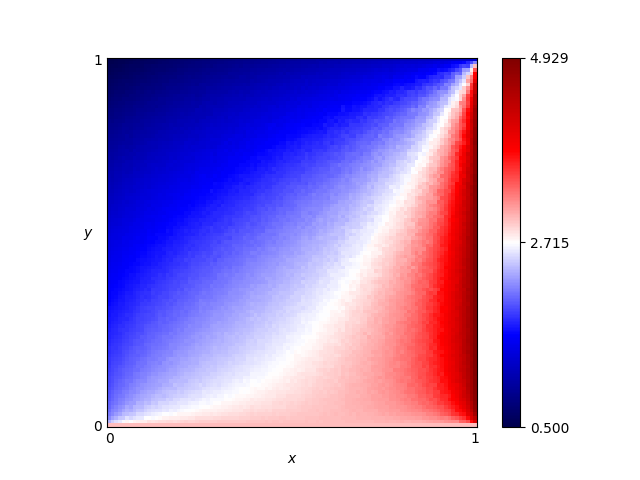
\includegraphics[height=.3\textheight]{src/chapters/chapters-02/Win-Stay_Lose-Shift.png}
    \caption{Pavlov fingerprinting with Tit for Tat used as the probe strategy.
    Figure was generated using~\cite{axelrodproject}.}
    \label{fig:fingerprinting}
\end{figure}

\begin{figure}[!hbtp]
    \centering
    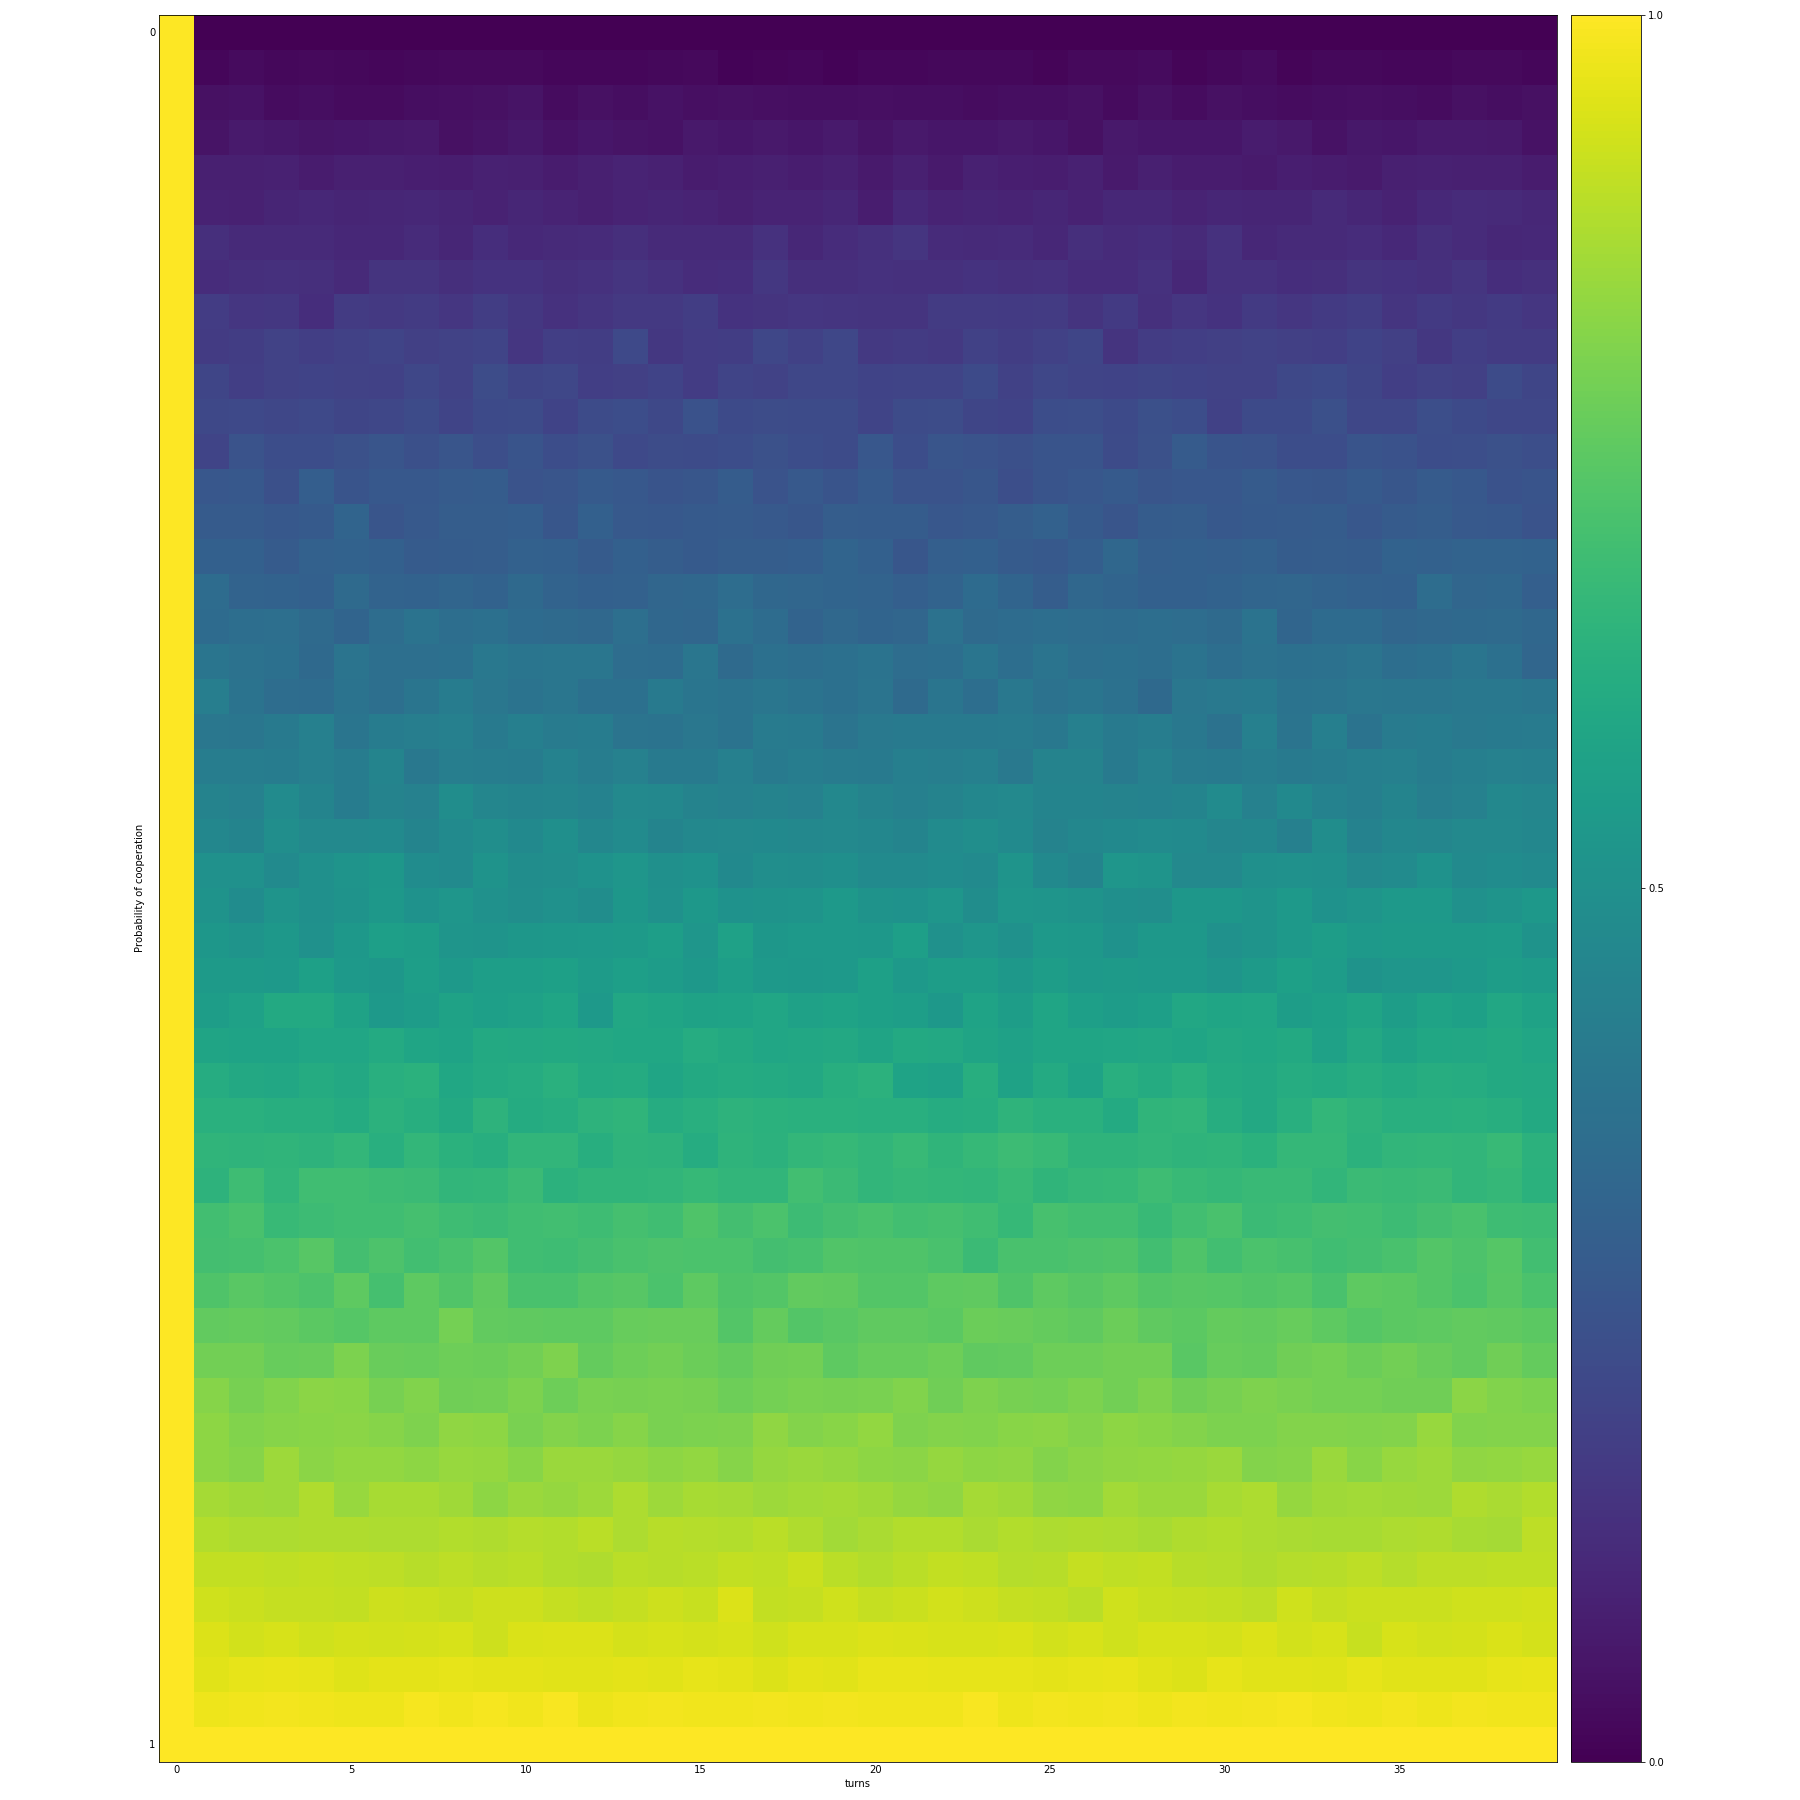
\includegraphics[height=.3\textheight]{src/chapters/chapters-02/Tit_for_Tat_fingerprint.png}
    \caption{Transitive fingerprint of Tit for Tat against a set of 50 random opponents.}
    \label{fig:transitive_fingerprinting}
\end{figure}

This section covered structured strategies and training methods. In the following
section software that has been developed with main aim simulating the IPD
is presented.

\section{Software}\label{section:software}

The research of the IPD heavily relies on software.
This is to be expected as computer tournaments have become the main
means of simulating the interactions in an IPD game.
Many academic fields suffer from lack of source code availability and the IPD
is not an exception. Several of the tournaments that have been discussed so far were generated
using computer code, though not all of the source code is available.
The code for Axelrod's original tournament is known to be lost and
moreover for the second tournament the only source code available is the code
for the 62 strategies (found on Axelrod's personal website~\cite{fortan_code}).

Several projects, however, are open, available and have been used as research
tools or educational platforms over the years. Two research tools~\cite{prison,
axelrodproject} and two educational tools~\cite{pd_trust, pd_game} are briefly
mentioned here. Both~\cite{prison, axelrodproject} are open
source projects.
The ``Game of Trust"~\cite{pd_trust} is an on-line, graphical user interface
educational platform for learning the basics of game theory, the IPD
and the notion of strategies. It attracted a lot of attention
due to being ``well-presented with scribble-y hand drawn
characters''~\cite{trust_blogb} and ``a whole heap of fun''~\cite{trust_bloga}.
Finally~\cite{pd_game} is a personal project written in PHP. It is a graphical user
interface that offers a big collection of strategies and allows the user to try
several matches and tournament configurations.

PRISON~\cite{prison} is written in the programming
language Java and a preliminary version was launched on 1998. It was used by its
authors in several publications, such as~\cite{Beaufils1997}, which introduced
Gradual, and~\cite{Beaufils1988}. The project includes a good number of
strategies from the literature but unfortunately the last update of the project
dates back to 2004. Axelrod-Python~\cite{axelrodproject} is a software used
by~\cite{Knight2017,KnightHGC17, Goodman2018, Wang2017}. It is written in the
programming language Python following best practice approaches~\cite{Aberdour2007,
Benureau2018} and contains the
largest collection of strategies, known to the author. The strategy list of
the project has been cited by publications~\cite{Anastassacos2018, Hayes2017,
Neumann2018}.

\section{Conclusion}

This manuscript presented a literature review on the Iterated Prisoner's
Dilemma. The opening sections focused on research trends and published works of
the field, followed by a presentation of research and educational software.
More specifically, Section~\ref{section:origin}
covered the early years of research. This was when simulating turns of the game
was only possible with human subject research.
Following the early years, the pioneering tournaments of Axelord were introduced in
Section~\ref{section:intelligent_design}. Axelrod's work offered the field an
agent based game theoretic framework to study the IPD.
In his original papers he asked researchers to design strategies to test their
performance with the new framework. The winning strategy of both his tournaments
was Tit for Tat. The strategy however came with limitations which were explored
by other researchers, and new intelligently designed strategies were introduced in
order to surpass Tit for Tat with some contributions such as Pavlov and Gradual.

Soon researchers came to realise that strategies should not just do well in a tournament setting
but should also be evolutionary robust. Evolutionary dynamic methods were
applied to many works in the field, and factors under which cooperation
emerges were explored, as described in Section~\ref{section:evolutionary_dynamics}.
This was not done only for unstructured populations, where all strategies
in the population can interact with each other, but also in population where
interactions were limited to only strategies that were close to each other.
In such topologies it was proven that even in the one shot game, cooperation can
indeed emerge.

Evolutionary approaches can offer many insights in the study of the PD. In
evolutionary settings strategies can learn to adapt and take over population by
adjusting their actions; such algorithms can be applied so that evolutionarily
robust strategies can emerge. Algorithms and structures used to train strategies
in the literature were covered in Section~\ref{section:structured_strategies}.
From these training methods several strategies are found,
and to be able to differentiate between them fingerprinting was
introduced. The research of best play and cooperation has been going on since
the 1950s, and for simulating the game software has been developed along the
way. This software has been briefly discussed
in Section~\ref{section:software}.

The study of the PD is still an ongoing field research where new variants and
new structures of strategies are
continuously being explored~\cite{Ohtsuki2018}. The game now serves as a model
in a wide range of applications, for example in medicine and the study of cancer
cells~\cite{archetti2018, Kaznatchee2017}, as well as in social situations and
how they can be driven by rewards~\cite{Dridi2018}. New research is still ongoing
for example in evolutionarily dynamics on graphs~\cite{Allen2017, hathcock2018,
Liu2017}.

% \newpage
% \bibliographystyle{plain}
% \bibliography{bibliography.bib}
\chapter{A bibliometric study of research topics, collaboration and influence in
the field of the Iterated Prisoner's Dilemma}

This manuscript explores the research topics and collaborative behaviour of
authors in the field of the Prisoner's Dilemma using topic modeling and a graph
theoretic analysis of the co-authorship network. The analysis identified five
research topics in the Prisoner's Dilemma which have been relevant of the course
of time. These are human subject research, biological studies, strategies,
evolutionary dynamics on networks and modeling problems as a Prisoner's Dilemma
game. Moreover, the results demonstrated the Prisoner's Dilemma is a field of
continued interest, and although it is a collaborative field, it is not
necessarily more collaborative than other scientific fields. The co-authorship
network suggests that authors are focused on their communities and not many
connections across the communities are made. The Prisoner Dilemma authors also
do not influence or gain much information by their connections, unless they are
connected to a ``main'' group of authors.

\section{Introduction}\label{section:introduction}

The Prisoner's Dilemma (PD) is a well known game used since its introduction in
the 1950's~\cite{Flood1958} as a framework for studying the emergence of
cooperation; a topic of continued interest for mathematical,
social~\cite{Perc2008}, biological~\cite{Turner1999} and
ecological~\cite{Wu2011} sciences. This manuscript presents a bibliometric
analysis of 2,420 published articles on the Prisoner's Dilemma between 1951 and
2018. It presents the dominant topics in the PD publications, which have been
identified using Latent Dirichlet Allocation~\cite{Blei2003}, and it explores the changes in the
dominant topics over time. The collaborative behaviour of the field is explored
using the co-authorship network, and furthermore, the Latent Dirichlet
Allocation topic analysis is combined with the co-authorship network analysis to assess
the relative influence of authors in these topics. Assessing the collaborative
behaviour of the field of collaboration itself is the main aim of this work.

As discussed in~\cite{youngblood2018}, bibliometrics (the statistical analysis
of published works originally described by~\cite{pritchard1969}) has been used
to support historical assumptions about the development of fields
\cite{raina1998}, identify connections between scientific growth and policy
changes \cite{das2016}, develop a quantitative understanding of author
order~\cite{sekara2018}, and investigate the collaborative structure of an
interdisciplinary field~\cite{Liu2015}. Most academic research is undertaken in
the form of collaborative effort and as~\cite{Kyvik2017} points out, it is
rational that two or more people have the potential to do better as a group
than individually. Indeed this is the very premise of the Prisoner's Dilemma itself.
Collaboration in groups has a long tradition in experimental
sciences and it has be proven to be productive according
to~\cite{Etzkowitz1992}. The number of collaborations can be different
between research fields and understanding how collaborative a field is not
always an easy task. Several studies tend to consider academic citations as a
measure for these things. A blog post published by Nature~\cite{nature_blog}
argues that depending on citations can often be misleading because the true
number of citations can not be known. Citations can be missed due to data entry
errors, academics are influenced by many more papers than they actually cite and
several of the citations are superficial.

A more recent approach to measuring collaborative behaviour, and to studying the
development of a field is to use the co-authorship network, as described
in~\cite{Liu2015}. The co-authorship network has many advantages as several
graph theoretic measures can be used as proxies to explain author relationships.
For example the average degree of a node corresponds to the average number of
an authors' collaborators, and clustering coefficient corresponds to the extent that
two collaborators of an author also collaborate with each other.
In~\cite{Liu2015}, the approach was applied to analyse the development of the field
``evolution of cooperation'', and in~\cite{youngblood2018} to identify the
subdisciplines of the interdisciplinary field of ``cultural evolution'' and
investigate trends in collaboration and productivity between these subdisciplines.
Moreover, \cite{Li2019} examined the
long-term impact of co-authorship with established, highly-cited scientists on
the careers of junior researchers. This paper builds upon the work done
by~\cite{Liu2015} and ~\cite{youngblood2018}, and extends their methodology.
In \cite{Liu2015, youngblood2018}, a data set from a
single source, Web of Science, is considered whereas the data set described here, archived
at~\cite{pd_data_2018}, has been collected from five sources.

Latent Dirichlet Allocation (LDA) is a topic modeling technique proposed
in~\cite{Blei2003} as a generative probabilistic model for discovering
underlying topics in collections of data.
Applications of the technique include detection in image data~\cite{Agarwal2008,
Coelho2010} and detection in video~\cite{Niebles2008, Wang2008}. Nevertheless,
LDA has been applied by several works on publication data for identifying the
topic structure of a subject area. In~\cite{Inglis2018}, it was applied to the
publications on mathematical education of the journals ``Educational Studies in
Mathematics'' and ``Journal for Research in Mathematics Education'' to
identify the dominant topics that each journal was publishing on. The topics of
the North American library and Information Science dissertations were 
studied chronologically in~\cite{Sugimoto2011}, and the main topic of the
scientific content presented at EvoLang conferences was identified
in~\cite{Bergmann2018}. In~\cite{Bergmann2018} the LDA approach is combined with
clustering and a co-authorship network analysis. A clustering analysis is
applied to the LDA topics, and the co-authorship network is analysed as a whole
where the clusters are only used to differentiate between the authors' topics.
In comparison, this works applies
LDA to identify dominant topics in the Prisoner's Dilemma fields and analyses
the networks corresponding to these topics individually.

The methodology used in this manuscript (including the data collection) is
covered in Section~\ref{section:methodology} and a preliminary analysis of the
data set is presented in Section~\ref{section:preliminary}. This manuscript
makes usage of the methodology and data to address the following questions:

\begin{enumerate}
    \item What are the research topics of the Prisoner's Dilemma?
    \item Is one topic currently more in fashion?
    \item How have the research topics changed over the years?
    \item Is the Prisoner's Dilemma a collaborative field?
    \item Are some topics more collaborative than others?
    \item Are there authors which benefit more from their position in the
    network?
\end{enumerate}

Results regarding questions 1-3 are presented in Section~\ref{section:topics}
and questions 4-6 are addressed in Section~\ref{section:co_authorship}. The
results are summarised in Section~\ref{section:conclusion}.

\section{Methodology}\label{section:methodology}

Academic articles are accessible through scholarly databases. Several databases
and collections today offer access through an open application protocol
interface (API). An API allows users to query directly a journal's database and
bypass the graphical user interface. Interacting with an API has two phases:
requesting and receiving. The request phase includes composing a url with the
details of the request. For example,
\url{http://export.arxiv.org/api/query?search_query=abs:prisoner's
dilemma&max_results=1} represents a request message. The first part of the
request is the address of the API. In this example the address corresponds to
the API of arXiv. The second part of the request contains the search arguments.
In this example it is requested that the word `prisoners dilemma' exists within
the article's title. The format of the request message is different from API to
API. The receive phase includes receiving a number of raw metadata of articles
that satisfies the request message. The raw metadata are commonly received in
extensive markup language (xml) or Javascript object notation (json)
formats~\cite{nurseitov2009}. Similarly to the request message, the structure of
the received data differs from journal
to journal.

The data collection is crucial to this study. To ensure that this study can be
reproduced all code used to query the different APIs has been packaged as a
Python library and is available online~\cite{nikoleta_2017}. The software could
be used for any type of projects similar to the one described here,
documentation for it is available at:
\url{http://arcas.readthedocs.io/en/latest/}. Project~\cite{nikoleta_2017} allow
users to collect articles from a list of APIs by specifying just a single
keyword. Articles for which any of the terms ``prisoner's dilemma'',
``prisoners dilemma'', ``prisoner dilemma'', ``prisoners evolution'', ``prisoner
game theory'' existed within the title, the abstract or the text are included
in the analysis. Four prominent journals in the field and a preprint server
were used as sources to collect data for this analysis:

\begin{multicols}{2}
    \begin{itemize}
        \item arXiv~\cite{mckiernan2000}; a repository of electronic preprints.
        It consists of scientific
        papers in the fields of mathematics, physics, astronomy, electrical engineering,
        computer science, quantitative biology, statistics, and quantitative finance,
        which all can be accessed online.
        \item PLOS~\cite{plos}; a library of open access journals and other scientific literature
        under an open content license. It launched its first journal, PLOS Biology,
        in October 2003 and publishes seven journals, as of October 2015.
        \item IEEE Xplore Digital Library (IEEE)~\cite{ieee}; a research database for discovery
        and access to journal articles, conference proceedings, technical standards,
        and related materials on computer science, electrical engineering and electronics,
        and allied fields. It contains material published mainly by the Institute of
        Electrical and Electronics Engineers and other partner publishers. 
        \item Nature~\cite{nature}; a multidisciplinary scientific journal,
        first published on 4 November 1869. It was ranked the world's most cited
        scientific journal by the Science Edition of the 2010 Journal Citation Reports
        and is ascribed an impact factor of 40.137, making it one of the world's
        top academic journals.
        \item Springer~\cite{springer}; a leading global scientific publisher of
        books and journals. It publishes close to 500 academic and professional
        society journals.
    \end{itemize}
\end{multicols}

The data set has been archived and is available at~\cite{pd_data_2018}. Note that the latest data
collection was performed on the \(30^{\text{th}}\) November 2018.
% TODO Ensure this stay accurate

The relationship between the authors within a field will be modeled as a graph
\(G = (V_G, E_G)\) where \(V_G\) is the set of nodes and \(E_G\)  is the set of
edges. The set \(V_G\) represents the authors and an edge connects two authors
if and only if those authors have written together. This co-authorship network is
constructed using the main data set~\cite{pd_data_2018} and the open source package
\cite{networkx}. The PD network is denoted as \(G\) where the
number of unique authors \(|V(G)|\) is \authors and \(|E(G)|\) is \edges.
All authors' names were formatted as their first name and last name (i.e.
Martin A. Nowak to Martin Nowak). This was done to avoid errors such as Martin
A. Nowak and Martin Nowak being treated as a different person. There are some
authors for which only their first initial was found. These entries are left as
such.

The collaborativeness of the authors will be analysed using measures such as, isolated nodes,
connected components, clustering coefficient, communities, modularity and average degree.
These measures show the number of connections authors can have
and how strongly connected these people are. The number of isolated nodes is the
number of nodes that are not connected to another node, thus the
number of authors that have published alone. The average degree denotes the average
number of neighbours for each nodes, i.e. the average number of collaborations
between the authors.
A connected component is a maximal set of nodes such that each pair of nodes is
connected by a path~\cite{Easley2010}. The number of connected components as well as the size of the
largest connected component in the network are reported.
The size of the largest connected component represents the scale of the central cluster
of the entire network, as will be discussed in the analysis section.
Clustering coefficient and modularity are also calculated. The clustering
coefficient, defined as 3 times the number of triangles on the graph divided
by the number of connected triples of nodes, is a local measure of the degree to
which nodes in a graph tend to cluster together
in a clique~\cite{Easley2010}. It shows to which extent the collaborators
of an author also write together.
In comparison, modularity is a global measure designed to measure the strength of
division of a network into communities. The number of communities will be reported
using the Clauset-Newman-Moore method~\cite{clauset2004}. Also the modularity index
is calculated using the Louvain method described in~\cite{Blondel2008}. The value
of the modularity index can vary between \([-1, 1]\), a high value of modularity
corresponds to a structure where there are dense connections between the nodes within
communities but sparse connections between nodes in different communities.
That means that there are many sub communities of authors that write together
but not across communities.
Two further points are aimed to be explored in this work, (1) which people control the flow
of information;
as in which people influence the field the most and (2) which are the authors that
gain the most from the influence of the field. To measure these concepts
centrality measures are going to be used.
Centrality measures are often used to understand different
aspects of social networks~\cite{Landherr2010}. Two centrality measures have been
chosen for this paper and these are closeness and betweenness centrality.

\begin{enumerate}
    \item In networks some nodes have a short distance to a lot of nodes and
    consequently are able to spread information on the network very effectively.
    A representative of this idea is \textbf{closeness centrality}, where a node
    is seen as centrally involved in the network if it requires only few
    intermediaries to contact others and thus is structurally relatively
    independent. Closeness centrality is interpreted as influence. Authors with a high
    value of closeness centrality, are the authors that spread scientific
    knowledge easier on the network and they have high influence.
    \item Another centrality measure is the \textbf{betweenness centrality},
    where the determination of an author's centrality is based on the quotient
    of the number of all shortest paths between nodes in the network that
    include the node in question and the number of all shortest paths in the
    network. In betweenness centrality the position of the node matters. Nodes
    with a higher value of betweenness centrality are located in positions that
    a lot of information pass through, this is interpreted as the gain from
    the influence, thus these authors gain the most from their networks.
\end{enumerate}

The articles contained in the data set (\cite{pd_data_2018}) will be classified
into research topics using LDA an unsupervised machine learning technique
designed to summarize large collections of documents by a small number of
conceptually connected topics or themes~\cite{Blei2003, Grimmer2013}. The
documents are the articles' abstracts and LDA was carried out using~\cite{rehurek_lrec}.
In LDA, each document/abstract is represented by a distribution over topics,
and the topics themselves are represented by a distribution over words. More
specifically, each topics is described by weights associated with words and
each document by the probabilities of belonging to a specific topic. The
probability of a document belonging to a topic is referred to as the percentage
contribution denoted as \(c\). For example the words and their associated
weights for two topics A and B could be:

\begin{itemize}
    \item Topic A: \(0.039 \times\)``cooperation'', \(0.028 \times\)``study'' and \(0.026 \times\)``human''.
    \item Topic B: \(0.020 \times\)``cooperation'', \(0.028 \times\)``agents'' and
    \(0.026 \times\)``strategies''.
\end{itemize}

The percentage contribution for a document with abstract ``The study of
cooperation in humans'' has a \(c_{A} = 0.039 + 0.028 + 0.026 = 0.093\) and
\(c_B = .020 + 0.0 + 0.0 = 0.020\). The topic to which a document is assigned to
is based on the highest percentage contribution denoted as \(c^*\). For the
given example the dominant topic is Topic A \(c^*=c_A\). LAD requires that
the number of topics is specified in advance before running the algorithm. The
number of topics can be chosen using the coherence value~\cite{Roder2015} or
through subjective minimisation of the overlapping keywords between two topics.
Both these approaches will be used in this work.

Several of the approaches described in this section have previously been
carried out in~\cite{Bergmann2018,Liu2015,Sugimoto2011, youngblood2018},
the novelty here is combining the approaches as well as applying them
to a new data set. A preliminary analysis of the data set is presented in the
following section.

\section{Preliminary Analysis}\label{section:preliminary}

The data set~\cite{pd_data_2018} consists of \totalarticles articles with unique
titles. In case of duplicates the preprint version of an article (collected from
arXiv) was dropped. Similarly to~\cite{Liu2015}, \manual articles have not been
collected from the aforementioned APIs but have been manually added because they
are of interest. Examples of such papers include~\cite{Flood1958}
the first publication on the PD,~\cite{Ohtsuki2006, Stewart2012} two well cited
articles in the field, and a series of works from Robert Axelrod
~\cite{Axelrod1980, Axelrod1980more, Axelrod1987, Axelrod1981, Riolo2001} a
leading author of the field. A more detailed summary of the articles' provenance
is given by Table~\ref{table:preliminary_table}. Only 3\% of the data set consists of
articles that were manually added and 27\% of the articles were collected from
arXiv. The average number of publications is also included in
Table~\ref{table:preliminary_table}. Overall an average of 43 articles are published
per year on the topic. The most significant contribution to this appears to be
from arXiv with 11 articles per year, followed by Springer with 9 and PLOS with
8.

\begin{table}[!hbtp]
    \begin{center}
    \resizebox{.9\textwidth}{!}{
    \begin{tabular}{lrrrr}
\toprule
{} &  Number of Articles &  Percentage \% &  Year of first publication &  Average number of publications per year\\
\midrule
IEEE     &               294 &       12.14\% &                    1973 &                             5\\
Manual   &                76 &        3.14\% &                    1951 &                             1\\
Nature   &               436 &       18.00\% &                    1959 &                             8\\
PLOS     &               477 &       19.69\% &                    2005 &                             8\\
Springer &               533 &       22.01\% &                    1966 &                             9\\
arXiv    &               654 &       27.00\% &                    1993 &                            11\\
Overall  &              2470 &      100.00\% &                    1951 &                            43\\
\bottomrule
\end{tabular}
}
    \end{center}
    \caption{Summary of~\cite{pd_data_2018} per provenance.}
    \label{table:preliminary_table}
\end{table}

The data handled  here is in fact a time series from the 1950s, the formulation
of the game, until 2018 (Figure~\ref{fig:timeseries}). Two observations can be
made from Figure~\ref{fig:timeseries}.

\begin{enumerate}
    \item There is a steady increase of the number of publications since the
    1980s and the introduction of computer tournaments~\cite{Axelrod1981}
    (work by Robert Axelrod).
    \item There is a decrease in 2017-2018. This is due to our data set being
    incomplete. Articles that have been written in 2017-2018 have either not
    being published or were not retrievable by the APIs at the time of the last
    data collection.
\end{enumerate}

These observations can be confirmed by studying the time series.
Using~\cite{scipy}, an exponential distribution is fitted to the data.
The fitted model can be used to forecast the
behaviour of the field for the next 5 years. Even
though the time series has indicated a slight decrease, the model forecasts that
the number of publications will keep increasing, thus demonstrating that the
field of the PD continues to attract academic attention.

\begin{figure}[!hbtp]
    \centering
    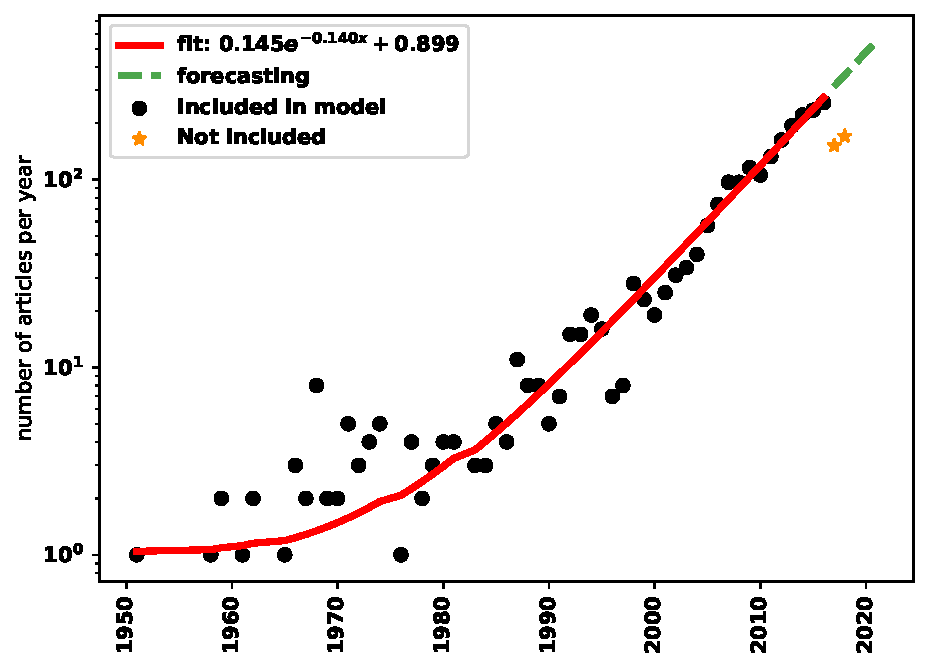
\includegraphics[width=.50\textwidth]{src/chapters/chapters-03/paper/Literature-Article/assets/images/forecasting.pdf}
    \caption{Number of articles published on the PD 1951-2018 (on a log scale),
    with a fitted exponential line, and a forecast for 2017-2022.}\label{fig:timeseries}
\end{figure}

There are a total of \authors authors in the data set (\cite{pd_data_2018}) and several of these
authors have had multiple publications collected from the data collection process.
The highest number of articles collected for an
author is 83 publications for Matjaz Perc. The distribution of the number of
papers per author is given by Figure~\ref{fig:num_papers_per_author}, and it can
be seen that Matjaz Perc is an outlier. More specifically, most authors have
1 to 6 publications in the data set.

\begin{figure}[!hbtp]
    \centering
    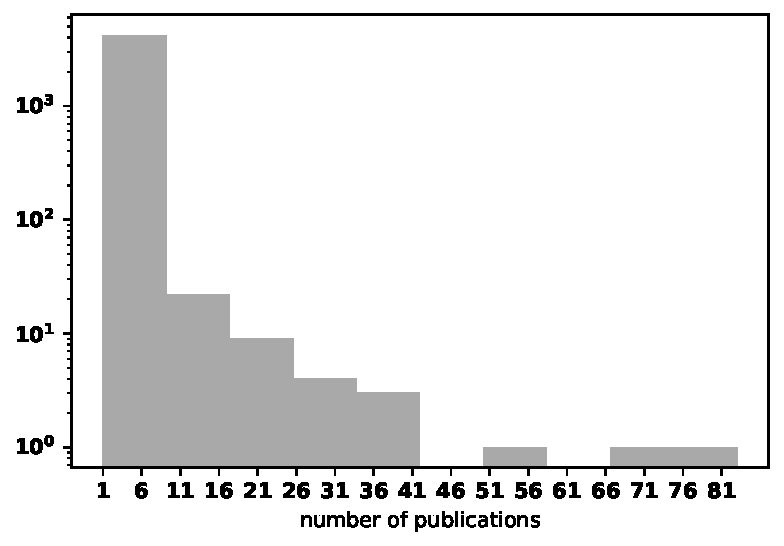
\includegraphics[width=.50\textwidth]{src/chapters/chapters-03/paper/Literature-Article/assets/images/papers_per_author.pdf}
    \caption{Distribution of number of papers per author (on a log scale).}
    \label{fig:num_papers_per_author}
\end{figure}

The overall Collaboration Index (CI) or the average number of authors on
multi-authored papers is 3.2, thus on average a non single author publication in
the PD has 3 authors. This appears to be quite standard compared to other fields
such as cultural evolution~\cite{youngblood2018}, Astronomy and Astrophysics,
Genetics and Heredity, Nuclear and Particle Physics as reported
by~\cite{nature_author_blog}.
There are only a total of 545 publications with a single author, which
corresponds to the 22\% of the papers. It appears that academic publications
tend to be undertaken in the form of collaborative effort, which is in line
with the claim of~\cite{Kyvik2017}. From
Figure~\ref{fig:ci_over_time} the trend of CI over the years is given. There are
some peaks in the early years 1969 and 1980, however, a steady increase appears
to happen after 2004. This could be an effect of better communication tools
being introduced around that time which enabled more collaborations between
researchers.

\begin{figure}[!hbtp]
    \centering
    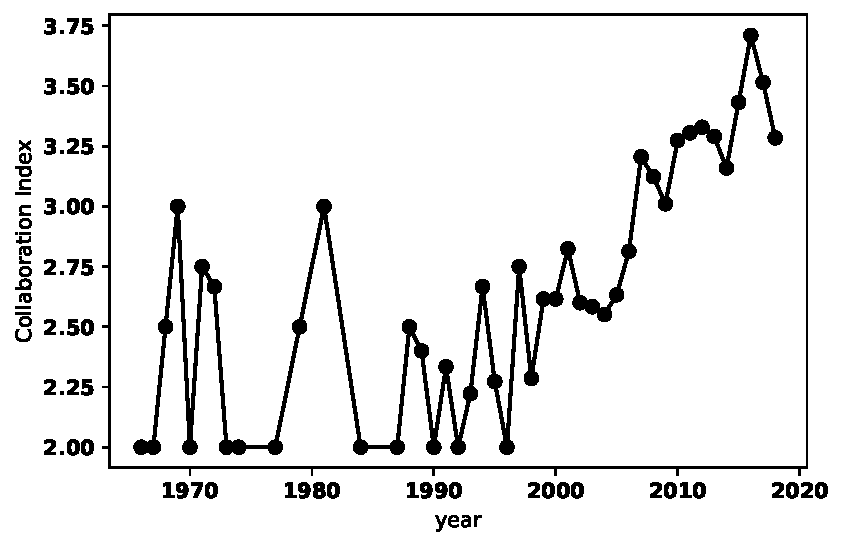
\includegraphics[width=.55\textwidth]{src/chapters/chapters-03/paper/Literature-Article/assets/images/collaborative_index.pdf}
    \caption{Collaboration index over time.}\label{fig:ci_over_time}
\end{figure}

The collaborativeness of the authors is explored in more detail in
Section~\ref{section:co_authorship} using the co-authorship network. The
collaborative behaviour and relative influence of authors will also be explored
in co-authorship networks which correspond to their publications research topics.
These topics are presented in the next section.

\section{Research topics in the Prisoner's Dilemma research}\label{section:topics}

In order to identify the topics which are being discussed in the field of the
PD, the LDA algorithm implemented in~\cite{rehurek_lrec} is applied to the
abstracts of the data set. As mentioned before, the number of topics, which
will be denoted as \(n\), needs to be specified before running the algorithm.
The appropriate number of topics is chosen based on the coherence
value~\cite{Roder2015}. Figure~\ref{fig:coherence_value_over_number_of_topcis}
gives the coherence values of 18 models where \(n \in \{2, 3, \dots, 19\}\), and
it can be seen than the most appropriate number of topics is 6 with a coherence
value of 0.418.

\begin{figure}[!hbtp]
    \centering
    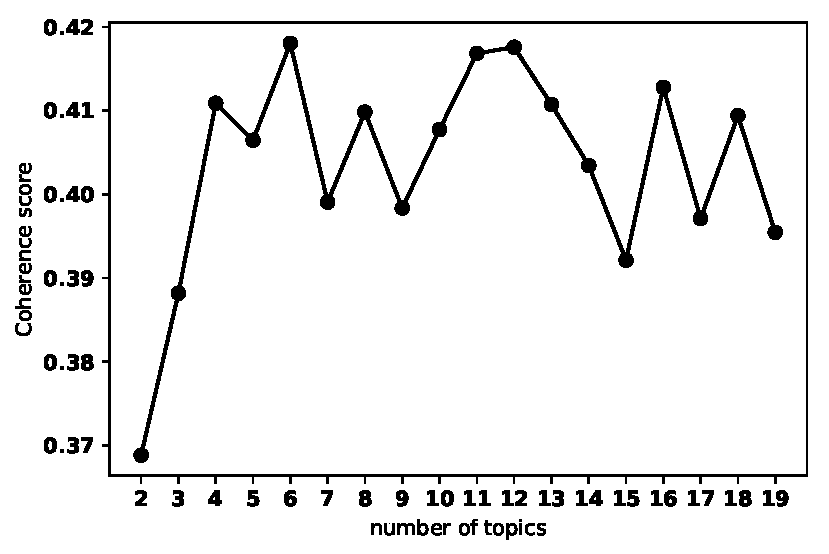
\includegraphics[width=.45\textwidth]{src/chapters/chapters-03/paper/Literature-Article/assets/images/coherence_values.pdf}
    \caption{Coherence for LDA models over the number of topics.}
    \label{fig:coherence_value_over_number_of_topcis}
\end{figure}

An LDA model outputs an \(N \times n\) matrix - \(N\) rows for \(N\)
abstracts and \(n\) columns for \(n\) topics. The cells contain the percentage
contributions for each topic for each abstract, \(c_i^ j\) for
\(i \in \{1, 2, \dots, n\}\) for \(j \in \{1, 2, \dots, N\}\). In essence,
LDA maps every paper to a vector space of dimension the number of topics. In the case
of 6 topics it is difficult to visualise the clustering of topics. To overcome
this a dimensionality reduction approach called t-Distributed Stochastic Neighbor Embedding
(t-SNE)~\cite{Maaten2008} is applied to the LDA model outputs. More specifically,
t-SNE is used to reduce the dimensions of each \(c^j\) from \(n\) to 2.
Figure~\ref{fig:lda_visualisation_six}, gives the visualisation of LDA for \(n=6\).
Each point represents a single document and its color corresponds to the topic
with the highest percentage contribution. The documents which are clustered
together have a similar percentage contribution distribution over the topics.

Even though the LDA model with \(n=6\) has the highest coherence value, Figure
\ref{fig:lda_visualisation_six} shows that documents of the same topic are
closer to documents from other topics than each other. For example the documents
of topic 2 are divided into two clusters. The one cluster is closer to documents
from topic 4 and the other has a few documents closer to topic 1. In the case of \(n=6\)
topic 4 appears to be on ``evolution of cooperation on networks'', and the
papers from topic 2 surrounded from topic 4 include the articles
``Evolutionary prisoner's dilemma game on hierarchical lattices''~\cite{Vukov2005}
and ``Social evolution in structured populations''~\cite{Debarre2014}. Publications
that clearly also fit topic 4.

In comparison,
\ref{fig:lda_visualisation_five} gives the visualisation of LDA \(n=5\) where
the separation of the documents is more clear. Though
several models, Figure~\ref{fig:coherence_value_over_number_of_topcis}, have a
higher coherence value than the LDA model with \(n=5\), the separation
of topics is not as clear for any model as it is for \(n=5\). Thus, \(n=5\) is
chosen to carry out the analysis of this work, and moreover the LDA model for
\(n=5\) has a coherence value 0.406 which is close to 0.418.

\begin{figure}[!hbtp]
    \centering
    \begin{minipage}{.45\textwidth}
        \centering
        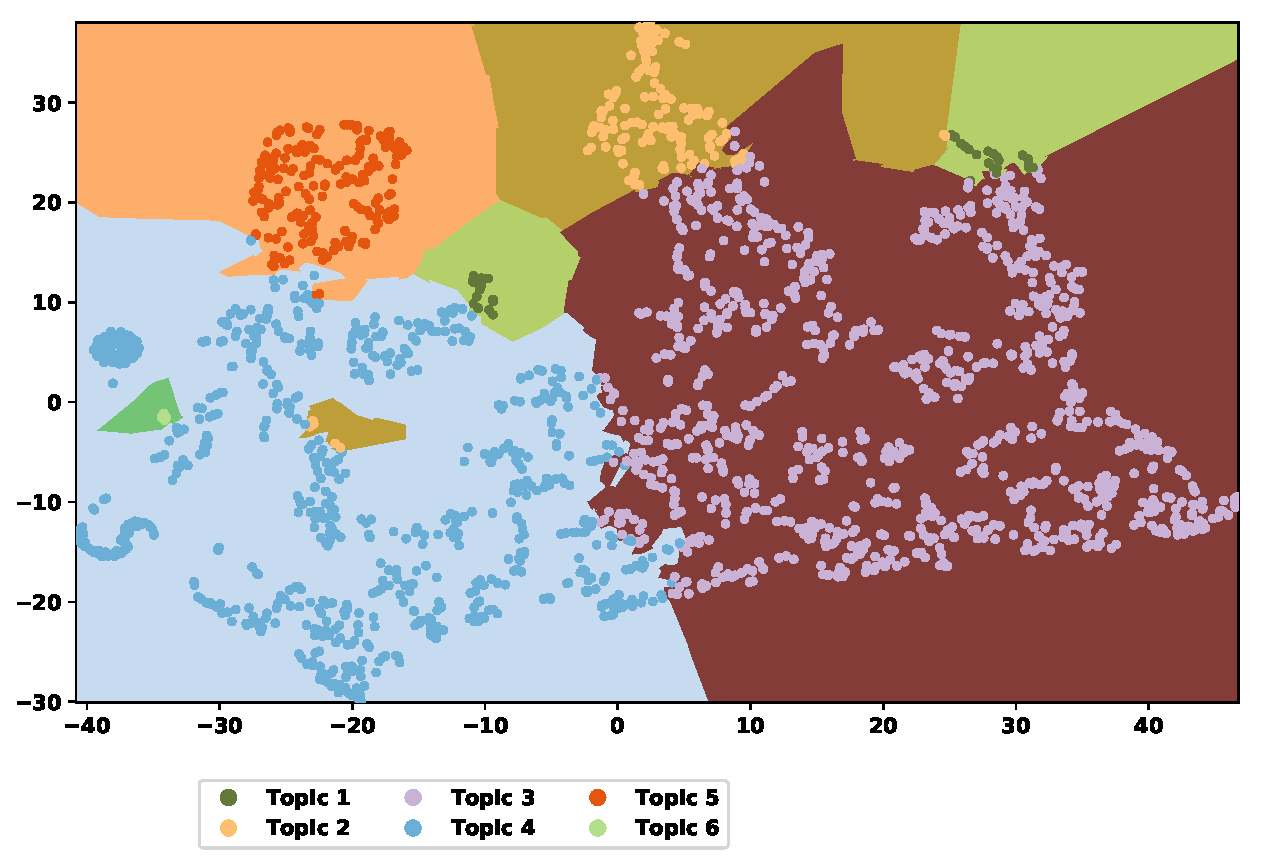
\includegraphics[width=.9\textwidth]{src/chapters/chapters-03/paper/Literature-Article/assets/images/topics_scatter_plot_6.pdf}
        \caption{Visualisation of LDA with \(n=6\) on 2 dimensions.}\label{fig:lda_visualisation_six}
    \end{minipage}\hfill
    \begin{minipage}{.45\textwidth}
        \centering
        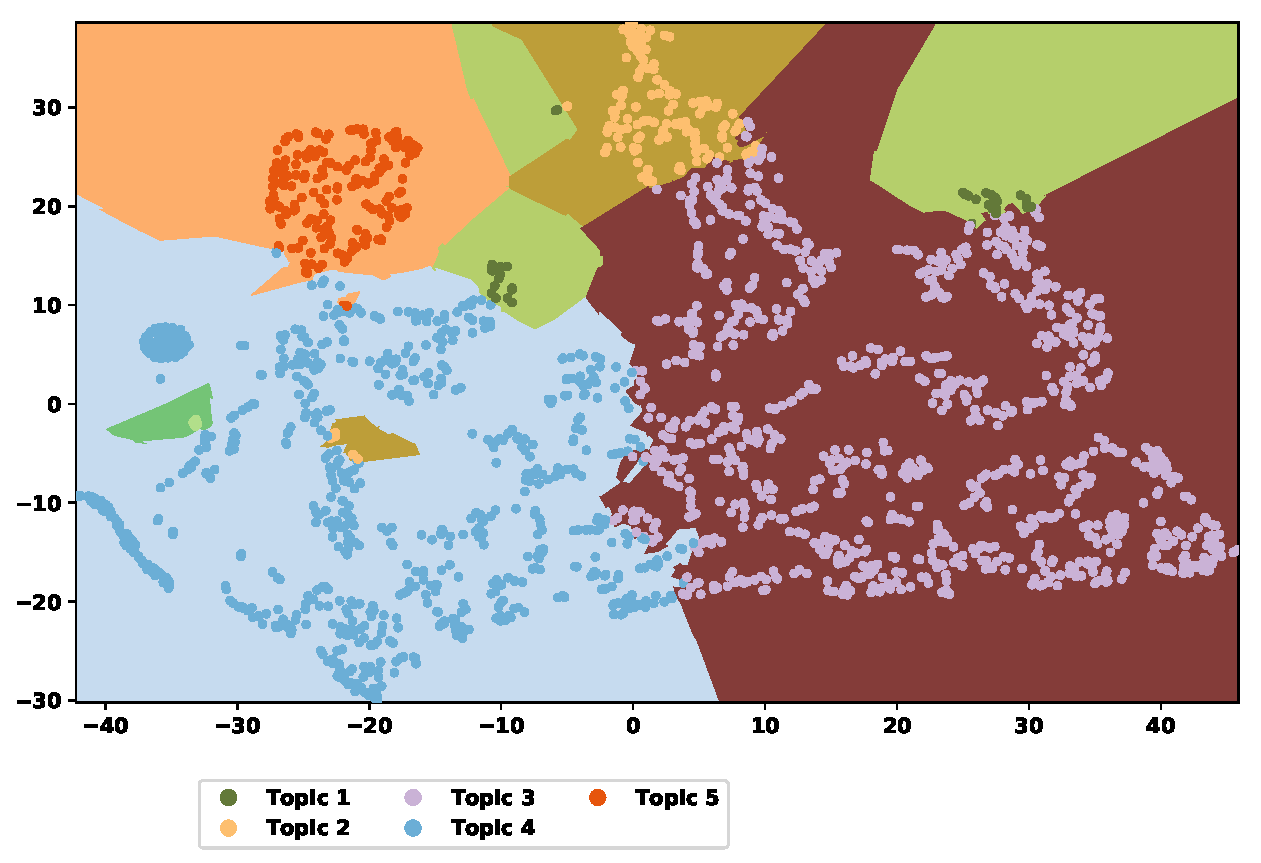
\includegraphics[width=.9\textwidth]{src/chapters/chapters-03/paper/Literature-Article/assets/images/topics_scatter_plot_5.pdf}
        \caption{Visualisation of LDA with \(n=5\) on 2 dimensions.}\label{fig:lda_visualisation_five}
    \end{minipage}
\end{figure}

\textbf{What are the research topics of the Prisoner's Dilemma?}

For \(n=5\) the articles are clustered and assigned to their dominant topic,
based on the highest percentage contribution. The keywords associated with a
topic, the most representative article of the topic (based on the
percentage contribution) and its academic reference are given by
Table~\ref{table:topics_and_articles}. The topics are labelled as A, B, C, D and
E, and more specifically:

\begin{itemize}
    \item Based on the keywords associated with Topic A, and the most
    representative article, Topic A appears to be about \textbf{human subject
    research}. Several publications assigned to the topic study the PD by
    setting experiments and having human participants simulate the game
    instead of computer simulations. These articles include~\cite{Matsumoto2016}
    which showed that prosocial behavior increased with the age of the
    participants, ~\cite{Li2014} which studied the difference in cooperation
    between high-functioning autistic and typically developing
    children,~\cite{Molina2013} explored the gender effect in highschool
    students and~\cite{Bell2017} explored the effect of facial expressions of
    individuals.
    \item Though it is not immediate from the keywords associated with
    Topic B, investigating the papers assigned to the topic indicate that it
    is focused on \textbf{biological studies}. Papers assigned to the topic include
    papers which apply the PD to genetics~\cite{Santorelli2008, Sistrom2015}, to
    the study of tumours~\cite{archetti2013evolutionary, sartakhti2017} and
    viruses~\cite{turner1999prisoner}. Other works include how phenotype affinity
    can affect the emergence of cooperation~\cite{wu2019phenotype} and modeling
    bacterial communities as a spatial structured social dilemma.
    \item Based on the keywords and the most representative article Topic
    C appears to include publications on PD \textbf{strategies}. Publications
    in the topic include the introduction of new strategies~\cite{stewart2013extortion},
    the search of optimality in strategies~\cite{banerjee2007reaching} and the
    training of strategies~\cite{ishibuchi2011evolution} with different
    representation methods. Moreover, publications that study the evolutionary
    stability of strategies~\cite{adami2013evolutionary} and introduced methods
    of differentiating between them~\cite{ashlock2008fingerprinting} are
    also assigned to C.
    \item The keywords associated with Topic D clearly show that the topic
    is focused on \textbf{evolutionary dynamics on networks}. Publications include
    \cite{ichinose2013robustness} which explored the robustness of cooperation
    on networks,~\cite{wang2012spatial} which studied the effect of a strategy's neighbourhood
    on the emergence of cooperation and~\cite{chen2016fixation} which explored
    the fixation probabilities of any two strategies is spatial
    structures.
    \item The publication assigned to Topic E are on \textbf{modeling problems
    as a PD game}. Though Topic B is also concerned with problems being formulated
    as a PD, it includes only biological problems. In comparison, the problems
    in Topic E include decision making in
    operational research~\cite{ormerod2010or}, information sharing among members
    in a virtual team~\cite{feng2008trilateral}, the measurement of influence
    in articles based on citations~\cite{hutchins2016relative} and the price
    spikes in electric power markets~\cite{Guan2002}, and not on biological studies.
\end{itemize}

\begin{table}[!hbtp]
    \begin{center}
    \resizebox{\textwidth}{!}{
    \begin{tabularx}{1.5\textwidth}{lXXl|cc}
\toprule
Dominant Topic &                                                                                                 Topic Keywords &                                                                                                                                    Most Representative Article Title &        Reference &  \# Documents &  \% Documents \\
\midrule
A &                 social, behavior, human, study, experiment, cooperative, cooperation, suggest, find, behaviour &                                                                                      Facing Aggression: Cues Differ for Female versus Male Faces &  \cite{Geniole2012} &                496.0 &                   0.2008 \\
B &                               individual, group, good, show, high, increase, punishment, cost, result, benefit &  Genomic and Gene-Expression Comparisons among Phage-Resistant Type-IV Pilus Mutants of Pseudomonas syringae pathovar phaseolicola &  \cite{Sistrom2015} &                309.0 &                   0.1251 \\
C &                             game, strategy, player, agent, dilemma, play, payoff, state, prisoner, equilibrium &                                                            Fingerprinting: Visualization and Automatic Analysis of Prisoner's Dilemma Strategies &  \cite{Sistrom2015} &                561.0 &                   0.2271 \\
D &  cooperation, network, population, evolutionary, evolution, interaction, dynamic, structure, cooperator, study &                                                   Influence of initial distributions on robust cooperation in evolutionary  Prisoner's Dilemma &     \cite{Chen2007} &                556.0 &                   0.2251 \\
E &                           model, theory, base, system, problem, paper, propose, information, provide, approach &                                                                          Gaming and price spikes in electric power markets and possible remedies &     \cite{Guan2002} &                548.0 &                   0.2219 \\
\bottomrule
\end{tabularx}
}
    \end{center}
    \caption{Keywords for each topic and the document with the most representative article for each topic.}
    \label{table:topics_and_articles}
\end{table}

Note that the whilst for the choice of 5 topics the actual clustering is not
subjective (the algorithm is determining the output) the interpretation above is.

\textbf{Five topics in the PD publications identified by the data set of this
work are human subject research, biological studies, strategies, evolutionary
dynamics on networks and modeling problems as a PD}.

These 5 topics nicely
summarise the PD research. They highlight the interdisciplinarity of the field;
how it brings together applied modeling of real world situations (Topic B and E)
and more theoretical notions such as evolutionary dynamics and optimality of
strategies.

\textbf{Is one topic currently more in fashion?}

Figure~\ref{fig:number_of_articles_per_topic} gives the number of articles
per topic over time. The topics appear to have had a similar trend over the years,
with topics B and D having a later start. Following the introduction of a topic
the publications in that topic have been increasing. There is no decreasing
trend in any of the topics. All the topics have been publishing for years and
they still attract the interest of academics. Thus, \textbf{there does not
seem to be any given topic more or less in fashion}.

\begin{figure}[!hbtp]
    \centering
    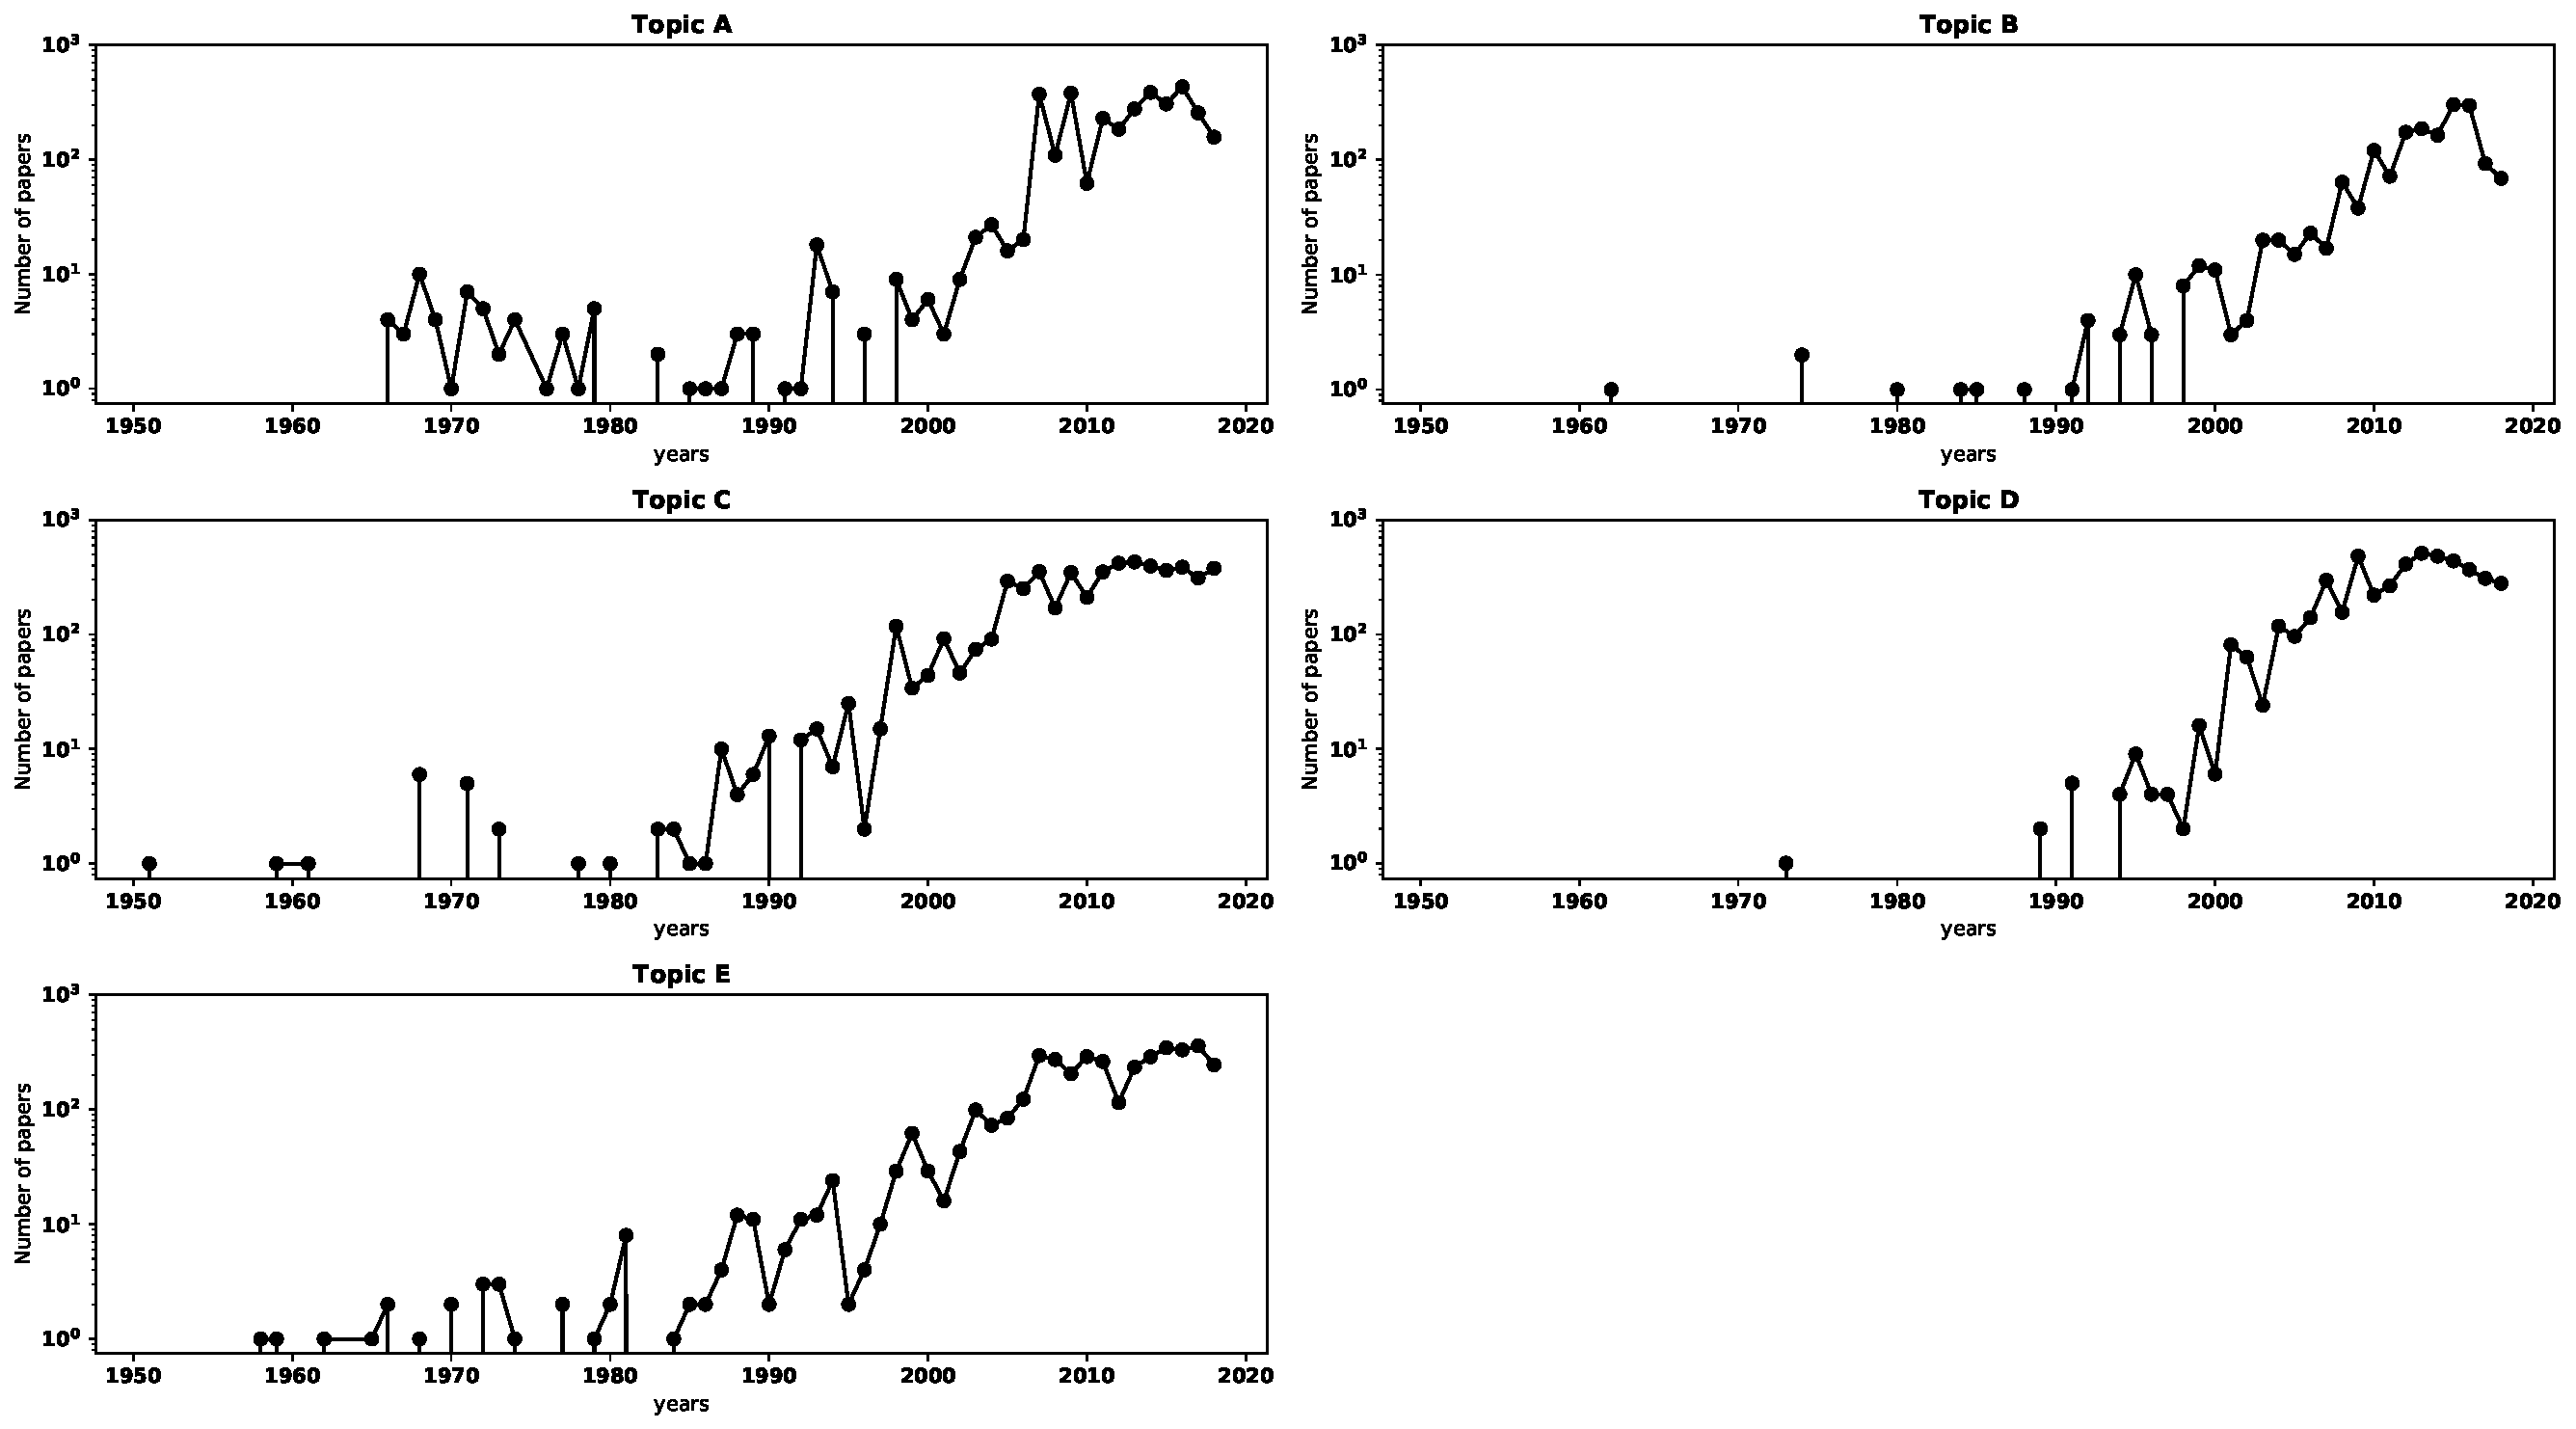
\includegraphics[width=\textwidth]{src/chapters/chapters-03/paper/Literature-Article/assets/images/papers_per_topic_over_time.pdf}
    \caption{Number of articles per topic over the years (on a logged scale).}\label{fig:number_of_articles_per_topic}
\end{figure}

\textbf{How do the research topics change over the years?}

To gain a better understanding regarding the change in the topics over the years,
LDA is applied to the cumulative data set over 8 time periods. These periods are
1951-1965, 1951-1973, 1951-1980, 1951-1988, 1951-1995, 1951-2003, 1951-2010,
1951-2018. The number of topics for each cumulative subset is chosen based on
the coherence value and no objective approach is used. As a result, the period
1951-2018 has been assigned \(n=6\) which had the highest coherence
value instead of 5. The chosen models for each period including the
number of topics, their keywords and number of articles assigned to them are
given by Table \ref{table:topics_per_year}.

\begin{table}[!hbtp]
    \begin{center}
    \resizebox{\textwidth}{!}{
    \begin{tabular}{llccc}
\toprule
    Period &  Topic &                                                                                                Topic Keywords & Num of Documents & Percentage of Documents \\
\midrule
 1951-1965 &               1 &                 problem, technology, divert, euler, subsystem, requirement, trace, technique, system, untried &                3 &                   0.375 \\
 1951-1965 &               2 &            interpret, requirement, programme, evolution, article, increase, policy, system, trace, technology &                2 &                    0.25 \\
 1951-1965 &               3 &          equipment, agency, conjecture, development, untried, programme, trend, technology, weapon, technique &                1 &                   0.125 \\
 1951-1965 &               4 &                 variation, celebrated, trend, untried, change, involve, month, technique, subsystem, research &                1 &                   0.125 \\
 1951-1965 &               5 &                           give, good, modern, trace, technique, ambiguity, problem, trend, technology, system &                1 &                   0.125 \\
 \midrule
 1951-1973 &               1 &                           study, shock, cooperative, money, part, vary, investigate, good, receive, equipment &               12 &                  0.3243 \\
 1951-1973 &               2 &          cooperation, level, significantly, sequence, reward, provoke, descriptive, principal, display, argue &                4 &                  0.1081 \\
 1951-1973 &               3 &               player, make, effect, triad, experimental, motivation, dominate, hypothesis, instruction, trend &                3 &                  0.0811 \\
 1951-1973 &               4 &                                           ss, sex, male, female, dyad, design, suggest, college, factor, tend &                3 &                  0.0811 \\
 1951-1973 &               5 &               result, research, format, change, operational, analysis, relate, understanding, decision, money &                2 &                  0.0541 \\
 1951-1973 &               6 &                          condition, give, high, treatment, conflict, cc, real, original, replication, promote &                2 &                  0.0541 \\
 1951-1973 &               7 &              group, competitive, show, interpret, scale, compete, escalation, free, variable, individualistic &                2 &                  0.0541 \\
 1951-1973 &               8 &                        outcome, strategy, choice, type, pdg, difference, dummy, conclude, compare, consistent &                2 &                  0.0541 \\
 1951-1973 &               9 &                   game, difference, pair, approach, behavior, person, weapon, occur, advantaged, differential &                2 &                  0.0541 \\
 1951-1973 &              10 &                    response, present, dilemma, influence, cooperate, bias, point, amount, participate, factor &                2 &                  0.0541 \\
 1951-1973 &              11 &                       trial, problem, previous, involve, prisoner, experiment, follow, tit, increase, initial &                1 &                   0.027 \\
 1951-1973 &              12 &                           matrix, behavior, rational, black, model, research, broad, distance, complex, trace &                1 &                   0.027 \\
 1951-1973 &              13 &                    play, finding, individual, noncooperative, white, nature, race, ratio, represent, prisoner &                1 &                   0.027 \\
 \midrule
 1951-1980 &               1 &                                      play, trial, group, follow, white, interpret, scale, black, trend, small &               14 &                    0.25 \\
 1951-1980 &               2 &                              outcome, level, effect, type, dyad, vary, pdg, participate, understanding, arise &                9 &                  0.1607 \\
 1951-1980 &               3 &         game, strategy, cooperation, significant, difference, sentence, text, occur, differential, hypothesis &                4 &                  0.0714 \\
 1951-1980 &               4 &                        male, female, find, result, sex, subject, experimental, situation, treatment, computer &                4 &                  0.0714 \\
 1951-1980 &               5 &                         research, problem, influence, matrix, format, model, analysis, year, crime, equipment &                4 &                  0.0714 \\
 1951-1980 &               6 &                                    condition, dilemma, bias, free, attempt, book, year, dummy, prison, design &                4 &                  0.0714 \\
 1951-1980 &               7 &                    variable, result, factor, individual, ability, triad, half, migration, change, investigate &                3 &                  0.0536 \\
 1951-1980 &               8 &                 show, present, suggest, rational, compete, approach, characteristic, examine, person, conduct &                3 &                  0.0536 \\
 1951-1980 &               9 &                         behavior, high, finding, relate, obtain, assistance, ratio, good, weapon, competition &                3 &                  0.0536 \\
 1951-1980 &              10 &                               ss, shock, money, competitive, part, difference, pair, amount, man, information &                3 &                  0.0536 \\
 1951-1980 &              11 &             player, conflict, theory, decision, determine, produce, maker, cooperate, specialist, programming &                2 &                  0.0357 \\
 1951-1980 &              12 &            study, prisoner, make, response, experiment, noncooperative, standard, separate, conclude, initial &                2 &                  0.0357 \\
 1951-1980 &              13 &                       give, cooperative, choice, cognitive, real, operational, set, subject, ascribe, concern &                1 &                  0.0179 \\
 \midrule
 1951-1988 &               1 &                     trial, difference, find, choice, significant, competitive, effect, triad, interact, occur &               24 &                  0.2553 \\
 1951-1988 &               2 &                                            ss, shock, money, pair, response, part, high, tit, receive, amount &               13 &                  0.1383 \\
 1951-1988 &               3 &                         suggest, paper, case, debate, view, achieve, framework, natural, assumption, finitely &               10 &                  0.1064 \\
 1951-1988 &               4 &                     prisoner, dilemma, behavior, model, present, involve, person, increase, trust, experiment &                8 &                  0.0851 \\
 1951-1988 &               5 &                                   game, player, show, approach, repeat, previous, move, tat, related, include &                8 &                  0.0851 \\
 1951-1988 &               6 &                cooperation, level, mutual, equilibrium, standard, provide, information, human, real, question &                6 &                  0.0638 \\
 1951-1988 &               7 &                      play, result, male, subject, female, cooperative, sex, experimental, treatment, computer &                5 &                  0.0532 \\
 1951-1988 &               8 &                        research, study, variable, ability, factor, conflict, matrix, year, student, interpret &                4 &                  0.0426 \\
 1951-1988 &               9 &                                         problem, group, small, scale, social, issue, large, base, bias, party &                4 &                  0.0426 \\
 1951-1988 &              10 &                          game, strategy, outcome, type, cooperate, ethical, pdg, explain, dependent, separate &                4 &                  0.0426 \\
 1951-1988 &              11 &              give, condition, individual, major, dyad, behaviour, produce, conflict, assistance, collectively &                3 &                  0.0319 \\
 1951-1988 &              12 &                        situation, iterate, statement, rational, card, side, paradox, true, consequence, front &                2 &                  0.0213 \\
 1951-1988 &              13 &                               inflation, hypothesis, rate, run, change, demand, nominal, cost, output, growth &                2 &                  0.0213 \\
 1951-1988 &              14 &                                     theory, make, analysis, decision, system, examine, work, soft, lead, hard &                1 &                  0.0106 \\
 \midrule
 1951-1995 &               1 &                            strategy, population, evolution, iterate, tit, opponent, evolve, dynamic, set, tat &               31 &                  0.1732 \\
 1951-1995 &               2 &                 game, repeat, assumption, rule, person, equilibrium, general, finitely, indefinitely, analyze &               24 &                  0.1341 \\
 1951-1995 &               3 &                            inflation, long, rate, hypothesis, run, policy, cost, nominal, demand, programming &               20 &                  0.1117 \\
 1951-1995 &               4 &            condition, outcome, trial, find, difference, cooperation, experiment, level, significant, response &               15 &                  0.0838 \\
 1951-1995 &               5 &                     rational, result, receive, statement, money, paradox, shock, iterate, consequence, common &               14 &                  0.0782 \\
 1951-1995 &               6 &             cooperation, show, competitive, high, probability, conflict, simulation, altruism, yield, natural &               14 &                  0.0782 \\
 1951-1995 &               7 &                           prisoner, dilemma, give, point, defect, form, cooperator, increase, relate, ethical &               10 &                  0.0559 \\
 1951-1995 &               8 &                       player, give, decision, provide, cooperative, game, previous, pair, determine, interact &                9 &                  0.0503 \\
 1951-1995 &               9 &                          play, cooperate, result, male, subject, female, time, relationship, suggest, student &                8 &                  0.0447 \\
 1951-1995 &              10 &                                   problem, group, theory, good, approach, society, large, scale, issue, level &                8 &                  0.0447 \\
 1951-1995 &              11 &            study, situation, behaviour, computer, argue, change, implication, characteristic, real, associate &                8 &                  0.0447 \\
 1951-1995 &              12 &                        model, paper, behavior, examine, present, mutual, expectation, develop, type, variable &                7 &                  0.0391 \\
 1951-1995 &              13 &                                   make, research, system, analysis, choice, work, base, relation, world, wide &                6 &                  0.0335 \\
 1951-1995 &              14 &               individual, social, behavior, standard, choose, evolutionary, partner, payoff, defection, small &                5 &                  0.0279 \\
 \midrule
 1951-2003 &               1 &                                    game, player, dilemma, prisoner, theory, give, paper, make, group, problem &              151 &                  0.4266 \\
 1951-2003 &               2 &                         cooperation, result, play, show, cooperate, condition, cooperative, high, level, time &              106 &                  0.2994 \\
 1951-2003 &               3 &                  strategy, model, agent, study, behavior, individual, population, evolutionary, state, player &               97 &                   0.274 \\
 \midrule
 1951-2010 &               1 &                                  model, theory, paper, base, make, present, problem, provide, human, decision &              325 &                  0.3454 \\
 1951-2010 &               2 &                                   game, strategy, player, agent, play, dilemma, system, behavior, show, state &              322 &                  0.3422 \\
 1951-2010 &               3 &  cooperation, network, study, population, individual, evolutionary, social, evolution, interaction, structure &              294 &                  0.3124 \\
 \midrule
 1951-2018 &               1 &                              model, theory, system, base, paper, problem, propose, present, approach, provide &              556 &                  0.2251 \\
 1951-2018 &               2 &                        behavior, social, human, decision, study, experiment, make, suggest, result, behaviour &              482 &                  0.1951 \\
 1951-2018 &               3 &                     individual, group, good, social, punishment, level, cost, mechanism, dilemma, cooperative &              428 &                  0.1733 \\
 1951-2018 &               4 &                            game, strategy, player, agent, play, dilemma, state, prisoner, payoff, equilibrium &              380 &                  0.1538 \\
 1951-2018 &               5 &                 population, evolutionary, dynamic, model, selection, result, evolution, evolve, show, process &              351 &                  0.1421 \\
 1951-2018 &               6 &       cooperation, network, interaction, structure, study, evolution, find, behavior, cooperative, simulation &              273 &                  0.1105 \\
\bottomrule
\end{tabular}
}
    \end{center}
    \caption{Topic modeling result for the cumulative data set over the periods
    }\label{table:topics_per_year}
\end{table}

But how well do the five topics which were presented earlier fit the
publications over time? This is answered by comparing the performance of three
LDA models over the cumulative periods' publications. The three models are LDA
models for the entire data set for \(n\) equal to 5, 6 and the optimal number of topics over time. For
each model the \(c^*\) is estimated for each document in the cumulative data
sets. The performance of the models are then compared based on:

\begin{equation}\label{eq:ratio}
    \bar{c^*} \times n
\end{equation}

where \(\bar{c^*}\) is the median highest percentage contribution and \(n\)
is the number of topics of a given period. A model with more topics will have more
difficulty to assign papers. Thus, equation (ref{eq:ratio}) is a measure of confidence
in assigning a given paper to its topic weighted by the number of topics.
The performances are
given by Figure~\ref{fig:median_percentage_contribution_over_time}.

The five topics of the PD presented in this manuscript appear to always be
less good at fitting the publications compared to the six topics of LDA \(n=6\).
Moreover, there are less good than the topics of the optimal number of topics
from 1951 to 1995. The difference in the performance values, equation (\ref{eq:ratio}),
however are small. \textbf{The relevances of the five topics has been increasing
over time, and though, the topics did not always fit the majority of published
work over time, there were still papers being published on those topics}.

\begin{figure}[!hbtp]
    \centering
    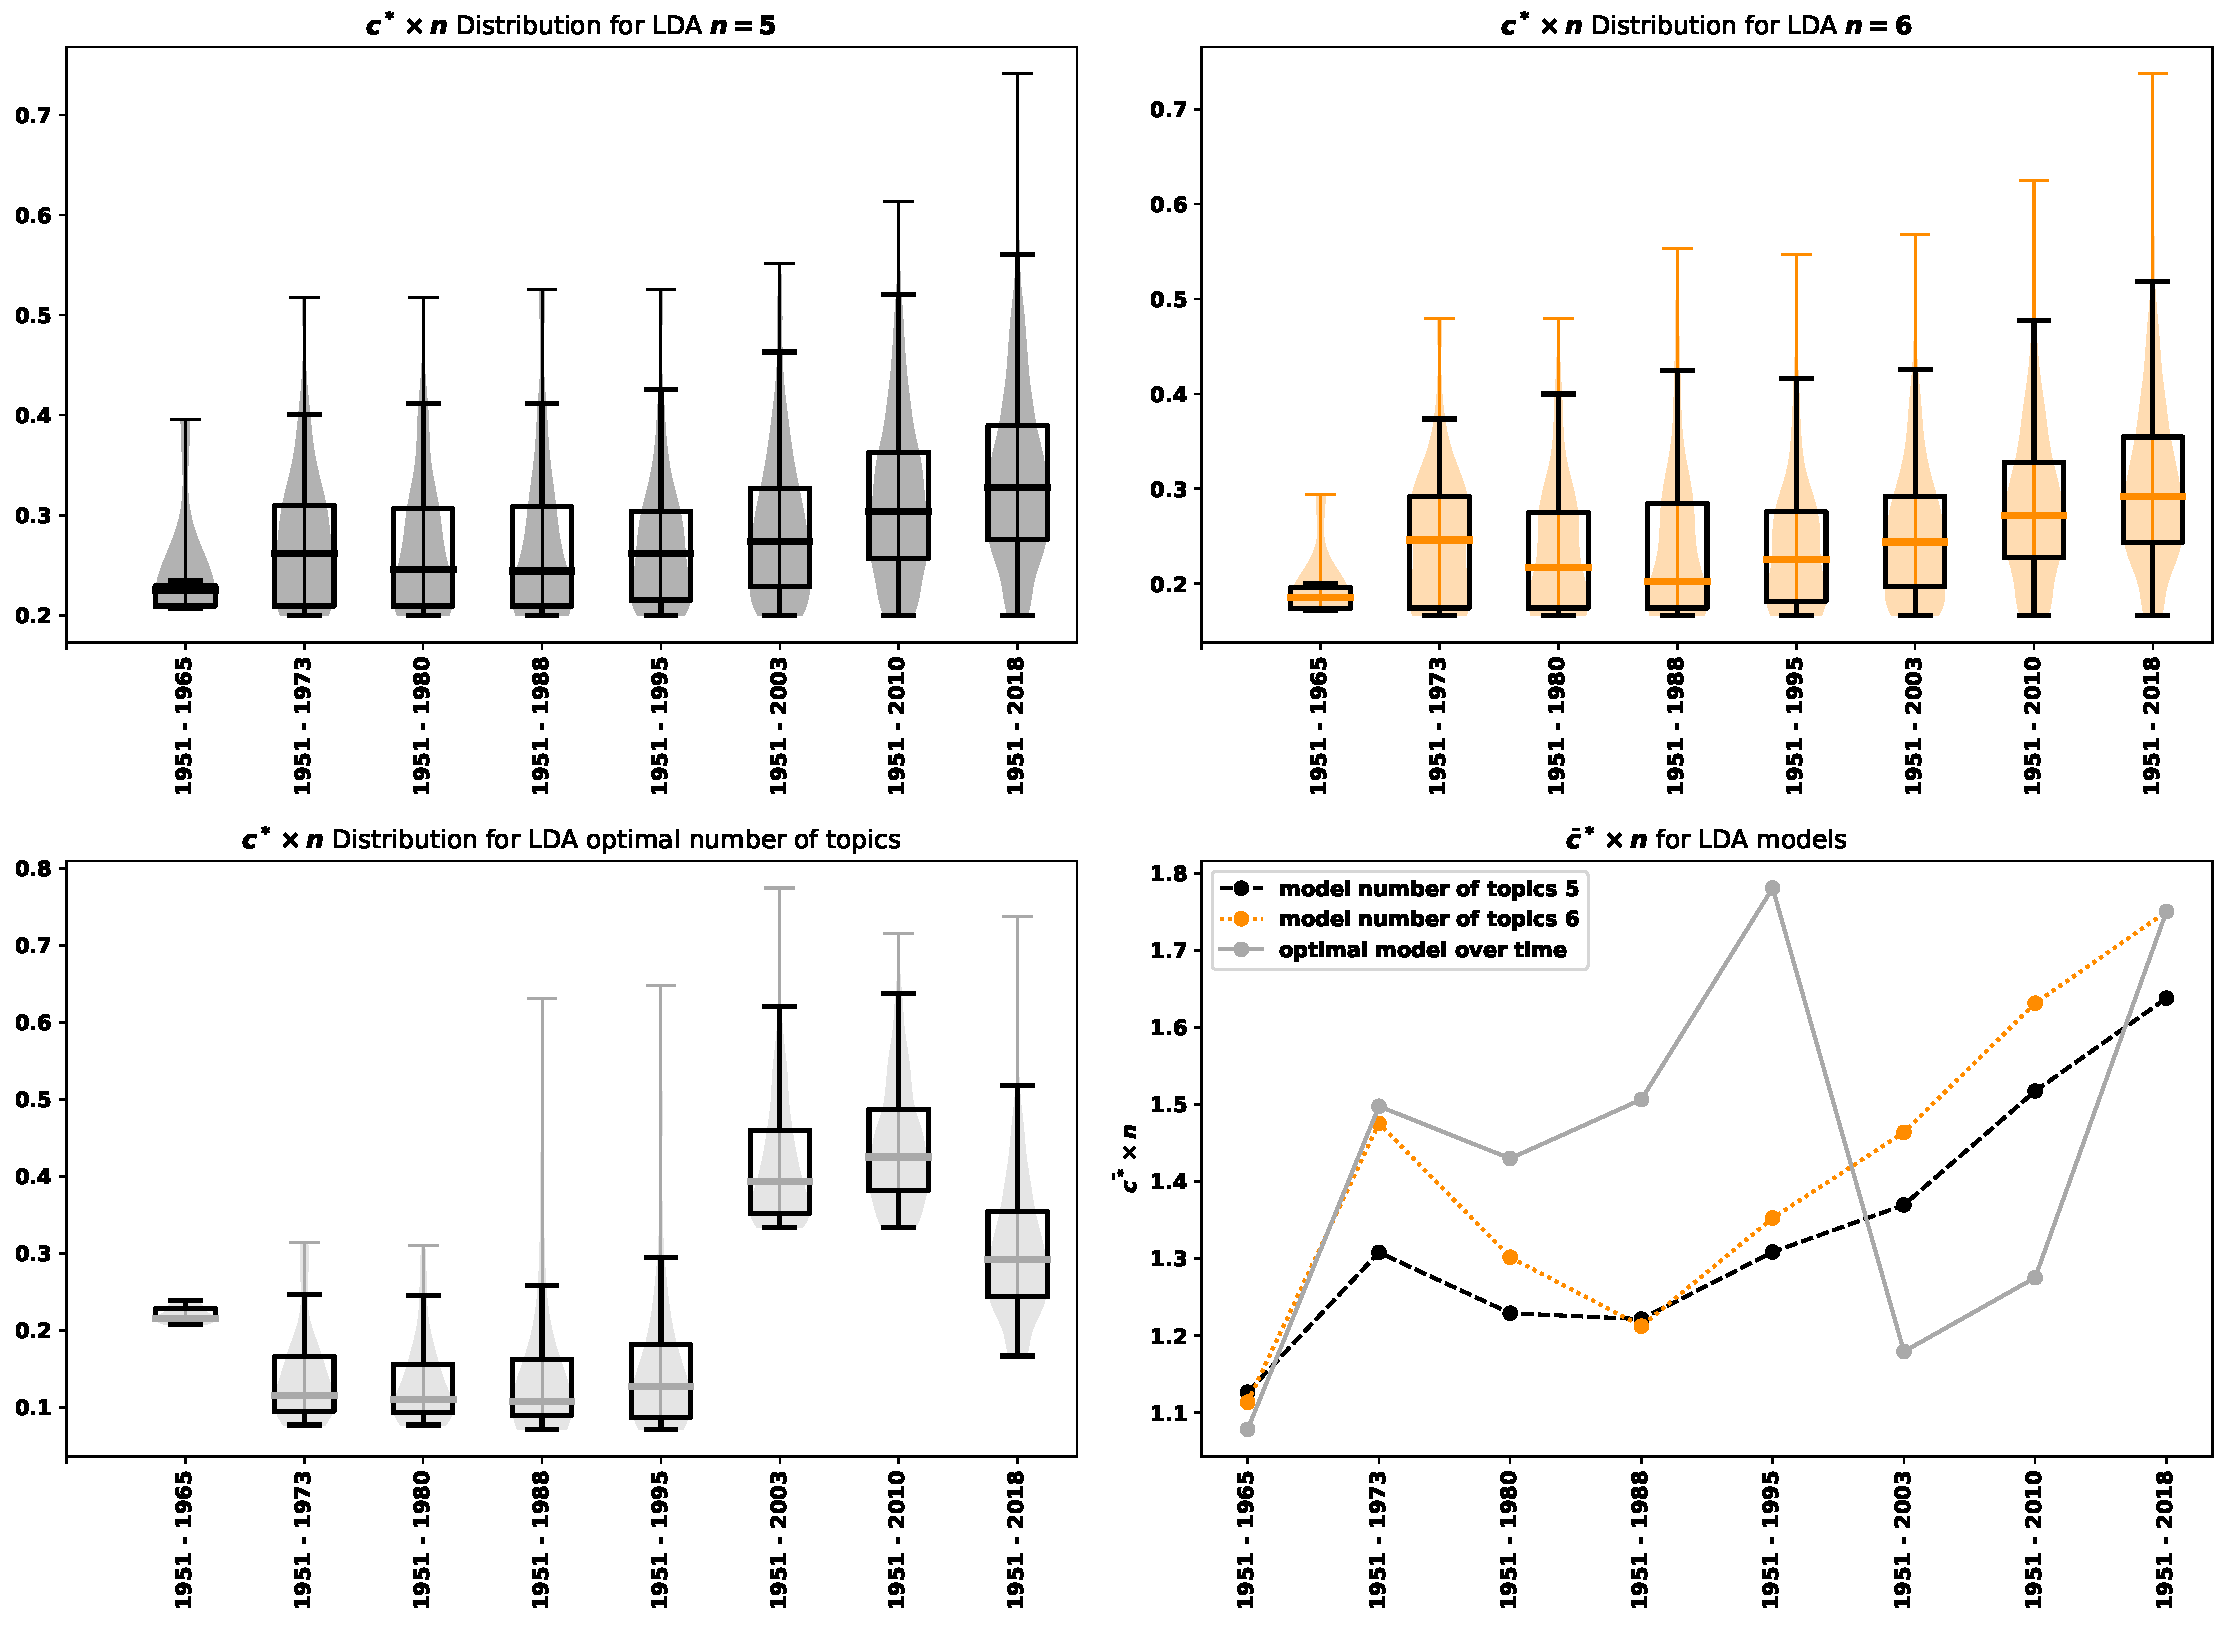
\includegraphics[width=.75\textwidth]{src/chapters/chapters-03/paper/Literature-Article/assets/images/contribution_over_time.pdf}
    \caption{Maximum percentage contributions (\(c^*\)) over the time periods,
    for the LDA models for the entire data set for \(n\) equal to 5, 6
    and the optimal number of topics over time.}
    \label{fig:median_percentage_contribution_over_time}
\end{figure}

In the following section the collaborative behaviour of authors in the field,
and within the field's topics as were presented in this section, are explored
using a network theoretic approach.

\section{Analysis of co-authorship network}\label{section:co_authorship}

The collaborative behaviour of authors in the field of the PD is assessed using
the co-authorship network, which as mentioned in
Section~\ref{section:methodology} is denoted as \(G\). There are a total of
\connectedcomponents connected components in \(G\) and the largest component has
a size of \largestcc nodes. The largest connected component is going to be
refereed to as the main cluster of the network and is denoted as \(\bar{G}\). A
graphical representation of both networks is shown in
Figure~\ref{fig:graphical_representation_graphs} and a metrics summary is given
by Table~\ref{table:network_comparison.tex}.

\begin{figure}[!hbtp]\vspace{-2cm}
    \begin{subfigure}{.95\textwidth}\centering
        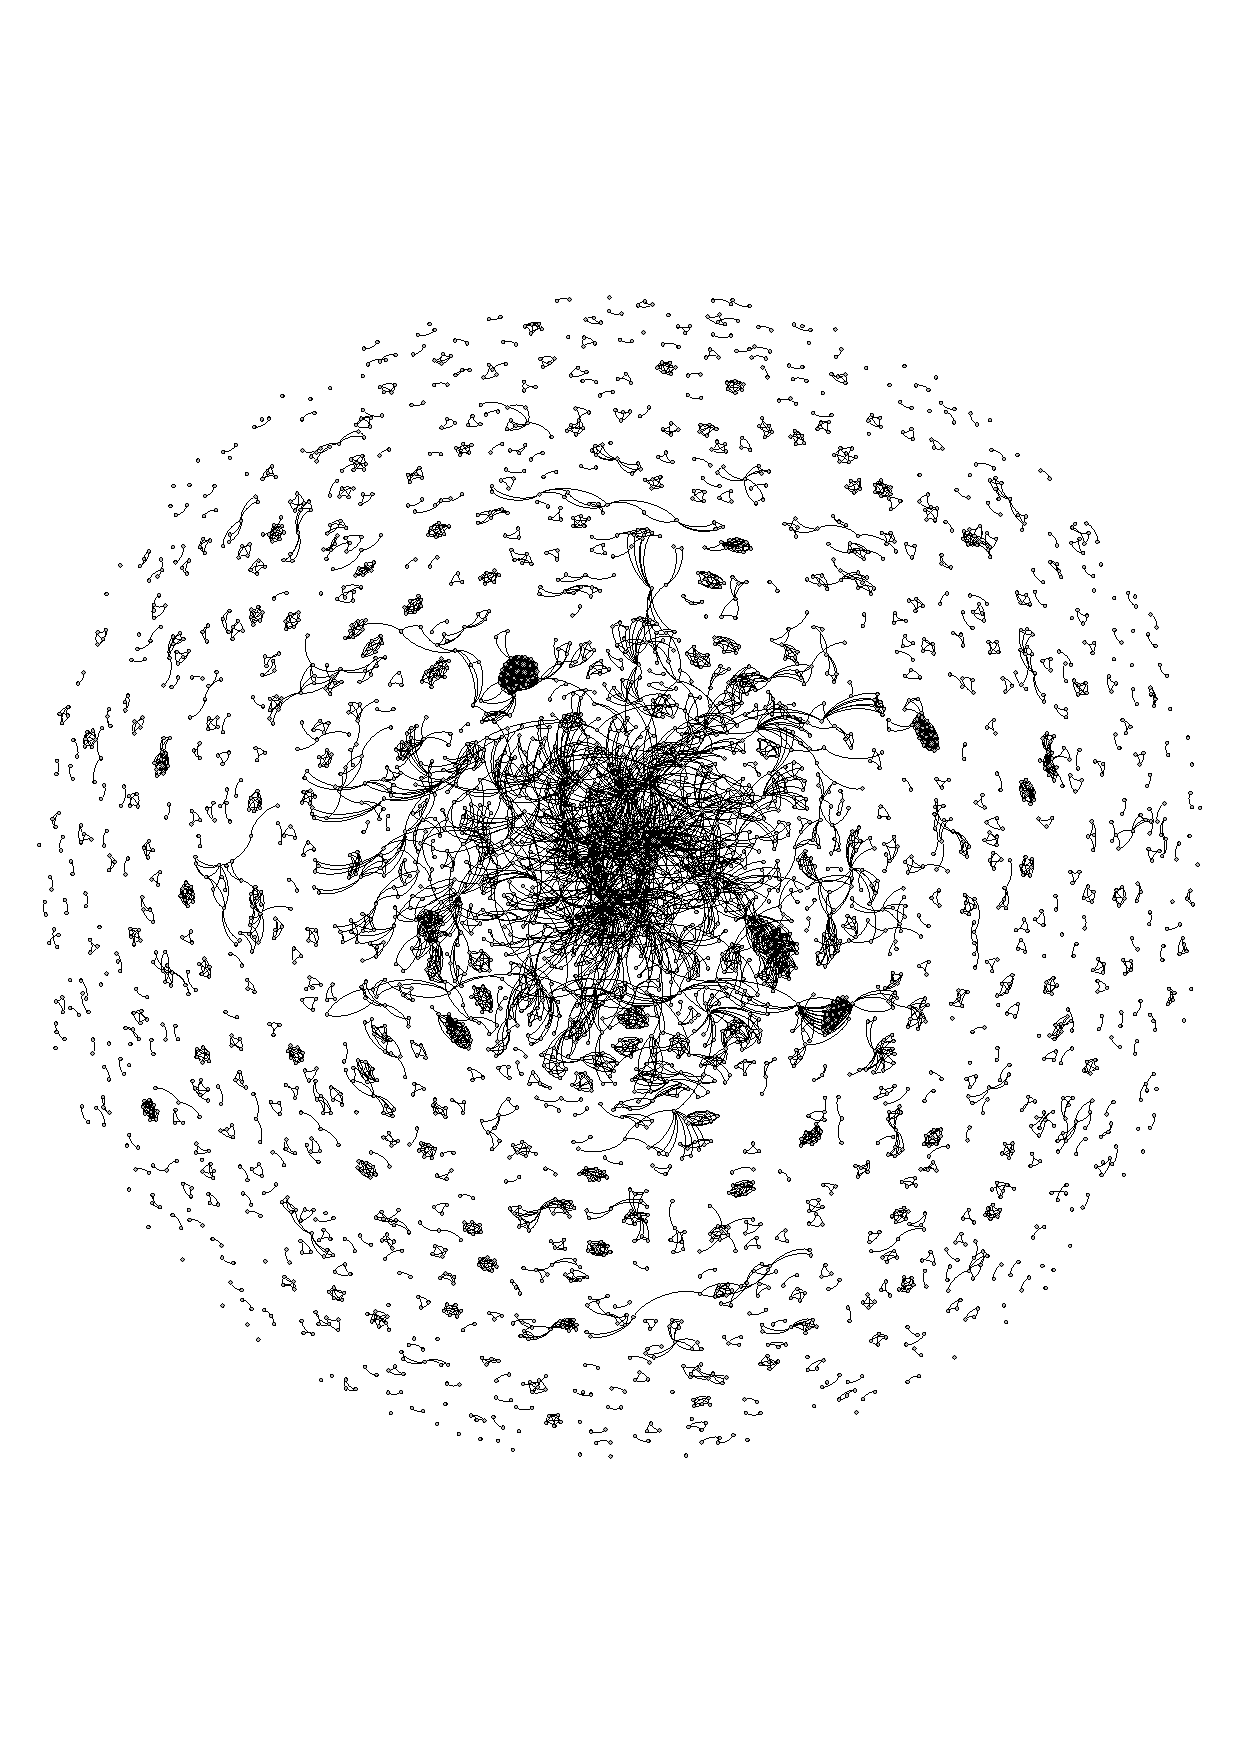
\includegraphics[width=.5\textwidth]{src/chapters/chapters-03/paper/Literature-Article/assets/images/pd_network.pdf}
        \caption{\(G\) the co-authorship network for the IPD.}
    \end{subfigure}\hfill
    \begin{subfigure}{.95\textwidth}\centering
        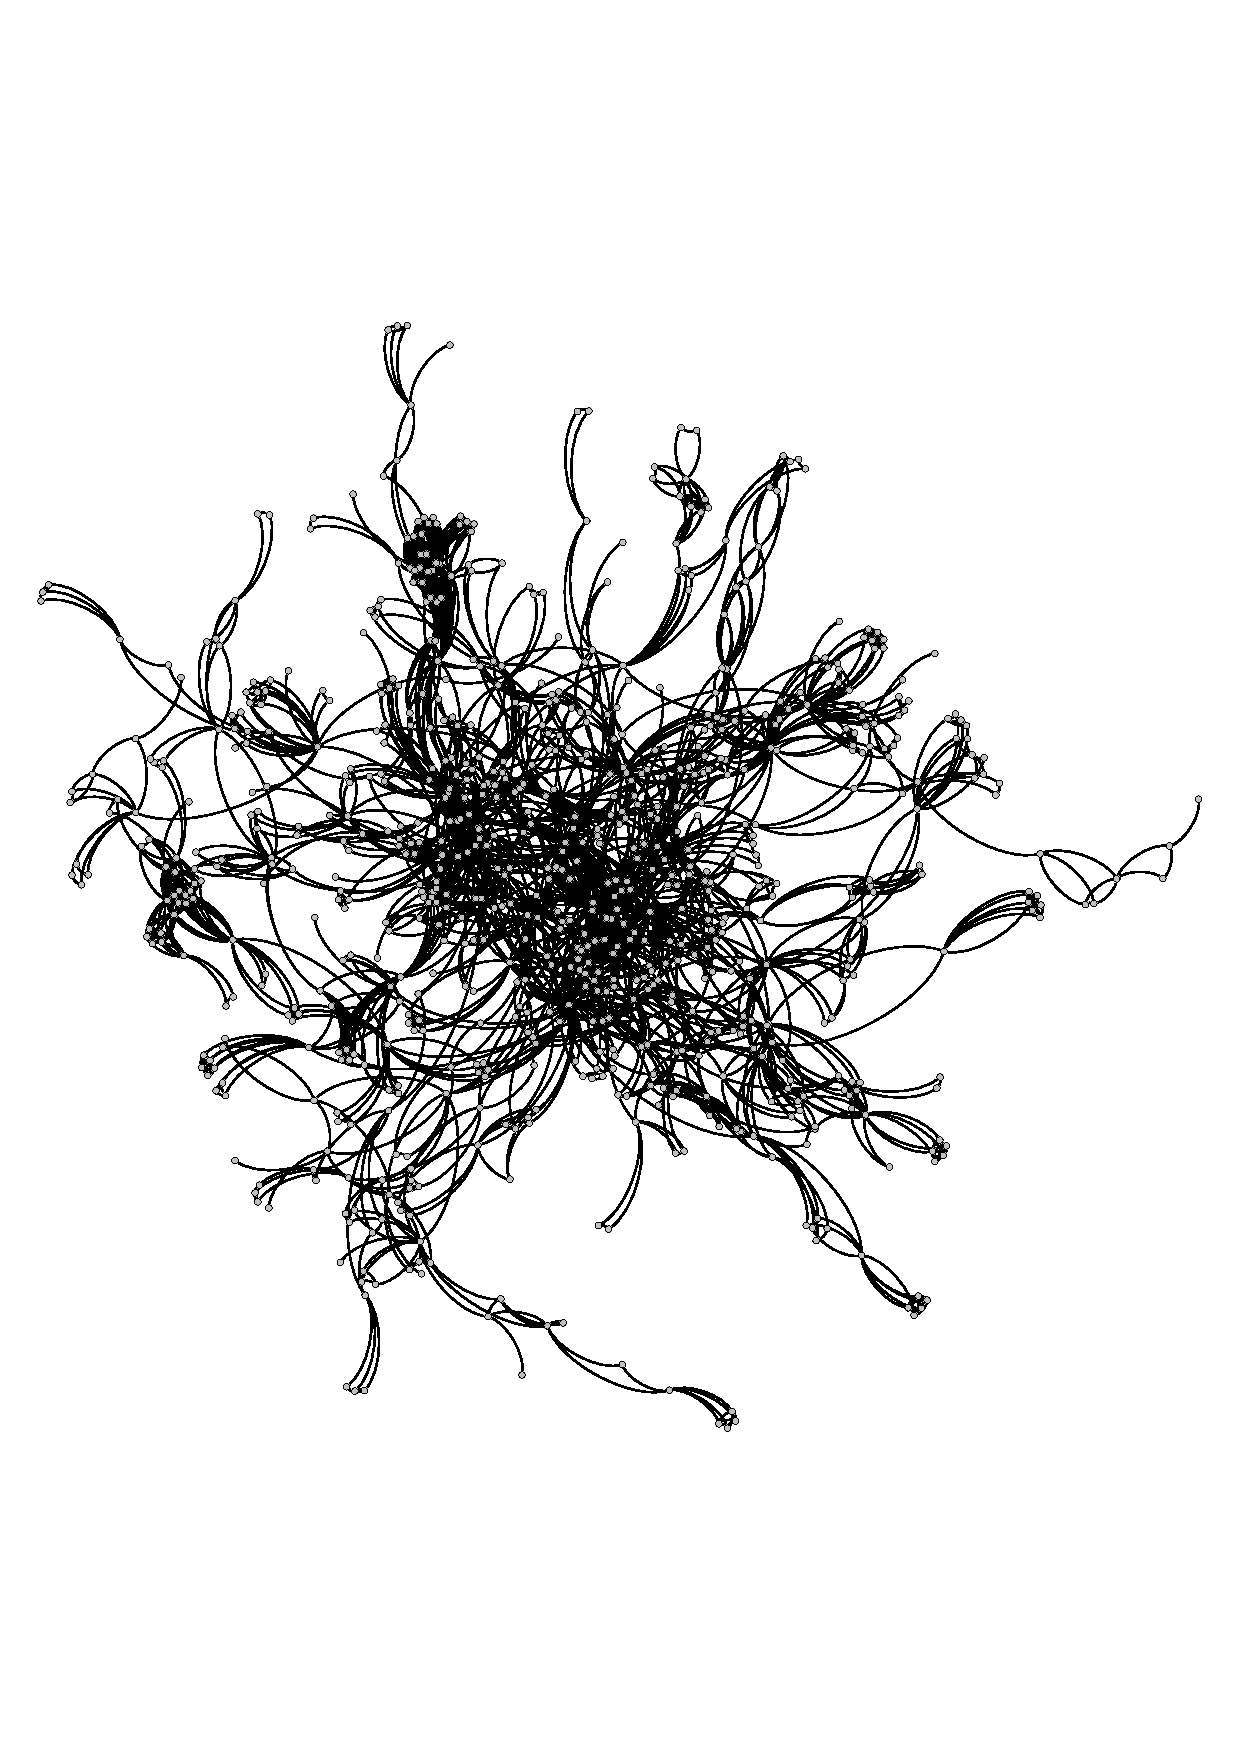
\includegraphics[width=.5\textwidth]{src/chapters/chapters-03/paper/Literature-Article/assets/images/pd_network_cluster.pdf}
        \caption{\(\bar{G}\) the largest connected component of \(G\).}
     \end{subfigure}
     \caption{A graphical representation of \(G\) and \(\bar{G}\)}\label{fig:graphical_representation_graphs}
\end{figure}

\textbf{Is the Prisoner's Dilemma a collaborative field?}

Based on Table~\ref{table:network_comparison.tex} an author in \(G\) has on
average 4 collaborators and a 70\% probability of collaborating with a
collaborator's co-author. An author of \(\bar{G}\) on average is 7\% more likely
to write with a collaborator's co-author and on average has 2 more
collaborators. Moreover, there are only \isolatedpercentage\% of authors in the
PD that has no connection to any other author.

How does this compare to other fields? Two more data sets for the topics
``Price of Anarchy'' and ``Auction Games'' have been collected in order to
compare the collaborative behaviour of the PD to other game theoretic fields. A
total of 3444 publications have been collected for Auction games and 748 for
Price of Anarchy. Price of Anarchy is relatively a new field, with the first
publication on the topic being~\cite{Koutsoupias1999} in 1999. This explains the
small number of articles that have been retrieved. Both data sets have been
archived and are available in~\cite{auction_data_2018, anarchy_data_2018}.
The networks for both data sets have been generated in the same way as \(G\).
A summary of the networks' metrics are given by Table~\ref{table:other_topics_network_comparison.tex}.

The average degrees for the Price of Anarchy and for Auction games are lower
than the PD's. In Auction games an author is more likely to have no collaborators,
and in the Price of Anarchy there are almost no authors that are not connected
to someone. This could be an effect of the field being introduced in more modern
days. Overall, an author in the PD has on average more collaborators
and there are less isolated authors compared to another well established game
theoretic field. These results seem to indicate that the PD is a \textit{relatively} collaborative
field.

However, both \(G\) and \(\bar{G}\) have a high modularity (larger than 0.84) and a large number of
communities (967 and 25 respectively). A high modularity implies that authors create their own publishing
communities but not many publications from authors from different communities
occur. Thus, author tends to collaborate with authors in their communities but
not many efforts are made to create new connections to other communities and
spread the knowledge of the field across academic teams. The fields
of both Price of Anarchy and Auction games also have high modularity, and
that could indicate that is in fact how academic publications are.

Thus, \textbf{the PD is indeed a collaborative field but perhaps it is not
more collaborative than other fields}, as there is no effort from the authors
to write with people outside their community.

\begin{table}[!hbtp]
    \centering
    \resizebox{\textwidth}{!}{
    \begin{tabular}{lrrrrrrrrrr}
\toprule
{} &  \# Nodes &  \# Edges  &  \% Isolated nodes &  \# Connected components &  Size of largest component &  Av. degree &  \# Communities &  Modularity &  Clustering coeff \\
\midrule
$G$       &     4011 &     7642 &               3.2 &                     947 &                        796 &       3.811 &            967 &     0.96491 &             0.701 \\
$\bar{G}$ &      796 &     2214 &               0.0 &                       1 &                        796 &       5.563 &             25 &     0.84406 &             0.773 \\
\bottomrule
\end{tabular}
}
    \caption{Network metrics for \(G\) and \(\bar{G}\) respectively.}
    \label{table:network_comparison.tex}
\end{table}

\begin{table}[!hbtp]
    \centering
    \resizebox{\textwidth}{!}{
    \begin{tabular}{lrrrrP{0.2\textwidth}P{0.2\textwidth}rrrrr}
\toprule
{} &  \# Nodes &  \# Edges &  \# Isolated nodes &  \% Isolated nodes &  \# Connected components &  Size of largest component &  Av. degree &  \# Communities &  Modularity &  Clustering coeff \\
\midrule
auction Games    &     5165 &     7861 &               256 &               5.0 &                    1272 &                       1348 &       3.044 &           1294 &       0.957 &             0.622 \\
price of Anarchy &     1155 &     1953 &                 4 &               0.3 &                     245 &                        222 &       3.382 &            253 &       0.965 &             0.712 \\
\bottomrule
\end{tabular}
}
    \caption{Network metrics for auction games and price of anarchy networks respectively.}
    \label{table:other_topics_network_comparison.tex}
\end{table}

The evolution of the networks was also explored over time by constructing the
network cumulatively over 51 periods. Except from the first period 1951-1966 the
rest of the periods have a yearly interval (data for the years 1975 and 1982
were not retrieved by the collection data process). The metrics of each sub
network are given in the Appendix~\ref{appendix:tables}.

The results, similarly to the results of~\cite{Liu2015}, confirm that the
networks grow over time and that the networks always had a high modularity.
Since the first publications authors tend to write with people from their
communities, and that is not an effect of a specific time period.

\textbf{Are some topics more collaborative than other?}

The networks corresponding to the topics of Section~\ref{section:preliminary} have
also been generated similarly to \(G\). Note that authors with publications in
more than one topic exist, and these authors are included in all the corresponding
networks. A metrics' summary for all five topic networks is given by Table
\ref{table:topics_networks}.

Topic B is the network with the highest average degree followed by Topic A. The
topic with the smallest average degree, 2.5, is Topic C. In topics A and B the
number of isolated nodes is very small \(less than (0.2)\) compared to Topic E where the
percentage of isolated nodes is approximately 6\%. Moreover, in topics C and E
an author is 10\% more likely to collaborate with a collaborator's co-author.
Thus, \textbf{topics ``human subject research'' and ``biological studies'' tend
to be more collaborative than the topic of ``strategies'', and an authors in
these are less likely to have at least one collaborator compared to the topic of
``modeling problems as a PD''}.

\textbf{``Evolutionary dynamics on networks'' also appear to be a collaborative topic}.
In fact the network of the topic  is a
sub graph of \(\bar{G}\), the main cluster of \(G\) and it will be demonstrated in the following section that
authors in this network are more like to gain from the influence of the network
compared to any other topic network.

\begin{table}[!hbtp]
    \centering
    \resizebox{\textwidth}{!}{
    \begin{tabular}{lrrrrrrrrrr}
\toprule
{} &  \# Nodes &  \# Edges &  \# Isolated nodes &  \% Isolated nodes &  \# Connected components &  Size of largest component &  Av. degree &  \# Communities &  Modularity &  Clustering coeff \\
\midrule
Topic A &     1124 &     2137 &                15 &               1.3 &                     264 &                         56 &       3.802 &            265 &       0.983 &             0.759 \\
Topic B &      695 &     1382 &                13 &               1.9 &                     157 &                         80 &       3.977 &            158 &       0.950 &             0.773 \\
Topic C &      900 &     1141 &                41 &               4.6 &                     281 &                         29 &       2.536 &            281 &       0.981 &             0.636 \\
Topic D &      880 &     1509 &                17 &               1.9 &                     174 &                        312 &       3.430 &            183 &       0.918 &             0.701 \\
Topic E &     1045 &     1964 &                59 &               5.6 &                     354 &                         31 &       3.759 &            354 &       0.926 &             0.664 \\
\bottomrule
\end{tabular}
}
    \caption{Network metrics for topic networks.}\label{table:topics_networks}
\end{table}

\textbf{Are there authors which benefit more from their position in the network?}

There are two centrality measures reported in this work, closeness and
betweenness centrality. Closeness centrality is a measure of how easy it is for
an author to contact others, and consequently affect them; influence them. Thus
closeness centrality here is a measure of influence. Betweenness centrality is a
measure of how many paths pass through a specific node, thus the amount of
information this person has access to. Betweenness centrality is used here as a
measure of how much an author gains from the field. All centrality measure can
have values ranging from 0 to 1. The influence and the amount of information
an author has access to are used to explore which authors benefit more
from their position.

For \(G\) and \(\bar{G}\) the most central authors based on closeness and
betweenness centralities are given by Table~\ref{table:central_authors}. The
most central authors in \(G\) and \(\bar{G}\) are the same. This implies that
the results on centrality heavily rely on the main cluster (as expected). Matjaz Perc is an
author with 83 publications in the data set and the most central authors based
on both centrality measures. The most central authors are fairly similar between
the two measures. The author that appear to be central based on one measure and
not the other are Martin Nowak, Franz Weissing, Jianye Hao, Angel Sanchez and
Valerio Capraro which have access to information due to their
positioning but do not influence the network as much, and the opposite is true
for Attila Szolnoki, Luo-Luo Jiang Sandro Meloni, Cheng-Yi Xia and Xiaojie Chen.

It is obvious that in \(G\) the centralities values are low which suggests
that in the PD authors do not benefit from their positions. This could be an
effect of information not flowing from one community to another as authors tend
to write with people from their communities. Nevertheless,
\textbf{there are authors that do benefit from their position, but these are
only the authors connected to the main cluster}.

\begin{table}[!hbtp]
    \begin{center}
    \resizebox{.9\textwidth}{!}{\begin{tabular}{lgrgr|grgr}
\toprule
& \multicolumn{4}{c}{$G$} & \multicolumn{4}{c}{$\bar{G}$} \\
\midrule
{} &             Name &  Betweenness &             Name &  Closeness &             Name &  Betweenness &             Name &  Closeness \\
\midrule
1  &      Matjaz Perc &        0.015 &      Matjaz Perc &      0.066 &      Matjaz Perc &        0.373 &      Matjaz Perc &      0.330 \\
2  &        Zhen Wang &        0.011 &        Long Wang &      0.060 &        Zhen Wang &        0.279 &        Long Wang &      0.301 \\
3  &        Long Wang &        0.007 &     Yamir Moreno &      0.059 &        Long Wang &        0.170 &     Yamir Moreno &      0.299 \\
4  &     Martin Nowak &        0.006 &  Attila Szolnoki &      0.059 &     Martin Nowak &        0.159 &  Attila Szolnoki &      0.297 \\
5  &    Angel Sanchez &        0.004 &        Zhen Wang &      0.059 &    Angel Sanchez &        0.114 &        Zhen Wang &      0.296 \\
6  &     Yamir Moreno &        0.004 &    Arne Traulsen &      0.056 &     Yamir Moreno &        0.110 &    Arne Traulsen &      0.281 \\
7  &    Arne Traulsen &        0.004 &    Luo-Luo Jiang &      0.055 &    Arne Traulsen &        0.107 &    Luo-Luo Jiang &      0.280 \\
8  &   Franz Weissing &        0.004 &    Sandro Meloni &      0.055 &   Franz Weissing &        0.101 &    Sandro Meloni &      0.278 \\
9  &       Jianye Hao &        0.004 &     Cheng-Yi Xia &      0.055 &       Jianye Hao &        0.094 &     Cheng-Yi Xia &      0.276 \\
10 &  Valerio Capraro &        0.004 &     Xiaojie Chen &      0.055 &  Valerio Capraro &        0.093 &     Xiaojie Chen &      0.276 \\
\bottomrule
\end{tabular}
}
\end{center}
\caption{10 most central authors based on betweenness and closeness centralities
for \(G\) and \(\bar{G}\).}\label{table:central_authors}
\end{table}

The centrality measures for the topic networks have also been estimated and are
given in
Tables~\ref{table:central_authors_bc_topics}-\ref{table:central_authors_cc_topics}.
If information was flowing between the communities of the research topics then
there would be an increase to the values of centralities for the sub networks.
However, the only topic where authors gain from their positions are the authors
of Topic D (topic on evolutionary dynamics on network). From the list of names it is obvious that these authors are
part of \(\bar{G}\), and that the network of Topic D is a sub network of \(\bar{G}\).
This confirms the results. The people benefiting from their position in the co-authorship networks
corresponding to research topics of the PD are only the people from the main
cluster of \(G\).

The fact that most authors of the main cluster are primarily publishing in
evolutionary dynamics on networks indicates that publishing in this specific
topic differs from the other topics covered in this manuscript. There appears to
be more collaboration and influence in the publications on evolutionary
dynamics and authors are more likely to gain from their position,
though it is not clear as to why.

\newcolumntype{g}{>{\columncolor{Gray}}l}
\begin{table}[!hbtp]
    \begin{center}
    \resizebox{.9\textwidth}{!}{\begin{tabular}{lggllggllgg}
\toprule
& \multicolumn{2}{g}{Topic A} & \multicolumn{2}{c}{Topic B} & \multicolumn{2}{g}{Topic C} & \multicolumn{2}{c}{Topic D} & \multicolumn{2}{g}{Topic E}\\
\midrule
{} &                 Name &  Betweeness &             Name &  Betweeness &             Name &  Betweeness &              Name &  Betweeness &                  Name &  Betweeness \\
\midrule
1  &           David Rand &       0.002 &        Long Wang &       0.006 &   Daniel Ashlock &       0.001 &       Matjaz Perc &       0.064 &             Zengru Di &         0.0 \\
2  &      Valerio Capraro &       0.001 &    Luo-Luo Jiang &       0.005 &      Matjaz Perc &       0.000 &     Luo-Luo Jiang &       0.037 &             Jian Yang &         0.0 \\
3  &        Angel Sanchez &       0.001 &     Martin Nowak &       0.004 &       Karl Tuyls &       0.000 &      Yamir Moreno &       0.031 &  Yevgeniy Vorobeychik &         0.0 \\
4  &              Feng Fu &       0.001 &      Matjaz Perc &       0.003 &  Philip Hingston &       0.000 &  Christoph Hauert &       0.027 &       Otavio Teixeira &         0.0 \\
5  &         Martin Nowak &       0.000 &  Attila Szolnoki &       0.003 &     Eun-Youn Kim &       0.000 &         Long Wang &       0.024 &      Roberto Oliveira &         0.0 \\
6  &  Nicholas Christakis &       0.000 &  Christian Hilbe &       0.002 &    Wendy Ashlock &       0.000 &         Zhen Wang &       0.024 &              M. Nowak &         0.0 \\
7  &   Pablo Branas-Garza &       0.000 &     Yamir Moreno &       0.002 &  Attila Szolnoki &       0.000 &      Han-Xin Yang &       0.023 &             M. Harper &         0.0 \\
8  &     Toshio Yamagishi &       0.000 &     Xiaojie Chen &       0.002 &       Seung Baek &       0.000 &      Martin Nowak &       0.020 &              Xiao Han &         0.0 \\
9  &         James Fowler &       0.000 &    Arne Traulsen &       0.002 &     Martin Nowak &       0.000 &     Angel Sanchez &       0.017 &            Zhesi Shen &         0.0 \\
10 &            Long Wang &       0.000 &        Zhen Wang &       0.002 &    Thore Graepel &       0.000 &       Zhihai Rong &       0.016 &           Wen-Xu Wang &         0.0 \\
\bottomrule
\end{tabular}
}
\end{center}
\caption{10 most central authors based on betweenness centrality
for topics' networks.}\label{table:central_authors_bc_topics}
\end{table}

\newcolumntype{g}{>{\columncolor{Gray}}l}
\begin{table}[!hbtp]
    \begin{center}
    \resizebox{.9\textwidth}{!}{\begin{tabular}{lggllggllgg}
\toprule
& \multicolumn{2}{g}{Topic A} & \multicolumn{2}{c}{Topic B} & \multicolumn{2}{g}{Topic C} & \multicolumn{2}{c}{Topic D} & \multicolumn{2}{g}{Topic E}\\
\midrule
{} &                 Name &  Closeness &               Name &  Closeness &                 Name &  Closeness &             Name &  Closeness &             Name &  Closeness \\
\midrule
1  &           David Rand &      0.027 &          Long Wang &      0.043 &           Karl Tuyls &      0.022 &      Matjaz Perc &      0.123 &  Stefanie Widder &      0.029 \\
2  &      Valerio Capraro &      0.023 &        Matjaz Perc &      0.041 &        Thore Graepel &      0.019 &        Zhen Wang &      0.109 &   Rosalind Allen &      0.029 \\
3  &       Jillian Jordan &      0.022 &    Attila Szolnoki &      0.040 &           Joel Leibo &      0.018 &        Long Wang &      0.107 &  Thomas Pfeiffer &      0.029 \\
4  &  Nicholas Christakis &      0.021 &       Martin Nowak &      0.040 &        Edward Hughes &      0.017 &     Yamir Moreno &      0.105 &    Thomas Curtis &      0.029 \\
5  &         James Fowler &      0.020 &  Olivier Tenaillon &      0.038 &     Matthew Phillips &      0.017 &    Luo-Luo Jiang &      0.104 &     Carsten Wiuf &      0.029 \\
6  &         Martin Nowak &      0.020 &       Xiaojie Chen &      0.038 &  Edgar Duenez-Guzman &      0.017 &  Attila Szolnoki &      0.103 &    William Sloan &      0.029 \\
7  &        Angel Sanchez &      0.019 &             Bin Wu &      0.038 &    Antonio Castaneda &      0.017 &     Gyorgy Szabo &      0.102 &     Otto Cordero &      0.029 \\
8  &    Gordon Kraft-Todd &      0.019 &      Yanling Zhang &      0.037 &         Iain Dunning &      0.017 &     Xiaojie Chen &      0.102 &        Sam Brown &      0.029 \\
9  &        Akihiro Nishi &      0.019 &            Feng Fu &      0.037 &             Tina Zhu &      0.017 &    Guangming Xie &      0.101 &     Babak Momeni &      0.029 \\
10 &        Anthony Evans &      0.019 &         David Rand &      0.037 &          Kevin Mckee &      0.017 &     Lucas Wardil &      0.101 &     Wenying Shou &      0.029 \\
\bottomrule
\end{tabular}
}
\end{center}
\caption{10 most central authors based on closeness centrality
for topics' networks.}\label{table:central_authors_cc_topics}
\end{table}

The distributions of both centrality measures for all the networks of this
work are given in the Appendix~\ref{appendix:distributions}.

\section{Conclusion}\label{section:conclusion}

This manuscript has explored the research topics in the publications of the
Iterated Prisoner's Dilemma, and moreover, the authors' collaborative behaviour
and their influence in the research field. This was achieved by
applying network theoretic approaches and a LDA algorithm to a total of 2422
publications. Both the software~\cite{nikoleta_2017} and the data~\cite{nikoleta_2017}
have been archived and are available to be used by other researchers. In
fact~\cite{nikoleta_2017} has been used by~\cite{brane} and~\cite{arcas_blog}.

The data collection and an introduction to the methodology used in this work
were covered in Section~\ref{section:methodology}.
Section~\ref{section:preliminary} covered an initial analysis of the data set
which demonstrated that the PD is a field that continues to attract academic
attention and publications. In Section~\ref{section:topics} LDA was
applied to the data set to identify topics on which researchers have been
publishing. The LDA analysis showed that the data could be classified into 5
topics associated with human subject research, biological studies, strategies,
evolutionary dynamics on networks and modeling
problems as a PD. These topics summarize the field of the PD well, as they
demonstrate its interdisciplinarity and applications to a variety of problems. A
temporal analysis explored how relevant these topics have been over the course
of time, and it revealed that even though there were not the necessarily always
the most discussed topics they were still being explored by researchers.

The collaborative behaviour of the field was explored in
Section~\ref{section:co_authorship} by constructing the co authorship network.
It was concluded that the field is a collaborative field, where authors are
likely to write with a collaborator's co-authors and on average an author has 4
co-authors, however it not necessarily more collaborative than other fields. The
authors tend to collaborate with authors from one community, but not many
authors are involved in multiple communities. This however
might be an effect of academic research, and it might not be true just for the
field of the PD. Exploring the influence of authors and their gain from being in
the network of the field demonstrated that authors do not gain much, and the
authors with influence are only the ones connected to the main cluster, to a
``main'' group of authors. This `main'' group of authors consists of authors
publishing in evolutionary dynamics on networks. Thus, an author would be aiming
to publish on this topic if they were interested in gaining from their position
in the publications of the PD.

The study of the PD is the study of cooperation and investigating
the cooperative behaviours of authors is what this work has aimed to achieve.
Interesting areas of future work would include extending this analysis to more
game theoretic sub fields, to evaluate whether the results remain the same.

% \section{Acknowledgements}

% A variety of software have been used in this work:

% \begin{itemize}
%     \item The Matplotlib library for visualisation~\cite{hunter2007matplotlib}.
%     \item The Numpy library for data manipulation~\cite{walt2011numpy}.
%     \item The Networkx~\cite{networkx} package for analysing networks.
%     \item Gephi~\cite{ICWSM09154} open source package for visualising networks.
%     \item The Gensim library for the topic modeling~\cite{rehurek_lrec}.
%     \item The louvain library for calculating the networks modularity \url{https://github.com/taynaud/python-louvain}.
% \end{itemize}

% \bibliographystyle{plain}
% \bibliography{bibliography.bib}

\section{Cumulative Networks Metrics}\label{appendix:tables}

\subsection{Collaborativeness metrics for cumulative graphs, \(\tilde{G} \subseteq G\)}
\begin{table}[!hbtp]
    \centering
    \resizebox{.8\textwidth}{!}{
    \begin{tabular}{lrrrrrrrrrr}
\toprule
Period &  \# Nodes &  \# Edges &  \% Isolated nodes &  \multicolumn{1}{p{3cm}}{\centering \# Connected components} &  \multicolumn{1}{p{3cm}}{\centering Size of largest component} &  Av. degree &  \# Communities &  Modularity &  Clustering coeff \\
\midrule
1951 - 1966 &        6 &        3 &    0.0 &                       3 &                          2 &       1.000 &              3 &       0.667 &             0.000 \\
1951 - 1967 &        8 &        4 &    0.0 &                       4 &                          2 &       1.000 &              4 &       0.750 &             0.000 \\
1951 - 1968 &       19 &       15 &    0.0 &                       8 &                          5 &       1.579 &              8 &       0.684 &             0.228 \\
1951 - 1969 &       20 &       17 &    0.0 &                       8 &                          6 &       1.700 &              8 &       0.630 &             0.250 \\
1951 - 1970 &       22 &       18 &    0.0 &                       9 &                          6 &       1.636 &              9 &       0.667 &             0.227 \\
1951 - 1971 &       33 &       28 &    0.0 &                      13 &                          6 &       1.697 &             13 &       0.827 &             0.424 \\
1951 - 1972 &       39 &       34 &    0.0 &                      15 &                          6 &       1.744 &             15 &       0.867 &             0.513 \\
1951 - 1973 &       42 &       35 &    2.4 &                      17 &                          6 &       1.667 &             17 &       0.873 &             0.476 \\
1951 - 1974 &       42 &       35 &    2.4 &                      17 &                          6 &       1.667 &             17 &       0.873 &             0.476 \\
1951 - 1976 &       42 &       35 &    2.4 &                      17 &                          6 &       1.667 &             17 &       0.873 &             0.476 \\
1951 - 1977 &       44 &       36 &    2.3 &                      18 &                          6 &       1.636 &             18 &       0.880 &             0.455 \\
1951 - 1978 &       44 &       36 &    2.3 &                      18 &                          6 &       1.636 &             18 &       0.880 &             0.455 \\
1951 - 1979 &       47 &       40 &    2.1 &                      18 &                          6 &       1.702 &             18 &       0.884 &             0.454 \\
1951 - 1980 &       47 &       40 &    2.1 &                      18 &                          6 &       1.702 &             18 &       0.884 &             0.454 \\
1951 - 1981 &       50 &       46 &    2.0 &                      18 &                          6 &       1.840 &             18 &       0.889 &             0.497 \\
1951 - 1983 &       51 &       46 &    3.9 &                      19 &                          6 &       1.804 &             19 &       0.889 &             0.487 \\
1951 - 1984 &       53 &       47 &    3.8 &                      20 &                          6 &       1.774 &             20 &       0.894 &             0.469 \\
1951 - 1985 &       53 &       47 &    3.8 &                      20 &                          6 &       1.774 &             20 &       0.894 &             0.469 \\
1951 - 1986 &       53 &       47 &    3.8 &                      20 &                          6 &       1.774 &             20 &       0.894 &             0.469 \\
1951 - 1987 &       56 &       48 &    5.4 &                      22 &                          6 &       1.714 &             22 &       0.898 &             0.443 \\
1951 - 1988 &       62 &       52 &    6.5 &                      25 &                          6 &       1.677 &             25 &       0.909 &             0.449 \\
1951 - 1989 &       75 &       62 &    6.7 &                      31 &                          6 &       1.653 &             31 &       0.926 &             0.424 \\
1951 - 1990 &       79 &       64 &    6.3 &                      33 &                          6 &       1.620 &             33 &       0.930 &             0.403 \\
1951 - 1991 &       87 &       69 &    6.9 &                      37 &                          6 &       1.586 &             37 &       0.937 &             0.400 \\
1951 - 1992 &       95 &       72 &   10.5 &                      42 &                          6 &       1.516 &             42 &       0.941 &             0.367 \\
1951 - 1993 &      106 &       81 &   11.3 &                      47 &                          6 &       1.528 &             47 &       0.947 &             0.366 \\
1951 - 1994 &      124 &       95 &   12.9 &                      56 &                          6 &       1.532 &             56 &       0.955 &             0.394 \\
1951 - 1995 &      135 &      102 &   12.6 &                      61 &                          6 &       1.511 &             61 &       0.960 &             0.384 \\
1951 - 1996 &      142 &      105 &   12.7 &                      65 &                          6 &       1.479 &             65 &       0.962 &             0.365 \\
1951 - 1997 &      155 &      115 &   12.9 &                      71 &                          6 &       1.484 &             71 &       0.966 &             0.392 \\
1951 - 1998 &      191 &      140 &   11.0 &                      87 &                          6 &       1.466 &             87 &       0.973 &             0.367 \\
1951 - 1999 &      221 &      169 &   11.3 &                      99 &                          6 &       1.529 &             99 &       0.977 &             0.397 \\
1951 - 2000 &      250 &      195 &   10.8 &                     110 &                          6 &       1.560 &            110 &       0.979 &             0.418 \\
1951 - 2001 &      287 &      235 &   10.5 &                     125 &                          7 &       1.638 &            125 &       0.977 &             0.419 \\
1951 - 2002 &      335 &      278 &   10.7 &                     146 &                          7 &       1.660 &            146 &       0.979 &             0.428 \\
1951 - 2003 &      381 &      310 &   10.5 &                     168 &                          7 &       1.627 &            168 &       0.982 &             0.413 \\
1951 - 2004 &      437 &      370 &    9.2 &                     185 &                         10 &       1.693 &            185 &       0.983 &             0.424 \\
1951 - 2005 &      532 &      476 &    7.7 &                     214 &                         19 &       1.789 &            214 &       0.985 &             0.458 \\
1951 - 2006 &      640 &      603 &    6.7 &                     246 &                         22 &       1.884 &            246 &       0.987 &             0.486 \\
1951 - 2007 &      793 &      877 &    5.8 &                     283 &                         25 &       2.212 &            283 &       0.985 &             0.532 \\
1951 - 2008 &      948 &     1170 &    5.3 &                     318 &                         33 &       2.468 &            319 &       0.985 &             0.558 \\
1951 - 2009 &     1108 &     1442 &    4.9 &                     356 &                         71 &       2.603 &            358 &       0.982 &             0.573 \\
1951 - 2010 &     1300 &     1936 &    5.1 &                     402 &                        133 &       2.978 &            405 &       0.965 &             0.592 \\
1951 - 2011 &     1560 &     2375 &    5.1 &                     472 &                        157 &       3.045 &            475 &       0.970 &             0.613 \\
1951 - 2012 &     1837 &     2865 &    4.4 &                     534 &                        209 &       3.119 &            537 &       0.969 &             0.634 \\
1951 - 2013 &     2149 &     3420 &    4.3 &                     603 &                        322 &       3.183 &            609 &       0.965 &             0.644 \\
1951 - 2014 &     2481 &     3971 &    4.2 &                     683 &                        399 &       3.201 &            694 &       0.962 &             0.658 \\
1951 - 2015 &     2938 &     4877 &    3.7 &                     765 &                        504 &       3.320 &            779 &       0.965 &             0.675 \\
1951 - 2016 &     3469 &     6532 &    3.3 &                     850 &                        613 &       3.766 &            863 &       0.964 &             0.696 \\
1951 - 2017 &     3735 &     7072 &    3.2 &                     895 &                        706 &       3.787 &            912 &       0.964 &             0.700 \\
1951 - 2018 &     4011 &     7642 &    3.2 &                     947 &                        796 &       3.811 &            967 &       0.966 &             0.701 \\
\bottomrule
\end{tabular}
}
\end{table}

\newpage

\subsection{Collaborativeness metrics for cumulative graphs' main clusters, \(\tilde{G} \subseteq \bar{G}\)}
\begin{table}[!hbtp]
    \centering
    \resizebox{.8\textwidth}{!}{
    \begin{tabular}{lrrrrrrrrrr}
\toprule
Periods &  \# Nodes &  \# Edges &  \# Isolated nodes &  \% Isolated nodes &  \# Connected components &  Size of largest component &  Av. degree &  \# Communities &  Modularity &  Clustering coeff \\
\midrule
1951 - 1966 &        2 &        1 &                 0 &               0.0 &                       1 &                          2 &       1.000 &              1 &       0.000 &             0.000 \\
1951 - 1967 &        2 &        1 &                 0 &               0.0 &                       1 &                          2 &       1.000 &              1 &       0.000 &             0.000 \\
1951 - 1968 &        5 &        8 &                 0 &               0.0 &                       1 &                          5 &       3.200 &              1 &       0.000 &             0.867 \\
1951 - 1969 &        6 &       10 &                 0 &               0.0 &                       1 &                          6 &       3.333 &              2 &       0.020 &             0.833 \\
1951 - 1970 &        6 &       10 &                 0 &               0.0 &                       1 &                          6 &       3.333 &              2 &       0.020 &             0.833 \\
1951 - 1971 &        6 &       10 &                 0 &               0.0 &                       1 &                          6 &       3.333 &              2 &       0.020 &             0.833 \\
1951 - 1972 &        6 &       10 &                 0 &               0.0 &                       1 &                          6 &       3.333 &              2 &       0.020 &             0.833 \\
1951 - 1973 &        6 &       10 &                 0 &               0.0 &                       1 &                          6 &       3.333 &              2 &       0.020 &             0.833 \\
1951 - 1974 &        6 &       10 &                 0 &               0.0 &                       1 &                          6 &       3.333 &              2 &       0.020 &             0.833 \\
1951 - 1976 &        6 &       10 &                 0 &               0.0 &                       1 &                          6 &       3.333 &              2 &       0.020 &             0.833 \\
1951 - 1977 &        6 &       10 &                 0 &               0.0 &                       1 &                          6 &       3.333 &              2 &       0.020 &             0.833 \\
1951 - 1978 &        6 &       10 &                 0 &               0.0 &                       1 &                          6 &       3.333 &              2 &       0.020 &             0.833 \\
1951 - 1979 &        6 &       10 &                 0 &               0.0 &                       1 &                          6 &       3.333 &              2 &       0.020 &             0.833 \\
1951 - 1980 &        6 &       10 &                 0 &               0.0 &                       1 &                          6 &       3.333 &              2 &       0.020 &             0.833 \\
1951 - 1981 &        6 &       10 &                 0 &               0.0 &                       1 &                          6 &       3.333 &              2 &       0.020 &             0.833 \\
1951 - 1983 &        6 &       10 &                 0 &               0.0 &                       1 &                          6 &       3.333 &              2 &       0.020 &             0.833 \\
1951 - 1984 &        6 &       10 &                 0 &               0.0 &                       1 &                          6 &       3.333 &              2 &       0.020 &             0.833 \\
1951 - 1985 &        6 &       10 &                 0 &               0.0 &                       1 &                          6 &       3.333 &              2 &       0.020 &             0.833 \\
1951 - 1986 &        6 &       10 &                 0 &               0.0 &                       1 &                          6 &       3.333 &              2 &       0.020 &             0.833 \\
1951 - 1987 &        6 &       10 &                 0 &               0.0 &                       1 &                          6 &       3.333 &              2 &       0.020 &             0.833 \\
1951 - 1988 &        6 &       10 &                 0 &               0.0 &                       1 &                          6 &       3.333 &              2 &       0.020 &             0.833 \\
1951 - 1989 &        6 &       10 &                 0 &               0.0 &                       1 &                          6 &       3.333 &              2 &       0.020 &             0.833 \\
1951 - 1990 &        6 &       10 &                 0 &               0.0 &                       1 &                          6 &       3.333 &              2 &       0.020 &             0.833 \\
1951 - 1991 &        6 &       10 &                 0 &               0.0 &                       1 &                          6 &       3.333 &              2 &       0.020 &             0.833 \\
1951 - 1992 &        6 &       10 &                 0 &               0.0 &                       1 &                          6 &       3.333 &              2 &       0.020 &             0.833 \\
1951 - 1993 &        6 &       10 &                 0 &               0.0 &                       1 &                          6 &       3.333 &              2 &       0.020 &             0.833 \\
1951 - 1994 &        6 &       10 &                 0 &               0.0 &                       1 &                          6 &       3.333 &              2 &       0.020 &             0.833 \\
1951 - 1995 &        6 &       10 &                 0 &               0.0 &                       1 &                          6 &       3.333 &              2 &       0.020 &             0.833 \\
1951 - 1996 &        6 &       10 &                 0 &               0.0 &                       1 &                          6 &       3.333 &              2 &       0.020 &             0.833 \\
1951 - 1997 &        6 &       10 &                 0 &               0.0 &                       1 &                          6 &       3.333 &              2 &       0.020 &             0.833 \\
1951 - 1998 &        6 &       10 &                 0 &               0.0 &                       1 &                          6 &       3.333 &              2 &       0.020 &             0.833 \\
1951 - 1999 &        6 &       10 &                 0 &               0.0 &                       1 &                          6 &       3.333 &              2 &       0.020 &             0.833 \\
1951 - 2000 &        6 &       10 &                 0 &               0.0 &                       1 &                          6 &       3.333 &              2 &       0.020 &             0.833 \\
1951 - 2001 &        7 &       21 &                 0 &               0.0 &                       1 &                          7 &       6.000 &              1 &       0.000 &             1.000 \\
1951 - 2002 &        7 &       21 &                 0 &               0.0 &                       1 &                          7 &       6.000 &              1 &       0.000 &             1.000 \\
1951 - 2003 &        7 &       21 &                 0 &               0.0 &                       1 &                          7 &       6.000 &              1 &       0.000 &             1.000 \\
1951 - 2004 &       10 &       13 &                 0 &               0.0 &                       1 &                         10 &       2.600 &              2 &       0.376 &             0.553 \\
1951 - 2005 &       19 &       28 &                 0 &               0.0 &                       1 &                         19 &       2.947 &              3 &       0.544 &             0.730 \\
1951 - 2006 &       22 &       35 &                 0 &               0.0 &                       1 &                         22 &       3.182 &              4 &       0.527 &             0.720 \\
1951 - 2007 &       25 &       39 &                 0 &               0.0 &                       1 &                         25 &       3.120 &              5 &       0.558 &             0.686 \\
1951 - 2008 &       33 &       62 &                 0 &               0.0 &                       1 &                         33 &       3.758 &              4 &       0.623 &             0.736 \\
1951 - 2009 &       71 &      148 &                 0 &               0.0 &                       1 &                         71 &       4.169 &              6 &       0.697 &             0.698 \\
1951 - 2010 &      133 &      387 &                 0 &               0.0 &                       1 &                        133 &       5.820 &              7 &       0.726 &             0.749 \\
1951 - 2011 &      157 &      465 &                 0 &               0.0 &                       1 &                        157 &       5.924 &              8 &       0.727 &             0.725 \\
1951 - 2012 &      209 &      611 &                 0 &               0.0 &                       1 &                        209 &       5.847 &             11 &       0.733 &             0.737 \\
1951 - 2013 &      322 &      892 &                 0 &               0.0 &                       1 &                        322 &       5.540 &             12 &       0.780 &             0.743 \\
1951 - 2014 &      399 &     1109 &                 0 &               0.0 &                       1 &                        399 &       5.559 &             15 &       0.794 &             0.742 \\
1951 - 2015 &      504 &     1368 &                 0 &               0.0 &                       1 &                        504 &       5.429 &             24 &       0.811 &             0.751 \\
1951 - 2016 &      613 &     1677 &                 0 &               0.0 &                       1 &                        613 &       5.471 &             21 &       0.819 &             0.761 \\
1951 - 2017 &      706 &     1935 &                 0 &               0.0 &                       1 &                        706 &       5.482 &             29 &       0.830 &             0.772 \\
1951 - 2018 &      796 &     2214 &                 0 &               0.0 &                       1 &                        796 &       5.563 &             25 &       0.845 &             0.773 \\
\bottomrule
\end{tabular}
}
\end{table}


\section{Centrality Measures Distributions}

\subsection{Distrubutions for \(G\) and \(\bar{G}\)}

\begin{figure}[!hbtp]
    \centering
    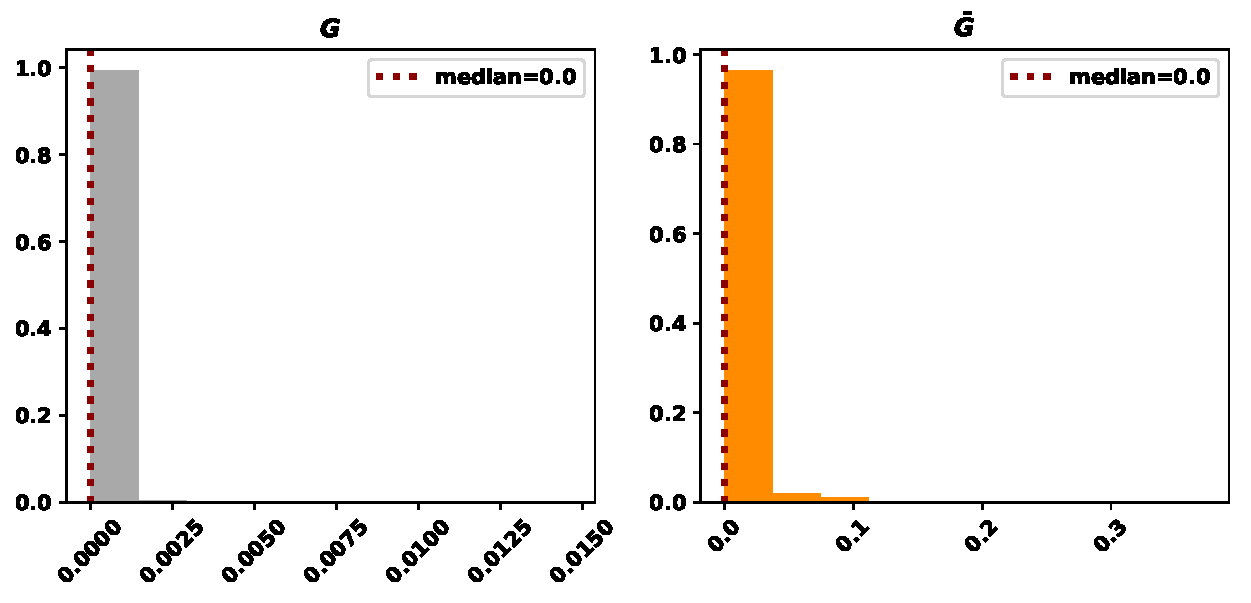
\includegraphics[width=.8\textwidth]{src/chapters/chapters-03/paper/Literature-Article/assets/images/pd_betweeness_centralities.pdf}
    \caption{Distributions of betweenness centrality in \(G\) and \(\bar{G}\)}
    \label{fig:bc_distributions}
\end{figure}

\begin{figure}[!hbtp]
    \centering
    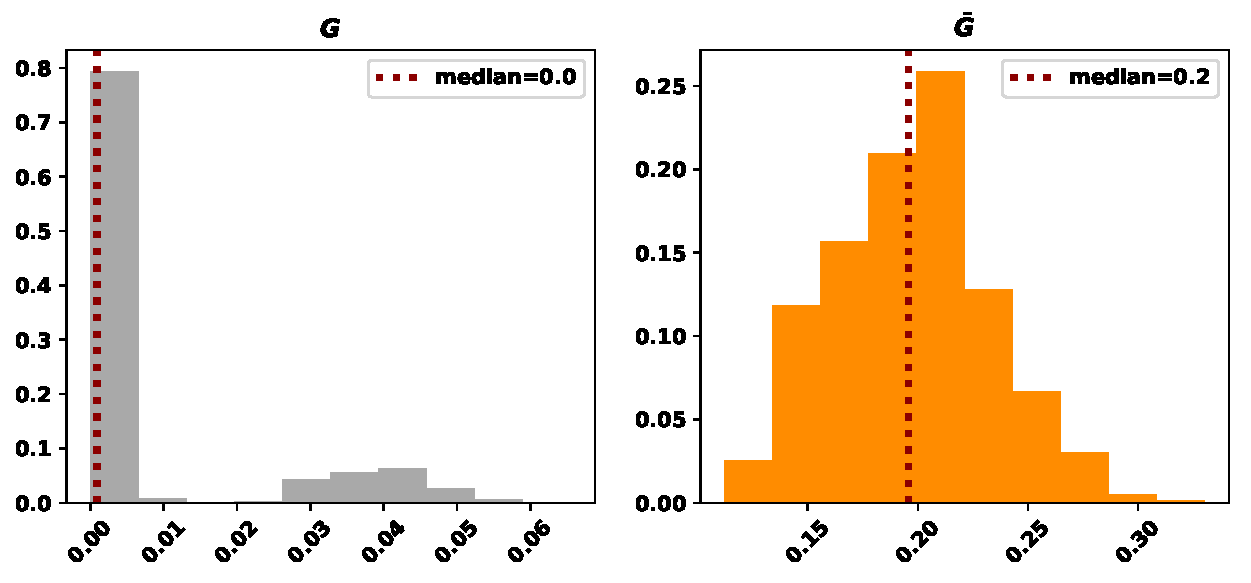
\includegraphics[width=.8\textwidth]{src/chapters/chapters-03/paper/Literature-Article/assets/images/pd_closeness_centralities.pdf}
    \caption{Distributions of closeness centrality in \(G\) and \(\bar{G}\)}
    \label{fig:cc_distributions}
\end{figure}

\subsection{Distrubutions for Topic Networks}\label{appendix:distributions}

\begin{figure}[!hbtp]
    \centering
    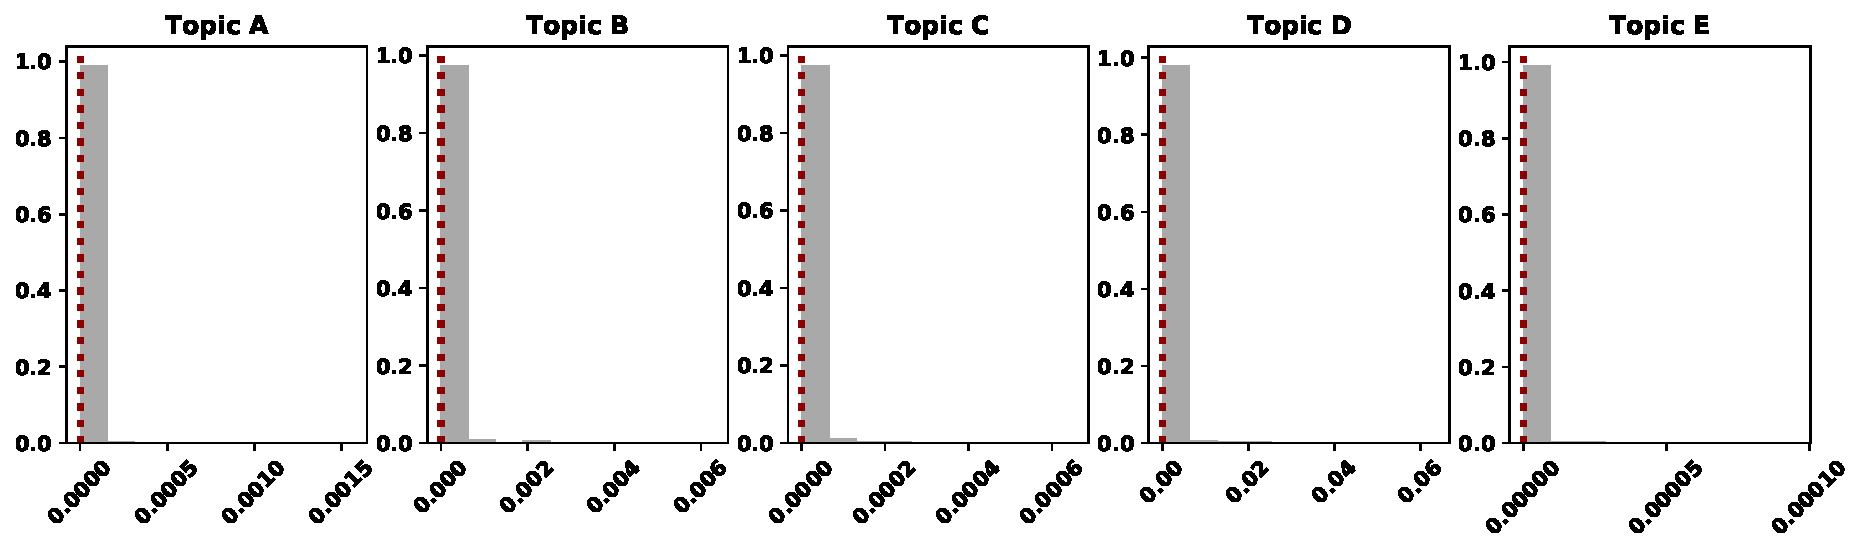
\includegraphics[width=\textwidth]{src/chapters/chapters-03/paper/Literature-Article/assets/images/topics_betweeness_distributions.pdf}
    \caption{Distributions of betweenness centrality in topics' networks.}
    \label{fig:bc_distributions_topics}
\end{figure}

\begin{figure}[!hbtp]
    \centering
    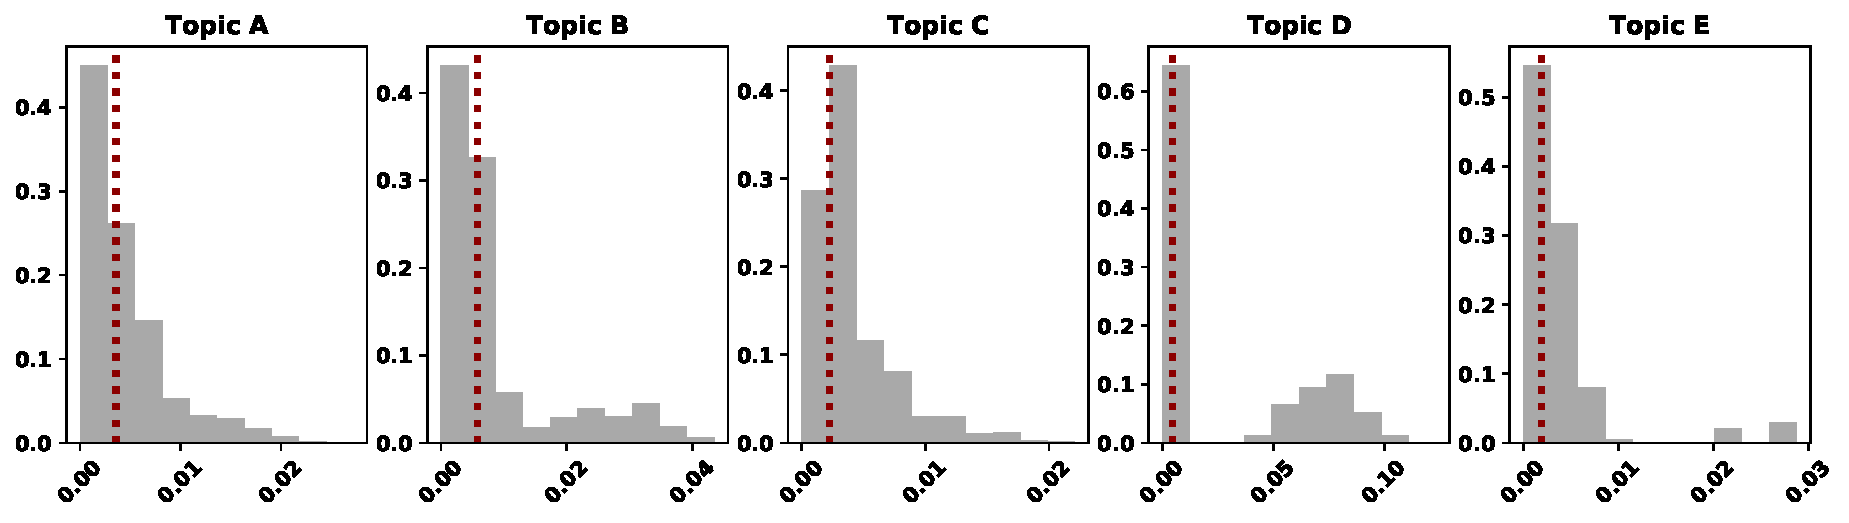
\includegraphics[width=\textwidth]{src/chapters/chapters-03/paper/Literature-Article/assets/images/topics_closeness_distributions.pdf}
    \caption{Distributions of closeness centrality in topics' networks.}
    \label{fig:cc_distributions_topics}
\end{figure}

\chapter{A meta analysis of tournaments and an evaluation of performance in the
Iterated Prisoner's Dilemma.}

The Iterated Prisoner's Dilemma has been used for decades as a model of
behavioural interactions. From the celebrated performance of Tit for Tat, to the
introduction of the zero-determinant strategies, to the use of sophisticated
structures such as neural networks, the literature has been exploring the
performance of strategies in the game for years. The results of the literature,
however, have been relying on the performance of specific strategies in a finite
number of tournaments, whereas this manuscript evaluates
\numberofstrategies strategies' effectiveness in more than 40000 tournaments.
The top ranked strategies are presented, and moreover, the impact of features on
their success are analysed using machine learning techniques. The analysis
determines that the cooperating ratio of a
strategy in a given tournament compared to the mean and median cooperator is the
most important feature. The conclusions are distinct for different types of
tournaments. For instance a strategy with a theory of mind would aim to be the mean/median
cooperator in standard tournaments, whereas in tournaments with probabilistic
ending it would aim to cooperate 10\% of the times the median cooperator did.

\section{Background}

The Iterated Prisoner's Dilemma (IPD) is a repeated two player game that models
behavioural interactions, and more specifically, interactions where
self-interest clashes with collective interest. At each turn of the game both
players, simultaneously and independently, decide between cooperation (C) and
defection (D) whilst having memory of their prior interactions. The payoffs for each
player, at each turn, is influenced by their own choice and the choice of the
other player. The payoffs of the game are generally defined by:

\[\begin{pmatrix}
R & S \\
T & P
\end{pmatrix}\]

where \(T > R > P > S\) and \(2R > T + S\). The most common values used in
the literature~\cite{Axelrod1981} are $R=3, P=1, T=5, S=0$. These values are also
used in this work.

Conceptualising strategies and understanding the best way of playing the game
has been of interest to the scientific community since the formulation of the
game in 1950~\cite{Flood1958}. Following the computer tournaments of Axelrod in the
1980's~\cite{Axelrod1980a, Axelrod1980b}, a strategy's performance in a round
robin computer tournament became a common evaluation technique for newly designed
strategies. Today more than 200 strategies exist in the literature and several
tournaments, excluding Axelrod's, have been undertaken~\cite{Bendor1991,
Harper2017, Kendall2007, Stephens2002, Stewart2012}.

In the 80's, Axelrod performed two computer tournaments~\cite{Axelrod1980a,
Axelrod1980b}. The contestants were strategies submitted in the form of computer
code. They competed against all other entries, a copy of themselves and a random
strategy. The winner was decided on the average score a strategy achieved. The
winner of both tournaments was the simple strategy Tit For Tat which cooperated
on the first turn and then simply copied the previous action of it's opponent.
Due to the strategy's strong performance in both tournaments, and moreover in a
series of evolutionary experiments~\cite{Axelrod1981}, Tit For Tat was thought
to be the most robust basic strategy in the IPD.

However, further research proved that the strategy had weakness, and more
specifically, it was shown that the strategy suffered in environments with
noise~\cite{Bendor1991, Donninger1986, Molander1985, Hammerstein1984}. This was
mainly due to the strategy's lack of generosity and contrition. The strategy was
quick to punish a defection, and in a noisy environment it could lead to a
repeated cycle of defections and cooperations. Some new strategies, more
robust in tournaments with noise, were soon introduced and became the new
protagonists of the game. These include Nice and Forgiving~\cite{Bendor1991},
Pavlov~\cite{Nowak1993} and Generous Tit For Tat~\cite{Nowak1992}.

In 2004, a $20^{\text{th}}$ Anniversary Iterated Prisoner Dilemma Tournament
took place with 233 entries. This time the winning strategy was not designed on
a reciprocity based approach but on a mechanism of
teams~\cite{J.P.Delahaye1993Lp, J.P.Delahaye1995LIeP, A.Rogers2007Ctpw}. A team
from Southampton University took advantage of the fact that a participant was
allowed to submit multiple strategies. They submitted a total of 60 strategies
that could recognised each other and colluded to increase one members score.
This resulted with three of the strategies to be ranked in the top spots. The
performance of the Southampton University team received mixed attention, though
they had won the tournament as stated in~\cite{us_blog} "technically this
strategy violates the spirit of the Prisoner's Dilemma, which assumes that the
two prisoners cannot communicate with one another".

Another set of IPD strategies that have received a lot of attention
are the zero-determinant strategies (ZDs)~\cite{Press2012}. By
forcing a linear relationship between the payoffs ZDs can ensure that they will
never receive less than their opponents. The
American Mathematical Society's news section stated that ``the world of game
theory is currently on fire''.
ZDs are indeed a set of mathematically unique strategies
and robust in pairwise interactions, however, their simplicity and extortionate
behaviour have been tested. In~\cite{Harper2017} a tournament containing over
200 strategies, including ZDs, was ran and none of them
ranked in top spots. Instead, the top ranked strategies were a set of
trained strategies based on lookup tables~\cite{Axelrod1987}, hidden markov
models~\cite{Harper2017} and finite state automata~\cite{Miller1996}.

Though only a select pieces of work have been discussed, the IPD literature is
rich, and new strategies and competitions are being published every year. The
question, however, still remains the same: what is the best way to play the
game? Compared to other works, whereas a few selected strategies are evaluated
on a small number of tournaments, this manuscript evaluates the performance of \numberofstrategies
strategies in \numberofalltournaments tournaments. These tournaments do not
consist by just standard round robin tournaments, but also by tournaments with noise
and tournaments with a probabilistic ending. The later part of the paper, evaluates
the impact of features on the performance of the strategies using modern
machine learning techniques. These features include measures regarding a
strategy's behaviour and measures regarding the tournaments. The data set used
in this work has been made publicly available~\cite{data} and can be used
for further analysis and insights.

The different tournament types as well as the data collection, which is made
possible due an open source package called Axelrod-Python~\cite{axelrodproject},
are covered in Section~\ref{section:data_collection}.
Section~\ref{section:top_performances}, focuses on the best performing
strategies for each type of tournament and overall.
Section~\ref{section:evaluation_of_performance}, explores the traits which
contribute to good performance, and finally the results are summarised in
Section~\ref{section:conclusion}. This manuscripts uses several parameters.
These are introduced in the following sections, however, the full set of
parameters and their definitions are given in Appendix~\ref{app:parameters}.

\section{Data collection}\label{section:data_collection}

For the purposes of this manuscript a data set containing results of IPD
tournaments has been generated and is available at~\cite{data}. This was done using the
open source package Axelrod-Python~\cite{axelrodproject}, and more specifically,
version 3.0.0. Axelrod-Python allows for different types of IPD computer
tournaments to be simulated whilst containing a list of over 180 strategies.
Most of these are strategies described in the literature with a few exceptions
being strategies that have been contributed specifically to the package. This
paper make use of \numberofstrategies strategies implemented in version 3.0.0. A
list of the strategies is given in the Appendix~\ref{app:list_of_players}.
Though Axelrod-Python features several tournament types, this work considers
only standard, noisy, probabilistic ending and noisy probabilistic ending
tournaments.

\textbf{Standard tournaments}, are tournaments similar to that of Axelrod's
in~\cite{Axelrod1980a}. There are \(N\) strategies which all play an iterated
game of \(n\) number of turns against each other. Note that self interactions
are not included. Similarly, \textbf{noisy
tournaments} have \(N\) strategies and \(n\) number of turns, but at each turn
there is a probability \(p_n\) that a player's action will be flipped.
\textbf{Probabilistic ending tournaments}, are of size \(N\) and after each turn
a match between strategies ends with a given probability \(p_e\). Finally,
\textbf{noisy probabilistic ending} tournaments have both a noise probability
\(p_n\) and an ending probability \(p_e\). For smoothing the simulated results a
tournament is repeated for \(k\) number of times. This was allowed to vary 
in order to evaluate the effect of smoothing. The winner of each tournament
is based on the average score a strategy achieved and not by the number of wins.

The process of collecting tournament results implemented in this manuscript is described by
Algorithm~\ref{algorithm:data_generation}. For each trial a random size \(N\) is
selected, and from the \numberofstrategies strategies a random list of \(N\) strategies is
chosen. For the given list of strategies a standard, a noisy, a probabilistic
ending and a noisy probabilistic ending tournament are performed and repeated
\(k\) times. The parameters for the tournaments, as well as the number of
repetitions, are selected once for each trial. The parameters and their
respective minimum and maximum values are given by
Table~\ref{table:parameters_values}.

\begin{table}[!htbp]
    \begin{center}
        \resizebox{.6\textwidth}{!}{
        \begin{tabular}{lcccc}
    \toprule
    parameter & parameter explanation &   min value & max value \\
    \midrule
    $N$ & number of strategies  & 3 & 195 \\
    $k$ & number of repetitions  & 10 & 100 \\
    $n$ & number of turns      & 1 & 200 \\
    $p_n$ & probability of flipping action at each turn  & 0 & 1   \\
    $p_e$ & probability of match ending in the next turn & 0 & 1   \\
    \bottomrule
        \end{tabular}}
    \end{center}
    \caption{Data collection; parameters' values}
    \label{table:parameters_values}
\end{table}

The source code for the data collection, as well as the source code for
the analysis, which will be discussed in the following sections, have been written
following best practices~\cite{Aberdour2007, Benureau2018}. It has been packaged
and is available here. %TODO archive code

\begin{algorithm}[!htbp]
    \setstretch{1.35}
    \ForEach{\text{seed} $\in [0, 11420]$}{
        $N \gets \text{randomly select integer}\in [N_{min}, N_{max}]$\;
        $\text{players} \gets  \text{randomly select $N$ players}$\;
        $k \gets  \text{randomly select integer}\in [k_{min}, k_{max}]$\;
        $n \gets  \text{randomly select integer}\in [n_{min}, n_{max}]$\;
        $p_n \gets  \text{randomly select float}\in [p_{n\, min}, p_{n\, max}]$\;
        $p_e \gets   \text{randomly select float}\in [p_{e\, min}, p_{e\, max}]$\;
        \vspace{0.4cm}
        $\text{result standard}$ $\gets$ Axelrod.tournament$(\text{players}, n, k)$\;
        $\text{result noisy}$ $\gets$ Axelrod.tournament$(\text{players}, n, p_n, k)$\;
        $\text{result probabilistic ending}$ $\gets$ Axelrod.tournament$(\text{players}, p_e, k)$\;
        $\text{result noisy probabilistic ending}$ $\gets$ Axelrod.tournament$(\text{players}, p_n, p_e, k)$\;

    }
    \KwRet{result standard, result noisy, result probabilistic ending,
    result noisy probabilistic ending}\;
    \caption{Data collection Algorithm}
    \label{algorithm:data_generation}
\end{algorithm}

A total of \uniquenumberofseeds trials of Algorithm~\ref{algorithm:data_generation} have been
run. For each trial the results for 4 different tournaments were collected,
thus a total of \numberofalltournaments $(\uniquenumberofseeds \times 4)$ tournament results have been
retrieved. Each tournament outputs a result summary in the form of
Table~\ref{table:output_result}. Each strategy have participated on average in
5154 tournaments of each type. The strategy with the maximum participation in each
tournament type is Inverse Punisher with 5639 entries. The strategy with the
minimum entries is EvolvedLookerUp 1 1 1 which was selected in 4693 trials.

The result summary, Table~\ref{table:output_result}, has \(N\) number of rows
because each row contains information for each strategy that participated in the
tournament. The information includes the strategy's rank, median score, the rate
with which the strategy cooperated $(C_r)$, its match win count and the
probability that the strategy cooperated in the opening move. Moreover, the
probabilities of a strategy being in any of the four states ($CC, CD, DC, DD$),
and the rate of which the strategy cooperated after each state. A measure that
has been manually included is the \textbf{normalised rank}. The normalised rank,
denoted as $r$, is calculated as a strategy's rank divided by the tournament's
size ($N$). In the next section the performance of these strategies is evaluated
based on their normalised rank.

\newcolumntype{g}{>{\columncolor{Gray}}c}
\begin{table}[!htbp]
    \begin{center}
    \resizebox{\textwidth}{!}{
    \begin{tabular}{ccccccgcgcgcgcg}
    \toprule 
    & & & & & &   \multicolumn{8}{g}{Rates}  \\
    Rank & Name & Median score & Cooperation rating $(C_r)$ & Win & Initial C &
    CC & CD & DC & DD & CC to C & CD to C & DC to C & DD to C \\
    0 &  EvolvedLookerUp2 2 2 & 2.97 & 0.705 & 28.0 & 1.0 & 0.639 & 0.066 & 0.189 &
    0.106 & 0.836 & 0.481 & 0.568 & 0.8 \\
    1 &  Evolved FSM 16 Noise 05 & 2.875 & 0.697 & 21.0 & 1.0 & 0.676 & 
    0.020 & 0.135 & 0.168 & 0.985 & 0.571 & 0.392 & 0.07 \\
    2 & PSO Gambler 1 1 1 & 2.874 & 0.684 &  23.0 &     1.0 &    0.651 &    0.034 &    0.152 &    0.164
    & 1.000 & 0.283 & 0.000 & 0.136 \\
    3 &  PSO Gambler Mem1 &  2.861 &        0.706 &  23.0 &      1.0 &    0.663
    &    0.042 &    0.145 &    0.150 &  1.000 &  0.510 &  0.000 &  0.122 \\
    4 &          Winner12 &  2.835 &        0.682 &  20.0 &      1.0 &
    0.651 &    0.031 &    0.141 &    0.177 &  1.000 &  0.441 &  0.000 &  0.462 \\
    $\dots$ & $\dots$ & $\dots$ & $\dots$ & $\dots$ & $\dots$ & $\dots$ & $\dots$ &
    $\dots$ & $\dots$ & $\dots$ & $\dots$ & $\dots$ & $\dots$ \\
    \bottomrule
    \end{tabular}}
\end{center}
\caption{Output result of a single tournament.}\label{table:output_result}
\end{table}

\section{Top ranked strategies}\label{section:top_performances}

This section evaluates the performance of \numberofstrategies IPD strategies. The performance of
each strategy is evaluated in four tournament types, which were presented in Section
\ref{section:data_collection}, followed by an evaluation of their performance
over all the \numberofalltournaments simulated tournaments of this work.

Each strategy participated in multiple tournaments of the same type (on average 5154).
For example Tit For Tat has participated in a total of 5114
tournaments of each type. The strategy's normalised rank distribution in these
is given in Figure~\ref{fig:tit_for_tat_r_distribution}. A value of \(r =
0\) corresponds to a strategy winning the tournament where a value of
\(r = 1\) corresponds to the strategy coming last. Because of the strategies'
multiple entries their performance is evaluated based on the
\textbf{median normalised rank} denoted as \(\bar{r}\).

\begin{figure}[!htbp]
    \centering
    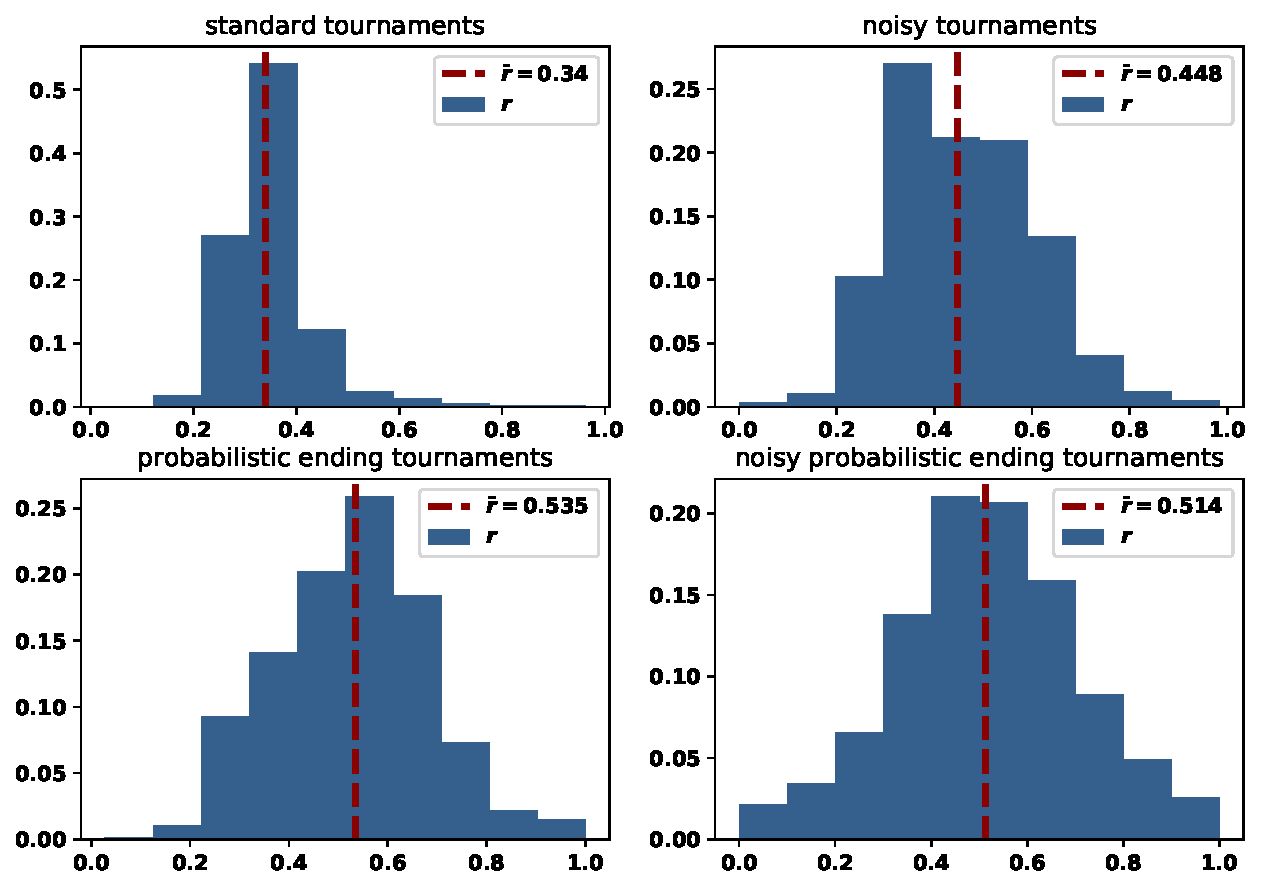
\includegraphics[width=.6\textwidth]{src/chapters/chapters-04/paper/axlml/images/tit_for_tat_r_distributions.pdf}
    \caption{Tit For Tat's $r$ distribution in tournaments. The best performance
    of the strategy has been in standard tournaments where it achieved a $\bar{r}$
    of 0.34.}
    \label{fig:tit_for_tat_r_distribution}
\end{figure}

The top 15 strategies for each tournament type based on \(\bar{r}\) are given in
Table~\ref{table:top_performances}.

\newcolumntype{g}{>{\columncolor{Gray}}l}
\begin{table}[!htbp]
    \begin{center}
    \resizebox{.9\textwidth}{!}{
        \begin{tabular}{lggllggllr}
\toprule
& \multicolumn{2}{g}{Standard} & \multicolumn{2}{c}{Noisy} & \multicolumn{2}{g}{Probabilistic ending} &  \multicolumn{2}{c}{Noisy probabilistic ending} \\
\midrule
& Name & $\bar{r}$ &                 Name & $\bar{r}$ &               Name & $\bar{r}$ &                 Name & $\bar{r}$ \\
\midrule
0  &            Evolved HMM 5 &   0.00667 &                 Grumpy &   0.14020 &          Fortress4 &   0.01266 &           Alternator &   0.30370 \\
1  &           Evolved FSM 16 &   0.00995 &                    $e$ &   0.19388 &           Defector &   0.01429 &               $\phi$ &   0.30978 \\
2  &     EvolvedLookerUp2 2 2 &   0.01064 &         Tit For 2 Tats &   0.20617 &  Better and Better &   0.01587 &                  $e$ &   0.31250 \\
3  &  Evolved FSM 16 Noise 05 &   0.01667 &  Slow Tit For Two Tats &   0.20962 &    Tricky Defector &   0.01875 &                $\pi$ &   0.31686 \\
4  &        PSO Gambler 2 2 2 &   0.02143 &           Cycle Hunter &   0.21538 &          Fortress3 &   0.02174 &    Limited Retaliate &   0.35263 \\
5  &              Evolved ANN &   0.02878 &         Risky QLearner &   0.22222 &     Gradual Killer &   0.02532 &     Anti Tit For Tat &   0.35431 \\
6  &            Evolved ANN 5 &   0.03390 &            Retaliate 3 &   0.22887 &         Aggravater &   0.02778 &          Retaliate 3 &   0.35563 \\
7  &        PSO Gambler 1 1 1 &   0.03704 &          Cycler CCCCCD &   0.23507 &             Raider &   0.03077 &  Limited Retaliate 3 &   0.35563 \\
8  &            Evolved FSM 4 &   0.04891 &            Retaliate 2 &   0.23913 &         Cycler DDC &   0.04545 &            Retaliate &   0.35714 \\
9  &         PSO Gambler Mem1 &   0.05036 &        Defector Hunter &   0.24038 &        Hard Prober &   0.05128 &          Retaliate 2 &   0.35767 \\
10 &                 Winner12 &   0.06011 &              Retaliate &   0.24177 &         SolutionB1 &   0.06024 &  Limited Retaliate 2 &   0.36134 \\
11 &             Fool Me Once &   0.06140 &    Hard Tit For 2 Tats &   0.25000 &      Meta Minority &   0.06077 &             Hopeless &   0.36842 \\
12 &                      DBS &   0.07143 &               ShortMem &   0.25286 &              Bully &   0.06081 &    Arrogant QLearner &   0.40651 \\
13 &            DoubleCrosser &   0.07200 &    Limited Retaliate 3 &   0.25316 &    Fool Me Forever &   0.07080 &    Cautious QLearner &   0.40909 \\
14 &              BackStabber &   0.07519 &      Limited Retaliate &   0.25706 &             EasyGo &   0.07101 &      Fool Me Forever &   0.41764 \\
\bottomrule
    \end{tabular}
    
    }
\end{center}
\caption{Top performances for each tournament type based on $\bar{r}$.}
\label{table:top_performances}
\end{table}

In standard tournaments 10 out of the 15 top strategies are introduced
in~\cite{Harper2017}. These are strategies based on finite state automata (FSM),
hidden markov models (HMM), artificial neural networks (ANN), lookup tables
(LookerUp) and stochastic lookup tables (Gambler) that have been trained using
reinforcement learning algorithms (evolutionary and particle swarm algorithms).
They have been trained to perform well against the strategies
in~\cite{axelrodproject} in a standard tournament, thus their performance in the
specific setting was anticipated. DoubleCrosser, and Fool Me Once, are
strategies not from the literature but from~\cite{axelrodproject}. DoubleCrosser
is a strategy that makes use of the number of turns because is set to defect on
the last two rounds. The strategy was expected to not perform as well in
tournaments where the number of turns is not specified, but the strategy did not
perform well in tournaments with noise either. Finally, Winner
12~\cite{mathieu2017} and DBS~\cite{Au2006} are both from the the literature.
DBS is strategy specifically designed for noisy environments, however, it ranks
highly only in standard ones.

Figure~\ref{fig:std_results} gives the distributions of $r$ for the top
ranked strategies. The distributions are skewed towards zero and the highest
median, of the top 15 strategies, is at 0.075. This indicates that the top ranked
strategies perform well in any given standard tournament, despite the opponents and
the number of turns.

\begin{figure}[!htbp]
    \centering
    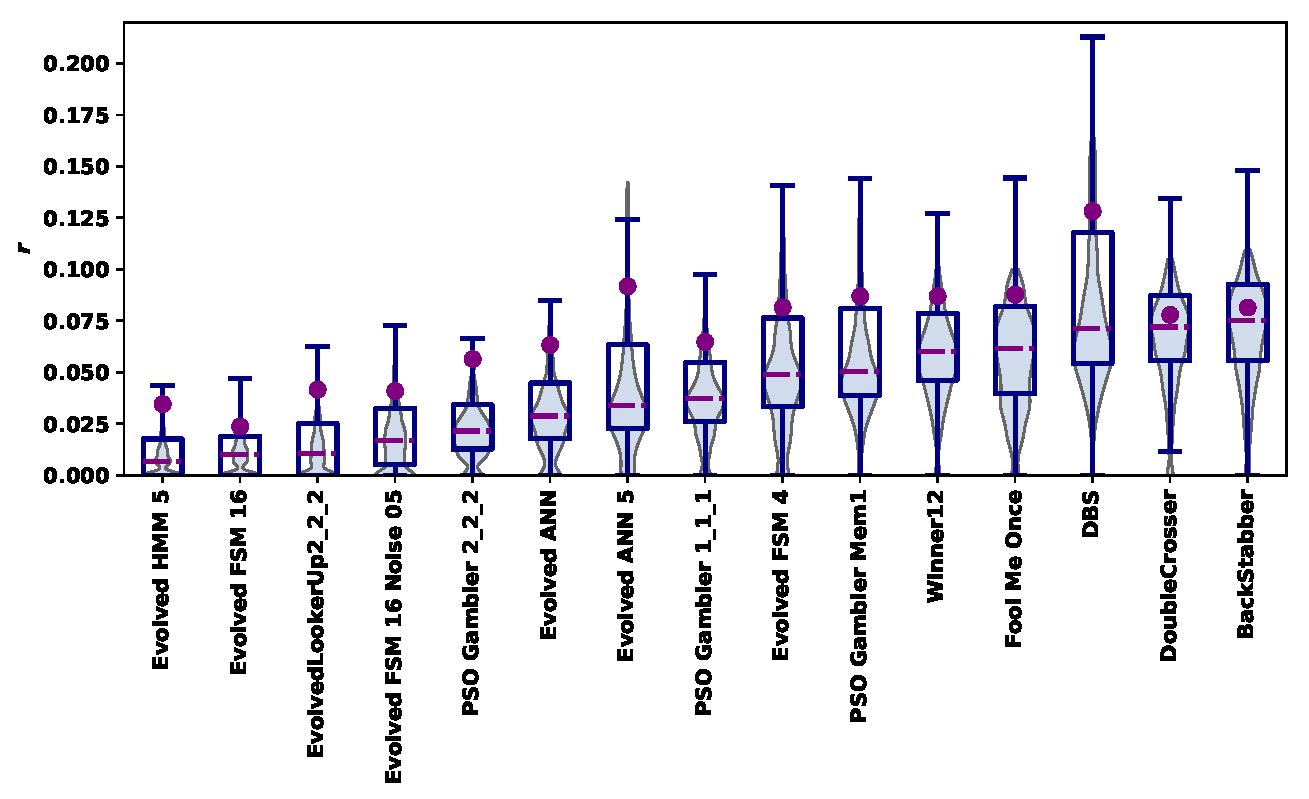
\includegraphics[width=.7\textwidth]{src/chapters/chapters-04/paper/axlml/images/performance_standard.pdf}
    \caption{$r$ distributions of top 15 strategies in standard tournaments.}\label{fig:std_results}
\end{figure}

The top strategies in noisy tournaments are shown in Figure~\ref{fig:noisy_results}. These include deterministic strategies, such
as Tit For 2 Tats~\cite{Axelrod1980b}, Slow Tit For Two Tats~\cite{axelrodproject}, Hard Tit For 2 Tats~\cite{Stewart2012}
and Cycler CCCCCD, and strategies which decide their actions based on the
cooperations to defections ratio, such as ShortMem~\cite{Carvalho2013}, Grumpy
and $e$~\cite{axelrodproject}. Slow Tit For Two Tats is the same strategy as 
Tit For 2 Tats, and at the time of writing this manuscript the
contributors of~\cite{axelrodproject} made a new release where the strategy
has been removed. However, for the purpose of this work the strategy is kept.
The Retaliate and
Limited Retaliate strategies are implemented in~\cite{axelrodproject} by the
same contributor. They are strategies designed to defect if the opponent has
tricked them more often than \(x\%\) of the times that they have
done the same. Finally, in $4^{\text{th}}$ and $9^{\text{th}}$ place are Hunter
strategies which trying to extort, equivalently, strategies that play cyclically
and defectors.

From Figure~\ref{fig:noisy_results}, it is evident that the normalised rank
distributions in noisy environments are more variant with higher medians
compared to standard tournaments. The distributions are bimodal. This indicates
that although the top ranked strategies mainly performed well, there are several
tournaments that they ranked in the bottom half. To gain a better understanding
of the behaviour in noisy tournaments, the \(r\) distributions for the top 6
of Figure~\ref{fig:noisy_results} strategies over the noise probability \(p_n\),
are given in Figure~\ref{fig:effect_of_noise}.

\begin{figure}[!htbp]
    \centering
    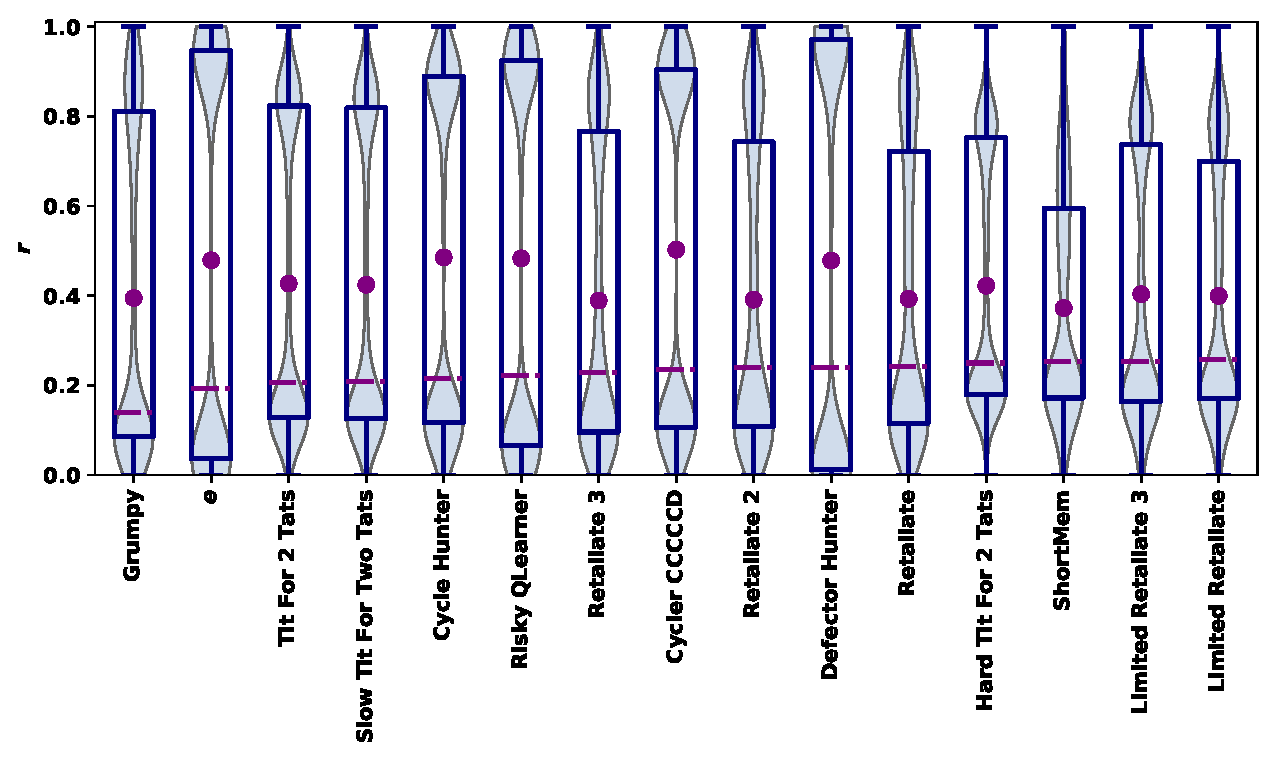
\includegraphics[width=.7\textwidth]{src/chapters/chapters-04/paper/axlml/images/performance_noise.pdf}
    \caption{\(r\) distributions for best performed strategies in noisy tournaments.}
    \label{fig:noisy_results}
\end{figure}

Figure~\ref{fig:effect_of_noise} shows that for \(p_n\) values lower than 0.5
Grumpy, Tit For 2 Tats and Slow Tit For Two Tat perform moderately, and \(e\),
Cycle Hunter and Ricky QLearner perform poorly. At \(p_n=0.5\) all the
distributions become bimodal. This is because with a noise probability of 0.5,
all strategies correspond to a random player. Interestedly, for a \(p_n\) larger
than 0.5 all of the 6 strategies become successful. Note that a value \(p_n=1\)
corresponds to a strategy playing opposite from what it intended to. Thus, it is
demonstrated that the successful strategies is noisy tournaments are sometimes
effective when \(p_n=0.5\) but overall they are very successful whn they are
playing opposite from their original design. If during the data collection a
\(p_n\) strictly less 0.5 was considered then the top ranked strategies would be
different. There are a total of 5661 trials where \(p_n<0.5\) and the top ranked
strategies are given in Table~\ref{table:subset_noise_result}. The median ranks
are lower than before and the top spots are mainly overtaken by Meta strategies
which include NMWE deterministic and NMWE Long Memory. The Meta
strategies~\cite{axelrodproject} create a team of strategies for themselves and
choose to play as a member of their team based on their scores against a given
opponent.

\begin{figure}[!htbp]
    \centering
    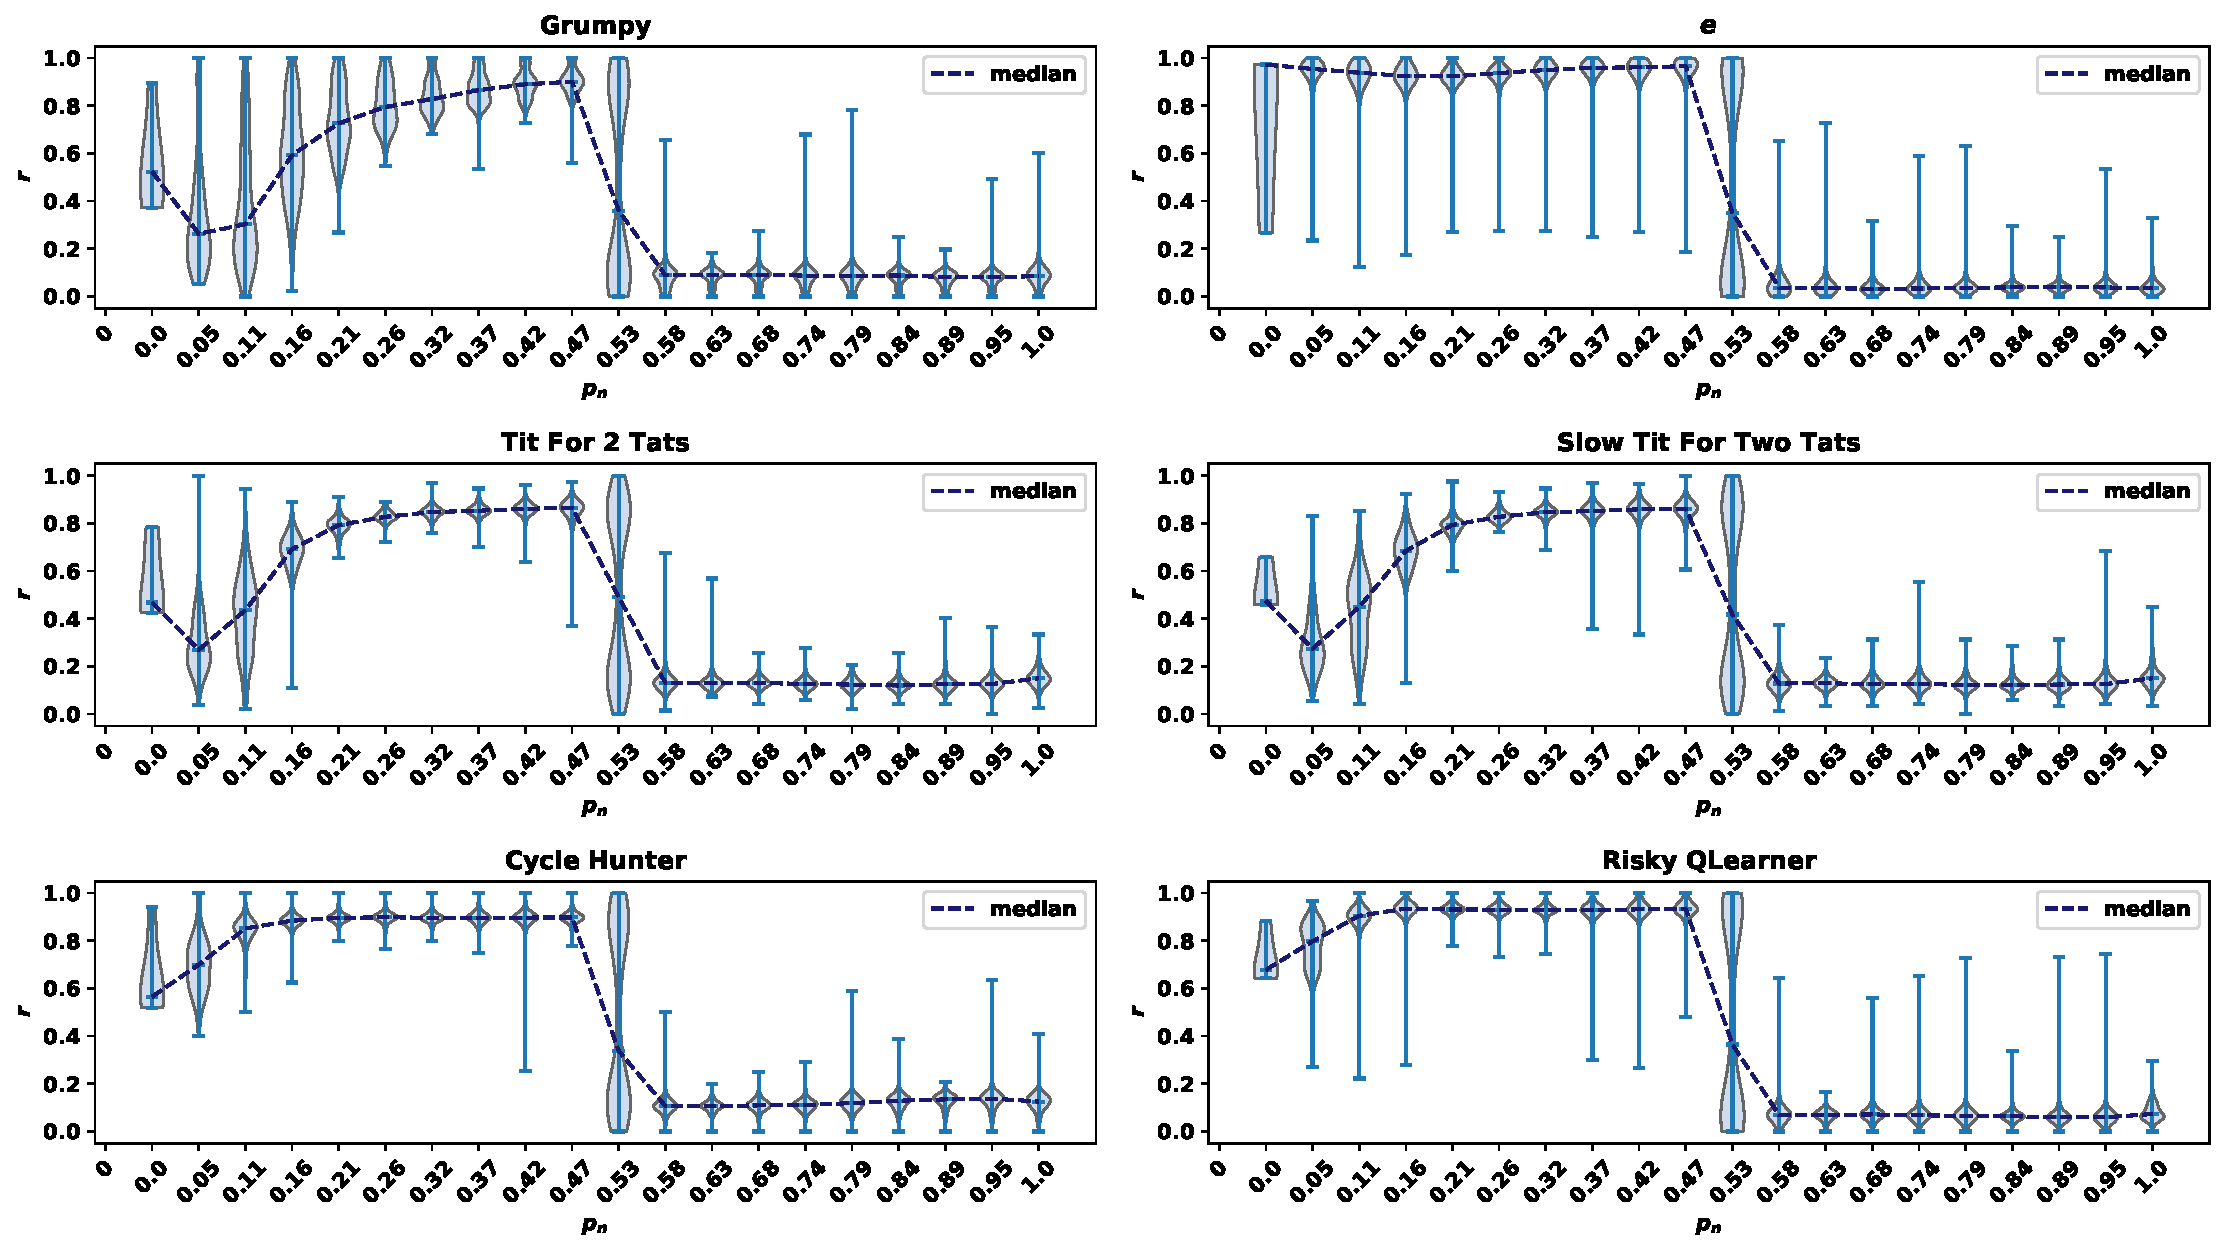
\includegraphics[width=\textwidth]{src/chapters/chapters-04/paper/axlml/images/noise_effect.pdf}
    \caption{\(r\) distributions for top 6 strategies in noisy tournaments over
    the probability of noisy ($p_n$).}
    \label{fig:effect_of_noise}
\end{figure}

\begin{table}[!htbp]
    \centering
    \resizebox{.30\textwidth}{!}{
    \begin{tabular}{lc}
\toprule
Name                      &  $\bar{r}$ \\
\midrule
MEM2                      &    0.06135 \\
Spiteful Tit For Tat      &    0.06344 \\
Nice Meta Winner          &    0.06620 \\
Grudger                   &    0.06667 \\
Meta Winner Long Memory   &    0.07339 \\
Forgiver                  &    0.07362 \\
Fool Me Once              &    0.07362 \\
Meta Winner               &    0.07487 \\
Meta Winner Memory One    &    0.07621 \\
Meta Winner Finite Memory &    0.07692 \\
Meta Winner Deterministic &    0.07792 \\
NMWE Deterministic        &    0.08696 \\
NMWE Long Memory          &    0.08696 \\
CollectiveStrategy        &    0.08696 \\
Defector                  &    0.08889 \\
\bottomrule
\end{tabular}
}
    \caption{Top performances in 5661 noisy tournaments where \(p_n<0.5\).}\label{table:subset_noise_result}
\end{table}

The 15 top ranked strategies in probabilistic ending tournaments include
Fortress 3, Fortress 4 (both introduced in~\cite{Ashlock2006}),
Raider~\cite{Ashlock2014} and Solution B1~\cite{Ashlock2014}, which are
strategies based on finite state automata introduced by Daniel and Wendy
Ashlock. These strategies have been evolved using reinforcement learning, however,
there were trained to maximise their payoffs in tournaments with fixed turns
(150 specifically) and not in probabilistic ending ones. In probabilistic ending
tournaments it appears that the top ranks are mostly occupied by defecting
strategies. These include Better and Better, Gradual Killer, Hard Prober (all
from ~\cite{prison}), Bully (Reverse Tit For Tat)~\cite{Nachbar1992} and
Defector. Thus, it's surprisingly that EasyGo and Fool Me Forever which are
strategies that will defect until their opponent defect, then they will cooperate
until the end, ranked $14^{\text{th}}$ and $15^{\text{th}}$. Upon inspection,
it was found that they are actually the same strategy. This was not known to
the authors at the time of data collection. Figure~\ref{fig:probend_results}
verifies that their performance is the same. Both strategies have repeatedly
ranked highly and there are cases for which they were the winners of the
tournament.

The distributions of the normalised rank in probabilistic ending tournaments,
shown in
Figure~\ref{fig:probend_results}, are less variant than those of noisy
tournaments. The medians of the top 15 strategies are lower than 0.1 and the distributions are skewed
towards 0. Though the large difference between the means and the medians
indicates some outliers, the strategies have overall performed well in the
probabilistic ending tournaments that they participated.

\begin{figure}[h!]
    \centering
    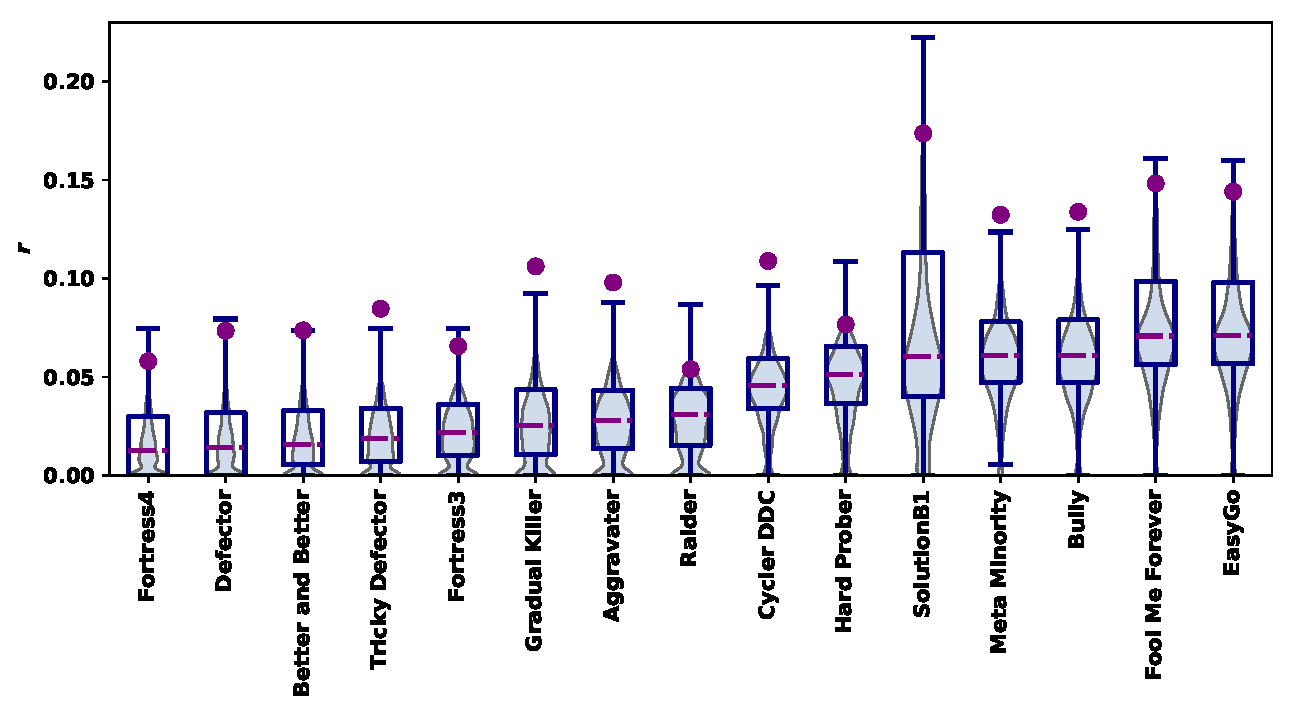
\includegraphics[width=.7\textwidth]{src/chapters/chapters-04/paper/axlml/images/performance_probend.pdf}
    \caption{\(r\) distributions for best performed strategies in probabilistic ending tournaments.}
    \label{fig:probend_results}
\end{figure}

The distributions of \(r\) for the top 6 strategies in probabilistic ending
tournaments over \(p_e\) are given in Figure~\ref{fig:effect_of_probend}.
Figure~\ref{fig:effect_of_probend} shows that the 6 strategies start of with a
high median rank, however, their ranked decreased as the the probability of the
game ending increased and at the point of \(p_e=0.1\) they became the dominant
strategies in their respective tournaments. In essence, what is demonstrated is
that defecting strategies did better when the likelihood of the game ending in
the next turn increased, which is inline with the Folk
Theorem~\cite{Fudenberg2009}. If tournaments where the probability of the game
ending was less than 0.1 were considered then the the top ranked spots are not
dominated by just defecting strategies anymore,
Table~\ref{table:subset_probend_result}. Instead the effective strategies are
now the Meta strategies, trained strategies, Grudger~\cite{axelrodproject} and
Spiteful Tit for Tat~\cite{prison}.

\begin{figure}[!htbp]
    \centering
    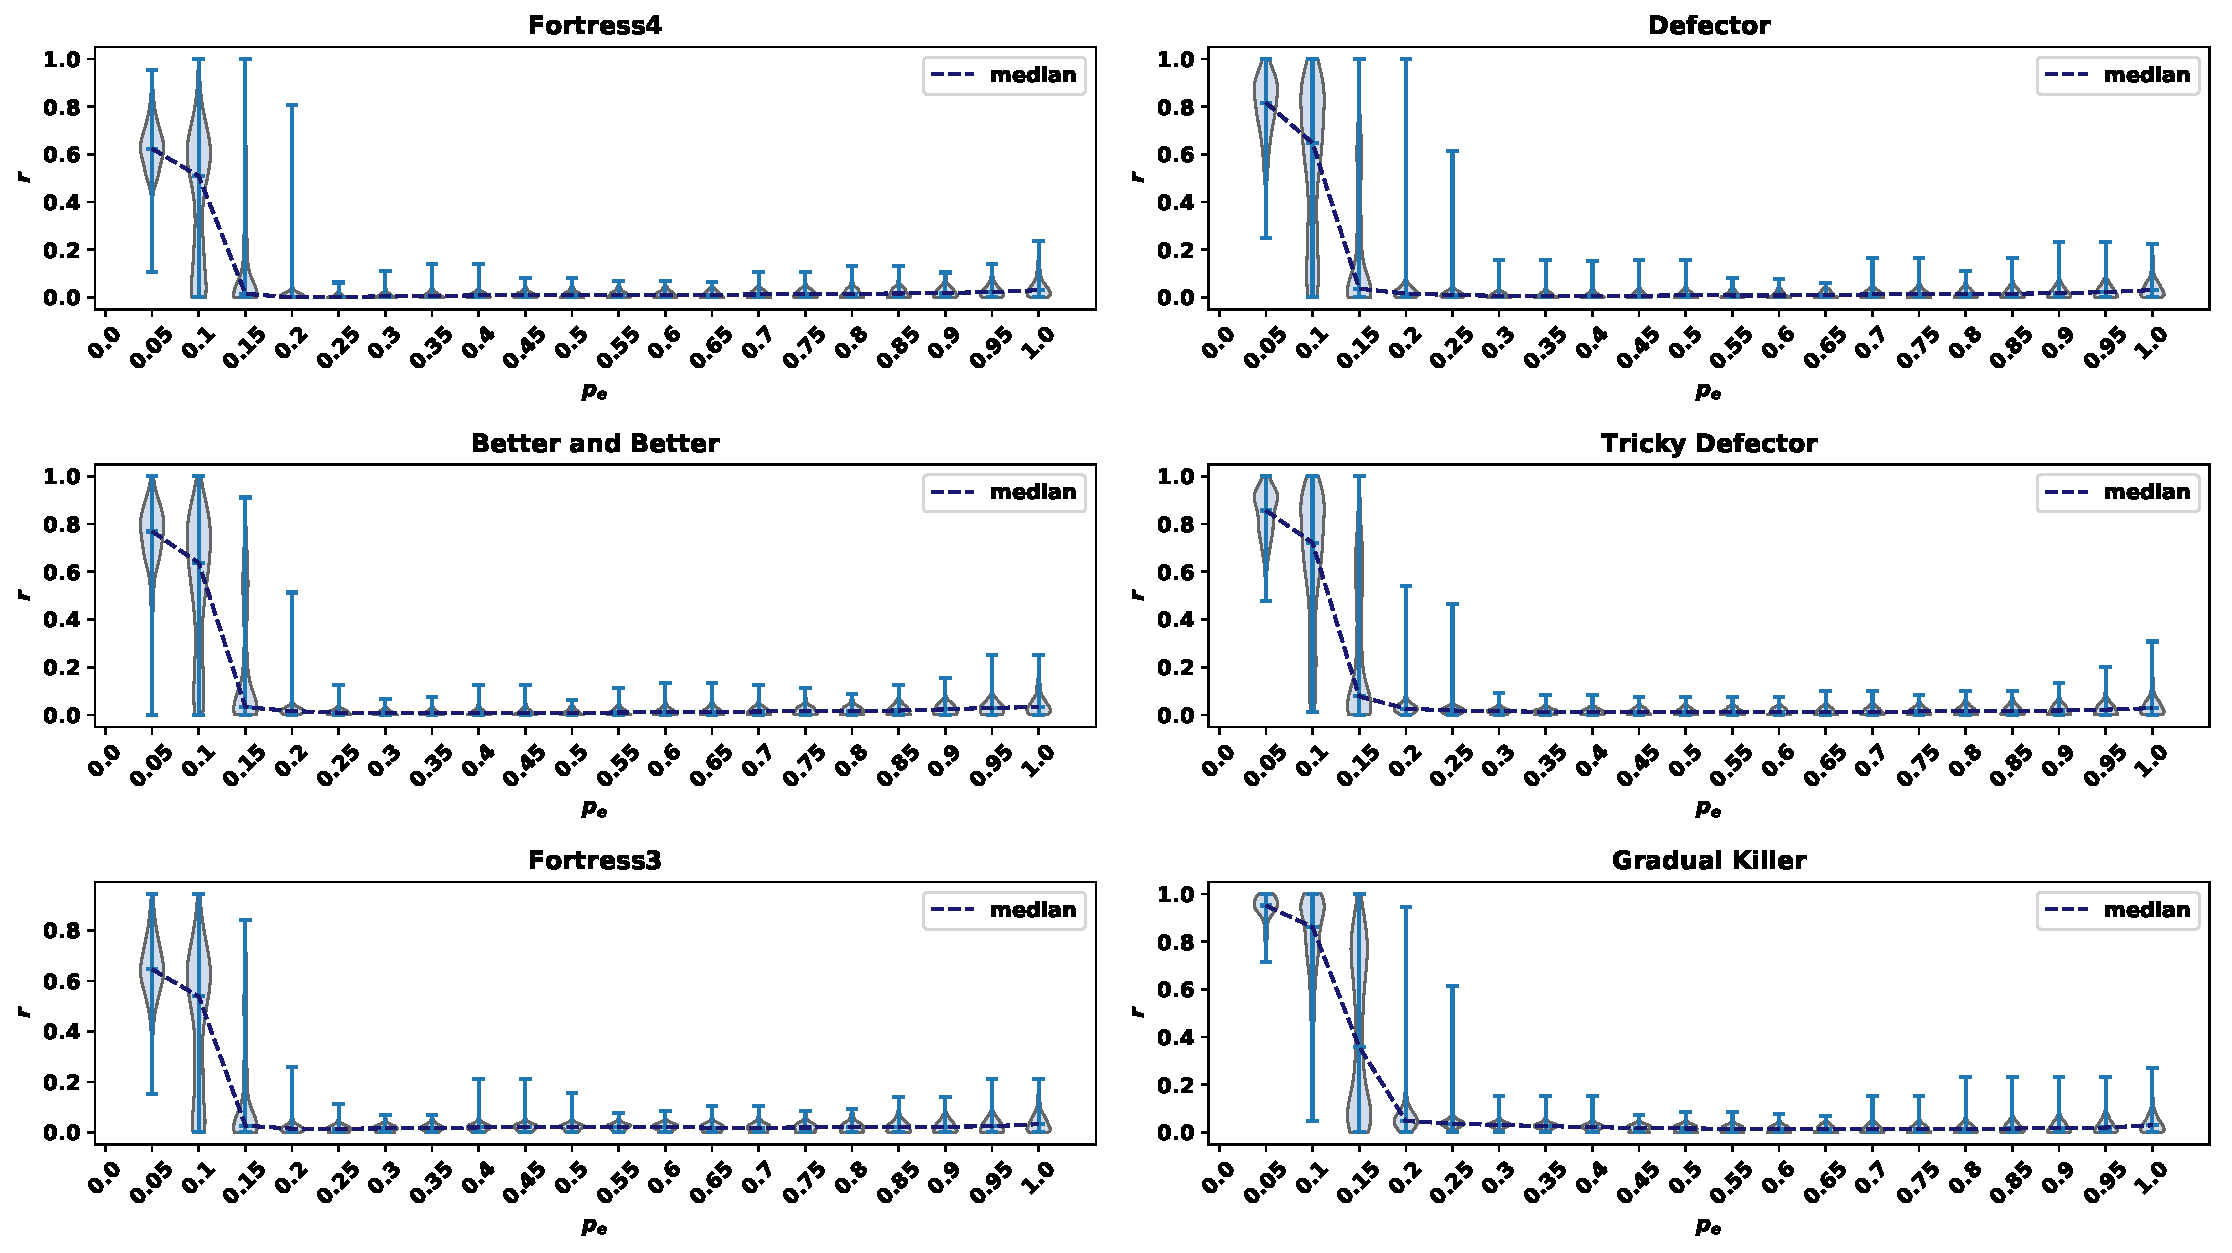
\includegraphics[width=\textwidth]{src/chapters/chapters-04/paper/axlml/images/folk_theorem.pdf}
    \caption{\(r\) distributions for top 6 strategies in probabilistic ending tournaments
    over $p_e$.}
    \label{fig:effect_of_probend}
\end{figure}

\begin{table}[!htbp]
    \centering
    \resizebox{.30\textwidth}{!}{
    \begin{tabular}{lr}
\toprule
Name                      &   $\bar{r}$ \\
\midrule
Evolved FSM 16            &    0.00000 \\
Evolved FSM 16 Noise 05   &    0.01266 \\
MEM2                      &    0.02715 \\
Evolved HMM 5             &    0.04423 \\
EvolvedLookerUp2 2 2      &    0.04870 \\
Spiteful Tit For Tat      &    0.05958 \\
Nice Meta Winner          &    0.06842 \\
NMWE Finite Memory        &    0.06923 \\
Grudger                   &    0.06985 \\
NMWE Deterministic        &    0.07018 \\
NMWE Long Memory          &    0.07407 \\
Nice Meta Winner Ensemble &    0.07595 \\
EvolvedLookerUp1 1 1      &    0.07692 \\
NMWE Memory One           &    0.08000 \\
NMWE Stochastic           &    0.08475 \\
\bottomrule
\end{tabular}
}
    \caption{Top performances in 1139 probabilistic ending tournaments with \(p_e < 0.1\)}
    \label{table:subset_probend_result}
\end{table}

In tournaments with both noise and an unspecified number of turns several of the
top ranked strategies are strategies that were highly ranked in noisy
tournaments. However, strategies from the top ranks in probabilistic ending
tournaments did not rank highly here. Other strategies include $\pi$, $\phi$
which are based on the same approach as $e$. The distributions of \(r\) shown in
Figure~\ref{fig:noisy_probend_results} have the largest median values compared
to the top rank strategies of the other tournament types. A subset of noisy
probabilistic ending tournaments has been considered such that \(p_e < 0.1\) and
\(p_n < 0.5\). The top ranked strategies are given in
Table~\ref{table:subset_probend_noise_result} and it is shown that the Meta
strategies which performed well in noisy tournaments with \(p_n < 0.5\), perform
well once again even the number of turns is not specified. Moreover, several
strategies that did well in probabilistic ending tournaments such as Fortress 3,
Fortress 4, Defector and Better and Better are effective here as well.

\begin{figure}[!htbp]
    \centering
    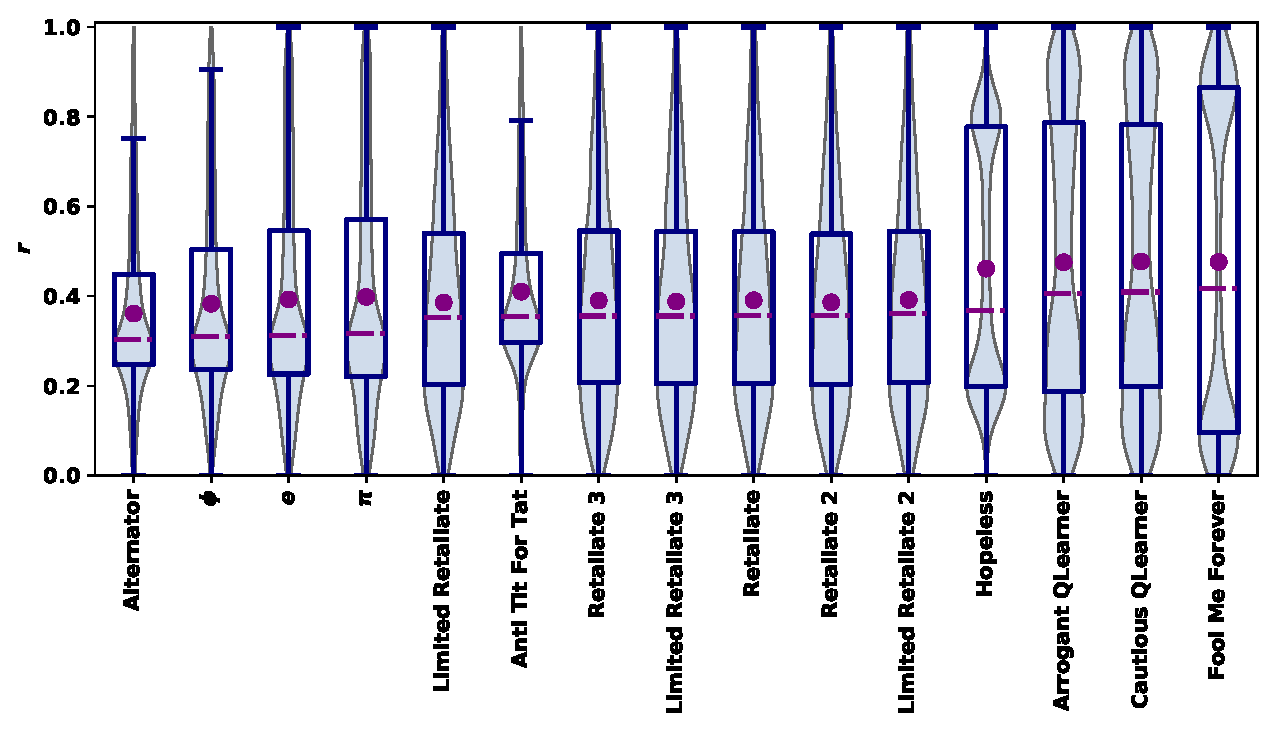
\includegraphics[width=.7\textwidth]{src/chapters/chapters-04/paper/axlml/images/performance_probend_noise.pdf}
    \caption{\(r\) distributions for best performed strategies in noisy
    probabilistic ending tournaments.}
    \label{fig:noisy_probend_results}
\end{figure}

\begin{table}[!htbp]
    \centering
    \resizebox{.30\textwidth}{!}{
    \begin{tabular}{lc}
\toprule
Name                      &    $\bar{r}$\\
\midrule
Defector                  &    0.00552 \\
Better and Better         &    0.01055 \\
Aggravater                &    0.01399 \\
Fortress4                 &    0.02100 \\
Tricky Defector           &    0.03857 \\
Meta Winner Long Memory   &    0.04878 \\
Meta Winner Memory One    &    0.04955 \\
Meta Winner Finite Memory &    0.04972 \\
Meta Winner Stochastic    &    0.05128 \\
Meta Winner Deterministic &    0.05195 \\
Meta Winner               &    0.05333 \\
Meta Winner Ensemble      &    0.05882 \\
Fortress3                 &    0.06956 \\
CollectiveStrategy        &    0.07692 \\
Prober 3                  &    0.08018 \\
\bottomrule
\end{tabular}
}
    \caption{Top performances in 568 probabilistic ending tournaments with \(p_e < 0.1\) and \(p_n < 0.5\).}
    \label{table:subset_probend_noise_result}
\end{table}

Up till now, the performances of the \numberofstrategies strategies have been evaluated for
individual tournament types. The distributions of \(r\) for the tournament types indicate that
for probabilistic ending and standard tournaments successful strategies do exist.
For these settings, the top 15 strategies have frequently ranked in
the top spots with only a few exceptions. Contrarily, it appears that noise
cause variation in the normalised ranks, and the strategies can always guarantee
a spot in the top ranks.

The data set considered in this work, described in
Section~\ref{section:data_collection}, contains a total of \numberofalltournaments
tournament results. For this part of the manuscript the strategies are ranked
based on the median normalised rank they achieved over the entire data set.
The top 15 strategies are given in Table~\ref{table:overall_results}
and their normalised rank distributions are given in Figure~\ref{fig:overall_results}.

\begin{table}[!htbp]
    \centering
    \resizebox{.35\textwidth}{!}{
    \begin{tabular}{lc}
\toprule
Name                       &    $\bar{r}$ \\
\midrule
Limited Retaliate 3        &          0.28609 \\
Retaliate 3                &          0.29630 \\
Retaliate 2                &          0.30250 \\
Limited Retaliate 2        &          0.30328 \\
Limited Retaliate          &          0.31000 \\
Retaliate                  &          0.31707 \\
BackStabber                &          0.32381 \\
DoubleCrosser              &          0.33136 \\
Nice Meta Winner           &          0.34921 \\
PSO Gambler 2 2 2 Noise 05 &          0.35146 \\
Grudger                    &          0.35156 \\
Evolved HMM 5              &          0.35714 \\
NMWE Memory One            &          0.35714 \\
Nice Meta Winner Ensemble  &          0.35870 \\
Forgetful Fool Me Once     &          0.35884 \\
\bottomrule
\end{tabular}
}
    \caption{Top performances over all the tournaments}\label{table:overall_results}
\end{table}

The top ranks include strategies that have been previously mentioned. The
set of Retaliate strategies occupy the top spots followed by BackStabber
and DoubleCrosser. The distributions of the Retaliate strategies have no
statistical difference. Thus, in an IPD tournament where the type is not
specified, playing as any of the Retaliate strategies will have the result.
DoubleCrosser performed well in standard tournaments and the
strategy is just an extension of BackStabber. It should be noted that these
strategies can be characterised as "cheaters". The source code of the strategies
allows them to known the number of turns in a match (if they are specified).
PSO Gambler and Evolved HMM 5 are
trained strategies introduced in~\cite{Harper2017} and Nice Meta Winner and NMWE
Memory One are strategies based on teams. Grudger is a strategy from Axelrod's
original tournament and Forgetful Fool Me Once is based on the same approach as
Grudger. Overall the top 15 strategies are fundamentally different. Some are cheaters,
some are complex, others are simple deterministic strategies and strategies based
on teams. The results of \numberofalltournaments tournaments used in this work imply the following:
they is not a single type of strategy which can performance well in any IPD interaction.

\begin{figure}[!htbp]
    \centering
    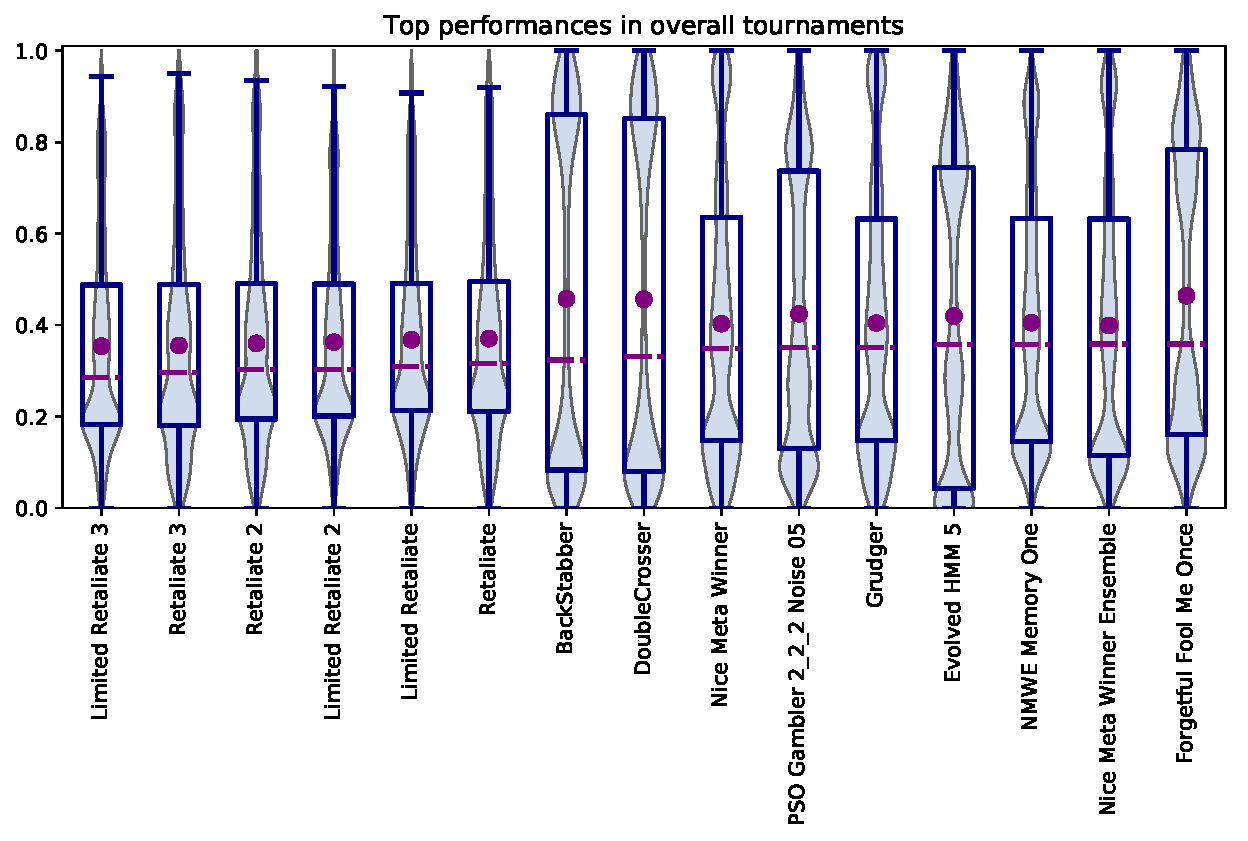
\includegraphics[width=.7\textwidth]{src/chapters/chapters-04/paper/axlml/images/performance_merged.pdf}
    \caption{\(r\) distributions for best performed strategies in the data set~\cite{data}.}
    \label{fig:overall_results}
\end{figure}

This section presented the winning strategies in a series of IPD tournaments. In
standard tournaments the top spots were dominated by complex strategies that had
been trained using reinforcement learning techniques. In noisy environments,
whether the number of turns was fixed or not, the winning strategies were
deterministic strategies designed to defect if the opponent tricked them more
than a current amount of the times that they had tricked their opponent. However,
if a value of noise strictly less than 0.5 was considered, then the successful
strategies were strategies based on teams. In
probabilistic ending tournaments most of the winning strategies were defecting
strategies and trained finite state automata, designed by the same authors.
These strategies only did better when the probability of the game ending after
each turn was increased.
Finally the performance of all \numberofstrategies
strategies over the \numberofalltournaments tournaments in this manuscript was
assessed on \(\bar{r}\). The top ranked strategies were a mixture of behaviours
that did well in standard tournaments and tournaments with noise, as well as a
few strategies based on teams.

The results of this section imply that successful strategies for specific
settings exist for an IPD tournament. The top ranked strategies in both standard
tournaments and tournaments with probabilistic ending, managed to rank in the
top 10\% of the tournament most of the times.
Strategies in noisy
environments demonstrated that no strategy can be consistently
successful, expected if the value of noise is constrained to less than a half.
Overall, there has been not a single strategy that has shown to perform well in
more than one setting. The aim of the next section is to understand which are
the factors that made these strategies successful, in each setting separately
but also overall.

\section{Evaluation of performance}\label{section:evaluation_of_performance}

The aim of this section is to explore the factors that contribute to a
strategy's successful performance. The factors explored are measures regarding a
strategy's behaviour, along with measures regarding the tournaments the
strategies competed in. These are given in Table~\ref{table:manual_measures}.

\newcolumntype{g}{>{\columncolor{Gray}}c}
\begin{table}[h]
    \begin{center}
    \resizebox{\textwidth}{!}{
    \begin{tabular}{gcgcgc}
    \toprule
    measure & measure explanation &  source & value type & min value & max value \\
    \midrule
stochastic  &  If a strategy is stochastic & strategy classifier from~\cite{axelrodproject} & boolean  & Na &  Na \\
makes use of game &  If a strategy makes used of the game information & strategy classifier from~\cite{axelrodproject} & boolean  & Na &  Na \\
makes use of length &  If a strategy makes used of the number of turns & strategy classifier from~\cite{axelrodproject} & boolean  & Na &  Na \\
memory usage &  The memory size of a strategy divided by the number of turns & memory size from~\cite{axelrodproject} & float & 0 &  1 \\
SSE & A measure of how far a strategy is from ZD behaviour & method described in~\cite{Knight2019} & float & 0 & 1 \\
max cooperating rate $(C_{\text{max}})$  & The biggest cooperating rate in a given tournament  & result summary  & float & 0 & 1\\
min cooperating rate $(C_{\text{min}})$ & The smallest cooperating rate in a given tournament  & result summary  & float & 0 & 1\\
median cooperating rate $(C_{\text{median}})$ & The median cooperating rate in a given tournament  & result summary  & float & 0 & 1\\
mean cooperating rate $(C_{\text{mean}})$ & The mean cooperating rate in a given tournament  & result summary  & float & 0 & 1 \\
$C_r$ / $C_{\text{max}}$ & A strategy's cooperating rate divided by the maximum & result summary  & float & 0 & 1 \\
$C_r$ / $C_{\text{min}}$ & A strategy's cooperating rate divided by the minimum & result summary  & float & 0 & 1 \\
$C_r$ / $C_{\text{median}}$ & A strategy's cooperating rate divided by the median  & result summary  & float & 0 & 1\\
$C_r$ / $C_{\text{mean}}$ & A strategy's cooperating rate divided by the mean & result summary  & float & 0 & 1 \\
$C_r$ & The cooperating ratio of a strategy & result summary  & float & 0 & 1 \\
$CC$ to $C$ rate & The probability a strategy will cooperate after a mutual cooperation & result summary  & float & 0 & 1\\
$CD$ to $C$ rate & The probability a strategy will cooperate after being betrayed by the opponent & result summary  & float & 0 & 1 \\
$DC$ to $C$ rate & The probability a strategy will cooperate after betraying the opponent & result summary  & float & 0 & 1 \\
$DD$ to $C$ rate & The probability a strategy will cooperate after a mutual defection & result summary  & float & 0 & 1 \\
$p_n$ & The probability of a player's action being flip at each interaction & trial summary & float & 0 & 1 \\
$n$ & The number of turns & trial summary & integer & 1 & 200 \\
$p_e$ & The probability of a match ending in the next turn & trial summary & float & 0 & 1 \\
$N$ & The number of strategies in the tournament & trial summary & integer & 3 & 195 \\
$k$ & The number of repetitions of a given tournament & trial summary & integer & 10 & 100 \\
    \bottomrule
        \end{tabular}}
    \end{center}
    \caption{The measures which are included in the performance evaluation analysis.}
    \label{table:manual_measures}
\end{table}

Axelrod-Python makes use of classifiers to classify strategies according to
various dimensions. These determine whether
a strategy is stochastic or deterministic, whether it makes use of the number of
turns or the game's payoffs. The memory usage measure is calculated as the
memory size of strategy (which is specified in the strategies implementation
in~\cite{axelrodproject}) divide by the number of turns. For example, Evolved
FSM 16 Noise 05 has a memory size of 16 and participated in a tournament where
$n$ was 134. In the given tournament Evolved FSM 16 Noise 05 has a memory usage
of 0.119. For tournaments with a probabilistic ending the number of turns was
not collected, so the memory usage measure is not used for probabilistic ending
tournaments. The SSE is a measure introduced in~\cite{Knight2019} which shows
how close a strategy is to behaving as a ZDs, and subsequently, in an
extortionate way. The method identifies the ZDs closest to a given strategy and
calculates the algebraic distance between them, defined as SSE. A SSE value of 1
indicates no extortionate behaviour at all whereas a value of 0 indicates that a
strategy is behaving a ZDs. The rest of the factors considered are the $CC$ to
$C$, $CD$ to $C$, $DC$ to $C$, and $DD$ to $C$ rates as well as cooperating
ratio of a strategy. The minimum, maximum, medium and median cooperating ratios
of each tournament are also included, and finally the number of turns, the
number of strategies, the number of repetitions and the probabilities of noise
and the game ending are also included.

Table~\ref{table:correlations} shows the correlation coefficients between the
measures of Table~\ref{table:manual_measures} the median score and the median
normalised rank. Note that the correlation for the classifiers is
not included because they are binary variables and they will be evaluated using a
different method. The correlation coefficients for all the measures in
Table~\ref{table:manual_measures} against themselves have also been calculated and a
graphical representation can be found in the Appendix~\ref{app:correlations}.

\newcolumntype{g}{>{\columncolor{Gray}}c}
\begin{table}[!htbp]
    \begin{center}
    \resizebox{.9\textwidth}{!}{
        \begin{tabular}{lggccggccggg}
    \toprule
    &  \multicolumn{2}{g}{Standard} & \multicolumn{2}{c}{Noisy} & \multicolumn{2}{g}{Probabilistic ending} &  \multicolumn{2}{c}{Noisy probabilistic ending} &  \multicolumn{2}{g}{Overall} \\
\midrule
{} &  $r$ &  median score &  $r$ &  median score &  $r$ &  median score &  $r$ &  median score &  $r$ &  median score\\
\midrule
$CC$ to $C$ rate     & -0.501 &  0.501 &   0.414 &  -0.504 &   0.408 &  -0.323 &   0.260 &   0.022 &  -0.501 &  0.501 \\
$CD$ to $C$ rate     &  0.226 & -0.199 &   0.456 &  -0.330 &   0.320 &  -0.017 &   0.205 &  -0.220 &   0.226 & -0.199 \\
$C_r$                & -0.323 &  0.384 &   0.711 &  -0.678 &   0.714 &  -0.832 &   0.579 &  -0.135 &  -0.323 &  0.384 \\
$C_r$ / $C_{max}$    & -0.323 &  0.381 &   0.616 &  -0.551 &   0.714 &  -0.833 &   0.536 &  -0.116 &  -0.323 &  0.381 \\
$C_r$ / $C_{mean}$   & -0.331 &  0.358 &   0.731 &  -0.740 &   0.721 &  -0.861 &   0.649 &  -0.621 &  -0.331 &  0.358 \\
$C_r$ / $C_{median}$ & -0.331 &  0.353 &   0.652 &  -0.669 &   0.712 &  -0.852 &   0.330 &  -0.466 &  -0.331 &  0.353 \\
$C_r$ / $C_{min}$    &  0.109 & -0.080 &  -0.358 &   0.250 &  -0.134 &   0.150 &  -0.368 &   0.113 &   0.109 & -0.080 \\
$C_{max}$            & -0.000 &  0.049 &   0.000 &   0.023 &  -0.000 &   0.046 &   0.000 &  -0.004 &  -0.000 &  0.049 \\
$C_{mean}$           & -0.000 &  0.229 &  -0.000 &   0.271 &   0.000 &   0.200 &   0.000 &   0.690 &  -0.000 &  0.229 \\
$C_{median}$         &  0.000 &  0.209 &  -0.000 &   0.240 &  -0.000 &   0.187 &  -0.000 &   0.673 &   0.000 &  0.209 \\
$C_{min}$            &  0.000 &  0.084 &   0.000 &  -0.017 &  -0.000 &   0.007 &  -0.000 &   0.041 &   0.000 &  0.084 \\
$DC$ to $C$ rate     &  0.127 & -0.100 &   0.509 &  -0.504 &  -0.018 &   0.033 &   0.341 &  -0.016 &   0.127 & -0.100 \\
$DD$ to $C$ rate     &  0.412 & -0.396 &   0.533 &  -0.436 &  -0.103 &   0.176 &   0.378 &  -0.263 &   0.412 & -0.396 \\
$N$                  &  0.000 & -0.009 &  -0.000 &   0.002 &  -0.000 &   0.003 &  -0.000 &   0.001 &   0.000 & -0.009 \\
$k$                  &  0.000 & -0.002 &  -0.000 &   0.003 &  -0.000 &   0.001 &  -0.000 &  -0.008 &   0.000 & -0.002 \\
$n$                  &  0.000 & -0.125 &  -0.000 &  -0.024 &       - &       - &       - &       - &   0.000 & -0.125 \\
$p_e$                &      - &      - &        - &     - &    0.000 &   0.165 &   0.000 &  -0.058 &  -0.001 &  0.001 \\
$p_n$                &      - &      - &  -0.000 &   0.207 &       - &       - &  -0.000 &  -0.650 &   0.002 & -0.000 \\
Make use of game     & -0.003 & -0.022 &   0.025 &  -0.082 &  -0.053 &  -0.108 &   0.013 &  -0.016 &  -0.003 & -0.022 \\
Make use of length   & -0.158 &  0.124 &   0.005 &  -0.123 &  -0.025 &  -0.090 &   0.014 &  -0.016 &  -0.154 &  0.117 \\
SSE                  &  0.473 & -0.452 &   0.463 &  -0.337 &  -0.156 &   0.223 &   0.305 &  -0.259 &   0.473 & -0.452 \\
memory usage         & -0.082 &  0.095 &  -0.007 &  -0.017 &       - &     - &     - &           - &  -0.084 &  0.095 \\
stochastic           &  0.006 & -0.024 &   0.022 &  -0.026 &   0.002 &  -0.130 &   0.021 &  -0.013 &   0.006 & -0.024 \\
\bottomrule
\end{tabular}

    }
\end{center}
\caption{Correlations table between the measures of Table~\ref{table:manual_measures}
the normalised rank and the median score.}\label{table:correlations}
\end{table}

In standard tournaments the measures  $CC$ to $C$, $C_r$, $C_r / C_{\text{max}}$
and the cooperating ratio compared to $C_{\text{median}}$ and $C_{\text{mean}}$
have a moderate negative effect on the normalised rank, and a moderate positive
on the median score. The SSE error and the $DD$ to $C$ have the opposite
effects. Thus, in standard tournaments behaving cooperatively corresponds to a
more successful performance. Even though being nice pays off,
that's not true against defective strategies. Cooperating after a mutual
defection lowers a strategy's success.
Figure~\ref{fig:rates_of_winners_in_standard_tournaments} confirms that the
winners of standard tournaments always cooperate after a mutual cooperation and
almost always defects after a mutual defection.

\begin{figure}[!htbp]
    \centering
    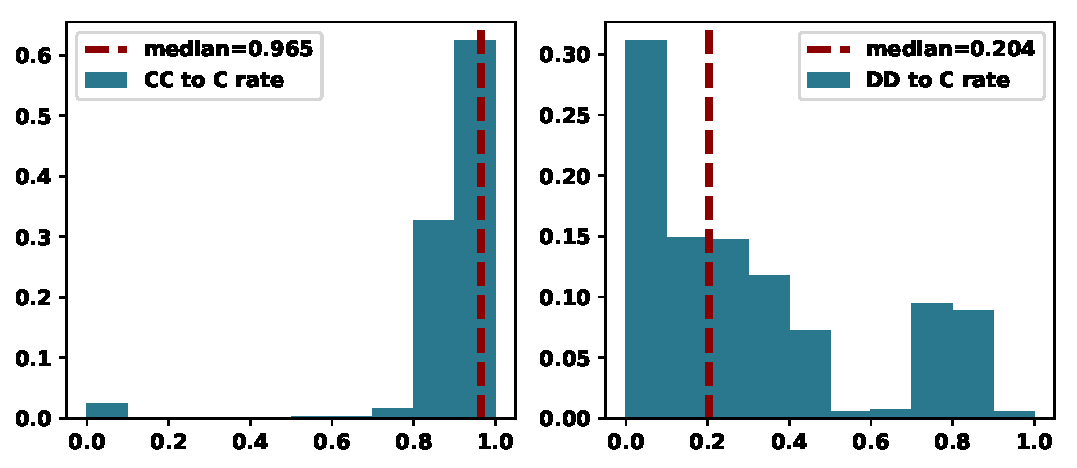
\includegraphics[width=.65\textwidth]{src/chapters/chapters-04/paper/axlml/images/rates_of_winners_in_standard_tournaments.pdf}
    \caption{Distributions of $CC$ to $C$ and $DD$ to $C$ for the winners in
    standard tournaments.}\label{fig:rates_of_winners_in_standard_tournaments}
\end{figure}

Compared to standard tournaments, in both noisy and in probabilistic ending
tournaments the higher the rates of cooperation the lower a strategy's success
and median score. A strategy would want to cooperate less than both
the mean and median cooperator in such settings. In probabilistic ending
tournaments the correlations coefficients have a larger values, indicating a
stronger effect. Thus a strategy will be punished more by it's cooperative
behaviour in probabilistic ending environments, this was seen in Section~\ref{section:evaluation_of_performance}
as well. The distributions of the $C_r$ of the winners in
both tournaments is given by Figure~\ref{fig:c_r_distributions}. It confirms
that the winners in noisy tournaments cooperated less than 35\% of the times
and in probabilistic ending tournaments less than 10\%.
In noisy probabilistic ending tournaments and in over all the tournaments' results,
the only measures that had a moderate affect are $C_r/C_{\text{mean}},
C_r/C_{\text{max}}$ and $C_r$. In such environments cooperative behaviour
appears to be punished by not as much as in noisy and probabilistic ending
tournaments.

\begin{figure}[!htbp]
    \centering
    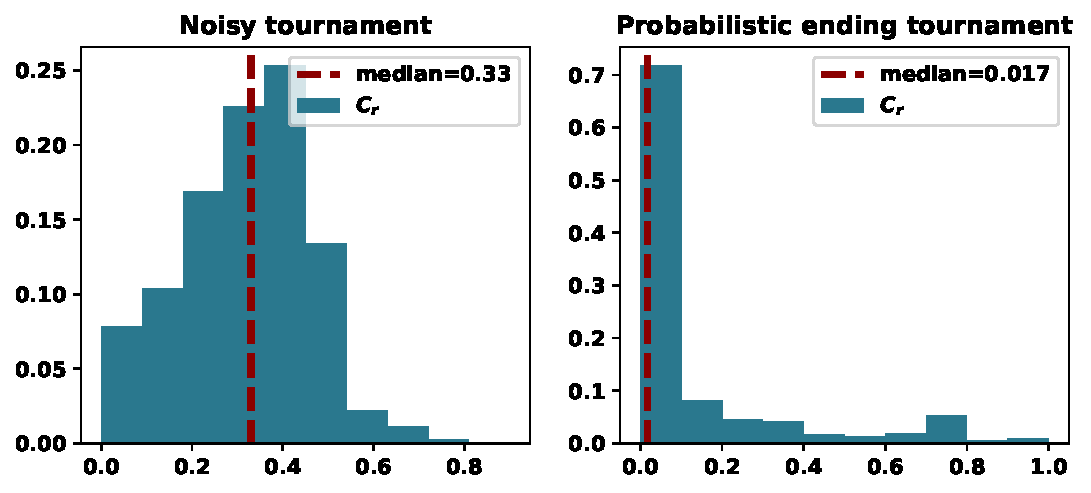
\includegraphics[width=.65\textwidth]{src/chapters/chapters-04/paper/axlml/images/c_r_winners_tournaments.pdf}
    \caption{$C_r$ distributions of the winners in noisy and in probabilistic
    ending tournaments.}\label{fig:c_r_distributions}
\end{figure}

The performances are clustered based on the normalised rank. More specifically,
they are clustered 3 times into 2 different clusters based on  on whether their
normalised rank was in the top 5\%, 25\% or 50\% respectively. A random forest
approach~\cite{breiman2001} is then applied to each performance to predict the cluster to
which it has been assigned to. The random forest method
constructs many individual decision trees and the predictions from all trees are
pooled to make the final prediction. The random forest models are trained on a
training set of 70\% of the tournaments results. The accuracy of each model
based on $R^2$ are given by Table~\ref{table:accuracy_random_forest}. The out of
the bag error~\cite{hastie2005} has also been calculated. The models fit well,
and a high value of both the accuracy measure on the test data and the OOB error
indicate that the model is not over fitting.

The performances have also been clustered based on their normalised rank and
their median score by a \(k-\)means algorithm~\cite{Arthur2007}. The number of
clusters is not deterministically chosen but it is based on the silhouette
coefficients~\cite{Rousseeuw1987}. The chosen cluster for each tournament type,
as well as the accuracy for random forest models are also given in
Table~\ref{table:accuracy_random_forest}.

\begin{table}[!htbp]
    \begin{center}
        \resizebox{.9\textwidth}{!}{
        \begin{tabular}{lccccc}
    \toprule
    Tournament type & Clustering on & Number of clusters & $R^2$ training data &  $R^2$ test data  & $R^2$ OOB score\\
    \midrule
    standard  & top 5\% $r$              & 2  & 0.998831  & 0.987041 & 0.983708 \\
              & top 25\% $r$             & 2  & 0.998643  & 0.978626 & 0.969202 \\
              & top 50\% $r$             & 2  & 0.998417  & 0.985217 & 0.976538 \\
              & $r$  \& normalised score & 2  & 0.998794  & 0.990677 & 0.982959 \\
    \midrule
    noisy     & top 5\% $r$              & 2 & 0.996677  & 0.950572 & 0.935383\\
              & top 25\% $r$             & 2 & 0.996677  & 0.950572 & 0.935383\\
              & top 50\% $r$             & 2 & 0.996677  & 0.950572 & 0.935383\\
              & $r$  \& normalised score & 3 & 0.996677  & 0.950572 & 0.935383\\
    \midrule
    probabilistic ending & top 5\% $r$              & 2 & 0.999592  & 0.995128 & 0.992819 \\
                         & top 25\% $r$             & 2 & 0.999592  & 0.995128 & 0.992819 \\
                         & top 50\% $r$             & 2 & 0.999592  & 0.995128 & 0.992819 \\
                         & $r$  \& normalised score & 2 & 0.999592  & 0.995128 & 0.992819 \\
    \midrule
    noisy probabilistic ending & top 5\% $r$              & 2 & 0.990490  & 0.813905 & 0.791418\\
                               & top 25\% $r$             & 2 & 0.990490  & 0.813905 & 0.791418\\
                               & top 50\% $r$             & 2 & 0.990490  & 0.813905 & 0.791418\\
                               & $r$  \& normalised score & 4 & 0.990490  & 0.813905 & 0.791418\\
    \midrule
    over \numberofalltournaments tournaments & top 5\% $r$               & 2 & 0.993396 & 0.913409 & 0.898059 \\
                                             & top 25\% $r$              & 2 & 0.993396 & 0.913409 & 0.898059 \\
                                             & top 50\% $r$              & 2 & 0.993396 & 0.913409 & 0.898059 \\
                                             & $r$  \& normalised score  & 3 & 0.993396 & 0.913409 & 0.898059 \\
    \bottomrule
        \end{tabular}}
    \end{center}
    \caption{Accuracy metrics for random forest models.}
    \label{table:accuracy_random_forest}
\end{table}

The importance that the measures of Table~\ref{table:manual_measures} had on
each classification task; to which cluster a performance was assigned to based
on the normalised rank, and their normalised rank and median score have been
calculated and are given by Figures~\ref{fig:clustering_importance_standard},
\ref{fig:clustering_importance_noise},~\ref{fig:clustering_importance_probend},
\ref{fig:clustering_importance_probend_noise}
and~\ref{fig:clustering_importance_overall}. These show that the classifiers
stochastic, make use of game and make use of length have no significant effect,
and several of the measures that are highted by the importance are inline with
the correlation results. Moreover, the smoothing parameter \(k\) appears to no
have a significant effect either. The most important measures based on the
random forest analysis were $C_{r} / C_{median}$ and $C_r / C_{mean}$.

\begin{figure}[!htbp]
    \begin{subfigure}[t]{0.5\textwidth}
        \begin{center}
            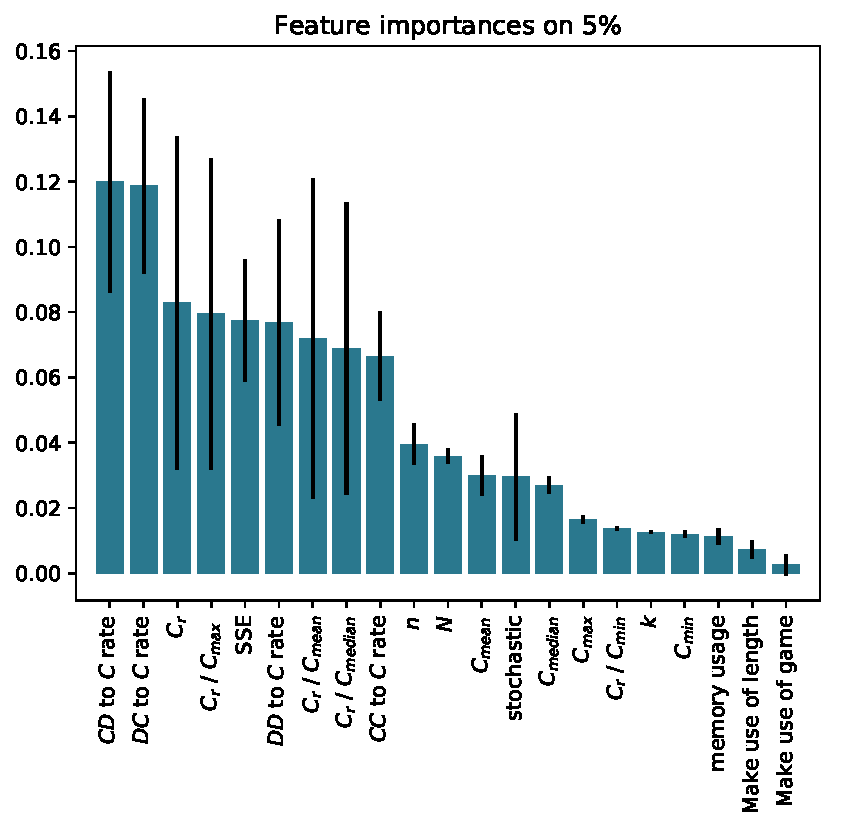
\includegraphics[width=.75\linewidth]{src/chapters/chapters-04/paper/axlml/new_output/standard/_feature_importance_bar_plot_cluster_on_0_05.pdf}
        \end{center}
        \caption{Importance of features for clusters on 5\% performance.}
    \end{subfigure}\hfill
    \begin{subfigure}[t]{0.5\textwidth}
        \begin{center}
            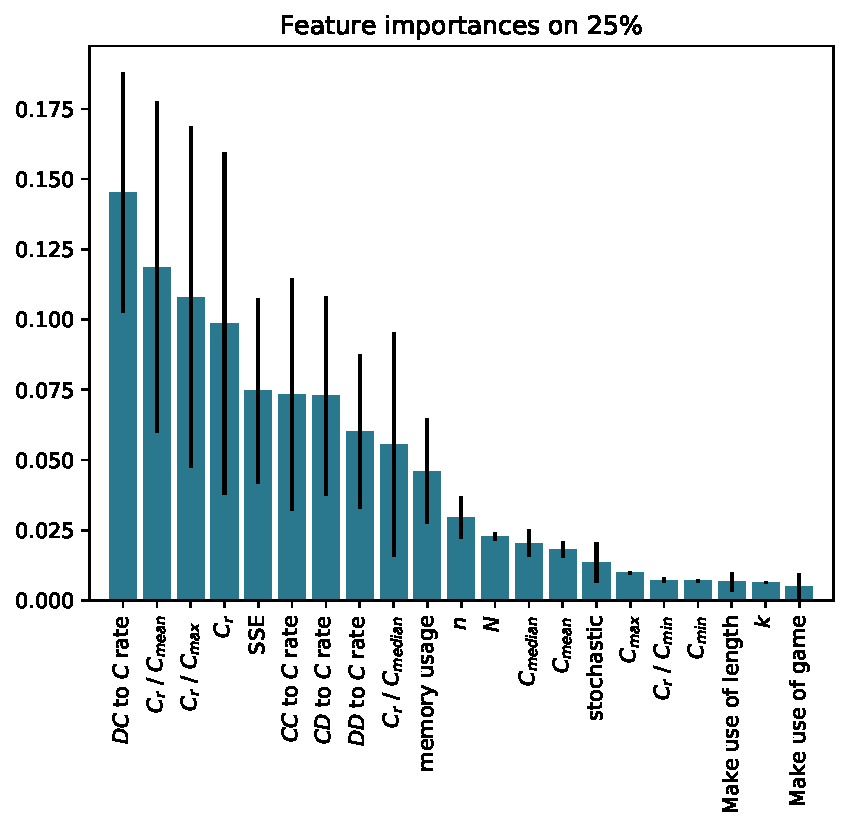
\includegraphics[width=.75\linewidth]{src/chapters/chapters-04/paper/axlml/new_output/standard/_feature_importance_bar_plot_cluster_on_0_25.pdf}
        \end{center}
        \caption{Importance of features for clusters on 25\% performance.}
    \end{subfigure}
    \begin{subfigure}[t]{0.5\textwidth}
        \begin{center}
            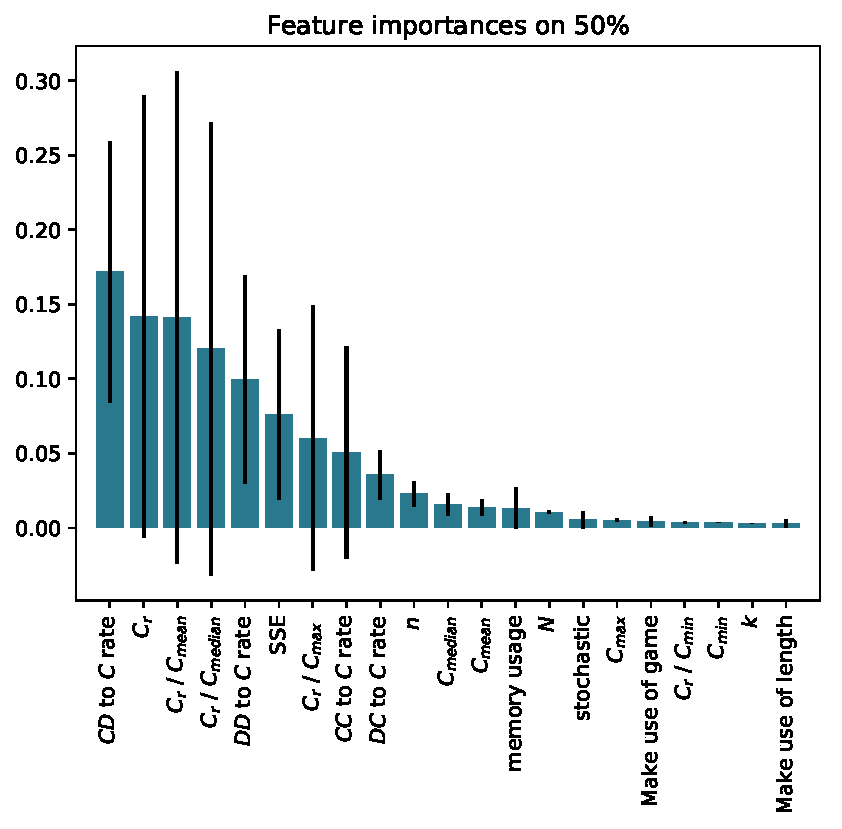
\includegraphics[width=.75\linewidth]{src/chapters/chapters-04/paper/axlml/new_output/standard/_feature_importance_bar_plot_cluster_on_0_5.pdf}
        \end{center}
        \caption{Importance of features for clusters on 50\% performance.}
    \end{subfigure}\hfill
    \begin{subfigure}[t]{0.5\textwidth}
        \begin{center}
            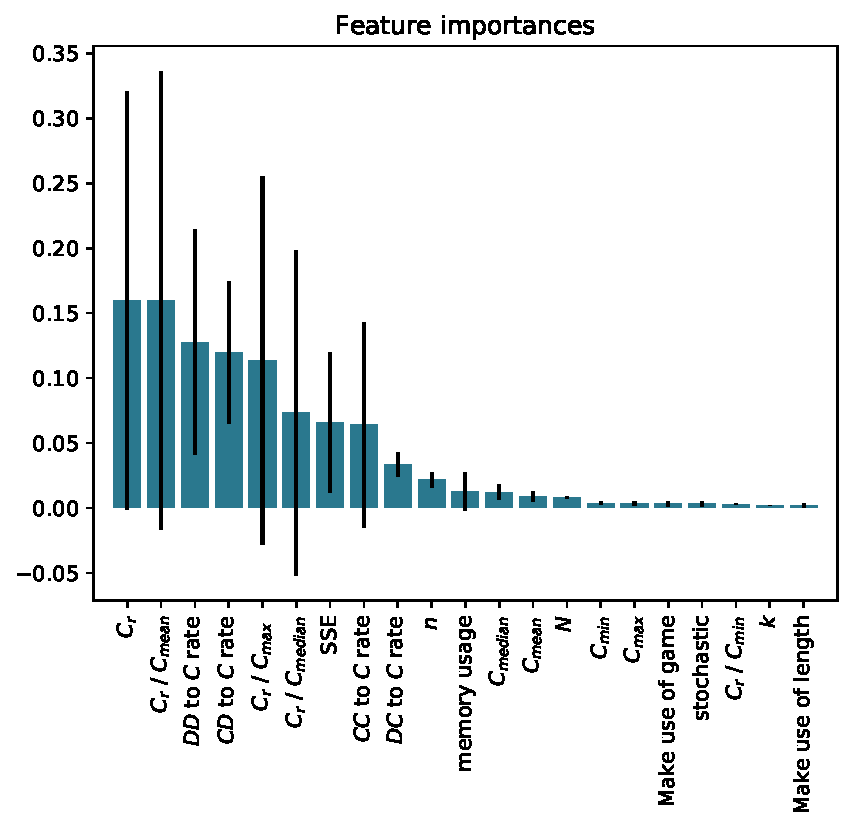
\includegraphics[width=.75\linewidth]{src/chapters/chapters-04/paper/axlml/k_means_output/standard/_feature_importance_bar_plot.pdf}
        \end{center}
        \caption{Importance of features for clusters based on \(k\)means algorithm.}
    \end{subfigure}
    \caption{Importance of features in standard tournaments for different
    clustering methods.}\label{fig:clustering_importance_standard}
\end{figure}

\begin{figure}[!htbp]
    \begin{subfigure}{0.5\textwidth}
        \begin{center}
            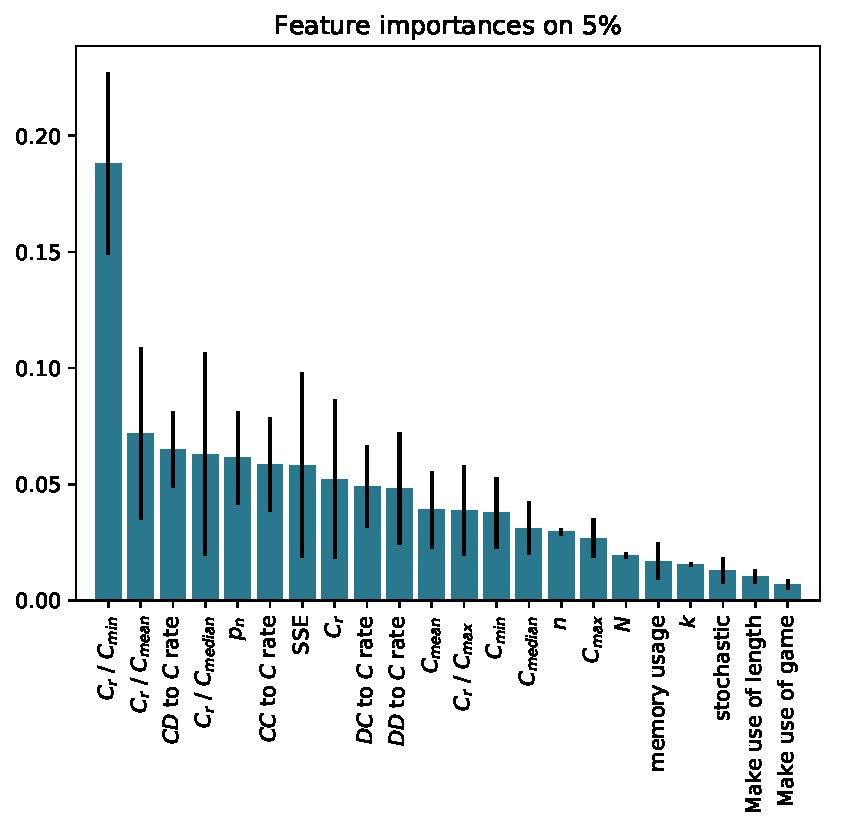
\includegraphics[width=.75\linewidth]{src/chapters/chapters-04/paper/axlml/new_output/noise/_feature_importance_bar_plot_cluster_on_0_05.pdf}
        \end{center}
        \caption{Importance of features for clusters on 5\% performance.}
    \end{subfigure}\hfill
    \begin{subfigure}{0.5\textwidth}
        \begin{center}
            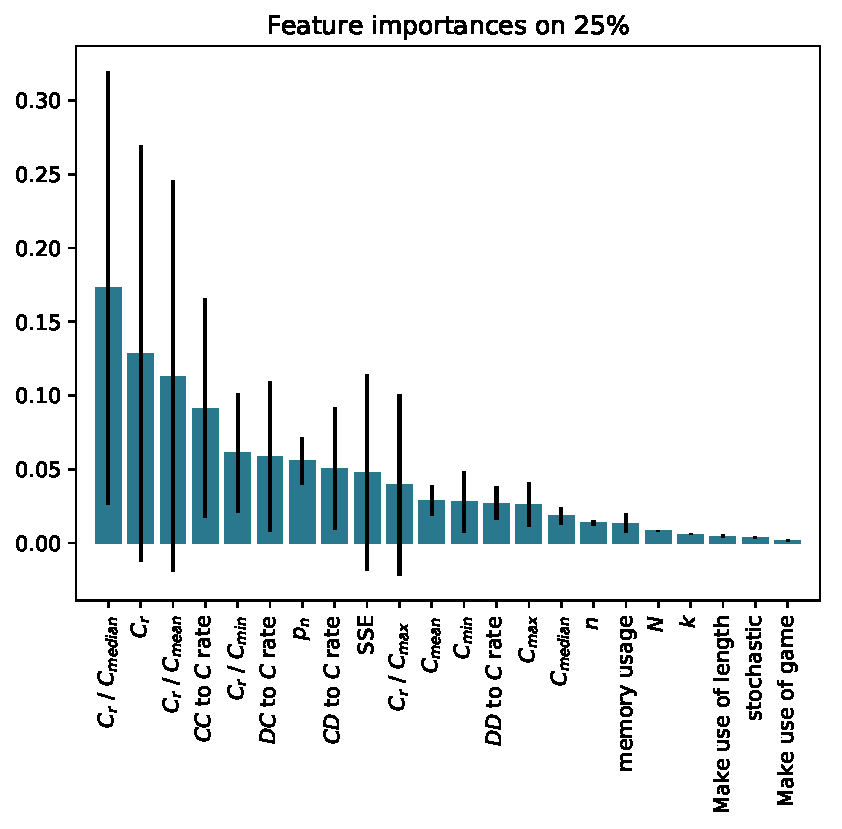
\includegraphics[width=.75\linewidth]{src/chapters/chapters-04/paper/axlml/new_output/noise/_feature_importance_bar_plot_cluster_on_0_25.pdf}
        \end{center}
        \caption{Importance of features for clusters on 25\% performance.}
    \end{subfigure}
    \begin{subfigure}{0.5\textwidth}
        \begin{center}
            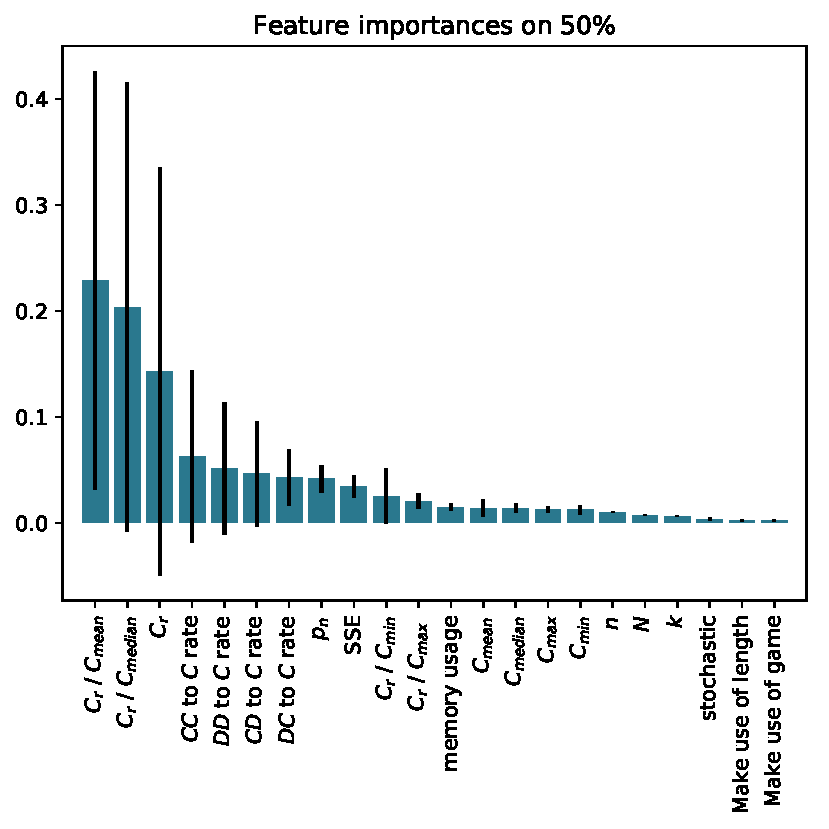
\includegraphics[width=.75\linewidth]{src/chapters/chapters-04/paper/axlml/new_output/noise/_feature_importance_bar_plot_cluster_on_0_5.pdf}
        \end{center}
        \caption{Importance of features for clusters on 50\% performance.}
    \end{subfigure}\hfill
    \begin{subfigure}{0.5\textwidth}
        \begin{center}
            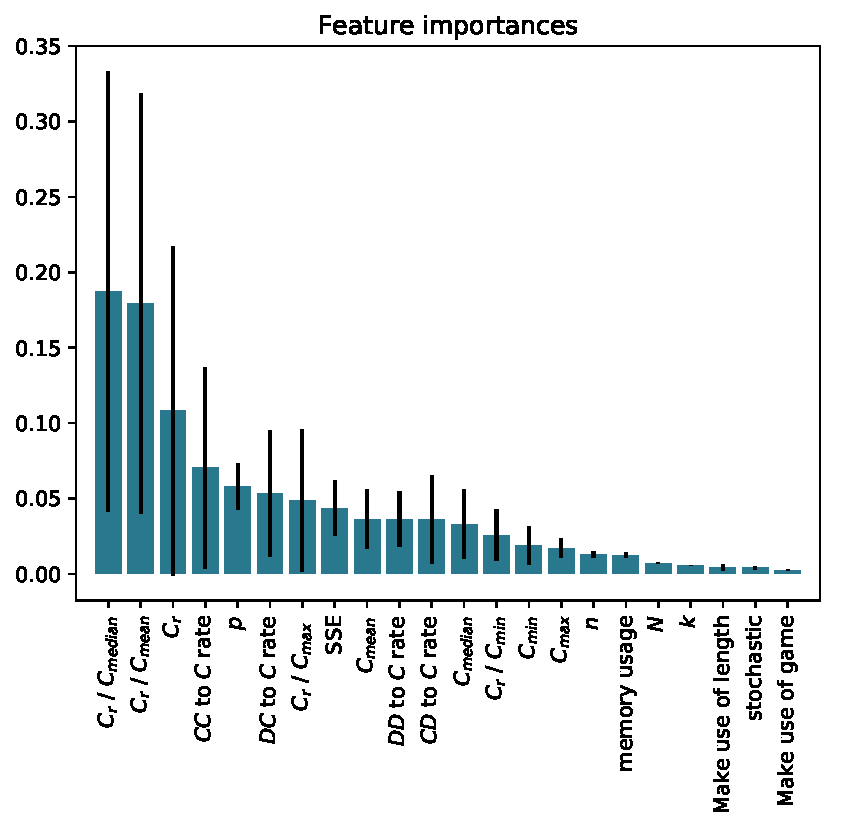
\includegraphics[width=.75\linewidth]{src/chapters/chapters-04/paper/axlml/k_means_output/noise/_feature_importance_bar_plot.pdf}
        \end{center}
        \caption{Importance of features for clusters based on \(k\)means algorithm.}
    \end{subfigure}
    \caption{Importance of features in noisy tournaments for different
    clustering methods.}\label{fig:clustering_importance_noise}
\end{figure}

\begin{figure}[!htbp]
    \begin{subfigure}[t]{0.5\textwidth}
        \begin{center}
            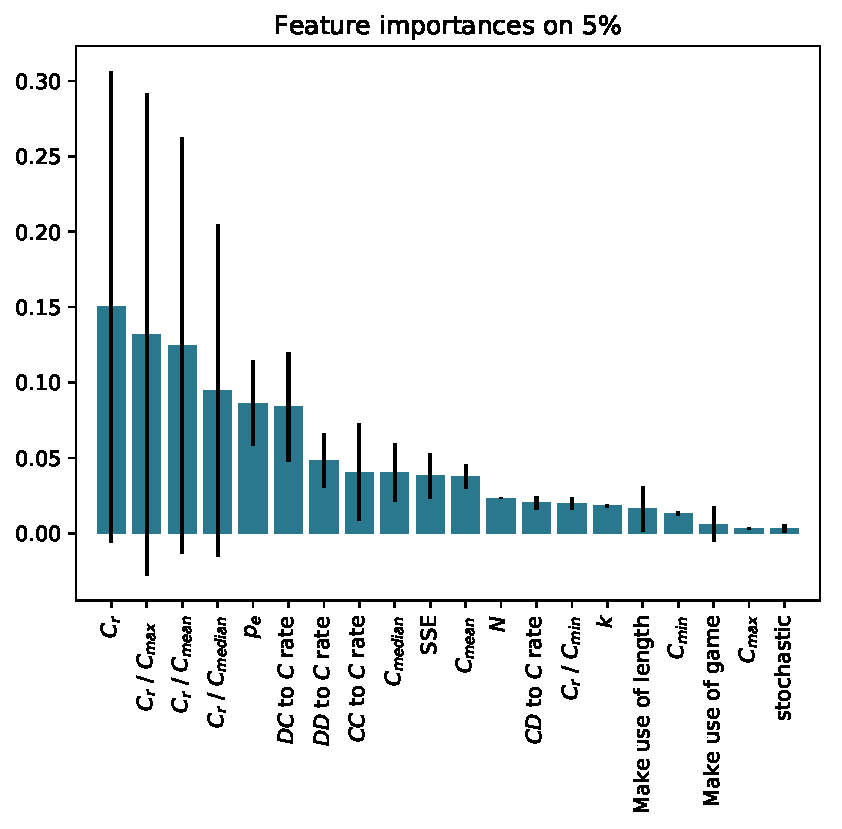
\includegraphics[width=.75\linewidth]{src/chapters/chapters-04/paper/axlml/new_output/probend/_feature_importance_bar_plot_cluster_on_0_05.pdf}
        \end{center}
        \caption{Importance of features for clusters on 5\% performance.}
    \end{subfigure}
    \begin{subfigure}[t]{0.5\textwidth}
        \begin{center}
            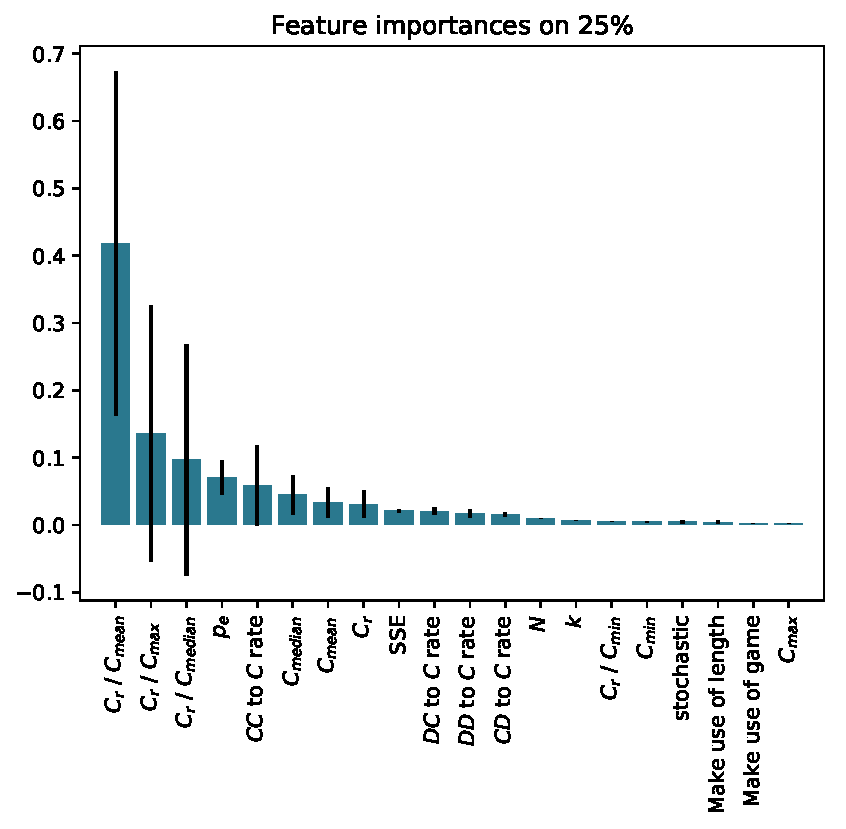
\includegraphics[width=.75\linewidth]{src/chapters/chapters-04/paper/axlml/new_output/probend/_feature_importance_bar_plot_cluster_on_0_25.pdf}
        \end{center}
        \caption{Importance of features for clusters on 25\% performance.}
    \end{subfigure}
    \begin{subfigure}[t]{0.5\textwidth}
        \begin{center}
            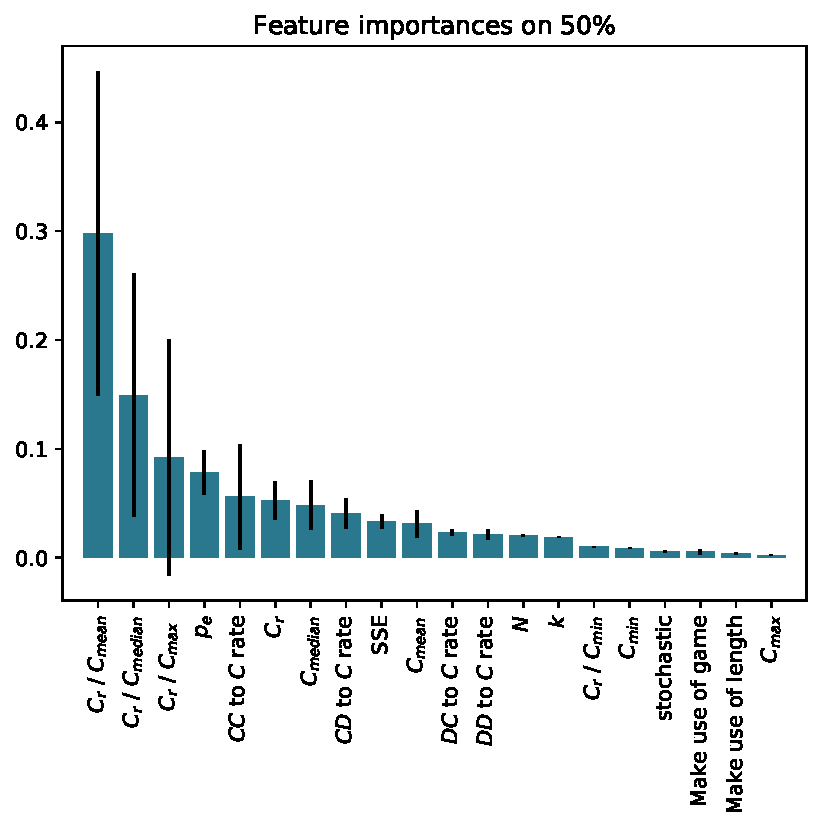
\includegraphics[width=.75\linewidth]{src/chapters/chapters-04/paper/axlml/new_output/probend/_feature_importance_bar_plot_cluster_on_0_5.pdf}
        \end{center}
        \caption{Importance of features for clusters on 50\% performance.}
    \end{subfigure}
    \begin{subfigure}[t]{0.5\textwidth}
        \begin{center}
            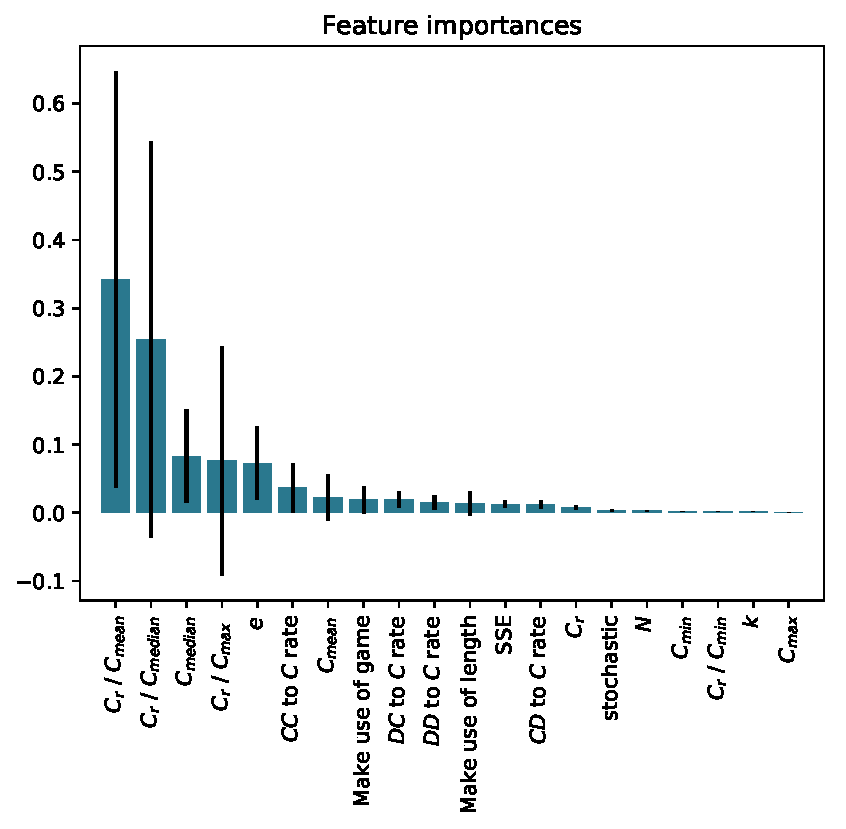
\includegraphics[width=.75\linewidth]{src/chapters/chapters-04/paper/axlml/k_means_output/probend/_feature_importance_bar_plot.pdf}
        \end{center}
        \caption{Importance of features for clusters based on \(k\)means algorithm.}
    \end{subfigure}
    \caption{Importance of features in probabilistic ending tournaments for different
    clustering methods.}\label{fig:clustering_importance_probend}
\end{figure}

\begin{figure}[!htbp]
    \begin{subfigure}[t]{0.5\textwidth}
        \begin{center}
            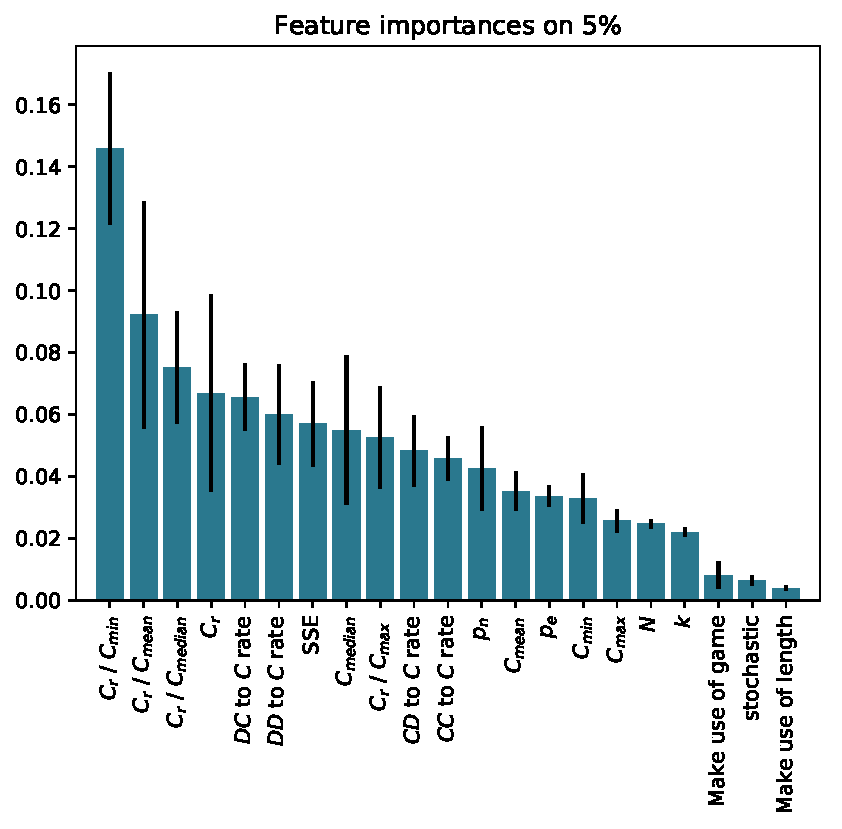
\includegraphics[width=.75\linewidth]{src/chapters/chapters-04/paper/axlml/new_output/probend_noise/_feature_importance_bar_plot_cluster_on_0_05.pdf}
        \end{center}
        \caption{Importance of features for clusters on 5\% performance.}
    \end{subfigure}
    \begin{subfigure}[t]{0.5\textwidth}
        \begin{center}
            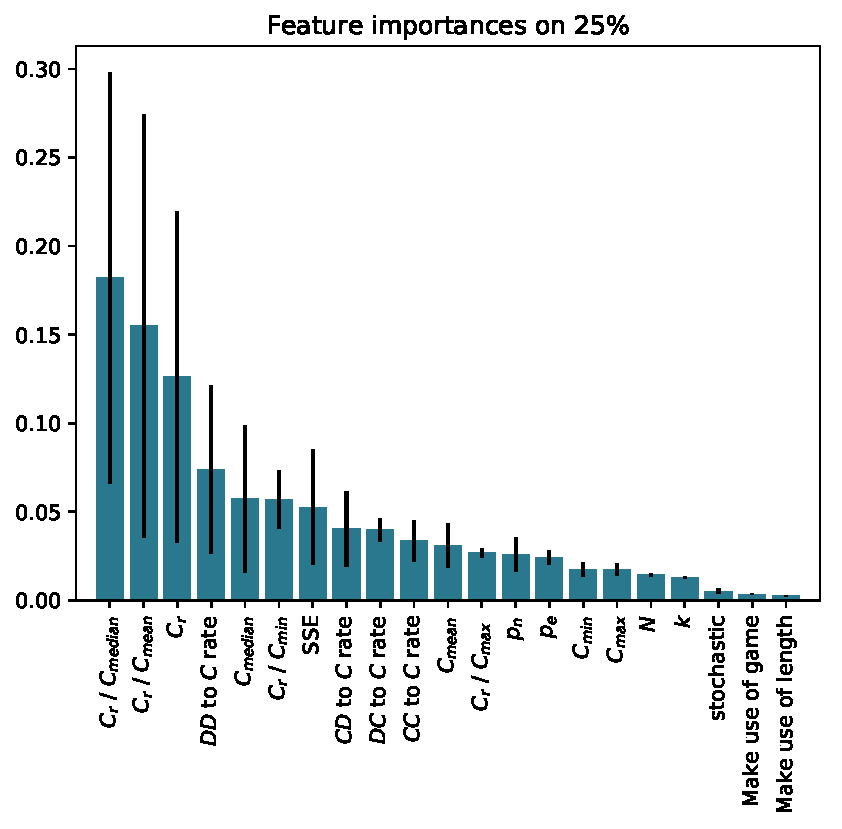
\includegraphics[width=.75\linewidth]{src/chapters/chapters-04/paper/axlml/new_output/probend_noise/_feature_importance_bar_plot_cluster_on_0_25.pdf}
        \end{center}
        \caption{Importance of features for clusters on 25\% performance.}
    \end{subfigure}
    \begin{subfigure}[t]{0.5\textwidth}
        \begin{center}
            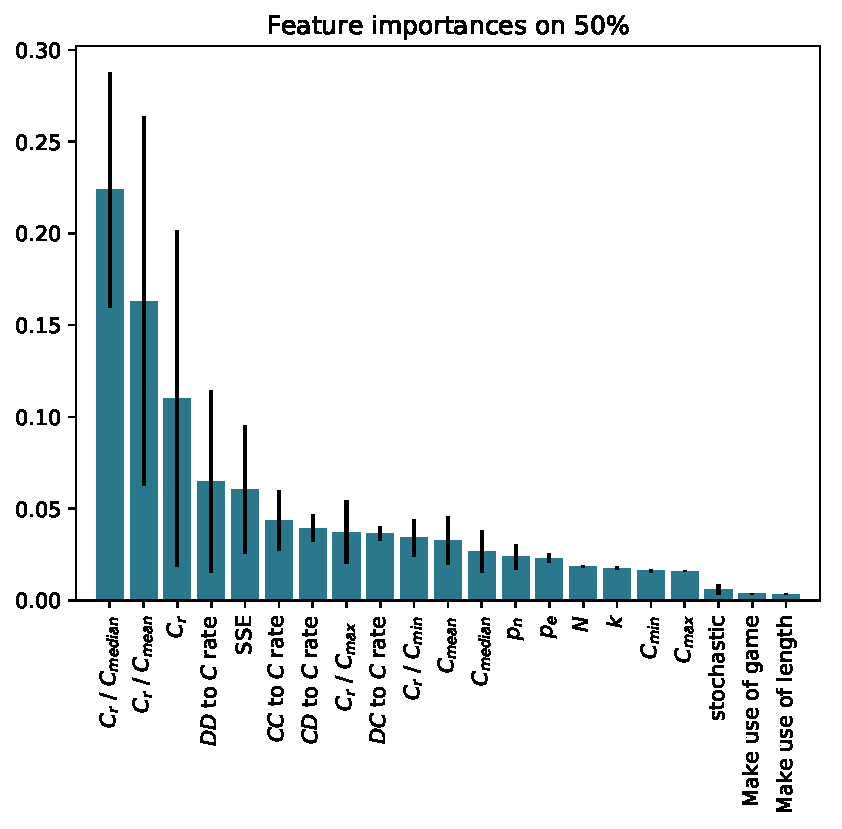
\includegraphics[width=.75\linewidth]{src/chapters/chapters-04/paper/axlml/new_output/probend_noise/_feature_importance_bar_plot_cluster_on_0_5.pdf}
        \end{center}
        \caption{Importance of features for clusters on 50\% performance.}
    \end{subfigure}
    \begin{subfigure}[t]{0.5\textwidth}
        \begin{center}
            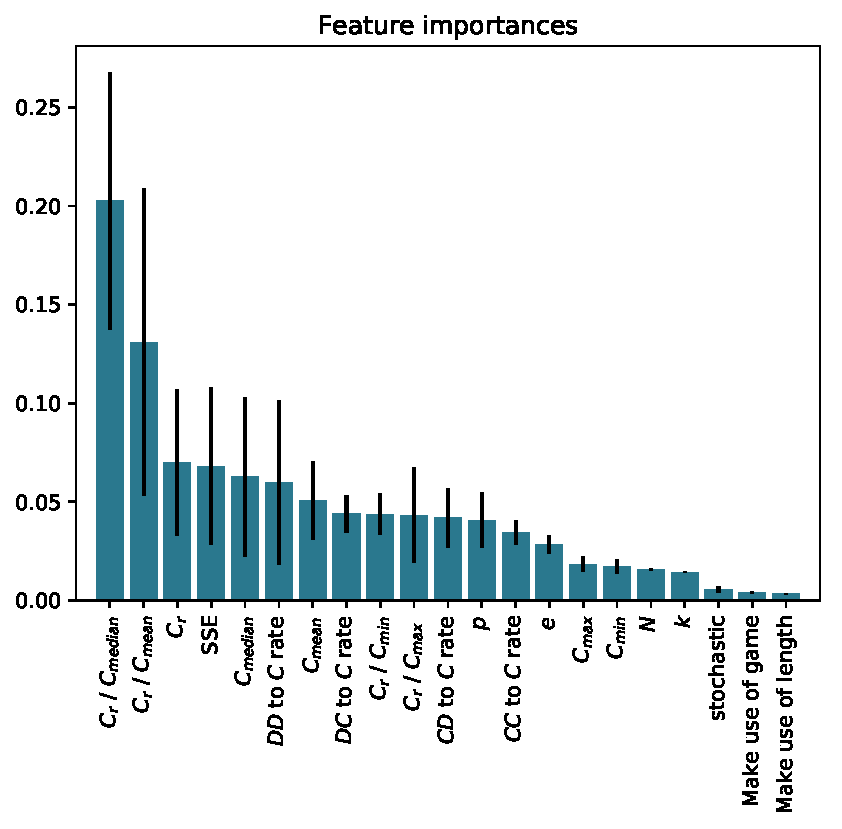
\includegraphics[width=.75\linewidth]{src/chapters/chapters-04/paper/axlml/k_means_output/probend_noise/_feature_importance_bar_plot.pdf}
        \end{center}
        \caption{Importance of features for clusters based on \(k\)means algorithm.}
    \end{subfigure}
    \caption{Importance of features in noisy probabilistic ending tournaments for different
    clustering methods.}\label{fig:clustering_importance_probend_noise}
\end{figure}

\begin{figure}[!htbp]
    \begin{subfigure}[t]{0.5\textwidth}
        \begin{center}
            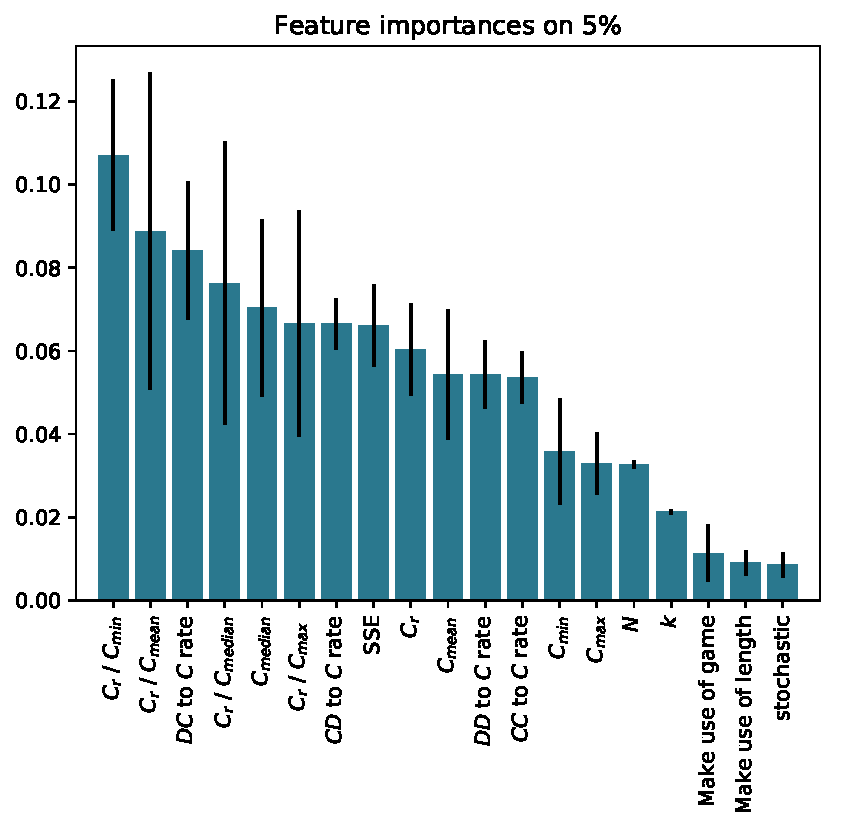
\includegraphics[width=.75\linewidth]{src/chapters/chapters-04/paper/axlml/new_output/merged/_feature_importance_bar_plot_cluster_on_0_05.pdf}
        \end{center}
        \caption{Importance of features for clusters on 5\% performance.}
    \end{subfigure}
    \begin{subfigure}[t]{0.5\textwidth}
        \begin{center}
            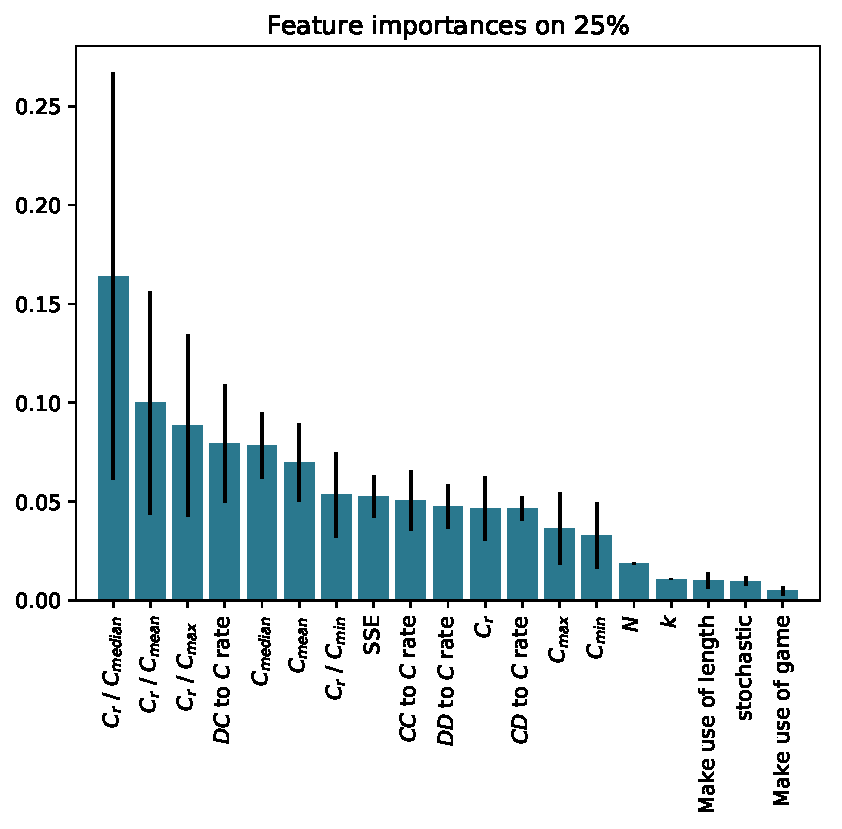
\includegraphics[width=.75\linewidth]{src/chapters/chapters-04/paper/axlml/new_output/merged/_feature_importance_bar_plot_cluster_on_0_25.pdf}
        \end{center}
        \caption{Importance of features for clusters on 25\% performance.}
    \end{subfigure}
    \begin{subfigure}[t]{0.5\textwidth}
        \begin{center}
            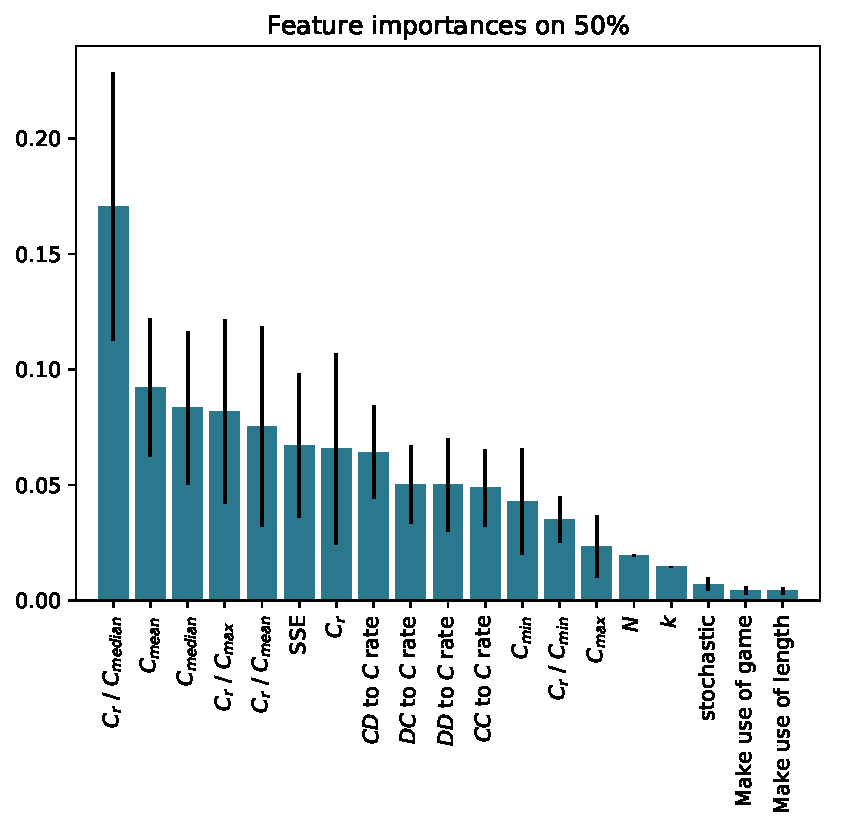
\includegraphics[width=.75\linewidth]{src/chapters/chapters-04/paper/axlml/new_output/merged/_feature_importance_bar_plot_cluster_on_0_5.pdf}
        \end{center}
        \caption{Importance of features for clusters on 50\% performance.}
    \end{subfigure}
    \begin{subfigure}[t]{0.5\textwidth}
        \begin{center}
            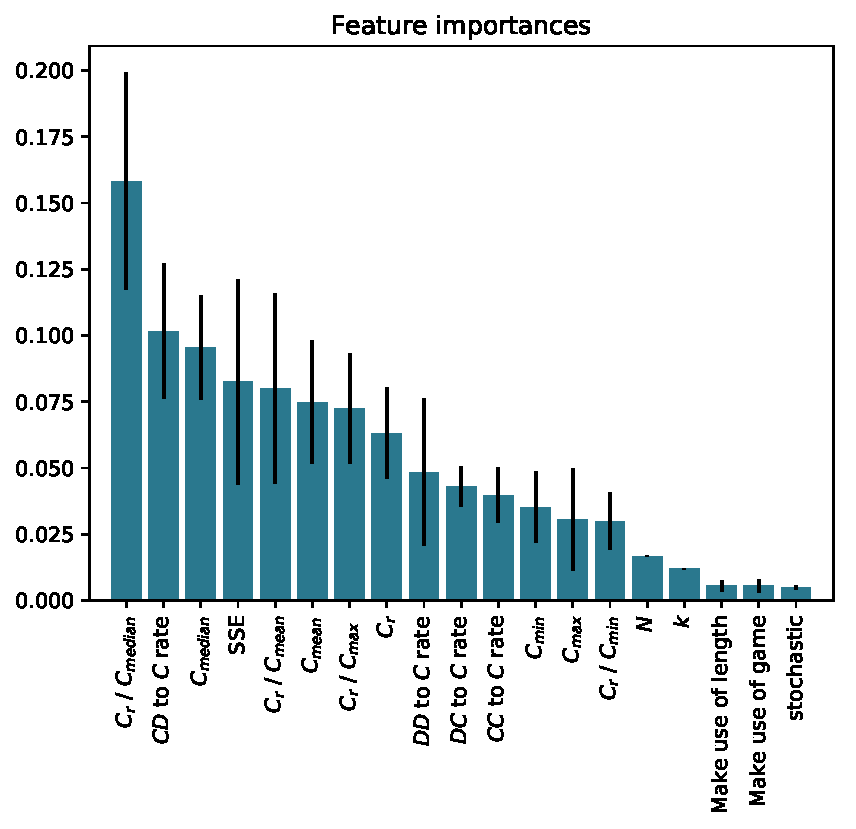
\includegraphics[width=.75\linewidth]{src/chapters/chapters-04/paper/axlml/k_means_output/merged/_feature_importance_bar_plot.pdf}
        \end{center}
        \caption{Importance of features for clusters based on \(k\)means algorithm.}
    \end{subfigure}
    \caption{Importance of features over all the tournaments for different
    clustering methods.}\label{fig:clustering_importance_overall}
\end{figure}

The effect of both these measures can be further explored. In
Figure~\ref{fig:mean_median_std} the distributions of \(C_r / C_{\text{mean}}\)
and \(C_r / C_{\text{median}}\) are given for the winners in standard tournaments. A value of \(C_r /
C_{\text{mean}} = 1\) imply that the cooperating ratio of the winner was the
same as the mean/median cooperating ratio of the tournament. In standard tournaments, the mean
for both ratios is 1. Therefore, an effective strategy in standard tournaments
was the mean/median cooperator of its respective tournament. In comparison,
Figure~\ref{fig:mean_median_noisy} shows the distributions of the measures for
the winners in noisy tournaments where the mean is at 0.67. Thereupon the winners
cooperated 67\% of the times the mean/median cooperator did. This analysis is
applied to the rest of the tournaments and the distributions are given by
Figures \ref{fig:mean_median_probend}, \ref{fig:mean_median_probend_noisy} and
\ref{fig:mean_median_overall}. In a tournament with noisy and a probabilistic
ending the winners cooperated 60\%, whereas in settings that the type of the
tournament can vary between the types considered in this work the winners
cooperated 67\% of the times the mean or median cooperator did. Finally, in
probabilistic ending tournament it has already been mentioned that defecting
strategies prevail and this result is once again confirmed in this section.

\begin{figure}[!htbp]
    \centering
    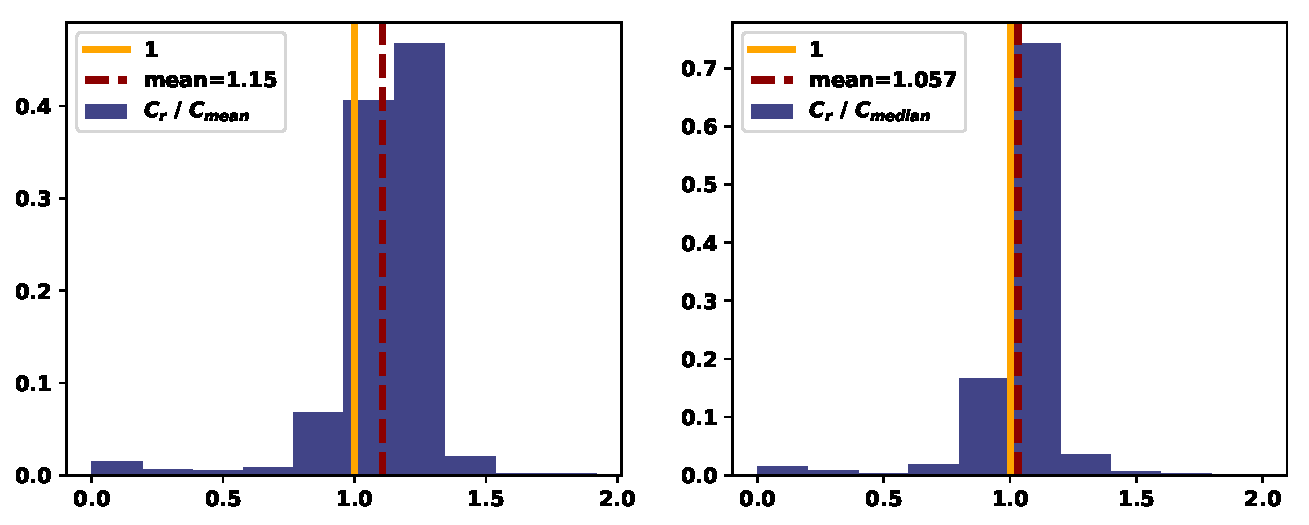
\includegraphics[width=.5\textwidth]{src/chapters/chapters-04/paper/axlml/images/compared_to_mean_median_standard.pdf}
    \caption{Distributions of \(C_r / C_{\text{median}}\)
    and \(C_r / C_{\text{median}}\) for winners of standard tournaments.}\label{fig:mean_median_std}
\end{figure}

\begin{figure}[!htbp]
    \centering
    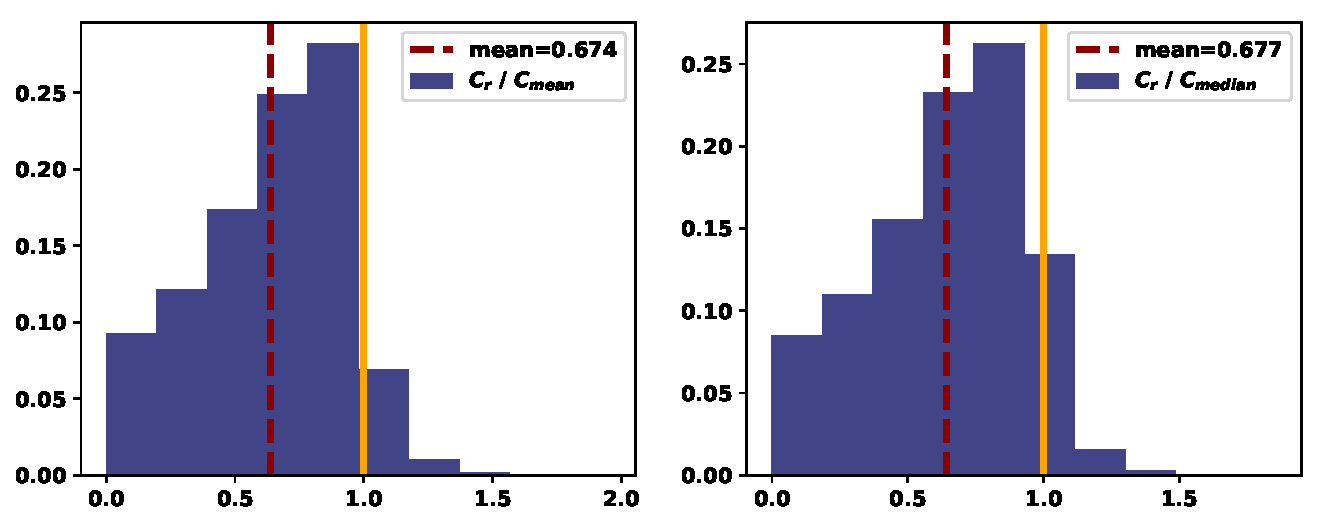
\includegraphics[width=.5\textwidth]{src/chapters/chapters-04/paper/axlml/images/compared_to_mean_median_noisy.pdf}
    \caption{Distributions of \(C_r / C_{\text{median}}\)
    and \(C_r / C_{\text{median}}\) for winners of noisy tournaments.}\label{fig:mean_median_noisy}
\end{figure}

\begin{figure}[!htbp]
    \centering
    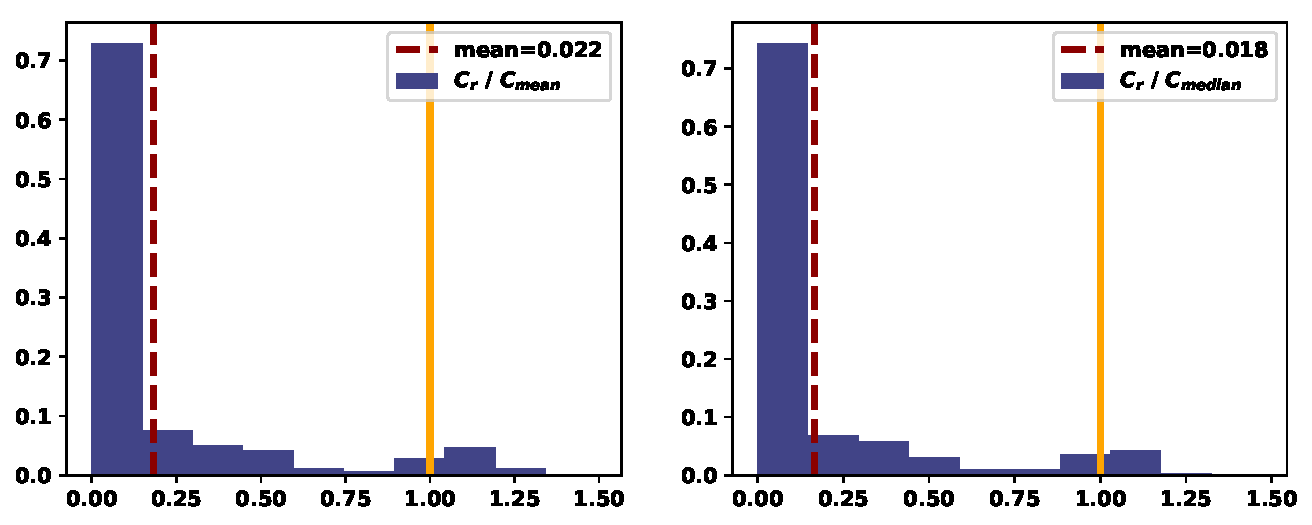
\includegraphics[width=.5\textwidth]{src/chapters/chapters-04/paper/axlml/images/compared_to_mean_median_probend.pdf}
    \caption{Distributions of \(C_r / C_{\text{median}}\)
    and \(C_r / C_{\text{median}}\) for winners of probabilistic ending tournaments.}\label{fig:mean_median_probend}
\end{figure}

\begin{figure}[!htbp]
    \centering
    \includegraphics[width=.5\textwidth]{src/chapters/chapters-04/paper/axlml/images/compared_to_mean_median_probend_noisy.pdf}
    \caption{Distributions of \(C_r / C_{\text{median}}\)
    and \(C_r / C_{\text{median}}\) for winners of noisy probabilistic ending tournaments.}\label{fig:mean_median_probend_noisy}
\end{figure}

\begin{figure}[!htbp]
    \centering
    \includegraphics[width=.5\textwidth]{src/chapters/chapters-04/paper/axlml/images/compared_to_mean_median_overall.pdf}
    \caption{Distributions of \(C_r / C_{\text{median}}\)
    and \(C_r / C_{\text{median}}\) for winners of over all the tournaments.}\label{fig:mean_median_overall}
\end{figure}

In this section the effect of several measures, regarding a strategy's behaviour
and the tournament in which it participated on its performance were presented.
This was done using two approaches. Correlation coefficients and a random forest
analysis. The results of these are summarised in the following section.

\section{Conclusion}\label{section:conclusion}

This manuscript has explored the performance of \numberofstrategies strategies of the Iterated
Prisoner's Dilemma in a large number of computer tournaments. The results of
the analysis demonstrated that, although for specific tournament types such as
standard and probabilistic ending tournaments, dominant strategies exist
there is not a single dominant type of strategies if the environments
vary. Moreover, a strategy with a theory of mind should aim to adapt its behaviour
based on the mean and median cooperators.

The \numberofstrategies strategies used in this manuscript have been mainly for
the literature, and they have been accessible due to an open source software
called Axelrod-Python. The software was used to generate a total of
\numberofalltournaments computer tournaments results with different number of
strategies and different participants each time. The data collection was
described in Section~\ref{section:data_collection}. In
Section~\ref{section:top_performances}, the tournaments results were used to
present the top performances. The data set contained results from four different
settings, and these were also studied individually. In standard tournaments
complex strategies trained using reinforcement learning ranked in the top spots.
Some of these strategies ranked again in the top spots in probabilistic
ending tournaments when a \(p_e\) of less 0.1 was considered. In probabilistic
ending tournaments \(p_e\) was designed to vary between 0 and 1. It was demonstrated
that for values larger than 0.1, as stated in the Folk Theorem, defecting strategies
were winning the tournaments because there was a high likelihood of the game
ending in the next turn. In tournaments with noise the median ranks of the top
15 strategies had the highest values and the \(r\) distributions were bimodal.
The top rank strategies were performing both well and bad, and this indicates
that in noisy tournaments there are not strategies that can guarantee winning.
Overall, the top ranked strategies differed from one tournament type to
another and the mechanism behind the winning strategies were all different.
Even strategies designed to do good in one setting did better in others.
On the whole ... (the ipd interactions are unique and there is no winning
strategy) %TODO help from Vince

Section~\ref{section:evaluation_of_performance}, covered an analysis of
performance based on several measures associated with a strategy and with the
environments it was competing. The results of this analysis showed that a
strategy's characteristics such as whether or not it's stochastic, and the information it
used regarding the game had no effect on the strategy's success. The most
important factors have been those that compared the strategy's behaviour to it's
environment. The cooperating ratio of the strategy compared to the mean and
median cooperator was highlighted as the most important feature in the analysis.
More specifically, if a strategy were to enter a tournament with a theory of
mind of its environment it would choose to be the median cooperator in standard
tournaments, to cooperate 10\% in probabilistic ending tournaments and 
60\% in noisy and noisy probabilistic
tournaments of the times the median cooperator did. Lastly, if a strategy was aware of the opponents but not of the
setting on the tournament, a strategy would be more likely to be successful if
it were to identify the median cooperator and cooperated 67\% of the times that
they did.

The data set described in this work contains the largest number of IPD tournaments,
to the authors knowledge, and it available at~\cite{data}. Further data mining
could be applied and provide new insights in the field.

% \bibliographystyle{plain}
% \bibliography{bibliography}

% \section{Acknowledgements}

% A variety of software have been used in this work:

% \begin{itemize}
%     \item The Axelrod library for IPD simulations~\cite{axelrodproject}.
%     \item The Matplotlib library for visualisation~\cite{hunter2007matplotlib}.
%     \item The Numpy library for data manipulation~\cite{walt2011numpy}.
%     \item The scikit-learn library for data analysis~\cite{scikit-learn}.
% \end{itemize}

% \appendix

\section{A summary of parameters}\label{app:parameters}

\begin{table}[h]
    \begin{center}
    \resizebox{.7\textwidth}{!}{
    \begin{tabular}{llc}
    \toprule
measure & measure explanation \\
 \midrule
stochastic                  & If a strategy is stochastic \\
makes use of game           & If a strategy makes used of the game information  \\
makes use of length         & If a strategy makes used of the number of turns \\
memory usage                & The memory size of a strategy divided by the number of turns \\
SSE                         & A measure of how far a strategy is from extortionate behaviour \\
$C_{\text{max}}$          & The biggest cooperating rate in the tournament \\
$C_{\text{min}}$          & The smallest cooperating rate in the tournament \\
$C_{\text{median}}$       & The median cooperating rate in the tournament \\
$C_{\text{mean}}$         & The mean cooperating rate in the tournament \\
$C_r$ / $C_{\text{max}}$    & A strategy's cooperating rate divided by the maximum \\
$C_r$ / $C_{\text{min}}$    & A strategy's cooperating rate divided by the minimum \\
$C_r$ / $C_{\text{median}}$ & A strategy's cooperating rate divided by the median \\
$C_r$ / $C_{\text{mean}}$   & A strategy's cooperating rate divided by the mean \\
$C_r$                       & The cooperating ratio of a strategy \\
$CC$ to $C$ rate            & The probability a strategy will cooperate after a mutual cooperation \\
$CD$ to $C$ rate            & The probability a strategy will cooperate after being betrayed by the opponent \\
$DC$ to $C$ rate            & The probability a strategy will cooperate after betraying the opponent\\
$DD$ to $C$ rate            & The probability a strategy will cooperate after a mutual defection\\
$p_n$                       & The probability of a player's action being flip at each interaction \\
$n$                         & The number of turns \\
$p_e$                       & The probability of a match ending in the next turn \\
$N$                         & The number of strategies in the tournament \\
$k$                         & The number that a given tournament is repeated \\
    \bottomrule
        \end{tabular}}
    \end{center}
    \caption{The measures which are included in the performance evaluation analysis.}
\end{table}



\section{List of strategies}\label{app:list_of_players}

The strategies used in this study which are from Axelrod version 3.0.0
\cite{axelrodproject}.

\begin{multicols}{3}
	\begin{enumerate}
		\item $\phi$~\cite{axelrodproject}
\item $\pi$~\cite{axelrodproject}
\item $e$~\cite{axelrodproject}
\item ALLCorALLD \cite{axelrodproject}
\item Adaptive~\cite{Li2011}
\item Adaptive Pavlov 2006~\cite{kendall2007iterated}
\item Adaptive Pavlov 2011~\cite{Li2011}
\item Adaptive Tit For Tat: 0.5~\cite{Tzafestas2000}
\item Aggravater~\cite{axelrodproject}
\item Alexei~\cite{lesswrong}
\item Alternator~\cite{Axelrod1981, Mittal2009}
\item Alternator Hunter~\cite{axelrodproject}
\item Anti Tit For Tat~\cite{Hilbe2013}
\item AntiCycler~\cite{axelrodproject}
\item Appeaser~\cite{axelrodproject}
\item Arrogant QLearner~\cite{axelrodproject}
\item Average Copier~\cite{axelrodproject}
\item Backstabber~\cite{axelrodproject}
\item Better and Better~\cite{prison}
\item Bully~\cite{Nachbar1992}
\item Calculator~\cite{prison}
\item Cautious QLearner~\cite{axelrodproject}
\item Champion~\cite{Axelrod1980b}
\item CollectiveStrategy~\cite{Li2009}
\item Contrite Tit For Tat~\cite{Axelrod1995}
\item Cooperator~\cite{Axelrod1981, Mittal2009, Press2012}
\item Cooperator Hunter~\cite{axelrodproject}
\item Cycle Hunter~\cite{axelrodproject}
\item Cycler CCCCCD~\cite{axelrodproject}
\item Cycler CCCD~\cite{axelrodproject}
\item Cycler CCCDCD~\cite{axelrodproject}
\item Cycler CCD~\cite{Mittal2009}
\item Cycler DC~\cite{axelrodproject}
\item Cycler DDC~\cite{Mittal2009}
\item DBS~\cite{Au2006}
\item Davis~\cite{Axelrod1980a}
\item Defector~\cite{Axelrod1981, Mittal2009, Press2012}
\item Defector Hunter~\cite{axelrodproject}
\item Double Crosser~\cite{axelrodproject}
\item Desperate \cite{Van2015}
\item DoubleResurrection~\cite{Eckhart2015}
\item Doubler~\cite{prison}
\item Dynamic Two Tits For Tat~\cite{axelrodproject}
\item EasyGo~\cite{Li2011, prison}
\item Eatherley~\cite{Axelrod1980b}
\item Eventual Cycle Hunter~\cite{axelrodproject}
\item Evolved ANN~\cite{axelrodproject}
\item Evolved ANN 5~\cite{axelrodproject}
\item Evolved ANN 5 Noise 05~\cite{axelrodproject}
\item Evolved FSM 16~\cite{axelrodproject}
\item Evolved FSM 16 Noise 05~\cite{axelrodproject}
\item Evolved FSM 4~\cite{axelrodproject}
\item Evolved HMM 5~\cite{axelrodproject}
\item EvolvedLookerUp1 1 1~\cite{axelrodproject}
\item EvolvedLookerUp2 2 2~\cite{axelrodproject}
\item Eugine Nier~\cite{lesswrong}
\item Feld~\cite{Axelrod1980a}
\item Firm But Fair~\cite{Frean1994}
\item Fool Me Forever~\cite{axelrodproject}
\item Fool Me Once~\cite{axelrodproject}
\item Forgetful Fool Me Once~\cite{axelrodproject}
\item Forgetful Grudger~\cite{axelrodproject}
\item Forgiver~\cite{axelrodproject}
\item Forgiving Tit For Tat~\cite{axelrodproject}
\item Fortress3~\cite{Ashlock2006}
\item Fortress4~\cite{Ashlock2006}
\item GTFT \cite{Gaudesi2016, Nowak1993}
\item General Soft Grudger~\cite{axelrodproject}
\item Gradual~\cite{Beaufils1997}
\item Gradual Killer~\cite{prison}
\item Grofman\cite{Axelrod1980a}
\item Grudger~\cite{Axelrod1980a, Banks1990, Beaufils1997, Van2015, Li2011}
\item GrudgerAlternator~\cite{prison}
\item Grumpy~\cite{axelrodproject}
\item Handshake~\cite{Robson1990}
\item Hard Go By Majority~\cite{Mittal2009}
\item Hard Go By Majority: 10~\cite{axelrodproject}
\item Hard Go By Majority: 20~\cite{axelrodproject}
\item Hard Go By Majority: 40~\cite{axelrodproject}
\item Hard Go By Majority: 5~\cite{axelrodproject}
\item Hard Prober~\cite{prison}
\item Hard Tit For 2 Tats~\cite{Stewart2012}
\item Hard Tit For Tat~\cite{PD2017}
\item Hesitant QLearner\cite{axelrodproject}
\item Hopeless~\cite{Van2015}
\item Inverse~\cite{axelrodproject}
\item Inverse Punisher~\cite{axelrodproject}
\item Joss~\cite{Axelrod1980a, Stewart2012}
\item Knowledgeable Worse and Worse~\cite{axelrodproject}
\item Level Punisher~\cite{Eckhart2015}
\item Limited Retaliate 2~\cite{axelrodproject}
\item Limited Retaliate 3~\cite{axelrodproject}
\item Limited Retaliate~\cite{axelrodproject}
\item MEM2~\cite{Li2014}
\item Math Constant Hunter~\cite{axelrodproject}
\item Meta Hunter Aggressive~\cite{axelrodproject}
\item Meta Hunter~\cite{axelrodproject}
\item Meta Majority~\cite{axelrodproject}
\item Meta Majority Finite Memory~\cite{axelrodproject}
\item Meta Majority Long Memory~\cite{axelrodproject}
\item Meta Majority Memory One~\cite{axelrodproject}
\item Meta Minority~\cite{axelrodproject}
\item Meta Mixer~\cite{axelrodproject}
\item Meta Winner~\cite{axelrodproject}
\item Meta Winner Deterministic~\cite{axelrodproject}
\item Meta Winner Ensemble~\cite{axelrodproject}
\item Meta Winner Finite Memory~\cite{axelrodproject}
\item Meta Winner Long Memory~\cite{axelrodproject}
\item Meta Winner Memory One~\cite{axelrodproject}
\item Meta Winner Stochastic~\cite{axelrodproject}
\item NMWE Deterministic~\cite{axelrodproject}
\item NMWE Finite Memory~\cite{axelrodproject}
\item NMWE Long Memory~\cite{axelrodproject}
\item NMWE Memory One~\cite{axelrodproject}
\item NMWE Stochastic~\cite{axelrodproject}
\item Naive Prober~\cite{Li2011}
\item Negation~\cite{PD2017}
\item Nice Average Copier~\cite{axelrodproject}
\item Nice Meta Winner~\cite{axelrodproject}
\item Nice Meta Winner Ensemble~\cite{axelrodproject}
\item Nydegger~\cite{Axelrod1980a}
\item Omega TFT~\cite{kendall2007iterated}
\item Once Bitten~\cite{axelrodproject}
\item Opposite Grudger~\cite{axelrodproject}
\item PSO Gambler 1 1 1~\cite{axelrodproject}
\item PSO Gambler 2 2 2~\cite{axelrodproject}
\item PSO Gambler 2 2 2 Noise 05~\cite{axelrodproject}
\item PSO Gambler Mem1 \cite{axelrodproject}
\item Predator~\cite{Ashlock2006}
\item Prober~\cite{Li2011}
\item Prober 2~\cite{prison}
\item Prober 3~\cite{prison}
\item Prober 4~\cite{prison}
\item Pun1~\cite{Ashlock2006}
\item Punisher~\cite{axelrodproject}
\item Raider~\cite{Ashlock2014}
\item Random Hunter~\cite{axelrodproject}
\item Random: 0.5~\cite{Axelrod1980a, Tzafestas2000}
\item Remorseful Prober~\cite{Li2011}
\item Resurrection~\cite{Eckhart2015}
\item Retaliate 2~\cite{axelrodproject}
\item Retaliate 3~\cite{axelrodproject}
\item Retaliate~\cite{axelrodproject}
\item Revised Downing~\cite{Axelrod1980a}
\item Ripoff~\cite{Ashlock2008}
\item Risky QLearner~\cite{axelrodproject}
\item SelfSteem~\cite{Andre2013}
\item ShortMem ~\cite{Andre2013}
\item Shubik~\cite{Axelrod1980a}
\item Slow Tit For Two Tats~\cite{axelrodproject}
\item Slow Tit For Two Tats 2~\cite{prison}
\item Sneaky Tit For Tat~\cite{axelrodproject}
\item Soft Go By Majority~\cite{Axelrod1981, Mittal2009}
\item Soft Go By Majority 10~\cite{axelrodproject}
\item Soft Go By Majority 20~\cite{axelrodproject}
\item Soft Go By Majority 40~\cite{axelrodproject}
\item Soft Go By Majority 5~\cite{axelrodproject}
\item Soft Grudger~\cite{Li2011}
\item Soft Joss~\cite{prison}
\item SolutionB1~\cite{Ashlock2015}
\item SolutionB5~\cite{Ashlock2015}
\item Spiteful Tit For Tat~\cite{prison}
\item Stalker~\cite{Carvalho2013}
\item Stein and Rapoport~\cite{Axelrod1980a}
\item Stochastic Cooperator~\cite{Adami2013}
\item Stochastic WSLS~\cite{axelrodproject}
\item Suspicious Tit For Tat~\cite{Beaufils1997, Hilbe2013}
\item TF1~\cite{axelrodproject}
\item TF2~\cite{axelrodproject}
\item TF3~\cite{axelrodproject}
\item Tester~\cite{Axelrod1980b}
\item ThueMorse~\cite{axelrodproject}
\item ThueMorseInverse~\cite{axelrodproject}
\item Thumper~\cite{Ashlock2008}
\item Tit For 2 Tats (\textbf{Tf2T})~\cite{Axelrod1981}
\item Tit For Tat (\textbf{TfT})~\cite{Axelrod1980a}
\item Tricky Cooperator~\cite{axelrodproject}
\item Tricky Defector~\cite{axelrodproject}
\item Tullock~\cite{Axelrod1980a}
\item Two Tits For Tat (\textbf{2TfT})~\cite{Axelrod1981}
\item VeryBad~\cite{Andre2013}
\item Willing \cite{Van2015}
\item Win-Shift Lose-Stay (\textbf{WShLSt})~\cite{Li2011}
\item Win-Stay Lose-Shift (\textbf{WSLS})~\cite{Kraines1989, Nowak1993, Stewart2012}
\item Winner12~\cite{mathieu2017}
\item Winner21~\cite{mathieu2017}
\item Worse and Worse\cite{prison}
\item Worse and Worse 2\cite{prison}
\item Worse and Worse 3\cite{prison}
\item ZD-Extort-2 v2~\cite{Kuhn2017}
\item ZD-Extort-2~\cite{Stewart2012}
\item ZD-Extort-4~\cite{axelrodproject}
\item ZD-GEN-2~\cite{Kuhn2017}
\item ZD-GTFT-2~\cite{Stewart2012}
\item ZD-SET-2~\cite{Kuhn2017}
	\end{enumerate}
\end{multicols}


\section{Correlation coefficients}\label{app:correlations}

A graphical representation of the correlation coefficients for the measures in
Table~\ref{table:manual_measures}.

\begin{figure}[!htbp]
        \begin{center}
            \includegraphics[width=.75\linewidth]{src/chapters/chapters-04/paper/axlml/images/standard_correlation_plot.pdf}
        \end{center}
        \caption{Correlation coefficients of measures in Table~\ref{table:manual_measures}
        for standard tournaments}
\end{figure}
\begin{figure}[!htbp]
    \begin{center}
        \includegraphics[width=.75\linewidth]{src/chapters/chapters-04/paper/axlml/images/noise_correlation_plot.pdf}
    \end{center}
    \caption{Correlation coefficients of measures in Table~\ref{table:manual_measures}
    for noisy tournaments}
\end{figure}
\begin{figure}[!htbp]
    \begin{center}
        \includegraphics[width=.75\linewidth]{src/chapters/chapters-04/paper/axlml/images/probend_correlation_plot.pdf}
    \end{center}
    \caption{Correlation coefficients of measures in Table~\ref{table:manual_measures}
    for probabilistic ending tournaments}
\end{figure}
\begin{figure}[!htbp]
    \begin{center}
        \includegraphics[width=.75\linewidth]{src/chapters/chapters-04/paper/axlml/images/probend_noise_correlation_plot.pdf}
    \end{center}
    \caption{Correlation coefficients of measures in Table~\ref{table:manual_measures}
    for noisy probabilistic ending tournaments}
\end{figure}
\begin{figure}[!htbp]
    \begin{center}
        \includegraphics[width=.75\linewidth]{src/chapters/chapters-04/paper/axlml/images/merged_correlation_plot.pdf}
    \end{center}
    \caption{Correlation coefficients of measures in Table~\ref{table:manual_measures}
    for data set}
\end{figure}

\chapter{Stability of defection, optimisation of strategies and the limits of
       memory in the Prisoner's Dilemma.}


Memory-one strategies are a set of Iterated Prisoner's Dilemma strategies
that have been praised for their mathematical tractability and performance
against single opponents. This manuscript investigates \textit{best
response} memory-one strategies as a multidimensional
optimisation problem. Though extortionate memory-one strategies have gained
much attention, we demonstrate that best response memory-one strategies do not
behave in an extortionate way, and moreover, for memory one strategies to be
evolutionary robust they need to be able to behave in a forgiving way. We
also provide evidence that memory-one strategies suffer from their limited
memory in multi agent interactions and can be out performed by
longer memory strategies.

\section{Introduction}\label{section:introduction}

The Prisoner's Dilemma (PD) is a two player game used in understanding the
evolution of cooperative behaviour, formally introduced in~\cite{Flood1958}.
Each player has two options, to cooperate (C) or to defect (D). The decisions
are made simultaneously and independently. The normal form representation of the
game is given by:

\begin{equation}\label{equ:pd_definition}
    S_p =
    \begin{pmatrix}
        R & S  \\
        T & P
    \end{pmatrix}
    \quad
    S_q =
    \begin{pmatrix}
        R & T  \\
        S & P
    \end{pmatrix}
\end{equation}

where \(S_p\) represents the utilities of the row player and \(S_q\) the
utilities of the column player. The payoffs, \((R, P, S, T)\), are constrained
by equations~(\ref{eq:pd_constrain_one}) and~(\ref{eq:pd_constrain_two}).
Constraint~(\ref{eq:pd_constrain_one}) ensures that
defection dominates cooperation and constraint~(\ref{eq:pd_constrain_two})
ensures that there is a dilemma; the sum of the utilities for both players is
better when both choose to cooperate. The most common values used in the literature are
\((R, P, S, T) = (3, 1, 0, 5)\)~\cite{Axelrod1981}.


\begin{equation}\label{eq:pd_constrain_one}
    T > R > P > S
\end{equation}

\begin{equation}\label{eq:pd_constrain_two}
    2R > T + S
\end{equation}

The PD is a one shot game, however, it is commonly studied in a manner where the
history of the interactions matters. The repeated form of the game is called the
Iterated Prisoner's Dilemma (IPD) and in the 1980s, following the work
of~\cite{Axelrod1980a, Axelrod1980b} it attracted the attention of the
scientific community. In~\cite{Axelrod1980a} and~\cite{Axelrod1980b}, the first
well known computer tournaments of the IPD were performed. A total of 13 and 62
strategies were submitted respectively in the form of computer code. The
contestants competed against each other, a copy of themselves and a random
strategy, and the winner was then decided on the average score achieved (not the
total number of wins). The contestants were given access to the entire history
of a match, however, how many turns of history a strategy would incorporate,
referred to as the \textit{memory size} of a strategy, was a result of the
particular strategic decisions made by the author. The winning strategy of both
tournaments was a strategy called Tit for Tat and its success in both
tournaments came as a surprise. Tit for Tat was a simple, forgiving strategy
that opened each interaction by cooperation, and had won the tournament even
though it never scored higher than that its direct opponent. Tit for Tat provided
evidence that being nice can be advantageous and became the major paradigm for
reciprocal altruism.

Another trait of Tit for Tat is that it considers only the previous move of the
opponent. These type of strategies are called \textit{reactive} \cite{Nowak1989}
and are a subset of so called \textit{memory-one} strategies, which incorporate
both players' latests moves. Memory-one strategies have been
studied thoroughly in the literature~\cite{Nowak1990, Nowak1993}, however, they have gained
most of their attention when a certain subset of memory-one strategies was
introduced in~\cite{Press2012}, the zero-determinants. In~\cite{Stewart2012} it
was stated that ``Press and Dyson have fundamentally changed the viewpoint on
the Prisoner's Dilemma''.
Zero-determinants are a special case of memory-one and extortionate
strategies. They choose their actions so that a linear relationship is forced
between the players' score ensuring that they will always
receive at least as much as their opponents. Zero-determinants are
indeed mathematically unique and are proven to be robust in pairwise
interactions, however, their true effectiveness in tournaments and
evolutionary dynamics has been questioned~\cite{adami2013, Hilbe2013b,
Hilbe2013, Hilbe2015, Knight2018, Harper2015}.

In a similar fashion to~\cite{Press2012} the purpose of this work is to consider
a given memory-one strategy; however, whilst~\cite{Press2012} found a way for a
player to manipulate a given opponent, this work will consider a
multidimensional optimisation approach to identify the best response to a given
group of opponents. In particular, this work presents a compact method of
identifying the best response memory-one strategy against a given set of
opponents, and evaluates whether it behaves extortionately, similar to
zero-determinants. Further theoretical and empirical results of this work
include:

\begin{enumerate}
    \item The conditions that ensure a best response memory-one strategy evolutionary
    robust.
    \item A well designed framework that allows the comparison of an optimal
          memory one strategy and a more complex strategy which has a larger
          memory and was obtained through reinforcement learning
          techniques~\cite{Harper2017}.
    \item An identification of conditions for which defection is known to be
    stable; thus identifying environments where cooperation will not
    occur.
\end{enumerate}

\section{The utility}\label{section:utility}

One specific advantage of memory-one strategies is their mathematical
tractability. They can be represented completely as an element of \(\R^{4}_{[0, 1]}\). This
originates from~\cite{Nowak1989} where it is stated that if a strategy is
concerned with only the outcome of a single turn then there are four possible
`states' the strategy could be in;

\begin{itemize}
    \item both players cooperated, denoted as \(CC\)
    \item first players cooperated whilst the second player defected, denoted as \(CD\)
    \item first players defected whilst the second player cooperated, denoted as \(DC\)
    \item both players defected, denoted as \(DD\)
\end{itemize}

Therefore, a memory-one strategy can be denoted by the probability vector of
cooperating after each of these states; \(p=(p_1, p_2, p_3, p_4) \in \R_{[0,1]}
^ 4\).

In~\cite{Nowak1989} it was shown that it is not necessary to simulate the play
of a strategy $p$ against a memory-one opponent $q$. Rather this exact behaviour
can be modeled as a stochastic process, and more specifically as a Markov chain
(Figure~\ref{fig:markov_chain}) whose corresponding transition matrix \(M\) is
given by (\ref{eq:transition_matrix}). The long run steady state probability
vector \(v\), which is the solution to \(v M = v\), can be
combined with the payoff matrices of (\ref{equ:pd_definition}) to give the expected
payoffs for each player. More specifically, the utility for a memory-one
strategy \(p\) against an opponent \(q\), denoted as \(u_q(p)\), is given by
(\ref{eq:press_dyson_utility}).

\begin{figure}
    \centering
    \includestandalone[width=.35\textwidth]{src/chapters/chapters-05/paper/Memory-size-in-the-prisoners-dilemma/tex/markov_chain}
    \caption{Markov Chain}
    \label{fig:markov_chain}
\end{figure}

\begin{equation}\label{eq:transition_matrix}
    M = \left[\begin{matrix}p_{1} q_{1} & p_{1} \left(- q_{1} + 1\right) & q_{1} \left(- p_{1} + 1\right) & \left(- p_{1} + 1\right) \left(- q_{1} + 1\right)\\p_{2} q_{3} & p_{2} \left(- q_{3} + 1\right) & q_{3} \left(- p_{2} + 1\right) & \left(- p_{2} + 1\right) \left(- q_{3} + 1\right)\\p_{3} q_{2} & p_{3} \left(- q_{2} + 1\right) & q_{2} \left(- p_{3} + 1\right) & \left(- p_{3} + 1\right) \left(- q_{2} + 1\right)\\p_{4} q_{4} & p_{4} \left(- q_{4} + 1\right) & q_{4} \left(- p_{4} + 1\right) & \left(- p_{4} + 1\right) \left(- q_{4} + 1\right)\end{matrix}\right]
\end{equation}


\begin{equation}\label{eq:press_dyson_utility}
    u_q(p) = v \cdot (R, S, T, P).
\end{equation}

This manuscript has explored the form of \(u_q(p)\), to the authors knowledge no
previous work has done this, and it proves that \(u_q(p)\) is given by a ratio
of two quadratic forms~\cite{kepner2011},
Theorem~\ref{theorem:quadratic_form_u}.

\begin{theorem}\label{theorem:quadratic_form_u}
    The expected utility of a memory-one strategy \(p\in\mathbb{R}_{[0,1]}^4\)
    against a memory-one opponent \(q\in\mathbb{R}_{[0,1]}^4\), denoted
    as \(u_q(p)\), can be written as a ratio of two quadratic forms:

    \begin{equation}\label{eq:optimisation_quadratic}
    u_q(p) = \frac{\frac{1}{2}pQp^T + cp + a}
                {\frac{1}{2}p\bar{Q}p^T + \bar{c}p + \bar{a}},
    \end{equation}
    where \(Q, \bar{Q}\) \(\in \R^{4\times4}\) are square matrices defined by the
    transition probabilities of the opponent \(q_1, q_2, q_3, q_4\) as follows:

    \begin{center}
    \begin{equation}
    \resizebox{0.9\linewidth}{!}{\arraycolsep=2.5pt%
    \boldmath\(
    Q = \left[\begin{matrix}0 & - \left(q_{1} - q_{3}\right) \left(q_{2} - 5 q_{4} - 1\right) & q_{3} \left(q_{1} - q_{2}\right) & - 5 q_{3} \left(q_{1} - q_{4}\right)\\- \left(q_{1} - q_{3}\right) \left(q_{2} - 5 q_{4} - 1\right) & 0 & \left(q_{2} - q_{3}\right) \left(q_{1} - 3 q_{4} - 1\right) & \left(q_{3} - q_{4}\right) \left(5 q_{1} - 3 q_{2} - 2\right)\\q_{3} \left(q_{1} - q_{2}\right) & \left(q_{2} - q_{3}\right) \left(q_{1} - 3 q_{4} - 1\right) & 0 & 3 q_{3} \left(q_{2} - q_{4}\right)\\- 5 q_{3} \left(q_{1} - q_{4}\right) & \left(q_{3} - q_{4}\right) \left(5 q_{1} - 3 q_{2} - 2\right) & 3 q_{3} \left(q_{2} - q_{4}\right) & 0\end{matrix}\right]\)},
    \end{equation}
    \begin{equation}\label{eq:q_bar_matrix}
    \resizebox{0.8\linewidth}{!}{\arraycolsep=2.5pt%
    \boldmath\(
    \bar{Q} =  \left[\begin{matrix}0 & - \left(q_{1} - q_{3}\right) \left(q_{2} - q_{4} - 1\right) & \left(q_{1} - q_{2}\right) \left(q_{3} - q_{4}\right) & \left(q_{1} - q_{4}\right) \left(q_{2} - q_{3} - 1\right)\\- \left(q_{1} - q_{3}\right) \left(q_{2} - q_{4} - 1\right) & 0 & \left(q_{2} - q_{3}\right) \left(q_{1} - q_{4} - 1\right) & \left(q_{1} - q_{2}\right) \left(q_{3} - q_{4}\right)\\\left(q_{1} - q_{2}\right) \left(q_{3} - q_{4}\right) & \left(q_{2} - q_{3}\right) \left(q_{1} - q_{4} - 1\right) & 0 & - \left(q_{2} - q_{4}\right) \left(q_{1} - q_{3} - 1\right)\\\left(q_{1} - q_{4}\right) \left(q_{2} - q_{3} - 1\right) & \left(q_{1} - q_{2}\right) \left(q_{3} - q_{4}\right) & - \left(q_{2} - q_{4}\right) \left(q_{1} - q_{3} - 1\right) & 0\end{matrix}\right]\)}.
    \end{equation}
    \end{center}

    \(c \text{ and } \bar{c}\) \(\in \R^{4 \times 1}\) are similarly defined by:

    \begin{equation}\label{eq:q_matrix_numerator}
    \resizebox{0.3\linewidth}{!}{\arraycolsep=2.5pt%
    \boldmath\(c = \left[\begin{matrix}q_{1} \left(q_{2} - 5 q_{4} - 1\right)\\- \left(q_{3} - 1\right) \left(q_{2} - 5 q_{4} - 1\right)\\- q_{1} q_{2} + q_{2} q_{3} + 3 q_{2} q_{4} + q_{2} - q_{3}\\5 q_{1} q_{4} - 3 q_{2} q_{4} - 5 q_{3} q_{4} + 5 q_{3} - 2 q_{4}\end{matrix}\right]\),}
    \end{equation}
    \begin{equation}\label{eq:q_matrix_denominator}
    \resizebox{0.3\linewidth}{!}{\arraycolsep=2.5pt%
    \boldmath\(\bar{c} = \left[\begin{matrix}q_{1} \left(q_{2} - q_{4} - 1\right)\\- \left(q_{3} - 1\right) \left(q_{2} - q_{4} - 1\right)\\- q_{1} q_{2} + q_{2} q_{3} + q_{2} - q_{3} + q_{4}\\q_{1} q_{4} - q_{2} - q_{3} q_{4} + q_{3} - q_{4} + 1\end{matrix}\right]\),
    }
    \end{equation}
    and the constant terms \(a, \bar{a}\) are defined as \(a = - q_{2} + 5 q_{4} + 1\) and
    \(\bar{a} = - q_{2} + q_{4} + 1\).
\end{theorem}

The proof of Theorem~\ref{theorem:quadratic_form_u} is given in
Appendix~\ref{appendix:proof_theorem_one}. Furthermore, numerical simulations
have been carried out to validate the result. The simulated utility, which is
denoted as \(U_q(p)\), has been calculated using~\cite{axelrodproject} an open
source research framework for the study of the IPD (\cite{axelrodproject} is
described in~\cite{Knight2016}). For smoothing the simulated results the utility
has been estimated in a tournament of 500 turns and 200 repetitions.
Figure~\ref{fig:analytical_simulated} shows two examples demonstrating that the
formulation of Theorem~\ref{theorem:quadratic_form_u} successfully captures the
simulated behaviour.

The source code used in this manuscript has been written in a sustainable manner.
It is open source (\url{https://github.com/Nikoleta-v3/Memory-size-in-the-prisoners-dilemma})
and tested which ensures the validity of the results. It has also been archived
and can be found at.
%TODO archive software

\begin{figure}[!htbp]
    \begin{center}
        \begin{subfigure}{0.45\textwidth}
            \includegraphics[width=\linewidth]{src/chapters/chapters-05/paper/Memory-size-in-the-prisoners-dilemma/img/validation_against_player_one.pdf}
        \end{subfigure}
        \begin{subfigure}{0.45\textwidth}
            \includegraphics[width=\linewidth]{src/chapters/chapters-05/paper/Memory-size-in-the-prisoners-dilemma/img/validation_against_player_two.pdf}
        \end{subfigure}
    \end{center}
    \caption{Simulated and empirical utilities for \(p = (0, 1, 0, 1)\)
    and \(p = (0, \frac{2}{3}, \frac{1}{3}, 0)\) against \((\frac{1}{3}, \frac{1}{3}, \frac{1}{3}, q_4)\) for
    \(q_4 \in \{0,  \frac{1}{19}, \frac{2}{19}, \dots, \frac{18}{19}, 1\}\).
    \(u_q(p)\) is the theoretic value given in Theorem~\ref{theorem:quadratic_form_u},
    and \(U_q(p)\) is simulated numerically.}
    \label{fig:analytical_simulated}
\end{figure}

Theorem~\ref{theorem:quadratic_form_u} can be extended to consider multiple
opponents. The IPD is commonly studied in tournaments and/or Moran Processes
where a strategy interacts with a number of opponents. The payoff of a player in
such interactions is given by the average payoff the player received against
each opponent. More specifically the expected utility of a memory-one strategy
against a \(N\) number of opponents is given by
Theorem~\ref{theorem:tournament_utility}.

\begin{theorem}\label{theorem:tournament_utility}
    The expected utility of a memory-one strategy \(p\in\mathbb{R}_{[0,1]}^4\)
    against a group of opponents \(q^{(1)}, q^{(2)}, \dots, q^{(N)}\), denoted
    as \(\frac{1}{N} \sum\limits_{i=1} ^ {N} {u_q}^{(i)} (p)\), is given by:

    \begin{equation}\label{eq:tournament_utility}
        \frac{1}{N} \sum\limits_{i=1} ^ {N} {u_q}^{(i)} (p) = \frac{1}{N}
        \frac{\sum\limits_{i=1} ^ {N} (\frac{1}{2} pQ^{(i)} p^T + c^{(i)} p + a^ {(i)})
        \prod\limits_{\tiny\begin{array}{l} j=1 \\ j \neq i \end{array}} ^
        N (\frac{1}{2} p\bar{Q}^{(j)} p^T + \bar{c}^{(j)} p + \bar{a}^ {(j)})}
        {\prod\limits_{i=1} ^ N (\frac{1}{2} p\bar{Q}^{(i)} p^T + \bar{c}^{(i)} p + \bar{a}^ {(i)})}.
    \end{equation}
\end{theorem}

The proof of Theorem~\ref{theorem:tournament_utility} is a straightforward algebraic
manipulation.

Similar to the previous result, the formulation of
Theorem~\ref{theorem:tournament_utility} is validated using numerical
simulations where the 10 memory-one strategies described in~\cite{Stewart2012}
have been used as the opponents. Figure~\ref{fig:stewart_plotkin_results} shows
that the simulated behaviour has been captured successfully.

\begin{figure}[!htbp]
    \begin{center}
    \includegraphics[width=.5\linewidth]{src/chapters/chapters-05/paper/Memory-size-in-the-prisoners-dilemma/img/Stewart_tournament_results.pdf}
    \caption{The utilities of memory-one strategies \((\frac{1}{3}, \frac{1}{3}, \frac{1}{3}, p_4)\) for
    \(p_4 \in \{0,  \frac{1}{19}, \frac{2}{19}, \dots, \frac{18}{19}, 1\}\)
    against the 10 memory-one strategies described in~\cite{Stewart2012}.
    \(\frac{1}{10} \sum^{10}_{i=1} u_q^{(i)}(p)\) is the theoretic value given in
    Theorem~\ref{theorem:quadratic_form_u},
    and \(\frac{1}{10} \sum^{10}_{i=1} U_q^{(i)}(p)\) is simulated numerically.}
    \label{fig:stewart_plotkin_results}
    \end{center}
\end{figure}

The list of strategies from~\cite{Stewart2012} was also used to check whether
the utility against a group of strategies could be captured by the utility
against the mean opponent. Thus whether condition (\ref{eq:condition}) holds.
However condition~(\ref{eq:condition}) fails, as shown in
Figure~\ref{fig:hypothesis}.

\begin{equation}\label{eq:condition}
    \frac{1}{N} \sum_{i=1} ^ {N} {u_q}^{(i)} (p) = u_{\frac {1}{N} \sum\limits_{i=1} ^ N q^{(i)}}(p),
\end{equation}

\begin{figure}[!htbp]
    \begin{center}
    \includegraphics[width=.5\linewidth]{src/chapters/chapters-05/paper/Memory-size-in-the-prisoners-dilemma/img/mean_vs_average_heatmap.pdf}
    \end{center}
    \caption{The difference between the average utility against the opponents
    from~\cite{Stewart2012} and the utility against the average player of the
    strategies in~\cite{Stewart2012} of a player \(p=(p_1, p_2, p_1, p_2)\). A
    positive difference indicates that condition (\ref{eq:condition}) does not
    hold.}
    \label{fig:hypothesis}
\end{figure}

Theorem~\ref{theorem:tournament_utility} which allows for the utility of a
memory-one strategy against any number of opponents to be estimated without
simulating the interactions is the main result used in this manuscript. In
Section~\ref{section:best_response_mem_one} it is used to  define best response
memory-one strategies and explore the conditions under which defection dominates
cooperation.

\section{Best responses to memory-one players}\label{section:best_response_mem_one}

This section focuses on best responses and more specifically \textit{memory-one
best response} strategies. A \textit{best response} is a strategy which
corresponds to the most favorable outcome~\cite{Tadelis2013}, thus a memory-one
best response to a set of opponents \(q^{(1)}, q^{(2)}, \dots, q^{(N)}\) corresponds to a strategy \(p^*\) for which
(\ref{eq:tournament_utility}) is maximised. This is considered as a multi
dimensional optimisation problem given by:

\begin{equation}\label{eq:mo_tournament_optimisation}
    \begin{aligned}
    \max_p: & \ \sum_{i=1} ^ {N} {u_q}^{(i)} (p)
    \\
    \text{such that}: & \ p \in \R_{[0, 1]}
    \end{aligned}
\end{equation}

Optimising this particular ratio of quadratic forms is not trivial. It can be
verified empirically for the case of a single opponent that there exists at least
one point for which the definition of concavity does not hold, see Appendix~\ref{appendix:non_concave}
for an example. Some results are
known for non concave ratios of quadratic forms~\cite{Beck2009, Hongyan2014},
however, in these works it is assumed that either both the numerator and the
denominator of the fractional problem are concave or that the denominator is
greater than zero which in this case are not true
(as seen in Theorem~\ref{theorem:concavity}).

\begin{theorem}\label{theorem:concavity}
    The utility of a player \(p\) against an opponent \(q\), \(u_q (p)\), given
    by (\ref{eq:optimisation_quadratic}), is not concave. Furthermore neither
    the numerator or the denominator of (\ref{eq:optimisation_quadratic}), are
    concave or strictly greater than zero.
\end{theorem}

Proof is given in Appendix~\ref{appendix:proof_theorem_three}.

The non concavity of \(u(p)\) indicates multiple local optimal points. The
approach taken here is to introduce a compact way of constructing the candidate
set of all local optimal points, and evaluating which corresponds to the best response
strategy (maximises (\ref{eq:tournament_utility})).

The problem considered is bounded because \(p \in \R^4_{[0, 1]}\).
Therefore, the candidate solutions will exist either at the boundaries of the
feasible solution space, or within that space (the methods of Lagrange
Multipliers~\cite{bertsekas2014} and Karush-Kuhn-Tucker
conditions~\cite{Giorgi2016} are based on this). This approach allow us to
define the best response memory-one strategy to a group of opponents in the
following Lemma:

\begin{lemma}\label{lemma:memone_group_best_response}

    The optimal behaviour of a memory-one strategy player
    \(p^* \in \R_{[0, 1]} ^ 4\)
    against a set of \(N\) opponents \(\{q^{(1)}, q^{(2)}, \dots, q^{(N)} \}\)
    for \(q^{(i)} \in \R_{[0, 1]} ^ 4\) is given by:

    \[p^* = \textnormal{argmax}\sum\limits_{i=1} ^ N  u_q(p), \ p \in S_q.\]

    The set \(S_q\) is defined as all the possible combinations of:

    \begin{equation}\label{eq:s_q_set}
        S_q =
        \left\{p \in \mathbb{R} ^ 4 \left|
            \begin{aligned}
                \bullet\quad p_j \in \{0, 1\} & \quad \text{and} \quad \frac{d}{dp_k} 
                \sum\limits_{i=1} ^ N  u_q^{(i)}(p) = 0
                \quad \text{for all} \quad j \in J \quad \&  \quad k \in K  \quad \text{for all} \quad J, K \\
                & \quad \text{where} \quad J \cap K = \O \quad
                \text{and} \quad J \cup K = \{1, 2, 3, 4\}.\\
                \bullet\quad  p \in \{0, 1\} ^ 4
            \end{aligned}\right.
        \right\}.
    \end{equation}
\end{lemma}

The proof is given in Appendix~\ref{appendix:proof_lemma_four}.

Note that there is no immediate way to find the zeros of \(\frac{d}{dp} \sum\limits_{i=1} ^ N  u_q(p)\);

{\small
\begin{align}\label{eq:mo_tournament_derivative}
    \frac{d}{dp} \sum\limits_{i=1} ^ {N} {u_q}^{(i)} (p) & = \nonumber \\
    & =  \displaystyle\sum\limits_{i=1} ^ {N}
    \frac{\left(pQ^{(i)} + c^{(i)}\right) \left(\frac{1}{2} p\bar{Q}^{(i)} p^T + \bar{c}^{(i)} p + \bar{a}^ {(i)}\right)
    - \left(p\bar{Q}^{(i)} + \bar{c}^{(i)}\right) \left(\frac{1}{2} pQ^{(i)} p^T + c^{(i)} p + a^ {(i)}\right)}
    {\left(\frac{1}{2} p\bar{Q}^{(i)} p^T + \bar{c}^{(i)} p + \bar{a}^ {(i)}\right)^ 2}
\end{align}
}

For \(\frac{d}{dp} \sum\limits_{i=1} ^ N  u_q(p)\) to equal zero then:

{\scriptsize
\begin{align}\label{eq:polynomials_roots}
    \displaystyle\sum\limits_{i=1} ^ {N} \left(
    \left(pQ^{(i)} + c^{(i)}\right) \left(\frac{1}{2} p\bar{Q}^{(i)} p^T + \bar{c}^{(i)} p + \bar{a}^ {(i)}\right)
    - \left(p\bar{Q}^{(i)} + \bar{c}^{(i)}\right) \left(\frac{1}{2} pQ^{(i)} p^T + c^{(i)} p + a^ {(i)}\right)\right)
    &= 0, \quad {while} \\
    \displaystyle\sum\limits_{i=1} ^ {N} \frac{1}{2} p\bar{Q}^{(i)} p^T + \bar{c}^{(i)} p + \bar{a}^ {(i)} &\neq 0.
\end{align}}

Finding best response memory-one strategies, more specifically constructing the
subset \(S_q\), can be done analytically. The points for any or all of \(p_i \in
\{0, 1\}\) for \(i \in \{1, 2, 3, 4\}\) are trivial, and finding the
roots of the partial derivatives which are a set of polynomials of equations
(\ref{eq:polynomials_roots}) is feasible using resultant
theory~\cite{Jonsson2005}; however, for large systems building the resultant quickly becomes
intractable. As a result, a numerical method taking advantage of the structure
will be used for finding best response memory-one strategies. This will be described
in Section~\ref{section:numerical_experiments}. The rest of
the section focuses on an immediate theoretical result from
Lemma~\ref{lemma:memone_group_best_response}.

\subsection{Stability of defection}\label{subsection:stability_of_defection}

An immediate result from Lemma~\ref{lemma:memone_group_best_response} can be
obtained by evaluating the sign of the derivative
(\ref{eq:mo_tournament_derivative}) at \(p=(0, 0, 0, 0)\). If at that point the
derivative is negative, then the utility of a player only decreases if they were
to change their behaviour, and thus defection at that point is stable.

\begin{lemma}\label{lemma:stability_of_defection}
    In a tournament of \(N\) players \(\{q^{(1)}, q^{(2)}, \dots, q^{(N)} \}\)
    for \(q^{(i)} \in \R_{[0, 1]} ^ 4\)
    defection is stable if the transition probabilities of the
    opponents satisfy conditions (\ref{eq:defection_condition_one}) and (\ref{eq:defection_condition_two}).

    \begin{equation}\label{eq:defection_condition_one}
        \sum_{i=1} ^ N (c^{(i)T} \bar{a}^{(i)} - \bar{c}^{(i)T} a^{(i)}) \leq 0
    \end{equation}

    while,

    \begin{equation}\label{eq:defection_condition_two}
        \sum_{i=1} ^ N \bar{a}^{(i)} \neq 0
    \end{equation}
\end{lemma}

\begin{proof}
    For defection to be stable the derivative of the utility
    at the point \(p = (0, 0, 0, 0)\) must be negative. This would indicate that
    the utility function is only declining from that point onwards.

    Substituting \(p = (0, 0, 0, 0)\) in
    equation~(\ref{eq:mo_tournament_derivative}) gives:

    \begin{equation}
    \sum_{i=1} ^ N \frac{(c^{(i)T} \bar{a}^{(i)} - \bar{c}^{(i)T} a^{(i)})}
    {(\bar{a}^{(i)})^2}
    \end{equation}

    The sign of the numerator \( \displaystyle\sum_{i=1} ^ N (c^{(i)T} \bar{a}^{(i)} - \bar{c}^{(i)T} a^{(i)})\)
    can vary based on the transition probabilities of the opponents.
    The denominator can not be negative, and otherwise is always positive.
    Thus the sign of the derivative is negative if and only if
    \( \displaystyle\sum_{i=1} ^ N (c^{(i)T} \bar{a}^{(i)} - \bar{c}^{(i)T} a^{(i)}) \leq 0\).
\end{proof}

Consider a population for which defection is known to be stable. In that
population all the members will over time adopt the same behaviour; thus in such
population cooperation will never take over. This is demonstrated in
Figures~\ref{fig:stable_defection} and~\ref{fig:unstable_defection}.

Lemma~\ref{lemma:stability_of_defection} gives a condition under which cooperation
cannot occur and is the last theoretical result
presented in this manuscript. The following section focuses on numerical
experiments.

\begin{figure}[!htb]
    \begin{subfigure}{0.49\textwidth}
        \centering
        \includegraphics[width=\linewidth]{src/chapters/chapters-05/paper/Memory-size-in-the-prisoners-dilemma/img/population_defection_takes_over.pdf}
        \caption{For opponents \(q_{1}=(\frac{371}{1250},\frac{4693}{25000},\frac{4037}{50000},\frac{18461}{25000})\),
        $q_{2}=(\frac{48841}{100000},\frac{30587}{50000},\frac{76591}{100000},\frac{25921}{50000})$ and
        $q_{3}=(\frac{22199}{100000},\frac{87073}{100000},\frac{646}{3125},\frac{91861}{100000})$
        conditions (\ref{eq:defection_condition_one}) and
        (\ref{eq:defection_condition_two}) hold and Defector takes over the
        population.}
        \label{fig:stable_defection}
    \end{subfigure}\hfill
    \begin{subfigure}{0.49\textwidth}
        \centering
        \includegraphics[width=\linewidth]{src/chapters/chapters-05/paper/Memory-size-in-the-prisoners-dilemma/img/population_defection_fails.pdf}
        \caption{For opponents $q_{1}=(\frac{69773}{100000},\frac{21609}{100000},\frac{97627}{100000},\frac{623}{100000})$,
        $q_{2}=(\frac{12649}{50000},\frac{43479}{100000},\frac{38969}{50000},\frac{19769}{100000})$ and
        $q_{3}=(\frac{96703}{100000},\frac{54723}{100000},\frac{24317}{25000},\frac{35741}{50000})$
        (\ref{eq:defection_condition_one}) fails and
        (\ref{eq:defection_condition_two}) holds and Defector does not take over
        the population.}
        \label{fig:unstable_defection}
    \end{subfigure}
\end{figure}

\section{Numerical experiments} \label{section:numerical_experiments}

The results of this section rely on estimating best response memory-one strategies, but as stated in
Section~\ref{section:best_response_mem_one}, estimating best responses
analytically can quickly become an intractable problem. As a result, best
responses will be estimated heuristically using Bayesian
optimisation~\cite{Mokus1978}. Bayesian optimisation is a global optimisation
algorithm that has proven to outperform many other popular
algorithms~\cite{Jones2001}. The algorithm builds a bayesian understanding of
the objective function which is well suited to the potential multiple local optimas in
the described search space of this work. Differential evolution~\cite{Storn1997}
was also considered, however, it was not selected due to Bayesian optimisation being
computationally more efficient.

As an example of the algorithm's usage let us consider the optimisation problem
of (\ref{eq:mo_tournament_optimisation}). Figure~\ref{bayesian_example}
illustrates the change of the utility function over iterations of the algorithm.
The algorithm is set to run for 60 iterations. After 60 iterations if the
utility has changed in the last 10\% iterations then algorithm runs for a
further 20 iterations. This is repeated until there is no change to the utility
in the last 10\% of iterations.


\begin{figure}[!htbp]
    \begin{center}
    \includegraphics[width=.5\linewidth]{src/chapters/chapters-05/paper/Memory-size-in-the-prisoners-dilemma/img/bayesian_example.pdf}
    \end{center}
    \caption{Utility over time of calls using Bayesian optimisation. The
    opponents are \(q^{(1)} = (\frac{1}{3}, \frac{1}{3}, \frac{1}{3},
    \frac{1}{3})\) and \(q^{(2)} = (\frac{1}{3}, \frac{1}{3},
    \frac{1}{3}, \frac{1}{3})\). The best response obtained is \(p^* = (0, \frac{11}{50}, 0, 0)\)}
    \label{bayesian_example}
\end{figure}

The rest of the section is structured as follows. In
Section~\ref{subsection:best_response_n_2}, Bayesian optimisation is used to
generate a data set containing memory-one best responses against a number of
random opponents. The extortionate behaviour of these best responses is then
evaluated using a method introduced in~\cite{Knight2019}. In Section
\ref{subsection:best_respnse_evolutionary_setting}, a similar data set and
approach is discussed but this time the best responses are memory-one best
responses in an evolutionary setting where they also incorporate self
interactions. This has immediate applications to Moran processes.
Finally, Section~\ref{subsection:longer_memory_best_response}
compares the performances of memory-one and longer-memory best responses against
a number of opponents.

\subsection{Best response memory-one strategies for \(N=2\)}\label{subsection:best_response_n_2}

As briefly discussed in Section~\ref{section:introduction}, zero-determinants
have been praised for their robustness against a single opponent.
Zero-determinants are evidence that extortion works in pairwise interactions,
their behaviour ensures that the strategies will
never lose a game. However, this paper
argues that in multi opponent interactions, where the payoffs matter, strategies
trying to exploit their opponents will suffer.

Compared to zero-determinants, best response memory-one strategies which
have a theory of mind of their opponents, utilise their behaviour in order to
gain the most from their interactions. The question that arises then is whether
best response strategies are optimal because they behave in an extortionate
way. To estimate a strategy's extortionate
behaviour the SSE method as described in~\cite{Knight2019} is used. SSE is
defined as how far a strategy is from behaving extortionate, thus a high
SSE implies a non extortionate behaviour.

%TODO include explanation of SSE

A data set of best response memory-one strategies with \(N=2\) opponents has been
generated which is available at~\cite{glynatsi2019}. The data set contains a total of 1000 trials
corresponding to 1000 different instances of a best response strategy. For each
trial a set of 2 opponents is randomly generated and the memory-one best response
against them is found. The probabilities \(q_i\) of the opponents are
randomly generated and Figures~\ref{fig:first_opponents_probabilities} and
\ref{fig:second_opponents_probabilities}, show that they are uniformly
distributed over the trials. Thus, the full space of possible opponents has been
covered.

\begin{figure}[!htbp]
    \begin{subfigure}{0.49\textwidth}
        \centering
        \includegraphics[width=\linewidth]{src/chapters/chapters-05/paper/Memory-size-in-the-prisoners-dilemma/img/first_opponent_probabilities.pdf}
        \subcaption{Distributions of first opponents' probabilities.}
        \label{fig:first_opponents_probabilities}
    \end{subfigure}
    \begin{subfigure}{0.49\textwidth}
        \centering
        \includegraphics[width=\linewidth]{src/chapters/chapters-05/paper/Memory-size-in-the-prisoners-dilemma/img/second_opponent_probabilities.pdf}
        \subcaption{Distributions of second opponents' probabilities.}
        \label{fig:second_opponents_probabilities}
    \end{subfigure}
\end{figure}

The SSE method has been applied to the data set. The distribution of SSE for the best response is given in
Figure~\ref{fig:sserror_mem_one} and a statistics summary in
Table~\ref{table:sserror_stats}. The distribution of SSE is skewed to the left,
indicating that the best response does exhibit extortionate behaviour, however,
the best response is not uniformly extortionate. A positive measure of skewness
and kurtosis indicates a heavy tail to the right. Therefore, in several cases the
strategy is not trying to extort its the opponents.

So although the best response strategy can exhibit extortionate behaviour, its
performance is maximised by behaving in a more adaptable way than zero-determinant
strategies. This is confirms similar results such as~\cite{Knight2019}.
This analysis will now be extended to an evolutionary setting.

\begin{figure}[!htbp]
    \begin{minipage}{0.72\textwidth}
            \begin{center}
                \includegraphics[width=\linewidth]{src/chapters/chapters-05/paper/Memory-size-in-the-prisoners-dilemma/img/best_respones_sserror.pdf}
            \end{center}
                \caption{Distribution of SSE for memory-one best responses, when \(N=2\).}
                \label{fig:sserror_mem_one}
    \end{minipage}\hspace{1cm}
    \begin{minipage}{0.21\textwidth}
        \centering
        \captionsetup{type=table}
        \resizebox{.85\columnwidth}{!}{%
            \begin{tabular}{lr}
\toprule
{} &     SSE \\
\midrule
count  &  1000.00000 \\
mean   &     0.33762 \\
std    &     0.39667 \\
min    &     0.00000 \\
5\%     &     0.02078 \\
25\%    &     0.07597 \\
50\%    &     0.17407 \\
95\%    &     1.05943 \\
max    &     2.47059 \\
median &     0.17407 \\
skew   &     1.87231 \\
kurt   &     3.60029 \\
\bottomrule
\end{tabular}
}
            \caption{Summary statistics SSE of best response memory one strategies included
            tournaments of \(N=2\).}
            \label{table:sserror_stats}
      \end{minipage}
\end{figure}

\subsection{Memory-one best responses in evolutionary dynamics}\label{subsection:best_respnse_evolutionary_setting}

As mentioned in Section~\ref{section:utility}, the IPD is commonly studied in
Moran processes, and generally, in evolutionary processes. In these settings self
interactions are key. This section extends the formulation of best responses
in evolutionary dynamics, more specifically, the optimisation problem of
(\ref{eq:mo_tournament_optimisation}) is extended to
include self interactions.

Self interactions can be incorporated in the formulation
that has been used so far. The utility is given by,

\begin{equation}
    \frac{1}{N} \sum\limits_{i=1} ^ {N} {u_q}^{(i)} (p) + u_p(p)
\end{equation}

and the optimisation problem of (\ref{eq:mo_tournament_optimisation}) is modified to give:

\begin{equation}\label{eq:mo_evolutionary_optimisation}
    \begin{aligned}
    \max_p: & \ \frac{1}{N} \sum\limits_{i=1} ^ {N} {u_q}^{(i)} (p) + u_p(p)
    \\
    \text{such that}: & \ p \in \R_{[0, 1]}
    \end{aligned}
\end{equation}

% Note that exact formulate are known for given evolutionary processes, however,
% for simplicity 17 is given to optimisation.
For determining the memory-one best response in an evolutionary setting,
an algorithmic approach is considered, called \textit{best
response dynamics}. Best response dynamics are commonly used in evolutionary
game theory. They represent a class of strategy updating rules, where players in
the next round are determined by their best responses to some subset of the
population. The best response dynamics approach used in this manuscript is given by
Algorithm~\ref{algo:best_response_dynamics}.

\begin{minipage}{.6\textwidth}
    \begin{algorithm}[H]
        $p^{(t)}\leftarrow (1, 1, 1, 1)$\;
        \While{$p^{(t)} \neq p ^{(t -1)}$}{
         $p^{(t + 1)} =  \text{argmax} \frac{1}{N} \sum\limits_{i=1} ^ {N} {u_q}^{(i)}
         (p^{(t + 1)}) + u_p^{(t)}(p^{(t + 1)})$\;
        }
        \caption{Best response dynamics Algorithm}
        \label{algo:best_response_dynamics}
    \end{algorithm}
\end{minipage}

The best response dynamics algorithm starts by setting an initial
solution \(p^{(1)}=(1, 1, 1, 1)\), and repeatedly finds a strategy that maximises
(\ref{eq:mo_evolutionary_optimisation}) using Bayesian optimisation. The
algorithm stops once a cycle (a sequence of iterated evaluated points) is
detected. A numerical example of the algorithm is given in Figure~\ref{fig:best_response_dynamics_results}.

\begin{figure}[!htbp]
    \centering
    \includegraphics[width=.6\textwidth]{src/chapters/chapters-05/paper/Memory-size-in-the-prisoners-dilemma/img/evolution_example_two.pdf}
    \caption{Best response dynamics with \(N=2\). More specifically, for
    \(q ^{(1)}=(\frac{59}{250},
                \frac{1031}{10000},
                \frac{99}{250},
                \frac{1549}{10000})\) and
    \(q ^{(2)}=(\frac{133}{2000},
                \frac{803}{2000},
                \frac{9179}{10000},
                \frac{2001}{2500})\).}
\label{fig:best_response_dynamics_results}
\end{figure}

The algorithm has been used to estimate the best response in an evolutionary
setting for each of the 1000 pairs of opponents described in
Section~\ref{subsection:best_response_n_2}. These are also included in the data
set~\cite{glynatsi2019}, and moreover, the SSE method has also been applied. The
distribution of SSE is given by Figure~\ref{fig:sserror_mem_one} and a
statistical summary by Table~\ref{table:sserror_stats}.

Similarly to the results of Section~\ref{subsection:best_response_n_2}, the
evolutionary best response strategy does not behave uniformly extortionately. A
larger value of both the kurtosis and the skewness of the SSE distribution
indicates that in evolutionary settings a memory-one best response is even more
adaptable.

The difference between best responses in tournaments and in evolutionary
settings are further explored by Figure~\ref{fig:behaviour_violin_plots}.
Though, Table~\ref{table:wilcoxon_tests} details that no statistically
significant differences has been found, from
Figure~\ref{fig:behaviour_violin_plots}, it seems that evolutionary best
response has a higher $p_2$ median. Thus, they more likely to forgive after
being tricked.

\begin{figure}[!htbp]
    \begin{minipage}{0.72\textwidth}
            \begin{center}
            \includegraphics[width=\linewidth]{src/chapters/chapters-05/paper/Memory-size-in-the-prisoners-dilemma/img/evo_sserror.pdf}
            \end{center}
            \caption{Distribution of SSE of best response memory-one strategies in
            evolutionary settings, when \(N=2\).}
            \label{fig:sserror_mem_one}
    \end{minipage}\hspace{1cm}
    \begin{minipage}{0.21\textwidth}
        \centering
        \captionsetup{type=table}
        \resizebox{.85\columnwidth}{!}{%
            \begin{tabular}{lr}
\toprule
{} &  SSE \\
\midrule
count  &    1000.00000 \\
mean   &       0.17326 \\
std    &       0.23489 \\
min    &       0.00001 \\
5\%     &       0.01497 \\
25\%    &       0.05882 \\
50\%    &       0.12253 \\
95\%    &       0.67429 \\
max    &       1.52941 \\
median &       0.12253 \\
skew   &       3.41839 \\
kurt   &      11.92339 \\
\bottomrule
\end{tabular}
}
            \caption{Summary statistics SSE of best response memory-one strategies in
            evolutionary settings, when when \(N=2\).}
            \label{table:sserror_stats}
      \end{minipage}
\end{figure}

\begin{figure}[!htbp]
    \centering
    \includegraphics[width=.8\textwidth]{src/chapters/chapters-05/paper/Memory-size-in-the-prisoners-dilemma/img/behaviour_violin_plots.pdf}
    \caption{Distributions of \(p^*\) for both best response and evo memory-one
    strategies.}
    \label{fig:behaviour_violin_plots}
\end{figure}

\begin{table}[!htbp]
    \centering
    \resizebox{.7\columnwidth}{!}{%
    \begin{tabular}{llrrr}
\toprule
{} & Best Response Median in: &  Tournament &  Evolutionary Settings &  p-values \\
\midrule
&       Distribution $p_1$ &         0.0 &                0.00000 &       0.0 \\
&       Distribution $p_2$ &         0.0 &                0.19847 &       0.0 \\
&       Distribution $p_3$ &         0.0 &                0.00000 &       0.0 \\
&       Distribution $p_4$ &         0.0 &                0.00000 &       0.0 \\
\bottomrule
\end{tabular}
}
    \caption{A non parametric test, Wilcoxon Rank Sum, has been performed to
    tests the difference in the median values of the cooperation probabilities
    in tournaments versus evolutionary settings. A non parametric test is used because
    is evident that the data are skewed.}\label{table:wilcoxon_tests}
\end{table}

\subsection{Longer memory best response}\label{subsection:longer_memory_best_response}

This section focuses on the memory size of strategies. The effectiveness of
memory in the IPD has been previously explored in the literature, as
discussed in Section~\ref{section:introduction}, however, none of the
previous works has compared the performance of longer-memory strategies to
memory-one best responses.

In~\cite{Harper2017}, a strategy called \textit{Gambler} which makes
probabilistic decisions based on the opponent's \(n_1\) first moves, the
opponent's \(m_1\) last moves and the player's \(m_2\) last moves was
introduced. In this manuscript Gambler with parameters: $n_1 = 2, m_1 = 1$ and $m_2 = 1$ is used
as a longer-memory strategy.

By considering the opponent's first two moves, the opponents last move and the
player's last move, there are only 16 $(4 \times 2 \times 2)$ possible outcomes
that can occur, furthermore, Gambler also makes a probabilistic decision of
cooperating in the opening move. Thus, Gambler is a function \(f: \{\text{C,
D}\} \rightarrow [0, 1]_{\R}\). This can be hard coded as an element
of \([0, 1]_{\R} ^ {16 + 1}\), one probability for each outcome plus the opening
move. Hence, compared to (\ref{eq:mo_tournament_optimisation}), finding an
optimal Gambler is a 17 dimensional problem given by:

\begin{equation}\label{eq:gambler_optimisation}
    \begin{aligned}
    \max_p: & \ \sum_{i=1} ^ {N} {U_q}^{(i)} (f)
    \\
    \text{such that}: & \ f \in \R_{[0, 1]}^{17}
    \end{aligned}
\end{equation}

Note that (\ref{eq:tournament_utility}) can not be used here for the utility
of Gambler, and actual simulated players are used. This is done using~\cite{axelrodproject}
with 500 turns and 200 repetitions, moreover, (\ref{eq:gambler_optimisation})
is solved numerically using Bayesian optimisation.

Similarly to previous sections, a large data set has been generated with
instances of an optimal Gambler and a memory-one best response, available
at~\cite{glynatsi2019}. Estimating a best response Gambler (17 dimensions) is
computational more expensive compared to a best response memory-one (4
dimensions). As a result, the analysis of this section is based on a total of
130 trials. For each trial two random opponents have been selected. The 130 pair
of opponents are a sub set of the opponents used in
Section~\ref{subsection:best_response_n_2}-
\ref{subsection:best_respnse_evolutionary_setting}. The distributions of their
transition probabilities are given in Figures
\ref{fig:first_opponents_probabilities_with_gambler} and
\ref{fig:first_opponents_probabilities_with_gambler}.

\begin{figure}[!htbp]
    \begin{subfigure}{0.49\textwidth}
        \centering
        \includegraphics[width=\linewidth]{src/chapters/chapters-05/paper/Memory-size-in-the-prisoners-dilemma/img/first_opponent_probabilities_with_gambler.pdf}
        \subcaption{Distributions of first opponents' probabilities for longer memory experiment.}
        \label{fig:first_opponents_probabilities_with_gambler}
    \end{subfigure}
    \begin{subfigure}{0.49\textwidth}
        \centering
        \includegraphics[width=\linewidth]{src/chapters/chapters-05/paper/Memory-size-in-the-prisoners-dilemma/img/second_opponent_probabilities_with_gambler.pdf}
        \subcaption{Distributions of second opponents' probabilities for longer memory experiment.}
        \label{fig:second_opponents_probabilities_with_gambler}
    \end{subfigure}
\end{figure}

The utilities of both strategies are plotted against each other in
Figure~\ref{fig:utilities_gambler_mem_one}. Although Gambler has an infinite
memory (in order to remember the opening moves of the opponent) the information
the strategy considers is not significantly larger than memory-one strategies.
Even so, it is evident from Figure~\ref{fig:utilities_gambler_mem_one} that
Gambler always performs as well as the best response memory-one or better. This seems to be at odd with the
result of~\cite{Press2012} that against a memory-one opponent having a longer memory
will not give a strategy any
advantage. However, against two memory-one opponents Gambler's performance is better than
the optimal memory-one strategy. This is evidence that in the case of two opponents having a
shorter memory is limiting.

\begin{figure}[!htbp]
    \centering
    \includegraphics[width=.55\textwidth]{src/chapters/chapters-05/paper/Memory-size-in-the-prisoners-dilemma/img/gambler_performance_against_mem_one.pdf}
    \caption{Utilities of Gambler and best response memory-one strategies for
    130 different pair of opponents.}\label{fig:utilities_gambler_mem_one}
\end{figure}

\section{Conclusion}

This manuscript has considered \textit{best response} strategies in the IPD game, and
more specifically, \textit{memory-one best responses}. It has proven that there is
a compact way of identifying a memory-one best response to a group of opponents,
and moreover, that there exists a condition for which in an
environment of memory-one opponents defection is the stable choice.
The later parts of this paper focused on a series of empirical results, where it
was shown that the performance and the evolutionary stability of memory-one
strategies rely not on extortion but on adaptability. Finally, it was shown that
memory-one strategies' performance is limited by their memory in cases where
they interact with multiple opponents.

Following the work described in~\cite{Nowak1989}, where it was shown that the
utility between two memory-one strategies can be estimated by a Markov
stationary state, we proved that the utilities can be written as a ration of two
quadratic forms in $R^4$, Theorem~\ref{theorem:quadratic_form_u}. This was
extended to include multiple opponents, as the IPD is commonly studied in such
situations, Theorem~\ref{theorem:tournament_utility}.
The formulation of Theorem~\ref{theorem:tournament_utility} allowed us to introduce an approach for identifying
memory-one best responses to any number of opponents;
Lemma~\ref{lemma:memone_group_best_response}. This does not only have game
theoretic novelty, but also a mathematical novelty of solving quadratic ratio
optimisation problem where the quadratics are non concave. The results of
Lemma~\ref{lemma:memone_group_best_response} were also used to define a
condition for which defection is known to be stable.

This manuscript presented several experimental results. These results were mainly to
investigate the behaviour of memory-one strategies and their limitations. In
Sections~\ref{subsection:best_response_n_2}
and~\ref{subsection:best_respnse_evolutionary_setting}, a large data set which
contained best responses in tournaments and in evolutionary settings for $N=2$
was generated. This allowed us to investigate their respective behaviours, and
whether it was extortionate acts that made them the most favorable strategies.
However, it was shown that it was not extortion but adaptability that allowed
the strategies to gain the most from their interactions.
In evolutionary settings it was specifically shown that being adaptable and being
able to forgive after being tricked were key factors. In Section~\ref{subsection:longer_memory_best_response}, the performance of
memory-one strategies was put against the performance of a longer memory
strategy called Gambler. There were several cases where Gambler would outperform
the memory-one strategy, however, a memory-one strategy never managed to outperform
a Gambler. This result occurred whilst considering a Gambler with a sufficiently
larger memory but not a sufficiently larger amount of information regarding
the game.

All the empirical results presented in this manuscript have been for the
case of $N=2$. In future work we would consider larger values of $N$, however, we
believe that for larger values of $N$ the results that have been presented here would
only be more evident.

% \section{Acknowledgements}

% A variety of software libraries have been used in this work:

% \begin{itemize}
%     \item The Axelrod library for IPD simulations~\cite{axelrodproject}.
%     \item The Scikit-optimize library for an implementation of Bayesian optimisation~\cite{tim_head_2018_1207017}.
%     \item The Matplotlib library for visualisation~\cite{hunter2007matplotlib}.
%     \item The SymPy library for symbolic mathematics~\cite{sympy}.
%     \item The Numpy library for data manipulation~\cite{walt2011numpy}.
% \end{itemize}

% % Bibliography
% \bibliographystyle{plain}
% \bibliography{bibliography.bib}


\section{Proofs of the Theorems}\label{section:appendix_a}

\subsection{Proof of Theorem~\ref{theorem:quadratic_form_u}}\label{appendix:proof_theorem_one}
The utility of a memory one player \(p\) against an opponent \(q\),
\(u_q(p)\), can be written as a ratio of two quadratic forms on \(R^4\).

\begin{proof}

In Section~\ref{section:utility}, it was discussed that \(u_q(p)\) it's the product
of the steady states \(v\) and the PD payoffs,

\[u_q(p) = v \cdot (R, S, T, P).\]

More specifically, with \((R, P, S, T) = (3, 1, 0, 5)\)

\begingroup
\footnotesize
\begin{equation}
    u_q(p) =
    \left(
      \frac
        {\parbox{6in}{$
            p_{1} p_{2} (q_{1} q_{2} - 5 q_{1} q_{4} - q_{1} - q_{2} q_{3} + 5 q_{3} q_{4} + q_{3}) + p_{1} p_{3} (- q_{1} q_{3} + q_{2} q_{3}) + p_{1} p_{4} (5 q_{1} q_{3} - 5 q_{3} q_{4}) + p_{3} p_{4} (- 3 q_{2} q_{3} + 3 q_{3} q_{4}) +$ \\
            \hspace*{1cm} $ p_{2} p_{3} (- q_{1} q_{2} + q_{1} q_{3} + 3 q_{2} q_{4} + q_{2} - 3 q_{3} q_{4} - q_{3}) + p_{2} p_{4} (- 5 q_{1} q_{3} + 5 q_{1} q_{4} + 3 q_{2} q_{3} - 3 q_{2} q_{4} + 2 q_{3} - 2 q_{4}) + $ \\
            \hspace*{1cm} $ p_{1} (- q_{1} q_{2} + 5 q_{1} q_{4} + q_{1}) + p_{2} (q_{2} q_{3} - q_{2} - 5 q_{3} q_{4} - q_{3} + 5 q_{4} + 1) + p_{3} (q_{1} q_{2} - q_{2} q_{3} - 3 q_{2} q_{4} - q_{2} + q_{3}) +$ \\
            \hspace*{4cm} $ p_{4} (- 5 q_{1} q_{4} + 3 q_{2} q_{4} + 5 q_{3} q_{4} - 5 q_{3} + 2 q_{4}) + q_{2} - 5 q_{4} - 1$
        }}
        {\parbox{6in}{$
        p_{1} p_{2} (q_{1} q_{2} - q_{1} q_{4} - q_{1} - q_{2} q_{3} + q_{3} q_{4} + q_{3}) + p_{1} p_{3} (- q_{1} q_{3} + q_{1} q_{4} + q_{2} q_{3} - q_{2} q_{4}) + p_{1} p_{4} (- q_{1} q_{2} + q_{1} q_{3} + q_{1} + q_{2} q_{4} - q_{3} q_{4} - q_{4}) +$ \\
        $ p_{2} p_{3} (- q_{1} q_{2} + q_{1} q_{3} + q_{2} q_{4} + q_{2} - q_{3} q_{4} - q_{3}) + p_{2} p_{4} (- q_{1} q_{3} + q_{1} q_{4} + q_{2} q_{3} - q_{2} q_{4}) + p_{3} p_{4} (q_{1} q_{2} - q_{1} q_{4} - q_{2} q_{3} - q_{2} + q_{3} q_{4} + q_{4}) + $ \\
        $ p_{1} (- q_{1} q_{2} + q_{1} q_{4} + q_{1}) + p_{2} (q_{2} q_{3} - q_{2} - q_{3} q_{4} - q_{3} + q_{4} + 1) + p_{3} (q_{1} q_{2} - q_{2} q_{3} - q_{2} + q_{3} - q_{4}) + p_{4} (- q_{1} q_{4} + q_{2} + q_{3} q_{4} - q_{3} + q_{4} - 1) + $ \\
        \hspace*{7cm} $q_{2} - q_{4} - 1$
      }}
    \right).
\end{equation}
\endgroup

Let us consider the numerator of the \(u_q(p)\). The cross product terms \(p_ip_j\)
are given by,

\begingroup
\footnotesize
\begin{align*}
p_{1} p_{2} (q_{1} q_{2} - 5 q_{1} q_{4} - q_{1} - q_{2} q_{3} + 5 q_{3} q_{4}
+ q_{3}) + p_{1} p_{3} (- q_{1} q_{3} + q_{2} q_{3}) + p_{1} p_{4} (5 q_{1} q_{3} -
5 q_{3} q_{4}) + p_{3} p_{4} (- 3 q_{2} q_{3} + 3 q_{3} q_{4}) +  \\
p_{2} p_{3} (- q_{1} q_{2} + q_{1} q_{3} + 3 q_{2} q_{4} + q_{2} - 3 q_{3} q_{4} - q_{3}) +
p_{2} p_{4} (- 5 q_{1} q_{3} + 5 q_{1} q_{4} + 3 q_{2} q_{3} - 3 q_{2} q_{4} +
2 q_{3} - 2 q_{4}).
\end{align*}
\endgroup

This can be re written in a matrix format given by (\ref{eq:cross_product_coeffs}).

\begin{equation}\label{eq:cross_product_coeffs}
    \resizebox{0.8\linewidth}{!}{\arraycolsep=2.5pt%
    \boldmath\( 
    (p_1, p_2, p_3, p_4) \frac{1}{2} \left[\begin{matrix}0 & - \left(q_{1} - q_{3}\right) \left(q_{2} - 5 q_{4} - 1\right) & q_{3} \left(q_{1} - q_{2}\right) & - 5 q_{3} \left(q_{1} - q_{4}\right)\\- \left(q_{1} - q_{3}\right) \left(q_{2} - 5 q_{4} - 1\right) & 0 & \left(q_{2} - q_{3}\right) \left(q_{1} - 3 q_{4} - 1\right) & \left(q_{3} - q_{4}\right) \left(5 q_{1} - 3 q_{2} - 2\right)\\q_{3} \left(q_{1} - q_{2}\right) & \left(q_{2} - q_{3}\right) \left(q_{1} - 3 q_{4} - 1\right) & 0 & 3 q_{3} \left(q_{2} - q_{4}\right)\\- 5 q_{3} \left(q_{1} - q_{4}\right) & \left(q_{3} - q_{4}\right) \left(5 q_{1} - 3 q_{2} - 2\right) & 3 q_{3} \left(q_{2} - q_{4}\right) & 0\end{matrix}\right] \begin{pmatrix} 
    p_1 \\
    p_2 \\
    p_3 \\
    p_4 \end{pmatrix}
    \) }
\end{equation}

Similarly, the linear terms are given by,

\begingroup
\footnotesize
\begin{align*}
p_{1} (- q_{1} q_{2} + 5 q_{1} q_{4} + q_{1}) + p_{2} (q_{2} q_{3} - q_{2} - 5 q_{3} q_{4} - q_{3} + 5 q_{4} + 1) + p_{3} (q_{1} q_{2} - q_{2} q_{3} - 3 q_{2} q_{4} - q_{2} + q_{3}) + \\
p_{4} (- 5 q_{1} q_{4} + 3 q_{2} q_{4} + 5 q_{3} q_{4} - 5 q_{3} + 2 q_{4}).
\end{align*}
\endgroup

and the expression can be written using a matrix format as (\ref{eq:linear_coeffs}).

\begin{equation}\label{eq:linear_coeffs}
    \resizebox{0.38\linewidth}{!}{\arraycolsep=2.5pt%
    \boldmath\(
    (p_1, p_2, p_3, p_4) \left[\begin{matrix}q_{1} \left(q_{2} - 5 q_{4} - 1\right)\\- \left(q_{3} - 1\right) \left(q_{2} - 5 q_{4} - 1\right)\\- q_{1} q_{2} + q_{2} q_{3} + 3 q_{2} q_{4} + q_{2} - q_{3}\\5 q_{1} q_{4} - 3 q_{2} q_{4} - 5 q_{3} q_{4} + 5 q_{3} - 2 q_{4}\end{matrix}\right]\)}
\end{equation}

Finally, the constant term of the numerator, which is obtained by substituting
$p=(0, 0, 0, 0)$, is given by (\ref{eq:constant}).

\begin{equation}\label{eq:constant}
q_{2} - 5 q_{4} - 1
\end{equation}

Combining equations (\ref{eq:cross_product_coeffs}), (\ref{eq:linear_coeffs}) and (\ref{eq:constant})
gives that the numerator of \(u_q(p)\) can be written as,

\begingroup
\tiny\boldmath
\begin{align*}
    \frac{1}{2}p & \left[\begin{matrix}0 & - \left(q_{1} - q_{3}\right) \left(q_{2} - 5 q_{4} - 1\right) & q_{3} \left(q_{1} - q_{2}\right) & - 5 q_{3} \left(q_{1} - q_{4}\right)\\- \left(q_{1} - q_{3}\right) \left(q_{2} - 5 q_{4} - 1\right) & 0 & \left(q_{2} - q_{3}\right) \left(q_{1} - 3 q_{4} - 1\right) & \left(q_{3} - q_{4}\right) \left(5 q_{1} - 3 q_{2} - 2\right)\\q_{3} \left(q_{1} - q_{2}\right) & \left(q_{2} - q_{3}\right) \left(q_{1} - 3 q_{4} - 1\right) & 0 & 3 q_{3} \left(q_{2} - q_{4}\right)\\- 5 q_{3} \left(q_{1} - q_{4}\right) & \left(q_{3} - q_{4}\right) \left(5 q_{1} - 3 q_{2} - 2\right) & 3 q_{3} \left(q_{2} - q_{4}\right) & 0\end{matrix}\right] p^T +  \\
    & \left[\begin{matrix}0 & - \left(q_{1} - q_{3}\right) \left(q_{2} - 5 q_{4} - 1\right) & q_{3} \left(q_{1} - q_{2}\right) & - 5 q_{3} \left(q_{1} - q_{4}\right)\\- \left(q_{1} - q_{3}\right) \left(q_{2} - 5 q_{4} - 1\right) & 0 & \left(q_{2} - q_{3}\right) \left(q_{1} - 3 q_{4} - 1\right) & \left(q_{3} - q_{4}\right) \left(5 q_{1} - 3 q_{2} - 2\right)\\q_{3} \left(q_{1} - q_{2}\right) & \left(q_{2} - q_{3}\right) \left(q_{1} - 3 q_{4} - 1\right) & 0 & 3 q_{3} \left(q_{2} - q_{4}\right)\\- 5 q_{3} \left(q_{1} - q_{4}\right) & \left(q_{3} - q_{4}\right) \left(5 q_{1} - 3 q_{2} - 2\right) & 3 q_{3} \left(q_{2} - q_{4}\right) & 0\end{matrix}\right] p + q_{2} - 5 q_{4} - 1
\end{align*}
\endgroup

and equivalently as,

\[\frac{1}{2}pQp^T + cp + a\]

where \(Q\) \(\in \R^{4\times4}\) is a square matrix defined by the
transition probabilities of the opponent \(q_1, q_2, q_3, q_4\) as follows:

\begin{equation*}
    \resizebox{0.9\linewidth}{!}{\arraycolsep=2.5pt%
    \boldmath\(
    Q = \left[\begin{matrix}0 & - \left(q_{1} - q_{3}\right) \left(q_{2} - 5 q_{4} - 1\right) & q_{3} \left(q_{1} - q_{2}\right) & - 5 q_{3} \left(q_{1} - q_{4}\right)\\- \left(q_{1} - q_{3}\right) \left(q_{2} - 5 q_{4} - 1\right) & 0 & \left(q_{2} - q_{3}\right) \left(q_{1} - 3 q_{4} - 1\right) & \left(q_{3} - q_{4}\right) \left(5 q_{1} - 3 q_{2} - 2\right)\\q_{3} \left(q_{1} - q_{2}\right) & \left(q_{2} - q_{3}\right) \left(q_{1} - 3 q_{4} - 1\right) & 0 & 3 q_{3} \left(q_{2} - q_{4}\right)\\- 5 q_{3} \left(q_{1} - q_{4}\right) & \left(q_{3} - q_{4}\right) \left(5 q_{1} - 3 q_{2} - 2\right) & 3 q_{3} \left(q_{2} - q_{4}\right) & 0\end{matrix}\right]\)},
\end{equation*}

\(c\) \(\in \R^{4 \times 1}\) is similarly defined by:

\begin{equation*}
    \resizebox{0.3\linewidth}{!}{\arraycolsep=2.5pt%
    \boldmath\(c = \left[\begin{matrix}q_{1} \left(q_{2} - 5 q_{4} - 1\right)\\- \left(q_{3} - 1\right) \left(q_{2} - 5 q_{4} - 1\right)\\- q_{1} q_{2} + q_{2} q_{3} + 3 q_{2} q_{4} + q_{2} - q_{3}\\5 q_{1} q_{4} - 3 q_{2} q_{4} - 5 q_{3} q_{4} + 5 q_{3} - 2 q_{4}\end{matrix}\right]\),}
\end{equation*}

and \(a = - q_{2} + 5 q_{4} + 1\).

The same process is done for the denominator.
\end{proof}

\subsection{Proof of Theorem~\ref{theorem:concavity}}\label{appendix:proof_theorem_three}
The utility \(u_q(p)\) is non concave and neither are it's numerator or
denominator. Furthermore, the denominator is not always strictly positive.

\begin{proof}

The utility \(u_q(p)\) is non concave because the concavity condition fails for at
least one pair of points see Appendix~\ref{appendix:non_concave}.

Furthermore, regarding the numerator and denominator of \(u_q(p)\)
in~\cite{Anton2014} it is stated that a quadratic form will be concave if and
only if it's symmetric matrix is semi-negative definite. A matrix \(A\) is
semi-negative definite if:

\begin{equation}\label{def:semi_negative}
|A|_i \leq 0 \text{ for } i \text{ is odd and } |A|_i \geq 0  \text{ for } i
\text{ is even,}
\end{equation}

where \(|A|_i\) is the eigenvalues of the submatrix \(A_i\).

For (\ref{eq:optimisation_quadratic}), neither \(\frac{1}{2}pQp^T + cp + a\)
or \(\frac{1}{2}p\bar{Q}p^T + \bar{c}p + \bar{a}\) are concave because for an even \(i=2\):

\[|Q|_2 = - \left(q_{1} - q_{3}\right)^{2} \left(q_{2} - 5 q_{4} - 1\right)^{2} \text{and}\]
\[|\bar{Q}|_2 =- \left(q_{1} - q_{3}\right)^{2} \left(q_{2} - q_{4} - 1\right)^{2}\]

are negative.

Moreover, for a quadratic to be strictly positive it has to be positive definite.
A quadratic form is positive definite iff every eigenvalue of is positive,
however, \(\frac{1}{2}p\bar{Q}p^T + \bar{c}p + \bar{a}\) is not positive definite
because:

\[|\bar{Q}|_2 =- \left(q_{1} - q_{3}\right)^{2} \left(q_{2} - q_{4} - 1\right)^{2}\]

is negative.
\end{proof}

\subsection{Proof of Lemma~\ref{lemma:memone_group_best_response}}\label{appendix:proof_lemma_four}
\begin{proof}
The optimal behaviour of a memory-one strategy player
\(p^* \in \R_{[0, 1]} ^ 4\)
against a set of \(N\) opponents \(\{q^{(1)}, q^{(2)}, \dots, q^{(N)} \}\)
for \(q^{(i)} \in \R_{[0, 1]} ^ 4\) is established by:

\[p^* = \textnormal{argmax}\left(\sum\limits_{i=1} ^ N  u_q(p)\right), \ p \in S_q,\]

where \(S_q\) is given by (\ref{eq:s_q_set}).

The optimisation problem of (\ref{eq:mo_tournament_optimisation}) can be
written as:

\begin{equation}\label{eq:mo_tournament_optimisation_standard}
    \begin{aligned}
    \max_p: & \ \sum_{i=1} ^ {N} {u_q}^{(i)} (p)
    \\
    \text{such that}: p_i & \leq 1 \text{ for } \in \{1, 2, 3, 4\} \\
    - p_i & \leq 0 \text{ for } \in \{1, 2, 3, 4\} \\
    \end{aligned}
\end{equation}

The optimisation problem has two inequality constraints and regarding the optimality
this means that:

\begin{itemize}
    \item either the optimum is away from the boundary of the optimization domain, and so the constraints plays no role;
    \item or the optimum is on the constraint boundary.
\end{itemize}

Thus, the following three cases must be considered:

\textbf{Case 1:} The solution is on the boundary and any of the possible
combinations for $p_i \in \{0, 1\}$ for $i \in \{1, 2, 3, 4\}$ are candidate
optimal solutions.

\textbf{Case 2:} The optimum is away from the boundary of the optimization domain
and the interior solution $p^*$ necessarily satisfies the condition
\(\frac{d}{dp} \sum\limits_{i=1} ^ N  u_q(p^*) = 0\).

\textbf{Case 3:} The optimum is away from the boundary of the optimization domain
but some constraints are equalities. The candidate solutions in this case
are any combinations of $p_j \in \{0, 1\} \quad \text{and} \quad \frac{d}{dp_k} 
\sum\limits_{i=1} ^ N  u_q^{(i)}(p) = 0$ 
forall $ j \in J \text{ \& } k \in K \text{ forall } J, K
\text{ where } J \cap K = \O \text{ and } J \cup K = \{1, 2, 3, 4\}.$

Combining cases 1-3 a set of candidate solution is constructed as:

\begin{equation*}
    S_q =
    \left\{p \in \mathbb{R} ^ 4 \left|
        \begin{aligned}
            \bullet\quad p_j \in \{0, 1\} & \quad \text{and} \quad \frac{d}{dp_k} 
            \sum\limits_{i=1} ^ N  u_q^{(i)}(p) = 0
            \quad \text{for all} \quad j \in J \quad \&  \quad k \in K  \quad \text{for all} \quad J, K \\
            & \quad \text{where} \quad J \cap K = \O \quad
            \text{and} \quad J \cup K = \{1, 2, 3, 4\}.\\
            \bullet\quad  p \in \{0, 1\} ^ 4
        \end{aligned}\right.
    \right\}.
\end{equation*}

This set is denoted as $S_q$ and the optimal solution to
(\ref{eq:mo_tournament_optimisation}) is the point from $S_q$ for which the
utility is maximised.

% The Lagrangian\cite{bertsekas2014} of (\ref{eq:mo_tournament_optimisation_standard})
% is then given by,

% \begin{align}
% L(p_1, p_2, p_3, p_4, \lambda_1, \lambda_2, \dots, \lambda_8) = \sum\limits_{i=1} ^ N  u_q(p)
% + \lambda_1 (p_1 - 1) + \lambda_2 (p_2 - 1) + \lambda_3 (p_3 - 1) + \lambda_4 (p_4 - 1) + \\
% \lambda_5( - p_1) + \lambda_6 (- p_2) + \lambda_7 (- p_3) + \lambda_8 (- p_4)
% \end{align}

% This gives the following Karush-Kuhn-Tucker~\cite{Giorgi2016} conditions:

% \begin{align}
% \frac{d\sum\limits_{i=1} ^ N  u_q(p)}{dp_1} + \lambda_1 -\lambda_5 = 0 \\
% \frac{d\sum\limits_{i=1} ^ N  u_q(p)}{dp_2} + \lambda_2 -\lambda_6 = 0 \\
% \frac{d\sum\limits_{i=1} ^ N  u_q(p)}{dp_3} + \lambda_3 -\lambda_7 = 0 \\
% \frac{d\sum\limits_{i=1} ^ N  u_q(p)}{dp_4} + \lambda_4 -\lambda_8 = 0 \\
% \lambda_i (p_i - 1) = 0 \text{ for } i \in \{1, 2, 3, 4\} \\
% -\lambda_5 p_1 = 0 \\
% -\lambda_6 p_2 = 0 \\
% -\lambda_7 p_3 = 0 \\
% -\lambda_8 p_4 = 0
%     \end{align}

% There are eight complementarity conditions (37) - (41), thus a total of 16 cases
% to be checked.

% \textbf{Case 1:} \(\lambda_1 = \lambda_2 = \dots = \lambda_8 = 0\). The best response
% is given by the roots of the partial derivatives
% \(\frac{d\sum\limits_{i=1} ^ N  u_q(p)}{dp} = 0\).

% \textbf{Case 2:} \(\lambda_1 = \lambda_2 = \lambda_3 = \lambda_4 = 0\) and
% \(\lambda_5 \neq 0, \lambda_6 \neq 0,  \lambda_7 \neq 0, \lambda_8 \neq 0\). The
% best response is given by \(p_1 = p_2 = p_3 = p_4 = 0\).

% \textbf{Case 3:} \(\lambda_5 = \lambda_6 = \lambda_7 = \lambda_8 = 0\) and
% \(\lambda_1 \neq 0, \lambda_2 \neq 3,  \lambda_4 \neq 0, \lambda_5 \neq 0\). The
% best response is given by \(p_1 = p_2 = p_3 = p_4 = 1\).


\end{proof}

\section{Further Examples}\label{section:appendix_b}

\subsection{Example of non concavity for \(u(p)\) }\label{appendix:non_concave}
A function \(f(x)\) is concave on an interval \([a, b]\) if, for any two
points \(x_1, x_2 \in [a, b]\) and any \(\lambda \in [0, 1]\), 

\begin{equation}\label{eq:concave}
f (\lambda x_1 + (1 - \lambda )x_2 ) \geq \lambda f (x_1 ) + (1 - \lambda )f (x_2 ).
\end{equation}

Let \(f\) be \(u_{(\frac{1}{3}, \frac{1}{3}, \frac{1}{3}, \frac{1}{3})}\).
For \(x_1 = (\frac{1}{4}, \frac{1}{2}, \frac{1}{5} , \frac{1}{2}),
x_2 = (\frac{8}{10}, \frac{1}{2}, \frac{9}{10} , \frac{7}{10})\) and
\(\lambda=0.1\), direct substitution in (\ref{eq:concave}) gives:

\scalebox{0.85}{\parbox{\linewidth}{%
\begin{align*}
    u_{(\frac{1}{3}, \frac{1}{3}, \frac{1}{3}, \frac{1}{3})}
    \left( 0.1 \left(\frac{1}{4}, \frac{1}{2}, \frac{1}{5} , \frac{1}{2}\right)
    + 0.9 \left(\frac{8}{10}, \frac{1}{2}, \frac{9}{10} , \frac{7}{10}\right) \right) & \geq
    0.1 \times u_{(\frac{1}{3}, \frac{1}{3}, \frac{1}{3}, \frac{1}{3})}
    \left(\left(\frac{1}{4}, \frac{1}{2}, \frac{1}{5} , \frac{1}{2}\right) \right) 
    + 0.9 \times u_{(\frac{1}{3}, \frac{1}{3}, \frac{1}{3}, \frac{1}{3})}
    \left(\left(\frac{8}{10}, \frac{1}{2}, \frac{9}{10} , \frac{7}{10}\right) \right) \Rightarrow\\
    1.485 & \geq 0.1 \times 1.790 + 0.9 \times 1.457 \Rightarrow \\
    1.485 & \geq 1.490
\end{align*}
}}

which can not hold. Thus \(u_{(\frac{1}{3}, \frac{1}{3}, \frac{1}{3}, \frac{1}{3})}\)
is not concave.
\chapter{Best Response Sequences in the Iterated Prisoner's Dilemma}
\chapter{Research software development and software ontributions}
\chapter{Conclusion}



\addcontentsline{toc}{chapter}{References}
\printbibliography[title=References]

\begin{appendices}
% \chapter{Centrality measures distributions}

\section{Distributions for \(G\) and \(\bar{G}\)}

Betweeness and closeness centralities distributions for \(G\) and \(\bar{G}\).

\begin{figure}[!hbtp]
    \centering
    \includegraphics[width=.8\textwidth]{src/chapters/03/paper/bibliometric-study-of-the-prisoners-dilemma/assets/images/pd_betweeness_centralities.pdf}
    \caption{Distributions of betweenness centrality in \(G\) and \(\bar{G}\)}
    \label{fig:bc_distributions}
\end{figure}

\begin{figure}[!hbtp]
    \centering
    \includegraphics[width=.8\textwidth]{src/chapters/03/paper/bibliometric-study-of-the-prisoners-dilemma/assets/images/pd_closeness_centralities.pdf}
    \caption{Distributions of closeness centrality in \(G\) and \(\bar{G}\)}
    \label{fig:cc_distributions}
\end{figure}

\section{Distributions for topic networks}\label{appendix:distributions}

Betweeness and closeness centralities distributions for graphs of topics A to E.

\begin{figure}[!hbtp]
    \centering
    \includegraphics[width=\textwidth]{src/chapters/03/paper/bibliometric-study-of-the-prisoners-dilemma/assets/images/topics_betweeness_distributions.pdf}
    \caption{Distributions of betweenness centrality in topics' networks.}
    \label{fig:bc_distributions_topics}
\end{figure}

\begin{figure}[!hbtp]
    \centering
    \includegraphics[width=\textwidth]{src/chapters/03/paper/bibliometric-study-of-the-prisoners-dilemma/assets/images/topics_closeness_distributions.pdf}
    \caption{Distributions of closeness centrality in topics' networks.}
    \label{fig:cc_distributions_topics}
\end{figure}
\end{appendices}

\end{document}
